%!TEX TS-program = xelatex

%!TEX root = ../Thesis.tex

% This information is used in titlepage, colophon, preface and hyperref setup (pdf metainfo), and other options.

%\def\thesistypeabbr{B.Eng.}
%\def\thesistype    {Bachelor of Engineering}
\def\thesistypeabbr {M.Sc.Eng.}
\def\thesistype     {Master of Science in Engineering}
%\def\thesistypeabbr{M.Sc.}
%\def\thesistype    {Master of Science in Engineering}
%\def\thesistypeabbr{Ph.D.}
%\def\thesistype    {Doctor of Philosophy}

\def\thesisauthor  {Jakob Drachmann Havtorn}
\def\thesistitle   {Master's Thesis}
\def\thesissubtitle{Variational Optimization of Neural Networks}
\def\thesislocation{Kongens Lyngby}

\def\papersize    {a4paper} % Final papersize (b5paper/a4paper), recommended papersize for DTU Compute is b5paper
\def\showtrims    {false} % Print on larger paper than \papersize and show trim marks (true/false)?

\def\showtodos    {true}  % Show todos (true/false)?
\def\confidential {false} % Confidential thesis (true/false)?


%!TEX root = ../Thesis.tex
\RequirePackage[l2tabu,orthodox]{nag} % Old habits die hard

\newcommand{\papersizeswitch}[3]{\ifnum\strcmp{\papersize}{#1}=0#2\else#3\fi}
\papersizeswitch{b5paper}{\def\classfontsize{10pt}}{\def\classfontsize{11pt}}

\documentclass[\classfontsize,\papersize,twoside,showtrims]{memoir}
\RequireXeTeX

\showtrimsoff
\papersizeswitch{b5paper}{
    % Stock and paper layout
    \pagebv
    \setlrmarginsandblock{26mm}{20mm}{*}
    \setulmarginsandblock{35mm}{30mm}{*}
    \setheadfoot{8mm}{10mm}
    \setlength{\headsep}{7mm}
    \setlength{\marginparwidth}{18mm}
    \setlength{\marginparsep}{2mm}
}{
    \papersizeswitch{a4paper}{
        \pageaiv
        \setlength{\trimtop}{0pt}
        \setlength{\trimedge}{\stockwidth}
        \addtolength{\trimedge}{-\paperwidth}
        \settypeblocksize{634pt}{448.13pt}{*}
        \setulmargins{4cm}{*}{*}
        \setlrmargins{*}{*}{0.66}
        \setmarginnotes{17pt}{51pt}{\onelineskip}
        \setheadfoot{\onelineskip}{2\onelineskip}
        \setheaderspaces{*}{2\onelineskip}{*}
    }{
    }
}
\ifnum\strcmp{\showtrims}{true}=0
    % For printing B5 on A4 with trimmarks
    \showtrimson
    \papersizeswitch{b5paper}{\stockaiv}{\stockaiii}
    \setlength{\trimtop}{\stockheight}
    \addtolength{\trimtop}{-\paperheight}
    \setlength{\trimtop}{0.5\trimtop}
    \setlength{\trimedge}{\stockwidth}
    \addtolength{\trimedge}{-\paperwidth}
    \setlength{\trimedge}{0.5\trimedge}
    \trimLmarks
\fi

\checkandfixthelayout                 % Check if errors in paper format!
\sideparmargin{outer}                 % Put sidemargins in outer position

% Filler
\usepackage{lipsum}

% Large environments
\usepackage{microtype}

\makeatletter
\def\MT@is@composite#1#2\relax{%
  \ifx\\#2\\\else
    \expandafter\def\expandafter\MT@char\expandafter{\csname\expandafter
                    \string\csname\MT@encoding\endcsname
                    \MT@detokenize@n{#1}-\MT@detokenize@n{#2}\endcsname}%
    % 3 lines added:
    \ifx\UnicodeEncodingName\@undefined\else
      \expandafter\expandafter\expandafter\MT@is@uni@comp\MT@char\iffontchar\else\fi\relax
    \fi
    \expandafter\expandafter\expandafter\MT@is@letter\MT@char\relax\relax
    \ifnum\MT@char@ < \z@
      \ifMT@xunicode
        \edef\MT@char{\MT@exp@two@c\MT@strip@prefix\meaning\MT@char>\relax}%
          \expandafter\MT@exp@two@c\expandafter\MT@is@charx\expandafter
            \MT@char\MT@charxstring\relax\relax\relax\relax\relax
      \fi
    \fi
  \fi
}
% new:
\def\MT@is@uni@comp#1\iffontchar#2\else#3\fi\relax{%
  \ifx\\#2\\\else\edef\MT@char{\iffontchar#2\fi}\fi
}
\makeatother


\usepackage{preamble/cool}            % Uses local copy with bug fixed for derivatives (https://tex.stackexchange.com/questions/54425/basic-use-of-derivative-with-cool-package-fails-with-missing-endcsname-inserte)
\usepackage{mathtools}
%\usepackage{amsmath}
%\usepackage{amssymb}
\usepackage{amsfonts}
\usepackage{upgreek}
\usepackage{xfrac}
\usepackage{siunitx}                  % Use \SI{1.23e3}{m/s} and \si{ms^-1} for SI units
\usepackage[version=4]{mhchem}        % Chemical notation by \ce{}
\usepackage{nth}
\usepackage{listings}                 % Source code printer for LaTeX
\usepackage{pdfpages}
\usepackage{lscape}                   % Landscape pages with \begin{landscape}
\usepackage{enumerate}
\usepackage{ifthen}
\usepackage{calc}

% Quotes
\newcommand{\chapterquote}[2]{
    \vspace{0.3cm}
    \begin{flushleft}
        \begin{minipage}[c]{0.85\linewidth}
            \textit{``#1"}
            %\textit{{\color{dtured}``}#1{\color{dtured}"}}
        \end{minipage}
    \end{flushleft}
    \begin{flushright}
        \raggedleft - #2\\
        \rule{\widthof{- #2}}{0.4pt}
    \end{flushright}
    \vspace{0.5cm}
}

% Captions
\usepackage[justification=centering]{subcaption}
\usepackage[justification=justified, singlelinecheck=false, labelfont=bf, skip=\baselineskip]{caption}
\DeclareCaptionLabelFormat{bold}{\textbf{(#2)}}
\captionsetup{subrefformat=bold}

% Paragraphs
%\setlength{\parindent}{0pt}
%\setlength{\parskip}{2ex}
%\renewcommand{\familydefault}{\sfdefault}


% Links
\usepackage[hyphens]{url}             % Allow hyphens in URL's
\usepackage[unicode=false,psdextra]{hyperref}                 % References package
\renewcommand{\sectionautorefname}{Section}
\renewcommand{\subsectionautorefname}{Section}
\renewcommand{\subsubsectionautorefname}{Section}
\renewcommand{\chapterautorefname}{Chapter}
\tolerance 1414
\hbadness 1414
\emergencystretch 1.5em
\hfuzz 0.3pt
\widowpenalty=10000
\vfuzz \hfuzz
\raggedbottom

% Graphics and colors
\usepackage{graphicx}                 % Including graphics and using colours
\usepackage{xcolor}                   % Defined more color names
\usepackage{eso-pic}                  % Watermark and other bag
\usepackage{preamble/dtucolors}
\graphicspath{{graphics/}}

% Language
\usepackage{polyglossia}    % multilingual typesetting and appropriate hyphenation
\setdefaultlanguage{english}
\usepackage{csquotes}       % language sensitive quotation facilities
\usepackage{longtable}
\let\printglossary\relax
\let\theglossary\relax
\let\endtheglossary\relax
\usepackage[acronym, nonumberlist]{glossaries}    % Definition of acronyms
\usepackage{glossary-mcols}
\renewcommand*{\glspostdescription}{}
\glstoctrue
\usepackage[intoc]{nomencl}
\usepackage{etoolbox}
%\setglossarysection{\chapter}

% Bibliography (references)
\usepackage[backend=biber, %biber,
            style=numeric,
            %backref=true,
            abbreviate=false,
            dateabbrev=false,
            alldates=long]{biblatex}
%\usepackage{csquotes}

% Floating objects, captions and references
\usepackage[noabbrev,nameinlink,capitalise]{cleveref} % Clever references. Options: "fig. !1!" --> "!Figure 1!"
\hangcaption
%\captionnamefont{\bfseries}
%\subcaptionlabelfont{\bfseries}
%\newsubfloat{figure}
%\newsubfloat{table}
\letcountercounter{figure}{table}     % Consecutive table and figure numbering
\numberwithin{equation}{section}
\captiontitlefinal{.}

% Table of contents (TOC)
\setcounter{tocdepth}{3}              % Depth of table of content
\setcounter{secnumdepth}{2}           % Depth of section numbering
\setcounter{maxsecnumdepth}{3}        % Max depth of section numbering

% MatLab code inclusion (Setup of listings package for this purpose)
\usepackage[numbered,framed]{matlab-prettifier}
\lstset{
  style              = Matlab-editor,
  basicstyle         = \footnotesize,
  escapechar         = ",
  mlshowsectionrules = true,
}
% \usepackage{color}
%\definecolor{mygreen}{RGB}{28,172,0} % color values Red, Green, Blue
%\definecolor{mylilas}{RGB}{170,55,241}
%\lstset{language=Matlab,%
%    %basicstyle=\color{red},
%    breaklines=true,%
%    morekeywords={matlab2tikz, end},
%    keywordstyle=\color{blue},%
%    deletekeywords={and},
%    %morekeywords=[2]{1}, keywordstyle=[2]{\color{black}},
%    %identifierstyle=\color{black},%
%    stringstyle=\color{mylilas},
%    commentstyle=\color{mygreen},%
%    showstringspaces=false,%without this there will be a symbol in the places where there is a space
%    numbers=left,%
%    numberstyle={\tiny \color{black}},% size of the numbers
%    numbersep=9pt, % this defines how far the numbers are from the text
%    %emph=[1]{for,end,break},emphstyle=[1]\color{red}, %some words to emphasise
%    %emph=[2]{word1,word2}, emphstyle=[2]{style},    
%}
%\lstset{language=Java}
%\usepackage[framed,numbered,autolinebreaks,useliterate]{mcode}


% Todos
\usepackage{totcount}                 % For total counting of counters
\def\todoshowing{}
\ifnum\strcmp{\showtodos}{false}=0
    \def\todoshowing{disable}
\fi
\usepackage[colorinlistoftodos,\todoshowing]{todonotes} % Todonotes package for nice todos
\newtotcounter{todocounter}           % Creates counter in todo
\let\oldtodo\todo
\newcommand*{\newtodo}[2][]{\stepcounter{todocounter}\oldtodo[#1]{\thesection~(\thetodocounter)~#2}}
\let\todo\newtodo
\let\oldmissingfigure\missingfigure
\newcommand*{\newmissingfigure}[2][]{\stepcounter{todocounter}\oldmissingfigure[#1]{\thesection~(\thetodocounter)~#2}}
\let\missingfigure\newmissingfigure
\makeatletter
\newcommand*{\mylistoftodos}{% Only show list if there are todos
\if@todonotes@disabled
\else
    \ifnum\totvalue{todocounter}>0
        \markboth{\@todonotes@todolistname}{\@todonotes@todolistname}
        \phantomsection\todototoc
        \listoftodos
    \else
    \fi
\fi
}
\makeatother
\newcommand{\lesstodo}[2][]{\todo[color=green!40,#1]{#2}}
\newcommand{\moretodo}[2][]{\todo[color=red!40,#1]{#2}}

% Chapterstyle
\makeatletter
\makechapterstyle{mychapterstyle}{
    \chapterstyle{default}
    \def\format{\normalfont\sffamily}

    \setlength\beforechapskip{0mm}

    \renewcommand*{\chapnamefont}{\format\LARGE}
    \renewcommand*{\chapnumfont}{\format\fontsize{40}{40}\selectfont}
    \renewcommand*{\chaptitlefont}{\format\fontsize{32}{32}\selectfont}

    \renewcommand*{\printchaptername}{\chapnamefont\MakeUppercase{\@chapapp}}
    \patchcommand{\printchaptername}{\begingroup\color{dtugray}}{\endgroup}
    \renewcommand*{\chapternamenum}{\space\space}
    \patchcommand{\printchapternum}{\begingroup\color{dtured}}{\endgroup}
    \renewcommand*{\printchapternonum}{%
        \vphantom{\printchaptername\chapternamenum\chapnumfont 1}
        \afterchapternum
    }

    \setlength\midchapskip{1ex}

    \renewcommand*{\printchaptertitle}[1]{\raggedleft \chaptitlefont ##1}
    \renewcommand*{\afterchaptertitle}{\vskip0.5\onelineskip \hrule \vskip1.3\onelineskip}

}
\makeatother
\chapterstyle{mychapterstyle}

% Header and footer
\def\hffont{\sffamily\small}
\makepagestyle{myruled}
\makeheadrule{myruled}{\textwidth}{\normalrulethickness}
\makeevenhead{myruled}{\hffont\thepage}{}{\hffont\leftmark}
\makeoddhead{myruled}{\hffont\rightmark}{}{\hffont\thepage}
\makeevenfoot{myruled}{}{}{}
\makeoddfoot{myruled}{}{}{}
\makepsmarks{myruled}{
    \nouppercaseheads
    \createmark{chapter}{both}{shownumber}{}{\space}
    \createmark{section}{right}{shownumber}{}{\space}
    \createplainmark{toc}{both}{\contentsname}
    \createplainmark{lof}{both}{\listfigurename}
    \createplainmark{lot}{both}{\listtablename}
    \createplainmark{bib}{both}{\bibname}
    \createplainmark{index}{both}{\indexname}
    \createplainmark{glossary}{both}{\glossaryname}
}
\pagestyle{myruled}
\copypagestyle{cleared}{myruled}      % When \cleardoublepage, use myruled instead of empty
\makeevenhead{cleared}{\hffont\thepage}{}{} % Remove leftmark on cleared pages

\makeevenfoot{plain}{}{}{}            % No page number on plain even pages (chapter begin)
\makeoddfoot{plain}{}{}{}             % No page number on plain odd pages (chapter begin)

% Hypersetup
\hypersetup{
    pdfauthor={\thesisauthor{}},
    pdftitle={\thesistitle{}},
    pdfsubject={\thesissubtitle{}},
    pdfdisplaydoctitle,
    bookmarksnumbered=true,
    bookmarksopen,
    breaklinks,
    linktoc=all,
    plainpages=false,
    unicode=true,
    colorlinks=false,
    citebordercolor=dtured,           % color of links to bibliography
    filebordercolor=dtured,           % color of file links
    linkbordercolor=dtured,           % color of internal links (change box color with linkbordercolor)
    urlbordercolor=s13,               % color of external links
    hidelinks,                        % Do not show boxes or colored links.
}
% Hack to make right pdfbookmark link. The normal behavior links just below the chapter title. This hack put the link just above the chapter like any other normal use of \chapter.
% Another solution can be found in http://tex.stackexchange.com/questions/59359/certain-hyperlinks-memoirhyperref-placed-too-low
\makeatletter
\renewcommand{\@memb@bchap}{%
  \ifnobibintoc\else
    \phantomsection
    \addcontentsline{toc}{chapter}{\bibname}%
  \fi
  \chapter*{\bibname}%
  \bibmark
  \prebibhook
}
\let\oldtableofcontents\tableofcontents
\newcommand{\newtableofcontents}{
    \@ifstar{\oldtableofcontents*}{
        \phantomsection\addcontentsline{toc}{chapter}{\contentsname}\oldtableofcontents*}}
\let\tableofcontents\newtableofcontents
\makeatother

% Confidential
\newcommand{\confidentialbox}[1]{
    \put(0,0){\parbox[b][\paperheight]{\paperwidth}{
        \begin{vplace}
            \centering
            \scalebox{1.3}{
                \begin{tikzpicture}
                    \node[very thick,draw=red!#1,color=red!#1,
                          rounded corners=2pt,inner sep=8pt,rotate=-20]
                          {\sffamily \HUGE \MakeUppercase{Confidential}};
                \end{tikzpicture}
            }
        \end{vplace}
    }}
}

% Prefrontmatter
\newcommand{\prefrontmatter}{
    \pagenumbering{alph}
    \ifnum\strcmp{\confidential}{true}=0
        \AddToShipoutPictureBG{\confidentialbox{10}}   % 10% classified box in background on each page
        \AddToShipoutPictureFG*{\confidentialbox{100}} % 100% classified box in foreground on first page
    \fi
}

% DTU frieze
\newcommand{\frieze}{%
    \AddToShipoutPicture*{
        \put(0,0){
            \parbox[b][\paperheight]{\paperwidth}{%
                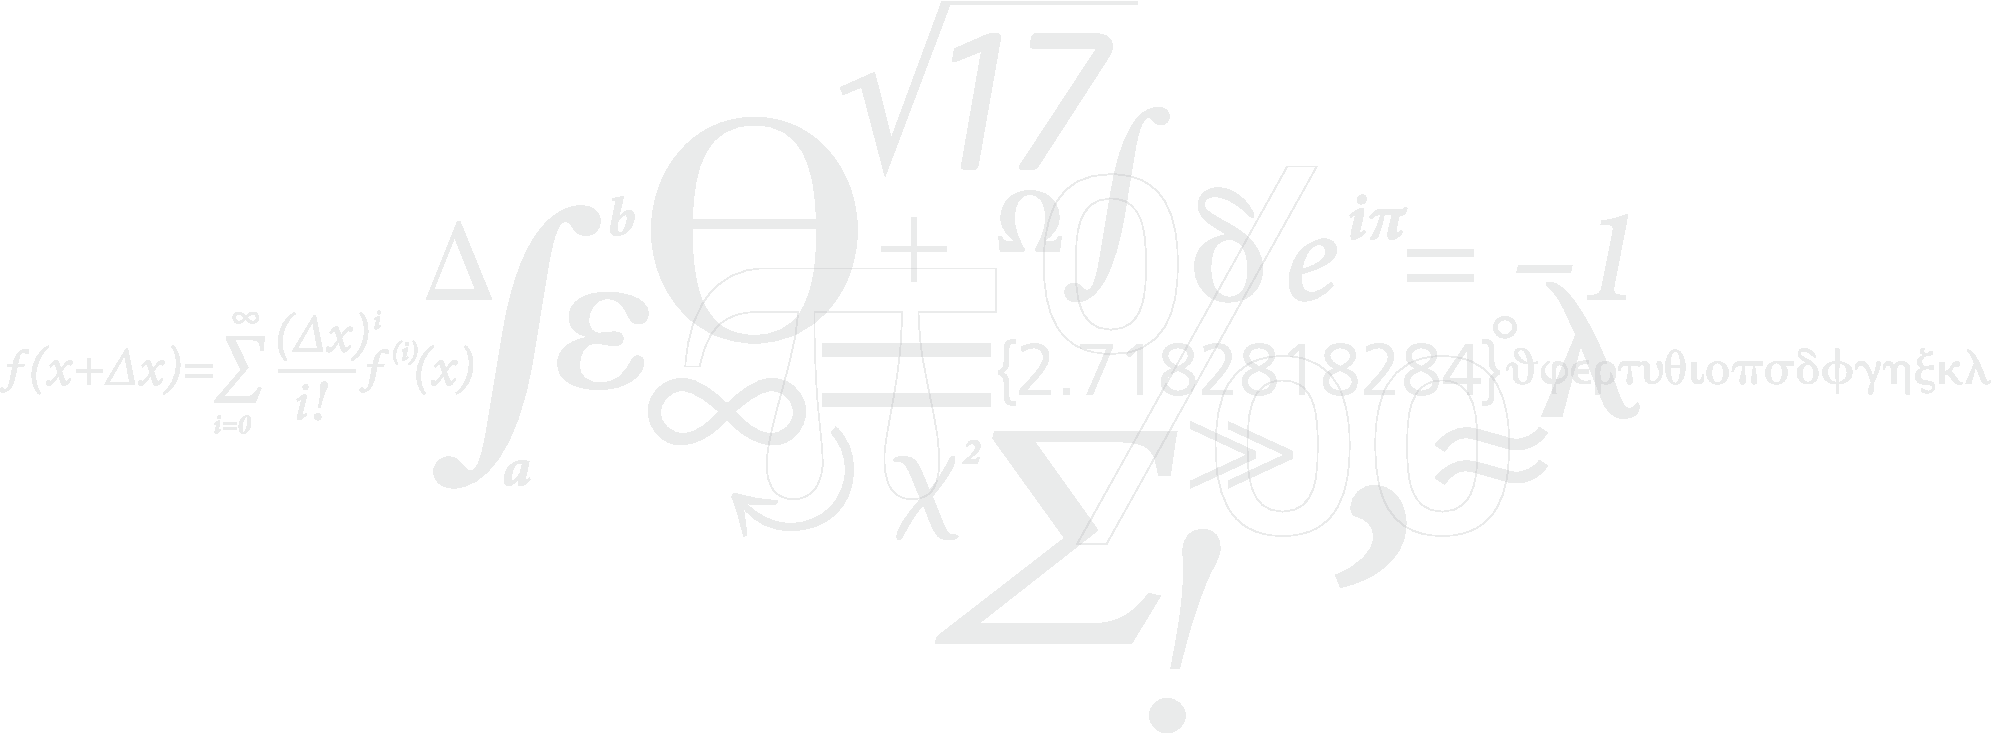
\includegraphics[trim=130mm 0 0 0,width=0.9\textwidth]{DTU-frise-SH-15}
                \vspace*{2.5cm}
            }
        }
    }
}

% This is a double sided book. If there is a last empty page lets use it for some fun e.g. the frieze.
% NB: For a fully functional hack the \clearpage used in \include does some odd thinks with the sequence numbering. Thefore use \input instead of \include at the end of the book. If bibliography is used at last everything should be ok.
\makeatletter
% Adjust so gatherings is allowed for single sheets too! (hacking functions in memoir.dtx)
\patchcmd{\leavespergathering}{\ifnum\@memcnta<\tw@}{\ifnum\@memcnta<\@ne}{
    \leavespergathering{1}
    % Insert the frieze
    \patchcmd{\@memensuresigpages}{\repeat}{\repeat\frieze}{}{}
}{}
\makeatother

%!TEX root = ../Thesis.tex

% Text fonts (http://www.macfreek.nl/memory/Fonts_in_LaTeX)
% Install fonts from /usr/local/texlive/<version>/texmf-dist/fonts/opentype/public
\usepackage{fontspec}

% Sans-serif font
\setsansfont[
    Ligatures=TeX,
    Extension=.otf,
    UprightFont=*-regular,
    BoldFont=*-bold,
    ItalicFont=*-italic,
    BoldItalicFont=*-bolditalic,
    %SlantedFont=,
    %BoldSlantedFont=,
    %SmallCapsFont=
]{texgyreadventor}

%\setsansfont[Ligatures=TeX]{Neo Sans Intel}    % Neo Sans Intel – Like DTU font but more symbols
%\setsansfont[Ligatures=TeX]{NeoSans}           % NeoSans – DTU font (missing `+' symbols and other)
%\setsansfont[Ligatures=TeX]{CMU Sans Serif}    % Computer Modern Unicode font
%\setsansfont[Ligatures=TeX]{Latin Modern Sans} % Latin Modern Sans serif font
%!TEX root = ../Thesis.tex

% Content specific packages.

\usepackage{blindtext}
\usepackage{algorithm}
\usepackage{algpseudocode}
\newcommand{\algorithmautorefname}{Algorithm}
\algnewcommand\algorithmicinitialize{\textbf{Initialize:}}
\algnewcommand\Initialize{\item[\algorithmicinitialize]}
\algnewcommand\algorithmicinput{\textbf{Input:}}
\algnewcommand\Input{\item[\algorithmicinput]}
\algnewcommand\algorithmicoutput{\textbf{Output:}}
\algnewcommand\Output{\item[\algorithmicoutput]}
% \usepackage{tikz}
% \usetikzlibrary{positioning, fit, arrows.meta, shapes}
\usepackage{pgfplots}                 % Plot tools
\usetikzlibrary{
    arrows.meta,
    matrix,
    positioning,
    shapes,
    topaths,
}
\pgfplotsset{compat=1.7}

% Listings
\lstset{
    aboveskip=0.8\baselineskip,
    basicstyle=\footnotesize\ttfamily,% the size of the fonts that are used for the code
    belowskip=-1.2\baselineskip,      % reset the belowskip to more reasonable value (baselineskip is redefined somewhere)
    breakatwhitespace=false,          % sets if automatic breaks should only happen at whitespace
    breaklines=true,                  % sets automatic line breaking
    captionpos=b,                     % sets the caption-position to bottom
    commentstyle=\color{s14a},        % comment style
    deletekeywords={sum},             % if you want to delete keywords from the given language
    escapeinside={\%*}{*)},           % if you want to add LaTeX within your code
    frame=single,                     % adds a frame around the code
    keywordstyle=\bfseries\ttfamily\color{s09}, % keyword style
    language=Python,                  % the language of the code
    morekeywords={*,...},             % if you want to add more keywords to the set
    numbers=left,                     % where to put the line-numbers; possible values are (none, left, right)
    numbersep=5pt,                    % how far the line-numbers are from the code
    numberstyle=\sffamily\tiny\color{dtugray}, % the style that is used for the line-numbers
    rulecolor=\color{dtugray},        % if not set, the frame-color may be changed on line-breaks within not-black text (e.g. %comments (green here))
    showspaces=false,                 % show spaces everywhere adding particular underscores; it overrides 'showstringspaces'
    showstringspaces=false,           % underline spaces within strings only
    showtabs=false,                   % show tabs within strings adding particular underscores
    stepnumber=1,                     % the step between two line-numbers. If it's 1, each line will be numbered
    stringstyle=\color{s07},          % string literal style
    tabsize=2,                        % sets default tabsize to 2 spaces
    title=\lstname,                   % show the filename of files included with \lstinputlisting; also try caption instead of title
}


%!TEX root = ../Thesis.tex

% Parenthesis
\providecommand{\pa}[1]{{\left(#1\right)}}
\renewcommand{\pa}[1]{{\left(#1\right)}}
\providecommand{\bra}[1]{{\left[#1\right]}}
\renewcommand{\bra}[1]{{\left[#1\right]}}
\providecommand{\cbra}[1]{{\left\{#1\right\}}}
\renewcommand{\cbra}[1]{{\left\{#1\right\}}}
\providecommand{\vbra}[1]{{\left\langle#1\right\rangle}}
\renewcommand{\vbra}[1]{{\left\langle#1\right\rangle}}

% Matrices for displayed expressions
\providecommand{\mat}[1]{{\begin{matrix}#1\end{matrix}}}
\renewcommand{\mat}[1]{{\begin{matrix}#1\end{matrix}}}
\providecommand{\pmat}[1]{{\begin{pmatrix}#1\end{pmatrix}}}
\renewcommand{\pmat}[1]{{\begin{pmatrix}#1\end{pmatrix}}}
\providecommand{\bmat}[1]{{\begin{bmatrix}#1\end{bmatrix}}}
\renewcommand{\bmat}[1]{{\begin{bmatrix}#1\end{bmatrix}}}

% Variations of \frac and \sfrac
\providecommand{\pfrac}[2]{{\left(\frac{#1}{#2}\right)}}
\renewcommand{\pfrac}[2]{{\left(\frac{#1}{#2}\right)}}
\providecommand{\bfrac}[2]{{\left[\frac{#1}{#2}\right]}}
\renewcommand{\bfrac}[2]{{\left[\frac{#1}{#2}\right]}}
\providecommand{\psfrac}[2]{{\left(\sfrac{#1}{#2}\right)}}
\renewcommand{\psfrac}[2]{{\left(\sfrac{#1}{#2}\right)}}
\providecommand{\bsfrac}[2]{{\left[\sfrac{#1}{#2}\right]}}
\renewcommand{\bsfrac}[2]{{\left[\sfrac{#1}{#2}\right]}}

% for small matrices to be used in in-line expressions
\providecommand{\sm}[1]{{\left\{#1\right\}}}
\renewcommand{\sm}[1]{{\left\{#1\right\}}}
\providecommand{\psm}[1]{{\pa{\sm{#1}}}}
\renewcommand{\psm}[1]{{\pa{\sm{#1}}}}
\providecommand{\bsm}[1]{{\bra{\sm{#1}}}}
\renewcommand{\bsm}[1]{{\bra{\sm{#1}}}}

% Norm
\providecommand{\norm}[1]{{\left\lVert#1\right\rVert}}
\renewcommand{\norm}[1]{{\left\lVert#1\right\rVert}}
% Size
\providecommand{\size}[1]{{\left\lvert#1\right\rvert}}
\renewcommand{\size}[1]{{\left\lvert#1\right\rvert}}
% Trace
\providecommand{\Tr}[1]{{\text{Tr}\left[#1\right]}}
\renewcommand{\Tr}[1]{{\text{Tr}\left[#1\right]}}
% Tranpose
\providecommand{\transpose}{{^\mathrm{T}}}
\renewcommand{\transpose}{{^\mathrm{T}}}

% Derivatives
\providecommand{\od}[3]{{\frac{\text{d}^{#3}#1}{\text{d}^{#3}#2}}}
\renewcommand{\od}[3]{{\frac{\text{d}^{#3}#1}{\text{d}^{#3}#2}}}
\providecommand{\pd}[3]{{\frac{\partial^{#3}#1}{\partial^{#3}#2}}}
\renewcommand{\pd}[3]{{\frac{\partial^{#3}#1}{\partial^{#3}#2}}}

% Bold upright letters
\providecommand{\a}{{\mathbf{a}}}
\renewcommand{\a}{{\mathbf{a}}}
\providecommand{\b}{{\mathbf{b}}}
\renewcommand{\b}{{\mathbf{b}}}
\providecommand{\c}{{\mathbf{c}}}
\renewcommand{\c}{{\mathbf{c}}}
\providecommand{\d}{{\mathbf{d}}}
\renewcommand{\d}{{\mathbf{d}}}
\providecommand{\e}{{\mathbf{e}}}
\renewcommand{\e}{{\mathbf{e}}}
\providecommand{\f}{{\mathbf{f}}}
\renewcommand{\f}{{\mathbf{f}}}
\providecommand{\g}{{\mathbf{g}}}
\renewcommand{\g}{{\mathbf{g}}}
\providecommand{\h}{{\mathbf{h}}}
\renewcommand{\h}{{\mathbf{h}}}
\providecommand{\i}{{\mathbf{i}}}
\renewcommand{\i}{{\mathbf{i}}}
\providecommand{\j}{{\mathbf{j}}}
\renewcommand{\j}{{\mathbf{j}}}
\providecommand{\k}{{\mathbf{k}}}
\renewcommand{\k}{{\mathbf{k}}}
\providecommand{\l}{{\mathbf{l}}}
\renewcommand{\l}{{\mathbf{l}}}
\providecommand{\m}{{\mathbf{m}}}
\renewcommand{\m}{{\mathbf{m}}}
\providecommand{\n}{{\mathbf{n}}}
\renewcommand{\n}{{\mathbf{n}}}
\providecommand{\o}{{\mathbf{o}}}
\renewcommand{\o}{{\mathbf{o}}}
\providecommand{\p}{{\mathbf{p}}}
\renewcommand{\p}{{\mathbf{p}}}
\providecommand{\q}{{\mathbf{q}}}
\renewcommand{\q}{{\mathbf{q}}}
\providecommand{\r}{{\mathbf{r}}}
\renewcommand{\r}{{\mathbf{r}}}
\providecommand{\s}{{\mathbf{s}}}
\renewcommand{\s}{{\mathbf{s}}}
\providecommand{\t}{{\mathbf{t}}}
\renewcommand{\t}{{\mathbf{t}}}
\providecommand{\u}{{\mathbf{u}}}
\renewcommand{\u}{{\mathbf{u}}}
\providecommand{\v}{{\mathbf{v}}}
\renewcommand{\v}{{\mathbf{v}}}
\providecommand{\w}{{\mathbf{w}}}
\renewcommand{\w}{{\mathbf{w}}}
\providecommand{\x}{{\mathbf{x}}}
\renewcommand{\x}{{\mathbf{x}}}
\providecommand{\y}{{\mathbf{y}}}
\renewcommand{\y}{{\mathbf{y}}}
\providecommand{\z}{{\mathbf{z}}}
\renewcommand{\z}{{\mathbf{z}}}
\providecommand{\A}{{\mathbf{A}}}
\renewcommand{\A}{{\mathbf{A}}}
\providecommand{\B}{{\mathbf{B}}}
\renewcommand{\B}{{\mathbf{B}}}
\providecommand{\C}{{\mathbf{C}}}
\renewcommand{\C}{{\mathbf{C}}}
\providecommand{\D}{{\mathbf{D}}}
\renewcommand{\D}{{\mathbf{D}}}
\providecommand{\E}{{\mathbf{E}}}
\renewcommand{\E}{{\mathbf{E}}}
\providecommand{\F}{{\mathbf{F}}}
\renewcommand{\F}{{\mathbf{F}}}
\providecommand{\G}{{\mathbf{G}}}
\renewcommand{\G}{{\mathbf{G}}}
\providecommand{\H}{{\mathbf{H}}}
\renewcommand{\H}{{\mathbf{H}}}
\providecommand{\I}{{\mathbf{I}}}
\renewcommand{\I}{{\mathbf{I}}}
\providecommand{\J}{{\mathbf{J}}}
\renewcommand{\J}{{\mathbf{J}}}
\providecommand{\K}{{\mathbf{K}}}
\renewcommand{\K}{{\mathbf{K}}}
\providecommand{\L}{{\mathbf{L}}}
\renewcommand{\L}{{\mathbf{L}}}
\providecommand{\M}{{\mathbf{M}}}
\renewcommand{\M}{{\mathbf{M}}}
\providecommand{\N}{{\mathbf{N}}}
\renewcommand{\N}{{\mathbf{N}}}
\providecommand{\O}{{\mathbf{O}}}
\renewcommand{\O}{{\mathbf{O}}}
\providecommand{\P}{{\mathbf{P}}}
\renewcommand{\P}{{\mathbf{P}}}
\providecommand{\Q}{{\mathbf{Q}}}
\renewcommand{\Q}{{\mathbf{Q}}}
\providecommand{\R}{{\mathbf{R}}}
\renewcommand{\R}{{\mathbf{R}}}
\providecommand{\S}{{\mathbf{S}}}
\renewcommand{\S}{{\mathbf{S}}}
\providecommand{\T}{{\mathbf{T}}}
\renewcommand{\T}{{\mathbf{T}}}
\providecommand{\U}{{\mathbf{U}}}
\renewcommand{\U}{{\mathbf{U}}}
\providecommand{\V}{{\mathbf{V}}}
\renewcommand{\V}{{\mathbf{V}}}
\providecommand{\W}{{\mathbf{W}}}
\renewcommand{\W}{{\mathbf{W}}}
\providecommand{\X}{{\mathbf{X}}}
\renewcommand{\X}{{\mathbf{X}}}
\providecommand{\Y}{{\mathbf{Y}}}
\renewcommand{\Y}{{\mathbf{Y}}}
\providecommand{\Z}{{\mathbf{Z}}}
\renewcommand{\Z}{{\mathbf{Z}}}
% Bold upright numbers
\providecommand{\0}{{\mathbf{0}}}
\renewcommand{\0}{{\mathbf{0}}}
\providecommand{\1}{{\mathbf{1}}}
\renewcommand{\1}{{\mathbf{1}}}
\providecommand{\2}{{\mathbf{2}}}
\renewcommand{\2}{{\mathbf{2}}}
\providecommand{\3}{{\mathbf{3}}}
\renewcommand{\3}{{\mathbf{3}}}
\providecommand{\4}{{\mathbf{4}}}
\renewcommand{\4}{{\mathbf{4}}}
\providecommand{\5}{{\mathbf{5}}}
\renewcommand{\5}{{\mathbf{5}}}
\providecommand{\6}{{\mathbf{6}}}
\renewcommand{\6}{{\mathbf{6}}}
\providecommand{\7}{{\mathbf{7}}}
\renewcommand{\7}{{\mathbf{7}}}
\providecommand{\8}{{\mathbf{8}}}
\renewcommand{\8}{{\mathbf{8}}}
\providecommand{\9}{{\mathbf{9}}}
\renewcommand{\9}{{\mathbf{9}}}
% Bold upright greek symbols
\providecommand{\alphab}{{\boldsymbol{\upalpha}}}
\renewcommand{\alphab}{{\boldsymbol{\upalpha}}}
\providecommand{\thetab}{{\boldsymbol{\uptheta}}}
\renewcommand{\thetab}{{\boldsymbol{\uptheta}}}
\providecommand{\taub}{{\boldsymbol{\uptau}}}
\renewcommand{\taub}{{\boldsymbol{\uptau}}}
\providecommand{\betab}{{\boldsymbol{\upbeta}}}
\renewcommand{\betab}{{\boldsymbol{\upbeta}}}
\providecommand{\varthetab}{{\boldsymbol{\upvartheta}}}
\renewcommand{\varthetab}{{\boldsymbol{\upvartheta}}}
\providecommand{\pib}{{\boldsymbol{\uppi}}}
\renewcommand{\pib}{{\boldsymbol{\uppi}}}
\providecommand{\upsilonb}{{\boldsymbol{\upupsilon}}}
\renewcommand{\upsilonb}{{\boldsymbol{\upupsilon}}}
\providecommand{\gammab}{{\boldsymbol{\upgamma}}}
\renewcommand{\gammab}{{\boldsymbol{\upgamma}}}
\providecommand{\gammab}{{\boldsymbol{\upgamma}}}
\renewcommand{\gammab}{{\boldsymbol{\upgamma}}}
\providecommand{\varpib}{{\boldsymbol{\upvarpi}}}
\renewcommand{\varpib}{{\boldsymbol{\upvarpi}}}
\providecommand{\phib}{{\boldsymbol{\upphi}}}
\renewcommand{\phib}{{\boldsymbol{\upphi}}}
\providecommand{\deltab}{{\boldsymbol{\updelta}}}
\renewcommand{\deltab}{{\boldsymbol{\updelta}}}
\providecommand{\kappab}{{\boldsymbol{\upkappa}}}
\renewcommand{\kappab}{{\boldsymbol{\upkappa}}}
\providecommand{\rhob}{{\boldsymbol{\uprho}}}
\renewcommand{\rhob}{{\boldsymbol{\uprho}}}
\providecommand{\varphib}{{\boldsymbol{\upvarphi}}}
\renewcommand{\varphib}{{\boldsymbol{\upvarphi}}}
\providecommand{\epsilonb}{{\boldsymbol{\upepsilon}}}
\renewcommand{\epsilonb}{{\boldsymbol{\upepsilon}}}
\providecommand{\lambdab}{{\boldsymbol{\uplambda}}}
\renewcommand{\lambdab}{{\boldsymbol{\uplambda}}}
\providecommand{\varrhob}{{\boldsymbol{\upvarrho}}}
\renewcommand{\varrhob}{{\boldsymbol{\upvarrho}}}
\providecommand{\chib}{{\boldsymbol{\upchi}}}
\renewcommand{\chib}{{\boldsymbol{\upchi}}}
\providecommand{\varepsilonb}{{\boldsymbol{\upvarepsilon}}}
\renewcommand{\varepsilonb}{{\boldsymbol{\upvarepsilon}}}
\providecommand{\mub}{{\boldsymbol{\upmu}}}
\renewcommand{\mub}{{\boldsymbol{\upmu}}}
\providecommand{\sigmab}{{\boldsymbol{\upsigma}}}
\renewcommand{\sigmab}{{\boldsymbol{\upsigma}}}
\providecommand{\psib}{{\boldsymbol{\uppsi}}}
\renewcommand{\psib}{{\boldsymbol{\uppsi}}}
\providecommand{\zetab}{{\boldsymbol{\upzeta}}}
\renewcommand{\zetab}{{\boldsymbol{\upzeta}}}
\providecommand{\nub}{{\boldsymbol{\upnu}}}
\renewcommand{\nub}{{\boldsymbol{\upnu}}}
\providecommand{\varsigmab}{{\boldsymbol{\upvarsigma}}}
\renewcommand{\varsigmab}{{\boldsymbol{\upvarsigma}}}
\providecommand{\omegab}{{\boldsymbol{\upomega}}}
\renewcommand{\omegab}{{\boldsymbol{\upomega}}}
\providecommand{\etab}{{\boldsymbol{\upeta}}}
\renewcommand{\etab}{{\boldsymbol{\upeta}}}
\providecommand{\xib}{{\boldsymbol{\upxi}}}
\renewcommand{\xib}{{\boldsymbol{\upxi}}}
\providecommand{\Gammab}{{\boldsymbol{\Upgamma}}}
\renewcommand{\Gammab}{{\boldsymbol{\Upgamma}}}
\providecommand{\Lambdab}{{\boldsymbol{\Uplambda}}}
\renewcommand{\Lambdab}{{\boldsymbol{\Uplambda}}}
\providecommand{\Sigmab}{{\boldsymbol{\Upsigma}}}
\renewcommand{\Sigmab}{{\boldsymbol{\Upsigma}}}
\providecommand{\Psib}{{\boldsymbol{\Uppsi}}}
\renewcommand{\Psib}{{\boldsymbol{\Uppsi}}}
\providecommand{\Deltab}{{\boldsymbol{\Updelta}}}
\renewcommand{\Deltab}{{\boldsymbol{\Updelta}}}
\providecommand{\Xib}{{\boldsymbol{\Upxi}}}
\renewcommand{\Xib}{{\boldsymbol{\Upxi}}}
\providecommand{\Upsilonb}{{\boldsymbol{\Upupsilon}}}
\renewcommand{\Upsilonb}{{\boldsymbol{\Upupsilon}}}
\providecommand{\Omegab}{{\boldsymbol{\Upomega}}}
\renewcommand{\Omegab}{{\boldsymbol{\Upomega}}}
\providecommand{\Thetab}{{\boldsymbol{\Uptheta}}}
\renewcommand{\Thetab}{{\boldsymbol{\Uptheta}}}
\providecommand{\Pib}{{\boldsymbol{\Uppi}}}
\renewcommand{\Pib}{{\boldsymbol{\Uppi}}}
\providecommand{\Phib}{{\boldsymbol{\Upphi}}}
\renewcommand{\Phib}{{\boldsymbol{\Upphi}}}

% Bold letters
\providecommand{\abs}{{{\boldsymbol{a}}}}
\renewcommand{\abs}{{{\boldsymbol{a}}}}
\providecommand{\bbs}{{{\boldsymbol{b}}}}
\renewcommand{\bbs}{{{\boldsymbol{b}}}}
\providecommand{\cbs}{{{\boldsymbol{c}}}}
\renewcommand{\cbs}{{{\boldsymbol{c}}}}
\providecommand{\dbs}{{{\boldsymbol{d}}}}
\renewcommand{\dbs}{{{\boldsymbol{d}}}}
\providecommand{\ebs}{{{\boldsymbol{e}}}}
\renewcommand{\ebs}{{{\boldsymbol{e}}}}
\providecommand{\fbs}{{{\boldsymbol{f}}}}
\renewcommand{\fbs}{{{\boldsymbol{f}}}}
\providecommand{\gbs}{{{\boldsymbol{g}}}}
\renewcommand{\gbs}{{{\boldsymbol{g}}}}
\providecommand{\hbs}{{{\boldsymbol{h}}}}
\renewcommand{\hbs}{{{\boldsymbol{h}}}}
\providecommand{\ibs}{{{\boldsymbol{i}}}}
\renewcommand{\ibs}{{{\boldsymbol{i}}}}
\providecommand{\jbs}{{{\boldsymbol{j}}}}
\renewcommand{\jbs}{{{\boldsymbol{j}}}}
\providecommand{\kbs}{{{\boldsymbol{k}}}}
\renewcommand{\kbs}{{{\boldsymbol{k}}}}
\providecommand{\lbs}{{{\boldsymbol{l}}}}
\renewcommand{\lbs}{{{\boldsymbol{l}}}}
\providecommand{\mbs}{{{\boldsymbol{m}}}}
\renewcommand{\mbs}{{{\boldsymbol{m}}}}
\providecommand{\nbs}{{{\boldsymbol{n}}}}
\renewcommand{\nbs}{{{\boldsymbol{n}}}}
\providecommand{\obs}{{{\boldsymbol{o}}}}
\renewcommand{\obs}{{{\boldsymbol{o}}}}
\providecommand{\pbs}{{{\boldsymbol{p}}}}
\renewcommand{\pbs}{{{\boldsymbol{p}}}}
\providecommand{\qbs}{{{\boldsymbol{q}}}}
\renewcommand{\qbs}{{{\boldsymbol{q}}}}
\providecommand{\rbs}{{{\boldsymbol{r}}}}
\renewcommand{\rbs}{{{\boldsymbol{r}}}}
\providecommand{\sbs}{{{\boldsymbol{s}}}}
\renewcommand{\sbs}{{{\boldsymbol{s}}}}
\providecommand{\tbs}{{{\boldsymbol{t}}}}
\renewcommand{\tbs}{{{\boldsymbol{t}}}}
\providecommand{\ubs}{{{\boldsymbol{u}}}}
\renewcommand{\ubs}{{{\boldsymbol{u}}}}
\providecommand{\vbs}{{{\boldsymbol{v}}}}
\renewcommand{\vbs}{{{\boldsymbol{v}}}}
\providecommand{\wbs}{{{\boldsymbol{w}}}}
\renewcommand{\wbs}{{{\boldsymbol{w}}}}
\providecommand{\xbs}{{{\boldsymbol{x}}}}
\renewcommand{\xbs}{{{\boldsymbol{x}}}}
\providecommand{\ybs}{{{\boldsymbol{y}}}}
\renewcommand{\ybs}{{{\boldsymbol{y}}}}
\providecommand{\zbs}{{{\boldsymbol{z}}}}
\renewcommand{\zbs}{{{\boldsymbol{z}}}}
\providecommand{\Abs}{{{\boldsymbol{A}}}}
\renewcommand{\Abs}{{{\boldsymbol{A}}}}
\providecommand{\Bbs}{{{\boldsymbol{B}}}}
\renewcommand{\Bbs}{{{\boldsymbol{B}}}}
\providecommand{\Cbs}{{{\boldsymbol{C}}}}
\renewcommand{\Cbs}{{{\boldsymbol{C}}}}
\providecommand{\Dbs}{{{\boldsymbol{D}}}}
\renewcommand{\Dbs}{{{\boldsymbol{D}}}}
\providecommand{\Ebs}{{{\boldsymbol{E}}}}
\renewcommand{\Ebs}{{{\boldsymbol{E}}}}
\providecommand{\Fbs}{{{\boldsymbol{F}}}}
\renewcommand{\Fbs}{{{\boldsymbol{F}}}}
\providecommand{\Gbs}{{{\boldsymbol{G}}}}
\renewcommand{\Gbs}{{{\boldsymbol{G}}}}
\providecommand{\Hbs}{{{\boldsymbol{H}}}}
\renewcommand{\Hbs}{{{\boldsymbol{H}}}}
\providecommand{\Ibs}{{{\boldsymbol{I}}}}
\renewcommand{\Ibs}{{{\boldsymbol{I}}}}
\providecommand{\Jbs}{{{\boldsymbol{J}}}}
\renewcommand{\Jbs}{{{\boldsymbol{J}}}}
\providecommand{\Kbs}{{{\boldsymbol{K}}}}
\renewcommand{\Kbs}{{{\boldsymbol{K}}}}
\providecommand{\Lbs}{{{\boldsymbol{L}}}}
\renewcommand{\Lbs}{{{\boldsymbol{L}}}}
\providecommand{\Mbs}{{{\boldsymbol{M}}}}
\renewcommand{\Mbs}{{{\boldsymbol{M}}}}
\providecommand{\Nbs}{{{\boldsymbol{N}}}}
\renewcommand{\Nbs}{{{\boldsymbol{N}}}}
\providecommand{\Obs}{{{\boldsymbol{O}}}}
\renewcommand{\Obs}{{{\boldsymbol{O}}}}
\providecommand{\Pbs}{{{\boldsymbol{P}}}}
\renewcommand{\Pbs}{{{\boldsymbol{P}}}}
\providecommand{\Qbs}{{{\boldsymbol{Q}}}}
\renewcommand{\Qbs}{{{\boldsymbol{Q}}}}
\providecommand{\Rbs}{{{\boldsymbol{R}}}}
\renewcommand{\Rbs}{{{\boldsymbol{R}}}}
\providecommand{\Sbs}{{{\boldsymbol{S}}}}
\renewcommand{\Sbs}{{{\boldsymbol{S}}}}
\providecommand{\Tbs}{{{\boldsymbol{T}}}}
\renewcommand{\Tbs}{{{\boldsymbol{T}}}}
\providecommand{\Ubs}{{{\boldsymbol{U}}}}
\renewcommand{\Ubs}{{{\boldsymbol{U}}}}
\providecommand{\Vbs}{{{\boldsymbol{V}}}}
\renewcommand{\Vbs}{{{\boldsymbol{V}}}}
\providecommand{\Wbs}{{{\boldsymbol{W}}}}
\renewcommand{\Wbs}{{{\boldsymbol{W}}}}
\providecommand{\Xbs}{{{\boldsymbol{X}}}}
\renewcommand{\Xbs}{{{\boldsymbol{X}}}}
\providecommand{\Ybs}{{{\boldsymbol{Y}}}}
\renewcommand{\Ybs}{{{\boldsymbol{Y}}}}
\providecommand{\Zbs}{{{\boldsymbol{Z}}}}
\renewcommand{\Zbs}{{{\boldsymbol{Z}}}}
% Bold greek symbols
\providecommand{\alphabs}{{{\boldsymbol{\alpha}}}}
\renewcommand{\alphabs}{{{\boldsymbol{\alpha}}}}
\providecommand{\thetabs}{{{\boldsymbol{\theta}}}}
\renewcommand{\thetabs}{{{\boldsymbol{\theta}}}}
\providecommand{\taubs}{{{\boldsymbol{\tau}}}}
\renewcommand{\taubs}{{{\boldsymbol{\tau}}}}
\providecommand{\betabs}{{{\boldsymbol{\beta}}}}
\renewcommand{\betabs}{{{\boldsymbol{\beta}}}}
\providecommand{\varthetabs}{{{\boldsymbol{\vartheta}}}}
\renewcommand{\varthetabs}{{{\boldsymbol{\vartheta}}}}
\providecommand{\pibs}{{{\boldsymbol{\pi}}}}
\renewcommand{\pibs}{{{\boldsymbol{\pi}}}}
\providecommand{\upsilonbs}{{{\boldsymbol{\upsilon}}}}
\renewcommand{\upsilonbs}{{{\boldsymbol{\upsilon}}}}
\providecommand{\gammabs}{{{\boldsymbol{\gamma}}}}
\renewcommand{\gammabs}{{{\boldsymbol{\gamma}}}}
\providecommand{\gammabs}{{{\boldsymbol{\gamma}}}}
\renewcommand{\gammabs}{{{\boldsymbol{\gamma}}}}
\providecommand{\varpibs}{{{\boldsymbol{\varpi}}}}
\renewcommand{\varpibs}{{{\boldsymbol{\varpi}}}}
\providecommand{\phibs}{{{\boldsymbol{\phi}}}}
\renewcommand{\phibs}{{{\boldsymbol{\phi}}}}
\providecommand{\deltabs}{{{\boldsymbol{\delta}}}}
\renewcommand{\deltabs}{{{\boldsymbol{\delta}}}}
\providecommand{\kappabs}{{{\boldsymbol{\kappa}}}}
\renewcommand{\kappabs}{{{\boldsymbol{\kappa}}}}
\providecommand{\rhobs}{{{\boldsymbol{\rho}}}}
\renewcommand{\rhobs}{{{\boldsymbol{\rho}}}}
\providecommand{\varphibs}{{{\boldsymbol{\varphi}}}}
\renewcommand{\varphibs}{{{\boldsymbol{\varphi}}}}
\providecommand{\epsilonbs}{{{\boldsymbol{\epsilon}}}}
\renewcommand{\epsilonbs}{{{\boldsymbol{\epsilon}}}}
\providecommand{\lambdabs}{{{\boldsymbol{\lambda}}}}
\renewcommand{\lambdabs}{{{\boldsymbol{\lambda}}}}
\providecommand{\varrhobs}{{{\boldsymbol{\varrho}}}}
\renewcommand{\varrhobs}{{{\boldsymbol{\varrho}}}}
\providecommand{\chibs}{{{\boldsymbol{\chi}}}}
\renewcommand{\chibs}{{{\boldsymbol{\chi}}}}
\providecommand{\varepsilonbs}{{{\boldsymbol{\varepsilon}}}}
\renewcommand{\varepsilonbs}{{{\boldsymbol{\varepsilon}}}}
\providecommand{\mubs}{{{\boldsymbol{\mu}}}}
\renewcommand{\mubs}{{{\boldsymbol{\mu}}}}
\providecommand{\sigmabs}{{{\boldsymbol{\sigma}}}}
\renewcommand{\sigmabs}{{{\boldsymbol{\sigma}}}}
\providecommand{\psibs}{{{\boldsymbol{\psi}}}}
\renewcommand{\psibs}{{{\boldsymbol{\psi}}}}
\providecommand{\zetabs}{{{\boldsymbol{\zeta}}}}
\renewcommand{\zetabs}{{{\boldsymbol{\zeta}}}}
\providecommand{\nubs}{{{\boldsymbol{\nu}}}}
\renewcommand{\nubs}{{{\boldsymbol{\nu}}}}
\providecommand{\varsigmabs}{{{\boldsymbol{\varsigma}}}}
\renewcommand{\varsigmabs}{{{\boldsymbol{\varsigma}}}}
\providecommand{\omegabs}{{{\boldsymbol{\omega}}}}
\renewcommand{\omegabs}{{{\boldsymbol{\omega}}}}
\providecommand{\etabs}{{{\boldsymbol{\eta}}}}
\renewcommand{\etabs}{{{\boldsymbol{\eta}}}}
\providecommand{\xibs}{{{\boldsymbol{\xi}}}}
\renewcommand{\xibs}{{{\boldsymbol{\xi}}}}
\providecommand{\Gammabs}{{{\boldsymbol{\Gamma}}}}
\renewcommand{\Gammabs}{{{\boldsymbol{\Gamma}}}}
\providecommand{\Lambdabs}{{{\boldsymbol{\Lambda}}}}
\renewcommand{\Lambdabs}{{{\boldsymbol{\Lambda}}}}
\providecommand{\Sigmabs}{{{\boldsymbol{\Sigma}}}}
\renewcommand{\Sigmabs}{{{\boldsymbol{\Sigma}}}}
\providecommand{\Psibs}{{{\boldsymbol{\Psi}}}}
\renewcommand{\Psibs}{{{\boldsymbol{\Psi}}}}
\providecommand{\Deltabs}{{{\boldsymbol{\Delta}}}}
\renewcommand{\Deltabs}{{{\boldsymbol{\Delta}}}}
\providecommand{\Xibs}{{{\boldsymbol{\Xi}}}}
\renewcommand{\Xibs}{{{\boldsymbol{\Xi}}}}
\providecommand{\Upsilonbs}{{{\boldsymbol{\Upsilon}}}}
\renewcommand{\Upsilonbs}{{{\boldsymbol{\Upsilon}}}}
\providecommand{\Omegabs}{{{\boldsymbol{\Omega}}}}
\renewcommand{\Omegabs}{{{\boldsymbol{\Omega}}}}
\providecommand{\Thetabs}{{{\boldsymbol{\Theta}}}}
\renewcommand{\Thetabs}{{{\boldsymbol{\Theta}}}}
\providecommand{\Pibs}{{{\boldsymbol{\Pi}}}}
\renewcommand{\Pibs}{{{\boldsymbol{\Pi}}}}
\providecommand{\Phibs}{{{\boldsymbol{\Phi}}}}
\renewcommand{\Phibs}{{{\boldsymbol{\Phi}}}}

% \mathbb{} shortcuts
\providecommand{\abb}{{\mathbb{a}}}
\renewcommand{\abb}{{\mathbb{a}}}
\providecommand{\bbb}{{\mathbb{b}}}
\renewcommand{\bbb}{{\mathbb{b}}}
\providecommand{\cbb}{{\mathbb{c}}}
\renewcommand{\cbb}{{\mathbb{c}}}
\providecommand{\dbb}{{\mathbb{d}}}
\renewcommand{\dbb}{{\mathbb{d}}}
\providecommand{\ebb}{{\mathbb{e}}}
\renewcommand{\ebb}{{\mathbb{e}}}
\providecommand{\fbb}{{\mathbb{f}}}
\renewcommand{\fbb}{{\mathbb{f}}}
\providecommand{\gbb}{{\mathbb{g}}}
\renewcommand{\gbb}{{\mathbb{g}}}
\providecommand{\hbb}{{\mathbb{h}}}
\renewcommand{\hbb}{{\mathbb{h}}}
\providecommand{\ibb}{{\mathbb{i}}}
\renewcommand{\ibb}{{\mathbb{i}}}
\providecommand{\jbb}{{\mathbb{j}}}
\renewcommand{\jbb}{{\mathbb{j}}}
\providecommand{\kbb}{{\mathbb{k}}}
\renewcommand{\kbb}{{\mathbb{k}}}
\providecommand{\lbb}{{\mathbb{l}}}
\renewcommand{\lbb}{{\mathbb{l}}}
\providecommand{\mbb}{{\mathbb{m}}}
\renewcommand{\mbb}{{\mathbb{m}}}
\providecommand{\nbb}{{\mathbb{n}}}
\renewcommand{\nbb}{{\mathbb{n}}}
\providecommand{\obb}{{\mathbb{o}}}
\renewcommand{\obb}{{\mathbb{o}}}
\providecommand{\pbb}{{\mathbb{p}}}
\renewcommand{\pbb}{{\mathbb{p}}}
\providecommand{\qbb}{{\mathbb{q}}}
\renewcommand{\qbb}{{\mathbb{q}}}
\providecommand{\rbb}{{\mathbb{r}}}
\renewcommand{\rbb}{{\mathbb{r}}}
\providecommand{\sbb}{{\mathbb{s}}}
\renewcommand{\sbb}{{\mathbb{s}}}
\providecommand{\tbb}{{\mathbb{t}}}
\renewcommand{\tbb}{{\mathbb{t}}}
\providecommand{\ubb}{{\mathbb{u}}}
\renewcommand{\ubb}{{\mathbb{u}}}
\providecommand{\vbb}{{\mathbb{v}}}
\renewcommand{\vbb}{{\mathbb{v}}}
\providecommand{\wbb}{{\mathbb{w}}}
\renewcommand{\wbb}{{\mathbb{w}}}
\providecommand{\xbb}{{\mathbb{x}}}
\renewcommand{\xbb}{{\mathbb{x}}}
\providecommand{\ybb}{{\mathbb{y}}}
\renewcommand{\ybb}{{\mathbb{y}}}
\providecommand{\zbb}{{\mathbb{z}}}
\renewcommand{\zbb}{{\mathbb{z}}}
\providecommand{\Abb}{{\mathbb{A}}}
\renewcommand{\Abb}{{\mathbb{A}}}
\providecommand{\Bbb}{{\mathbb{B}}}
\renewcommand{\Bbb}{{\mathbb{B}}}
\providecommand{\Cbb}{{\mathbb{C}}}
\renewcommand{\Cbb}{{\mathbb{C}}}
\providecommand{\Dbb}{{\mathbb{D}}}
\renewcommand{\Dbb}{{\mathbb{D}}}
\providecommand{\Ebb}{{\mathbb{E}}}
\renewcommand{\Ebb}{{\mathbb{E}}}
\providecommand{\Fbb}{{\mathbb{F}}}
\renewcommand{\Fbb}{{\mathbb{F}}}
\providecommand{\Gbb}{{\mathbb{G}}}
\renewcommand{\Gbb}{{\mathbb{G}}}
\providecommand{\Hbb}{{\mathbb{H}}}
\renewcommand{\Hbb}{{\mathbb{H}}}
\providecommand{\Ibb}{{\mathbb{I}}}
\renewcommand{\Ibb}{{\mathbb{I}}}
\providecommand{\Jbb}{{\mathbb{J}}}
\renewcommand{\Jbb}{{\mathbb{J}}}
\providecommand{\Kbb}{{\mathbb{K}}}
\renewcommand{\Kbb}{{\mathbb{K}}}
\providecommand{\Lbb}{{\mathbb{L}}}
\renewcommand{\Lbb}{{\mathbb{L}}}
\providecommand{\Mbb}{{\mathbb{M}}}
\renewcommand{\Mbb}{{\mathbb{M}}}
\providecommand{\Nbb}{{\mathbb{N}}}
\renewcommand{\Nbb}{{\mathbb{N}}}
\providecommand{\Obb}{{\mathbb{O}}}
\renewcommand{\Obb}{{\mathbb{O}}}
\providecommand{\Pbb}{{\mathbb{P}}}
\renewcommand{\Pbb}{{\mathbb{P}}}
\providecommand{\Qbb}{{\mathbb{Q}}}
\renewcommand{\Qbb}{{\mathbb{Q}}}
\providecommand{\Rbb}{{\mathbb{R}}}
\renewcommand{\Rbb}{{\mathbb{R}}}
\providecommand{\Sbb}{{\mathbb{S}}}
\renewcommand{\Sbb}{{\mathbb{S}}}
\providecommand{\Tbb}{{\mathbb{T}}}
\renewcommand{\Tbb}{{\mathbb{T}}}
\providecommand{\Ubb}{{\mathbb{U}}}
\renewcommand{\Ubb}{{\mathbb{U}}}
\providecommand{\Vbb}{{\mathbb{V}}}
\renewcommand{\Vbb}{{\mathbb{V}}}
\providecommand{\Wbb}{{\mathbb{W}}}
\renewcommand{\Wbb}{{\mathbb{W}}}
\providecommand{\Xbb}{{\mathbb{X}}}
\renewcommand{\Xbb}{{\mathbb{X}}}
\providecommand{\Ybb}{{\mathbb{Y}}}
\renewcommand{\Ybb}{{\mathbb{Y}}}
\providecommand{\Zbb}{{\mathbb{Z}}}
\renewcommand{\Zbb}{{\mathbb{Z}}}

% \mathcal{} shortcuts
\providecommand{\ac}{{\mathcal{a}}}
\renewcommand{\ac}{{\mathcal{a}}}
\providecommand{\bc}{{\mathcal{b}}}
\renewcommand{\bc}{{\mathcal{b}}}
\providecommand{\cc}{{\mathcal{c}}}
\renewcommand{\cc}{{\mathcal{c}}}
\providecommand{\dc}{{\mathcal{d}}}
\renewcommand{\dc}{{\mathcal{d}}}
\providecommand{\ec}{{\mathcal{e}}}
\renewcommand{\ec}{{\mathcal{e}}}
\providecommand{\fc}{{\mathcal{f}}}
\renewcommand{\fc}{{\mathcal{f}}}
\providecommand{\gc}{{\mathcal{g}}}
\renewcommand{\gc}{{\mathcal{g}}}
\providecommand{\hc}{{\mathcal{h}}}
\renewcommand{\hc}{{\mathcal{h}}}
\providecommand{\ic}{{\mathcal{i}}}
\renewcommand{\ic}{{\mathcal{i}}}
\providecommand{\jc}{{\mathcal{j}}}
\renewcommand{\jc}{{\mathcal{j}}}
\providecommand{\kc}{{\mathcal{k}}}
\renewcommand{\kc}{{\mathcal{k}}}
\providecommand{\lc}{{\mathcal{l}}}
\renewcommand{\lc}{{\mathcal{l}}}
\providecommand{\mc}{{\mathcal{m}}}
\renewcommand{\mc}{{\mathcal{m}}}
\providecommand{\nc}{{\mathcal{n}}}
\renewcommand{\nc}{{\mathcal{n}}}
\providecommand{\oc}{{\mathcal{o}}}
\renewcommand{\oc}{{\mathcal{o}}}
\providecommand{\pc}{{\mathcal{p}}}
\renewcommand{\pc}{{\mathcal{p}}}
\providecommand{\qc}{{\mathcal{q}}}
\renewcommand{\qc}{{\mathcal{q}}}
\providecommand{\rc}{{\mathcal{r}}}
\renewcommand{\rc}{{\mathcal{r}}}
\providecommand{\sc}{{\mathcal{s}}}
\renewcommand{\sc}{{\mathcal{s}}}
\providecommand{\tc}{{\mathcal{t}}}
\renewcommand{\tc}{{\mathcal{t}}}
\providecommand{\uc}{{\mathcal{u}}}
\renewcommand{\uc}{{\mathcal{u}}}
\providecommand{\vc}{{\mathcal{v}}}
\renewcommand{\vc}{{\mathcal{v}}}
\providecommand{\wc}{{\mathcal{w}}}
\renewcommand{\wc}{{\mathcal{w}}}
\providecommand{\xc}{{\mathcal{x}}}
\renewcommand{\xc}{{\mathcal{x}}}
\providecommand{\yc}{{\mathcal{y}}}
\renewcommand{\yc}{{\mathcal{y}}}
\providecommand{\zc}{{\mathcal{z}}}
\renewcommand{\zc}{{\mathcal{z}}}
\providecommand{\Ac}{{\mathcal{A}}}
\renewcommand{\Ac}{{\mathcal{A}}}
\providecommand{\Bc}{{\mathcal{B}}}
\renewcommand{\Bc}{{\mathcal{B}}}
\providecommand{\Cc}{{\mathcal{C}}}
\renewcommand{\Cc}{{\mathcal{C}}}
\providecommand{\Dc}{{\mathcal{D}}}
\renewcommand{\Dc}{{\mathcal{D}}}
\providecommand{\Ec}{{\mathcal{E}}}
\renewcommand{\Ec}{{\mathcal{E}}}
\providecommand{\Fc}{{\mathcal{F}}}
\renewcommand{\Fc}{{\mathcal{F}}}
\providecommand{\Gc}{{\mathcal{G}}}
\renewcommand{\Gc}{{\mathcal{G}}}
\providecommand{\Hc}{{\mathcal{H}}}
\renewcommand{\Hc}{{\mathcal{H}}}
\providecommand{\Ic}{{\mathcal{I}}}
\renewcommand{\Ic}{{\mathcal{I}}}
\providecommand{\Jc}{{\mathcal{J}}}
\renewcommand{\Jc}{{\mathcal{J}}}
\providecommand{\Kc}{{\mathcal{K}}}
\renewcommand{\Kc}{{\mathcal{K}}}
\providecommand{\Lc}{{\mathcal{L}}}
\renewcommand{\Lc}{{\mathcal{L}}}
\providecommand{\Mc}{{\mathcal{M}}}
\renewcommand{\Mc}{{\mathcal{M}}}
\providecommand{\Nc}{{\mathcal{N}}}
\renewcommand{\Nc}{{\mathcal{N}}}
\providecommand{\Oc}{{\mathcal{O}}}
\renewcommand{\Oc}{{\mathcal{O}}}
\providecommand{\Pc}{{\mathcal{P}}}
\renewcommand{\Pc}{{\mathcal{P}}}
\providecommand{\Qc}{{\mathcal{Q}}}
\renewcommand{\Qc}{{\mathcal{Q}}}
\providecommand{\Rc}{{\mathcal{R}}}
\renewcommand{\Rc}{{\mathcal{R}}}
\providecommand{\Sc}{{\mathcal{S}}}
\renewcommand{\Sc}{{\mathcal{S}}}
\providecommand{\Tc}{{\mathcal{T}}}
\renewcommand{\Tc}{{\mathcal{T}}}
\providecommand{\Uc}{{\mathcal{U}}}
\renewcommand{\Uc}{{\mathcal{U}}}
\providecommand{\Vc}{{\mathcal{V}}}
\renewcommand{\Vc}{{\mathcal{V}}}
\providecommand{\Wc}{{\mathcal{W}}}
\renewcommand{\Wc}{{\mathcal{W}}}
\providecommand{\Xc}{{\mathcal{X}}}
\renewcommand{\Xc}{{\mathcal{X}}}
\providecommand{\Yc}{{\mathcal{Y}}}
\renewcommand{\Yc}{{\mathcal{Y}}}
\providecommand{\Zc}{{\mathcal{Z}}}
\renewcommand{\Zc}{{\mathcal{Z}}}


%!TEX root = ../Thesis.tex

%\makeglossaries
\makenoidxglossaries

% Abbreviations
\newacronym{AI}{AI}{artificial intelligence}
\newacronym{ML}{ML}{machine learning}
\newacronym{DL}{DL}{deep learning}
\newacronym{RL}{RL}{reinforcement learning}
\newacronym{DRL}{DRL}{deep reinforcement learning}

\newacronym{MDP}{MDP}{Markov decision process}

\newacronym{NN}{NN}{neural network}
\newacronym{MLP}{MLP}{multilayer perceptron}
\newacronym{FNN}{FNN}{feedforward neural network}
\newacronym{CNN}{CNN}{convolutional neural network}
\newacronym{RNN}{RNN}{recurrent neural network}
\newacronym{LSTM}{LSTM}{long short-term memory}
\newacronym{GRU}{GRU}{gated recurrent unit}
\newacronym{BNN}{BNN}{Bayesian neural network}

\newacronym{ReLU}{ReLU}{rectified linear unit}

\newacronym{SGD}{SGD}{stochastic gradient descent}
\newacronym[longplural={evolution strategies}]{ES}{ES}{evolution stategy}
\newacronym{VO}{VO}{variational optimization}
\newacronym{SGVB}{SGVB}{stochastic gradient variational Bayes}

\newacronym{NLL}{NLL}{negative log-likelihood}
\newacronym{MSE}{MSE}{mean squared error}
\newacronym{CEL}{CEL}{cross entropy loss}
\newacronym{MLE}{MLE}{maximum likelihood estimate}

\newacronym{SVD}{SVD}{singular value decomposition}

\newacronym{SMG}{SM-G}{safe mutations through gradients}

\newacronym{PCA}{PCA}{principal components analysis}
\newacronym{GP}{GP}{Gaussian process}
\newacronym{CMA-ES}{CMA-ES}{Covariance Matrix Adaptation Evolution Strategy}

\newacronym{PDF}{PDF}{probability density function}
\newacronym[longplural={Fisher information matrices}]{FIM}{FIM}{Fisher information matrix}
\newacronym{KL}{KL}{Kullback-Leibler}

\newacronym{CRN}{CRN}{common random numbers}
\newacronym{IID}{IID}{independent and identically distributed}
\newacronym{BSS}{BSS}{basic stratified sampling}
\newacronym{RSS}{RSS}{recurrent stratified sampling}

\newacronym{CPU}{CPU}{central processing unit}
\newacronym{GPU}{GPU}{graphics processing unit}
\newacronym{HPC}{HPC}{high performance computing}

\newacronym{ILSVRC}{ILSVRC}{ImageNet Large Scale Visual Recognition Challenge}
\newacronym{MNIST}{MNIST}{Modified National Institute of Standards and Technology database}

%!TEX root = ../Thesis.tex

\makenomenclature
%\markboth{\MakeUppercase\nomname}{\MakeUppercase\nomname}
% Correct header on multiple page nomenclature
\patchcmd{\thenomenclature}
  {\chapter*{\nomname}}% usually only \chapter*{\nomname} is issued
  {\chapter*{\nomname}\markboth{\MakeUppercase\nomname}{\MakeUppercase\nomname}}
  {}{}
% Rename Nomenclature to Notation
\renewcommand{\nomname}{Notation}
% Increase width of box for mathematical symbol on left
\setlength{\nomlabelwidth}{2.5cm}
% \setlength{\nomitemsep}{-\parsep}

% Command for the group subtitles
\newcommand{\nommenclaturesubtitle}[1]{%
    \bigskip
    \item[\bfseries \hspace{2.5cm}\: #1
        % \vspace{1cm}\\
        % \hspace{2.4cm} #1 \hfill\\
        % \par\noindent\rule{\widthof{#1}}{1pt}
    ]
    %\par\noindent\rule{\widthof{#1}}{1pt}%
    %   \hspace*{-\leftmargin}%
    %   \rule[2pt]{0.45\linewidth}{1pt}%
    %   \hfill #1\hfill
    %   \rule[2pt]{0.45\linewidth}{1pt}%
}

% Introductory text to notation section
\renewcommand{\nompreamble}{%
    This section collects definitions of the notation used in the thesis. Much of this is defined in the thesis in the order that it is used but is collected here for reference and convenience. There are no major departures from convention.
}

% Definition of the groups
\renewcommand\nomgroup[1]{%
      \ifstrequal{#1}{A}{\nommenclaturesubtitle{Numbers and arrays}}{%
      \ifstrequal{#1}{B}{\nommenclaturesubtitle{Sets}}{%
      \ifstrequal{#1}{C}{\nommenclaturesubtitle{Indexing}}{%
      \ifstrequal{#1}{D}{\nommenclaturesubtitle{Linear algebra operations}}{%
      \ifstrequal{#1}{E}{\nommenclaturesubtitle{Calculus}}{%
      \ifstrequal{#1}{F}{\nommenclaturesubtitle{Probability theory}}{%
      \ifstrequal{#1}{G}{\nommenclaturesubtitle{Functions}}{%
      }}}}}}}
}

% Notation entries
\nomenclature[A, 01]{$a$}{A scalar; integer or real}
\nomenclature[A, 02]{$\a$}{A column vector}
\nomenclature[A, 03]{$\A$}{A matrix}
\nomenclature[A, 04]{$\text{diag}(\a)$}{A square diagonal matrix of the elements of $\a$}
\nomenclature[A, 05]{$\e$}{A vector of ones, $\e=\bmat{1 & \cdots & 1}\transpose$}
\nomenclature[A, 06]{$\I$}{The identity matrix, $\I=\text{diag}\pa{\e}$}

\nomenclature[B, 01]{$\mathcal{A}, \mathbb{A}$}{A set}
\nomenclature[B, 02]{$\mathbb{R}$}{Set of real numbers}
\nomenclature[B, 03]{$\cbra{s_1, s_2, \dots, s_n}$}{Set of scalars $s_1, s_2, \dots, s_n$; also written as $\cbra{s_i}_{i=1}^n$}
%\nomenclature[B, 04]{$\bra{a, b}$}{Inclusive real interval between $a$ and $b$, $\bra{a, b}=\cbra{x\in\mathbb{R}\mid a\leq x \leq b}$}
%\nomenclature[B, 05]{$\pa{a, b}$}{Exclusive real interval between $a$ and $b$, $\pa{a, b}=\cbra{x\in\mathbb{R}\mid a<x<b}$}
\nomenclature[B, 06]{$\left(a, b\right]$}{Semi-inclusive real interval between $a$ and $b$, $\left(a, b\right]=\cbra{x\in\mathbb{R}\mid a<x\leq b}$}

\nomenclature[C, 01]{$a_i$}{Element $i$ of vector $\a$ with first index $1$}
\nomenclature[C, 02]{$A_{i,j}$}{Element $i,j$ of matrix $\A$. Comma omitted when unambiguous.}
\nomenclature[C, 03]{$A_{i,:}$}{Row $i$ of matrix $\A$ (a row vector)}
\nomenclature[C, 04]{$A_{:,j}$}{Column $j$ of matrix $\A$ (a column vector)}
\nomenclature[C, 05]{$\a^\bra{l}$}{Neural network layer indexing; a vector in layer $l$}
\nomenclature[C, 06]{$\a^\vbra{t}$}{Recurrent neural network sequence indexing; vector at timestep $t$ in sequence $\cbra{\a^\vbra{t}}_{t=1}^T$}

\nomenclature[D, 01]{$\a\transpose$}{Transpose of column vector $\a$ to give row vector}
\nomenclature[D, 02]{$\A\transpose$}{Transpose of matrix $\A$}
\nomenclature[D, 03]{$\a\transpose\b$}{Inner product of $\a$ and $\b$, $\a\transpose\b=\a\cdot\b$}
\nomenclature[D, 04]{$\a\b\transpose$}{Outer product of $\a$ and $\b$}
\nomenclature[D, 05]{$\A\B$}{Matrix product of $\A$ and $\B$}
\nomenclature[D, 06]{$\A*\B$}{Convolution (actually cross-correlation) of $\A$ and $\B$}
\nomenclature[D, 07]{$\A\odot\B$}{Elementwise, or Hadamard, product of $\A$ and $\B$}
\nomenclature[D, 08]{$\det{\A}$}{Determinant of matrix $\A$}
\nomenclature[D, 09]{$\norm{\a}$}{$L^2$ norm of $\a$}
\nomenclature[D, 10]{$\norm{\a}_p$}{$L^p$ norm of $\a$}
\nomenclature[D, 11]{$\Tr{\A}$}{Trace of matrix $\A$, $\Tr{\A}=\sum_i A_{i,i}$}

\nomenclature[E, 01]{$\frac{\text{d}y}{\text{d}x}$}{Derivative of $y$ with respect to $x$}
\nomenclature[E, 02]{$\pderiv{y}{x}$}{Partial derivative of $y$ with respect to $x$}
\nomenclature[E, 03]{$\nabla_\x$}{Del, nabla or Laplacian operator, $\nabla_\x = \bmat{\pderiv{}{x_1} & \cdots & \pderiv{}{x_n}}^\text{T}, \; \x\in\mathbb{R}^{n}$}
\nomenclature[E, 04]{$\nabla_\x y$}{Gradient of $y$ with respect to $\x$, $\nabla_\x y = \bmat{\pderiv{y}{x_1} & \cdots & \pderiv{y}{x_n}}^\text{T}, \; \x\in\mathbb{R}^{n}$}
\nomenclature[E, 05]{$\H_\x$}{Hessian operator, $\H_\x = \nabla_\x\nabla_\x\transpose = \bmat{
	    \pderiv[2]{}{x_1} & \pderiv[1,1]{}{x_1,x_2} & \cdots & \pderiv[1,1]{}{x_1,x_n}\\
	    \pderiv[1,1]{}{x_2,x_1} & \pderiv[2]{}{x_2} & \cdots & \pderiv[1,1]{}{x_2,x_n}\\
	    \vdots & \vdots & \ddots & \vdots\\
	    \pderiv[1,1]{}{x_n,x_1} & \pderiv[1,1]{}{x_d,x_2} & \cdots & \pderiv[2]{}{x_n}
	    }$}
\nomenclature[E, 06]{$\H_\x y$}{Hessian matrix of $y$ with respect to $\x$; matrix of all second order partial derivatives}
\nomenclature[E, 07]{$\nabla^2_\x$}{Laplacian operator, $\nabla^2_\x=\nabla_\x\transpose\nabla_\x = \nabla_\x\cdot\nabla_\x=\sum_i \pderiv[2]{}{x_i}=\Tr{\H_\x}$}
\nomenclature[E, 08]{$\nabla^2_\x y$}{Laplacian of $y$ with respect to $\x$; sum of the unmixed second order partial derivatives}
\nomenclature[E, 09]{$\pderiv{\y}{\x}$}{Jacobian matrix of $\y$ w.r.t. $\x$, $\pderiv{\y}{\x} = \bmat{
	    \nabla_\x^\text{T} y_1\\
	    \vdots \\
	    \nabla_\x^\text{T} y_n}, \; \y\in\mathbb{R}^{n}$; matrix of all possible first order partial derivatives}
\nomenclature[E, 10]{$\int f(\x)\,\text{d}\x$}{Definite integral over the domain of $\x$}
\nomenclature[E, 11]{$\int_\mathcal{D} f(\x)\,\text{d}\x$}{Definite integral over the domain $\mathcal{D}$}

\nomenclature[F, 01]{$a\sim p$}{$a$ is a random variable with distribution $p$}
\nomenclature[F, 02]{$\text{E}\bra{f(x)}$}{Expectation of $f(x)$ with respect to $p(x)$; sometimes also $\text{E}\bra{f(x)}_{x\sim p(x)}$}
\nomenclature[F, 03]{$\text{Var}\bra{f(x)}$}{Variance of $f(x)$ under $p(x)$}
\nomenclature[F, 04]{$\text{Cov}\bra{f(x), g(x)}$}{Covariance of $f(x)$ and $g(x)$ under $p(x)$}
\nomenclature[F, 05]{$D_\text{KL}\pa{p\mid\mid q}$}{Kullback-Leibler divergence of $p$ and $q$}
\nomenclature[F, 06]{$D_\text{KL}\pa{p,q}$}{Symmetrized Kullback-Leibler divergence of $p$ and $q$}
\nomenclature[F, 07]{$\mathcal{N}\pa{\x\mid\mub,\Sigmab}$}{Gaussian distribution over $\x$ with mean $\mub$ and covariance $\Sigmab$}

\nomenclature[G, 01]{$f:\mathcal{D}\rightarrow\mathcal{C}$}{Function $f$ with domain $\mathcal{D}$ and co-domain $\mathcal{C}$}
\nomenclature[G, 02]{$\log x$}{Natural logarithm of $x$}
\nomenclature[G, 03]{$\text{ReLU}\pa{x}$}{Linear rectifier function, $\text{ReLU}\pa{x}=\max\cbra{0,x}$ (Rectified Linear Unit)}


\addbibresource{bibliography/libraryFixed.bib}
\DeclareNameAlias{default}{last-first}

\begin{document}

\prefrontmatter
%!TEX root = ../Thesis.tex

\thispagestyle{empty}             % No page numbers
\calccentering{\unitlength}
\begin{adjustwidth*}{\unitlength}{-\unitlength}
    \begin{adjustwidth}{-0.5cm}{-0.5cm}
        \sffamily
        \begin{flushright}
            \thesistypeabbr{} Thesis\\*[0cm]
            \thesistype{}\\
        \end{flushright}
        \vspace*{\fill}
        \noindent
        
\includegraphics[width=0.75\textwidth]{graphics/DTU-Compute-B-UK}\\*[0.5cm]
        \Huge \thesistitle{}\\*[0.2cm]
        \LARGE \thesissubtitle{}\\*[1.2cm]
        \parbox[b]{0.85\linewidth}{%
            \large 
            Author: \thesisauthor{}\\
            Supervisor: Ole Winther\\*[1.2cm]
            \normalsize
            \thesislocation{} \the\year
        }
        \hfill
\includegraphics[scale=0.7]{DTU-logo-CMYK}
    \end{adjustwidth}
\end{adjustwidth*}
\normalfont
\normalsize
\cleartoevenpage
%!TEX root = ../Thesis.tex

\thispagestyle{empty} % No page numbers
\frieze
\vspace*{\fill}
\noindent
\sffamily
\scriptsize
\textbf{DTU Compute}\\
\textbf{Department of Applied Mathematics and Computer Science}\\
\textbf{Technical University of Denmark}\\
\\
Richard Petersens Plads\\
Bygning 324\\
2800 Kgs. Lyngby\\
compute@compute.dtu.dk\\
+45 4525 3031\\
CVR-nr. 30 06 09 46\\
EAN-nr. 5798000428515
\normalsize
\normalfont
\vspace*{2.5cm}

\clearforchapter

\frontmatter
%!TEX root = ../Thesis.tex

\chapter{Abstract}
%Deep learning is a subfield of modern machine learning concerned with learning data representations using many layered nonlinear hierarchical models drawing inspiration from cognitive neuroscience. Each layer of a model is trained to learn increasingly complicated representations by building on representations learned by preceding layers that ultimately take raw data as input somewhat alike the function of neurons in the mammalian neocortex.

%Training these neural networks is commonly done using the backpropagation algorithm which sends error signals backwards through the network to update the learned representation based on examples from data set. This backpropgation requires the definition of a differentiable error function and a differentiable network. 

%In the reinforcement learning setting a network is trained in a control task through trial and error. Here, commonly used error functions rely on simplifying assumptions about the learning setting which can significantly slow down learning in environments with long episodes and long-lasting correlations between states and actions.

%In other cases, the model is itself inherently non-differentiable and backproapgation is not applicable. This is the case for discrete latent variable models such as discrete variational autoencoders. 

%In these cases, a different class of black-box optimization algorithms have recently been shown to be competitive choice. These \textit{evolution strategies} dispense with the need for an error function and rely solely on the reward signal from the environment to estimate a policy gradient. 

%As such, the model itself may include non-differentiable layers.

This thesis presents evolution strategies as a competitive alternative to classical methods for reinforcement learning and unifies previous work within black-box optimization with deep learning. It presents \textit{variational optimization} as an encompassing mathematical framework, which maintains a search distribution over the optimized parameters during training, and describes how it can be efficiently applied for optimization of neural networks without the use of backpropagation.
\newline
The natural gradient is derived and implemented as a way to update a search distribution subject to a similarity constraint w.r.t. the previous iterate. It is shown to be superior to using the regular gradient, especially when adapting the variance of a Gaussian search distribution.
\newline
Antithetic sampling and the method of common random numbers are derived and applied to reduce the variance of the gradient. Experiments run primarily in the supervised setting on the MNIST dataset show that while antithetic sampling is rather efficient at achieving this goal, common random numbers is not. A novel approach for reduction of gradient variance as well as computation based on a local reparameterization of feedforward neural networks is presented and treated theoretically.
\newline
Different search distributions based on the Gaussian are derived and implemented and the effect of adapting the mean and variance is compared to adapting only the mean which parameterizes the network parameters.
It is found that while using an isotropic Gaussian with fixed variance provides good results, adapting the variance can lead to divergence. 
Separable Gaussians with a variance per network layer or per network weight are shown to perform similarly to using a fixed variance but not significantly better. These results are discussed and related to the geometry of the loss surface.
\newline
\newline
\textbf{Keywords:} Variational optimization; Search distribution; Monte Carlo; Natural gradient; Fischer information; Sensitivity analysis; Variance reduction; Antithetic sampling; Local reparameterization; Deep learning


% \todo[inline]{Finish writing abstract}

% Introduction.
%  - networks
%  - optimization
% Methodology. 
%  - stochastic estimation
% Results 
%  - mathematical framework
%  - natural gradient
%  - variance reduction
%  - adapting the variance
% And
% Discussions


% primary focus on supervised learning

%!TEX root = ../Thesis.tex

\chapter{Preface}
This Master's thesis was prepared at the department of Applied Mathematics and Computer Science at the Technical University of Denmark in partial fulfillment of the official requirements for acquiring the degree of Master of Science in Engineering in Mathematical Modelling and Computation.

\vfill

{
\centering
    \thesislocation{}, \today\\[2cm]
    
\includegraphics[scale=0.3]{Signature}\\[0.7cm]
    \thesisauthor{}\\[2mm]
    s132315
\begin{flushright}
\end{flushright}
}
%!TEX root = ../Thesis.tex

\chapter{Acknowledgements}
For the time spent and many valuable insights provided, I would like to thank my supervisor Professor Ole Winther. Many interesting discussions with him and the evolutionary strategies study group have provided food for thought throughout the course of this thesis. I look forward to hopefully many more talks in the future.
\newline
\newline
I am particularly grateful for the support of my caring girlfriend and loving partner through the last decade, Rikke M. Fogh. With her wonderful being and unwavering and tolerant nature she has supported me in this undertaking at every step of the way. 
%With her wonderful being and enduring and tolerant nature she has supported me in this undertaking at every step of the way. 
\newline
\newline
I would also like to place a special thanks to friends I have met along the way. A special thanks is extended to Karl K. Toudahl and Lasse Blaabjerg without whom my time at DTU would surely have been more productive for however long I would have endured without their company.
\newline
\newline
Finally, I wish to also thank my sister, parents and family for their support and encouragement during my studies.


\clearforchapter
\printnoidxglossary[style=mcolindex, type=\acronymtype, title={Abbreviations}]
\clearforchapter
\printnomenclature
\clearforchapter
\tableofcontents
\clearforchapter
\mylistoftodos

\mainmatter
%!TEX root = ../Thesis.tex

\chapter{Introduction}\label{chp: Introduction}
% Quote by Arthur
\chapterquote{We have at our command computers with adequate data-handling ability and with sufficient computational speed to make use of machine-learning techniques, but our knowledge of the basic principles of these techniques is still rudimentary. Lacking such knowledge, it is necessary to specify methods of problem solution in minute and exact detail, a time-consuming and costly procedure. Programming computers to learn from experience should eventually eliminate the need for much of this detailed programming effort.}{Samuel, Arthur L. (1959) \cite{Samuel1959}}

%!TEX root = ../Thesis.tex

\section{Learning machines}
The idea of learning machines is not a new one. Great minds have tinkered with the idea of an intelligent machine ever since Aristotle first defined his logic of syllogisms; perhaps even earlier. More recently, research into \gls{AI} has experienced periods of varying funding and public popularity. The first years of the Cold War saw increased interest in automated computer processing along with the development of the perceptron \cite{Rosenblatt1957} in 1957 which sparked optimistic dreams of an artificial machine intelligence. However, a combination of events such as the so-called Lighthill report \cite{Lighthill1973} and the book by Minsky and Papert \cite{Minsky1969} contributed to the start of a period of decreased funding in \gls{AI} research. This period, starting in the 1970's and ending in the 1990's, often goes by the figurative name of the ``AI winter".

In 1986, Rumelhart, Hinton and Williams popularized the backpropagation algorithm that allowed for efficiently training increasingly advanced, now multilayered, perceptrons by error gradients \cite{Rumelhart1986}. The following years saw the shift from a knowledge-driven approach to machine learning to a data-driven one and with it came developments such as 1D and 2D convolutional neural networks in 1988 and 1989 \cite{Hinton1988, LeCun1989} and the support vector machine in 1995 \cite{Cortes1995}.

In the late 2000's, driven primarily by easy access to large datasets and increased computational power, the machine learning subfield of deep learning has seen a major revival.
Many tasks that were previously dominated by other \gls{ML} models often relying on engineered features have been bested by deep neural networks applied to raw data often rivalling or even exceeding human performance in limited domains \cite{Schmidhuber2014}. Although an artificial general intelligence is far from being reality, new developments and new potential applications of \gls{ML} seem to be everyday occurrences.
%Great results have been achieved within fields such as computer vision and natural language processing that 
%In 2009, the ImageNet dataset was released \cite{Deng2009} and since 2010, the ImageNet project has run the \gls{ILSVRC}. In 2012, this contest was convincingly won by a team using a deep neural network, effectively spawning a golden era for the machine learning subfield of deep learning which has lasted through the 2010's.
%Recent developments within the fields of artificial intelligence and machine learning in recent years has spawned yet another round of immense interest in 
%\todo[inline]{Write soft introduction to machine learning}

\iffalse

\subsection{Role of optimization}
\cite{Nocedal2006}

General introduction through optimization:
\begin{enumerate}
    \item Classical methods (LP, QP, SQP problems; Active set, Interior point algorithms)
    \item Black-box methods (stochastic and variational methods)
\end{enumerate}

Application of optimization for training \glspl{NN}


What?

Why?

\subsection{}

\subsection{History of deep learning}
\cite{Schmidhuber2014}
\fi
%!TEX root = ../Thesis.tex

\section{Problem types in machine learning}
Any problem addressed by \glsfirst{ML} can generally be categorized as belonging to one of three major types of learning or an intersection between them:
\begin{itemize}
    \item Supervised learning
    \item Unsupervised learning
    \item Reinforcement learning
\end{itemize}
To motivate the main topic of this thesis, these are introduced below.

\subsection{Supervised learning}
In supervised learning, a model is trained to learn a mapping from inputs $\x_i$ to outputs $y_i$. A dataset is given, consisting of examples of inputs along with associated outputs, or labels. Each pair represents a specific instance of the mapping to be learned. A dataset with $N$ example pairs can be denoted by 
\begin{equation}
    \mathcal{D} = \cbra{\x_i,y_i}_{i=1}^{N}.
\end{equation}
The dataset is often split in three parts used for \textit{training}, \textit{validation} and \textit{testing}. The validation set is used for tuning of hyperparameters while model comparison is done on the test set. The need for a validation set does not arise for all choices of model and depends also on the problem type.

In a probabilistic sense, the learned mapping can be represented as a conditional probability distribution $p(y_i|\x_i,\thetab)$ where $\thetab$ denotes the parameters of the model to be learned. Using an algorithm dependent on the model and the problem, the model is trained on the dataset. The main goal of training is then for the model to learn to make good predictions from previously unseen inputs. This is called the model's ability to \textit{generalize}. Supervised learning can be split in two major cases, classification and regression \cite{Murphy2012}. 

\subsubsection{Classification}
In classification, the response variable is \textit{discrete},  $y\in\cbra{1,\dots,K}$, and denotes a class label out of $K$ classes. The task is then to associate each input with the correct class. Examples of classification tasks include document classification and image classification with specific instances such as e-mail spam filtering and face detection \cite{Murphy2012}. 

\subsubsection{Regression}
Regression is similar to classification but with a \textit{continuous} response variable, $y\in\mathbb{R}$. This continuous response can be anything from stock prices and air pollution levels to continuous control tasks such as manipulating actuators \cite{Murphy2012}. Classification and regression can also be combined. For example, locating a certain object within an image with a bounding box can be formulated as a regression problem while predicting the type of object is a typical classification task \cite{Sermanet2013, Redmon2016}.

\subsection{Unsupervised learning}
The unsupervised learning problem is characterized by the need to extract information from a dataset which has no labels associated with it, i.e. 
\begin{equation}
    \mathcal{D} = \cbra{\x_i}_{i=1}^{N} \ .
\end{equation}
The dataset may still be divided in training, validation and testing parts as for the supervised setting while
the problem can be formulated as one of \textit{density estimation} in which the model learns the underlying distribution of the data, $p(\x_i|\thetab)$, or at least some representation of it \cite{Murphy2012}.

\subsubsection{Clustering}
Unsupervised learning has several subtasks such as clustering, where the representation of the data is used to discover different groups, or clusters, of data within the data itself. This is akin to the supervised classification task but in the unsupervised setting, the engineer must decide on the number of clusters to use ahead of time or formulate a model which is able to do this automatically \cite{Murphy2012}.

\subsubsection{Dimensionality reduction}
Another subtask of unsupervised learning is dimensionality reduction, where a latent representation of the data is optimized to encode as much information about the data as possible while reducing the total number of dimensions. This can be used to reduce computation in downstream algorithms and models or, if the resulting new dimensionality is low enough, typically $2$ or $3$, it can be used for visualization of data \cite{Murphy2012}.

\subsection{Reinforcement learning}
Although \gls{RL} is sometimes viewed as a special case of supervised learning, it can also be considered different enough in some aspects to classify as a separate setting of machine learning \cite{Sutton1998}.

As in unsupervised learning, in \gls{RL} there is no labelled dataset on which to train the algorithm. Rather, the model, or \textit{agent}, learns by trial and error in simulation. Here it is alternately presented with an \textit{observation} from the simulation, or \textit{environment}, and required to take some \textit{action} as a response. After taking some action, the agent receives a \textit{reward} whose size depends on how well the agent performed before being presented with the next observation. Rewards can be awarded densely after each step or sparsely with the most extreme case being a single reward signal for an entire simulation from \textit{initial state} to \textit{terminal state}, also called an \textit{episode} \cite{Sutton1998}.

Similarly to supervised learning, \gls{RL} then requires definition of some sort of measure that converts the reward into a learning signal. Since the definition of optimal behaviour is often impossible in complex systems, this measure is some approximation relying on certain assumptions about the environment. For example, environments are often assumed to be Markovian\footnote{For an environment or system to be Markovian it must satisfy that the future states of the system only depend on the present state, and not the past. In other words, given the present, the future is independent of the past. That entails that all information necessary about the past must be able to encoded into the present state. A Markovian system is also said to have the Markov property.} and decision-making in such a system can be done using the \gls{MDP} formalism \cite{Sutton1998}.

Recently, the surge in popularity of \glspl{NN} has had a significant impact on \gls{RL} giving rise to the field of \gls{DRL} which utilizes \gls{NN} models to encode the learned behaviour or knowledge about the environment \cite{Li2017}. Examples are policy networks \cite{Williams1992, Sehnke2010, Silver2014, Schulman2015, Mnih2016, Schulman2017} and value function networks such as Q networks \cite{Kaelbling1996, Mnih2015}. In all cases, the learning signal is obtained through an objective function which approximates the 'true' and undefined objective. These examples also outline two major approaches to \gls{RL}: Methods searching for value functions and methods searching directly for policies. Q-learning is a value function method which tries to learn the value of an action given the current state. The optimal policy is then simply obtained by choosing the action which maximizes the optimal Q-function. Direct policy search parameterizes a policy, evaluates it on the environment and adjusts the policy according to an estimated reward gradient \cite{Kaelbling1996}. Both methods have their merits although recently, Q-learning and value function approaches have had great successes such as learning to play Atari from pixels \cite{Mnih2015} and mastering the game of Go \cite{Silver2016}.

So-called \glspl{ES} have recently been suggested as an alternative approach to \gls{DRL} by OpenAI\footnote{OpenAI is a non-profit research company concerned with developing ``safe \gls{AI}", \url{https://openai.com/}} \cite{Salimans2017}. As with much of \gls{ML} in general and \gls{RL} in particular, \glspl{ES} are widely based on well-established ideas and has a fairly rich literature. \Glspl{ES} dispense with approximating objectives and instead rely exclusively on the reward signal for learning. This approach is fairly easily parallelized to a large number of \glspl{CPU} which enables fast training making it competitive with classical approaches to \gls{DRL} in certain situations.

%!TEX root = ../Thesis.tex

\section{Scope and delimitations}
This thesis seeks to unify previous work done within black-box and non-differentiable optimization with recent advances within deep learning. It seeks to find a broader mathematical framework for describing \gls{ES} as Monte Carlo based stochastic gradient estimator and to further analyze the properties of the estimator. Effort is put towards reducing the variance of the estimator, reducing the amount of required computation and generally improving its performance. Experiments are done to validate the theoretical results of the thesis.

The investigative nature of the work of this thesis has lead to consideration of a very broad range of literature. Consequently, the associated set of related material is immense and as such, many related methods may have been only superficially noted or even overlooked. 

% % \todo[inline]{Finish writing the scope and delimitations}

% variations of the algorithm

% performance and robustness

% variance reduction

% exploit special structure of neural networks

% \todo[inline]{Scope and delimitations - read in context of previous and following sections - need it?}

%!TEX root = ../Thesis.tex

\section{Structure of the thesis}
In \autoref{chp: Neural networks}, the neural network is introduced as the central \gls{ML} model of this thesis. The three main types of network are described, along with methods for efficiently training them including the backpropagation algorithm. The chapter also includes an overview of the optimization algorithms, regularization techniques and parameter initialization schemes used in the thesis.

\autoref{chp: Stochastic estimation of neural network gradients} constitutes the main part of the thesis and is concerned with variational optimization as a general and theoretically grounded framework for describing \glspl{ES}. Several augmentations to this framework are considered including use of the natural gradient, inclusion of gradient information for sensitivity rescaled perturbations and methods for variance reduction.

Second to last, \autoref{chp: Experimental results} presents experimental results that seek to validate the variational gradient estimators as well as compare their performance. The computational scaling of the algorithm is first presented. Experiments then include validation of the effect of the deep learning methods of batch normalization and dropout when used in conjunction with variational optimization as well as the effect of rescaling perturbations according to network sensitivity. The different methods for variance reduction are also tested and finally, different variations on the variational optimization algorithm are compared.

Finally, the thesis is concluded in \autoref{chp: Conclusion}.


%!TEX root = ../Thesis.tex

\chapter{Neural networks}\label{chp: Neural networks}
% Quote by Rosenblatt
\chapterquote{Since the advent of electronic computers and modern servo systems, an increasing amount of attention has been focused on the feasibility of constructing a device possessing such human-like functions as perception, recognition, concept formation, and the ability to generalize from experience.}{Rosenblatt, Frank (1957) \cite{Rosenblatt1957}}

%!TEX root = ../Thesis.tex


\section{Introduction}
This thesis will focus on \glspl{NN} which are a specific but very flexible class of \gls{ML} models that can be applied both in the supervised and unsupervised regimes as well as for \gls{RL}. This section will introduce \glspl{NN} and the three primary variations, \glspl{FNN}, \glspl{CNN} and \glspl{RNN} along with the conventional methods for training them.

\section{Fundamental types of neural networks}
\subsection{The perceptron}
Inspired by previous work on artificial neurons by McCulloch and Pitts \cite{McCulloch1943}, the first network of neurons, the perceptron, was developed by Frank Rosenblatt in 1957 \cite{Rosenblatt1957}.  Although Rosenblatt did in fact study multilayered perceptrons with some success \cite{Rosenblatt1962, Block1962}, perceptrons are often described as a single layered type of \gls{NN} \cite{Bishop2006, Goodfellow2016}. Since this view serves as a natural introduction to \glspl{NN} and in particular \glspl{FNN}, and due to the differences between the multilayered perceptrons of Rosenblatt and more modern versions, this will also be the view taken in this presentation.

Perceptrons are binary linear classifiers in that they are able to learn a linear decision boundary between two classes. Given a vector of inputs $\x\in\mathbb{R}^I$ and a vector of learnable weights $\w\in\mathbb{R}^I$ along with a scalar bias parameter $b\in\mathbb{R}$, the perceptron computes a binary response $y\in\cbra{-1,1}$ by the following linear transformation.
\begin{equation}
    y = \varphi\pa{\sum_{i=1}^I w_ix_i + b_i} = \varphi\pa{\w\transpose\x + b}
\end{equation}
where 
\begin{equation}
    \varphi(z) = \begin{cases}
                    1 & \text{if } z\geq0\\
                    -1 & \text{if } z<0
                 \end{cases}
\end{equation}
is a binarizing, or step, \textit{activation function}. More compactly, the bias parameter can be included by introducing an artificial, or dummy, feature in $\x$ with the constant value of $1$ and defining the bias to be the associated new element in $\w$. Then  
\begin{equation}\label{eq: Machine learning: Perceptron forward no bias}
    y = \varphi\pa{\sum_{i=1}^{I+1} w_ix_i} = \varphi\pa{\w\transpose\x}
\end{equation}
where now $\x, \w\in\mathbb{R}^{I+1}$ \cite{Bishop2006}.

Perceptrons, as well as all other \gls{NN} models, can be represented as a computational graph. Such a representation of the perceptron without explicit biases can be seen in \autoref{fig: Neural networks: Perceptron}. Each node of the graph represents a single real number and every edge leaving some input layer node represents the multiplication of that input with a specific learnable weight. The incidence of the $I$ edges on the output node represents the summation of these products to form a weighted sum of the inputs. As per the definition above, the output is then computed by application of the activation function $\varphi$ to the weighted sum of inputs.
\begin{figure}[tbp!]
    \begin{subfigure}[b]{0.40\textwidth}
        \centering
        \begin{tikzpicture}[x=1.0cm, y=1.0cm, >=stealth, font=\sffamily\scriptsize]
    \tikzstyle{every neuron}=[circle, draw, minimum size=.6cm]
    \tikzstyle{neuron missing}=[draw=none, scale=2, text height=0.333cm, execute at begin node={\color{black}\tiny$\vdots$}]
    
    % Input nodes
    \foreach \m/\l [count=\y] in {1,2,3,missing,4}
        \node [every neuron/.try, neuron \m/.try] (input-\m) at (0,2.5-\y) {};
      
    % Output node
    \node [every neuron/.try, neuron 1/.try ] (output-1) at (2,1.5-1) {};

    % Names on input arrows
    \foreach \l [count=\i] in {1,2,3,I}
        \draw [<-] (input-\i) -- ++(-1,0) node [above, midway] {$x_\l$};
    
    % Name on output arrow
    \draw [->] (output-1) -- ++(1,0) node [above, midway] {$y$};
    
    % Inputs -> Outputs
    \draw [->] (input-1) -- node[above right]{$w_{1}$} (output-1);
    \draw [->] (input-2) -- (output-1);
    \draw [->] (input-3) -- (output-1);
    \draw [->] (input-4) -- node[below right]{$w_{I}$} (output-1);
    
    % Layer names
    \foreach \l [count=\x from 0] in {Input\\layer, Output\\layer}
        \node [align=center, above] at (\x*2,2) {\l};
\end{tikzpicture}
        \caption{}
        \label{fig: Neural networks: Perceptron}
    \end{subfigure}
    \hfill
    \begin{subfigure}[b]{0.58\textwidth}
        \centering
        \begin{tikzpicture}[x=1.0cm, y=1.0cm, >=stealth, font=\sffamily\scriptsize]
    \tikzstyle{every neuron}=[circle, draw, minimum size=.6cm]
    \tikzstyle{neuron missing}=[draw=none, scale=2, text height=0.333cm, execute at begin node={\color{black}\tiny$\vdots$}]
    
    % Inputs nodes
    \foreach \m/\l [count=\y] in {1,2,3,missing,4}
      \node [every neuron/.try, neuron \m/.try] (input-\m) at (0,2.5-\y) {};
      
    % Hidden nodes
    \foreach \m [count=\y] in {1,missing,2} {
        \node [every neuron/.try, neuron \m/.try ] (hidden-\m) at (2,2-\y*1.25) {};
    }
        % \ifthenelse{\y=2}
        %     {\node [every neuron/.try, neuron \m/.try ] (hidden-\m) at (2,2-\y*1.25) {};}
        %     {\node [every neuron/.try, neuron \m/.try ] (hidden-\m) at (2,2-\y*1.25) {$a_\m^\bra{0}$};}
        % }
      %\node [every neuron/.try, neuron \m/.try ] (hidden-\m) at (2,2-\y*1.25) {$a_\m^\bra{0}$};
      
    % Outputs nodes
    \foreach \m [count=\y] in {1,missing,2}
      \node [every neuron/.try, neuron \m/.try ] (output-\m) at (4,1.5-\y) {};
      
    % Names on inputs
    \foreach \l [count=\i] in {1,2,3,I}
      \draw [<-] (input-\i) -- ++(-1,0)
        node [above, midway] {$x_\l$};
        
    % Names on hidden
    \foreach \l [count=\i] in {1,H} {
        \ifthenelse{\i=1}
            {\node [above] at (hidden-\i.north) {$z^\bra{1}_\l$};}
            {\node [below] at (hidden-\i.south) {$z^\bra{1}_\l$};}
    }
      
    % Names on outputs
    \foreach \l [count=\i] in {1,O}
      \draw [->] (output-\i) -- ++(1,0)
        node [above, midway] {$y_\l$};
        
    % Inputs -> Hidden
    \foreach \i in {1,...,4} {
      \foreach \j in {1,...,2} {
        %\draw [->] (input-\i) -- (hidden-\j);
        \ifthenelse{\i=1 \AND \j=1 \OR \i=4 \AND \j=2}
            {}
            {\draw [->] (input-\i) -- (hidden-\j);}
        }
    }
    \draw [->] (input-1) --node[above]{$W^{\bra{1}}_{1,1}$} (hidden-1);
    \draw [->] (input-4) --node[below]{$W^{\bra{1}}_{H,I}$} (hidden-2);
        
    % Hidden -> Outputs
    \foreach \i in {1,...,2}  {
      \foreach \j in {1,...,2} {
        % \draw [->] (hidden-\i) -- (output-\j);
        \ifthenelse{\i=1 \AND \j=1 \OR \i=2 \AND \j=2}
            {}
            {\draw [->] (hidden-\i) -- (output-\j);}
        }
    }
    \draw [->] (hidden-1) --node[above]{$W^{\bra{2}}_{1,1}$} (output-1);
    \draw [->] (hidden-2) --node[below]{$W^{\bra{2}}_{O,H}$} (output-2);
    
    % Layer names
    \foreach \l [count=\x from 0] in {Input, Hidden, Output}
      \node [align=center, above] at (\x*2,2) {\l \\ layer};
\end{tikzpicture}
        \caption{}
        \label{fig: Neural networks: MLP}
    \end{subfigure}
    \caption{\subref{fig: Neural networks: Perceptron} A scalar computational graph of the perceptron model due to Rosenblatt \cite{Rosenblatt1957}. The single scalar output is computed as the sign of the weighted sum of inputs. This is similar to the McCulloch-Pitts neuron \cite{McCulloch1943}. \subref{fig: Neural networks: MLP} A scalar computational graph for a modern two-layer \gls{FNN} with a single hidden layer and an output layer, $L=2$. The output vector is computed through a series of affine transformations and associated nonlinear activation functions.}
    \label{fig: Neural networks: Single and multilayer perceptron (FNN)}
\end{figure}

A straightforward way to define a learning algorithm for a perceptron is through error function minimization\footnote{Within \gls{ML}, \textit{error function} is the widely used term for what is generally called the \textit{objective function} in optimization. The name \textit{cost function} is also often used while the term \textit{loss function} can be used to mean the same but sometimes also refers to the error or cost associated with a single training example.}. In error function minimization, a measure of the amount of error made by a model on a training set is defined and evaluated. Some optimization algorithm can then be applied to the gradient, and potentially the Hessian, of the error function in order to update the model parameters in the direction of decreasing error. 
An error function useful for training perceptrons is the so-called \textit{perceptron criteria} given by
\begin{equation}
    E_\text{P}(\w) = -\frac{1}{N}\sum_{n\in\mathcal{M}}\w\transpose\x_n t_n
\end{equation}
where $t_n$ is the $n$'th target in a training set of $N$ examples, and $\mathcal{M}=\cbra{n \mid y_n\ne t_n}$ is the set of misclassifications. Since $t_n>0$ requires $\w\transpose\x_n<0$ for $n$ to be misclassified, and vice versa, this error function measures the total amount of error made in misclassified samples and has a minimum of zero when $\mathcal{M}$ is empty. 
It can be noted that since $E_\text{P}$ is zero in any region of $\w$ space that makes correct classifications and depends linearly on $\w$ in regions resulting in incorrect classifications, it is a piecewise linear function.
The gradient of this error function w.r.t. the weights is
\begin{equation}
    \nabla_\w E_\text{P}(\w) = -\frac{1}{N}\sum_{n\in\mathcal{M}}\x_n t_n
\end{equation}
and the Hessian is clearly zero. The gradient can be directly used for regular gradient descent or \gls{SGD} which uses a single training example to evaluate the gradient at each iteration, saving computation but also introducing stochasticity. The gradient descent update is
\begin{equation}
    \w \leftarrow \w -\eta\nabla_\w E_\text{P}(\w) = \w+\frac{1}{\size{\mathcal{B}}}\sum_{n\in\mathcal{B}}\x_n t_n \ ,
\end{equation}
where the batch $\mathcal{B}$ is equal to $\mathcal{M}$ for regular gradient descent. Whenever $\size{\mathcal{M}}>\size{\mathcal{B}}>1$ the gradient descent scheme above is called mini-batch \gls{SGD}. In the above, $\eta$ has been set to one without loss of generality since multiplication of $\w$ by any positive constant does not change the perceptron output $y$ \cite{Bishop2006}.


\subsection{Feedforward neural networks}
\glsreset{FNN}
\Glspl{FNN} are conceptually a simple extension of perceptrons that contain multiple perceptron units in a layered feedforward fashion. Therefore, they are also known as \glspl{MLP}.

An \gls{FNN} can be represented mathematically by a series of affine transformations followed by a nonlinear activation function. Let $\a^{\bra{0}}=\x$. The transformation applied between layers $l$ and $l+1$ when forward propagating the input $\x$ can then be written as
\begin{equation}\label{eq: Neural networks: Feedforward neural network forward pass for l'th layer}
    \begin{aligned}
        \z^{\bra{l+1}} &= \W^{\bra{l+1}}\a^{\bra{l}} + \b^{\bra{l+1}}\\
        \a^{\bra{l+1}} &= \varphi_{l+1}\pa{\z^{\bra{l+1}}}
    \end{aligned}
     \ ,  \quad l\in[0,L-1]
\end{equation}
where $\varphi_l$ is the activation function, or non-linearity, of the $l$'th layer, square brackets denote layer indexing and $L$ is the total number of layers in the network. The $\z$ variables are often called \textit{hidden units} while $\a$ are called \textit{hidden unit activations}, or simply \textit{activations}. Often, the \gls{NN} output activations are denoted by $\y$ such that $\y=\a^{\bra{L}}$ and the last layer activation is often different from the internal ones depending on application. The computation of an \gls{NN} output from an input is called the \textit{forward pass} or \textit{forward propagation} \cite{Goodfellow2016}. \autoref{fig: Neural networks: MLP} shows the computational graph of a general two-layer \gls{FNN} without explicit biases. 

The first layer matrix is restricted to have $I$ columns due to the input dimension. The remaining dimensions of all weight matrices then define the size of the \gls{FNN} with biases $\b^{\bra{l}}$ always being vectors of the same dimensionality as the rows in the corresponding weight matrix, $\W^{\bra{l}}$.

To further illustrate the connection to perceptrons, note that the first row of the $\W^{\bra{l}}$ matrix holds the weights of the perceptron model that describes the connection between $\z^{\bra{l}}$ and $z^{\bra{l+1}}_1$. For example, the $a_1$ activation is computed as follows.
\begin{equation}
    \begin{aligned}
        z_1^\bra{1} &= \sum_{i=1}^I W_{1,i}^{\bra{1}} x_i = \W_{1,:}^{\bra{1}}\transpose\x\\
        a_1^\bra{1} &= \varphi\pa{z_1^\bra{1}}
    \end{aligned}
\end{equation}
which is equivalent to the equation of a single perceptron defined in \eqref{eq: Machine learning: Perceptron forward no bias}. As such, each layer of an \gls{FNN} consists of a number of perceptron models. Following layers then use the outputs of preceeding perceptrons as input.

Besides the multilayered structure, one major difference between \glspl{FNN} and perceptrons is the use of real-valued activation functions. Where the perceptron used a binary threshold based activation function, modern \glspl{FNN} typically use nonlinear, real-valued activation functions which are applied elementwise to the hidden units to form the activations. Development of new activation functions is an active field of research. Classical activation functions were the sigmoid $\sigma(\cdot)$ and the hyperbolic tangent,
\begin{align}
    \sigma(\z) &= \frac{1}{1+\exp(-\z)} = \frac{\exp(\z)}{1+\exp(\z)}\\
    \tanh(\z) &= \frac{\exp(\z)-\exp(-\z)}{\exp(\z)-\exp(-\z)} = 2\sigma(2\z) - 1 \ .
\end{align}
These functions are constrained to values in $\bra{0, 1}$ and $\bra{-1,1}$, respectively, but suffer from extremely small gradients for inputs with large absolute values. Due to the way modern \glspl{NN} are trained, this often risks slowing down or completely stopping training. More modern activation functions include the \gls{ReLU} \cite{Glorot2011} and the softplus,
\begin{align}
    \text{ReLU}(\z) &= \max\cbra{0,\z}\\
    \text{softplus}(\z) &= \log\pa{1+\exp(\z)} \ ,
\end{align}
as well as many others. These generally seek to avoid small gradients while still being nonlinear, easy to compute and retaining some nice properties such as monotonicity.
The chosen activations need not generally be the same throughout the network. In fact, the activation applied to the output layer is most often not and instead depends on the application. For regression tasks, the output layer often omits the activation function altogether since outputs are many times unbounded. For binary classification tasks, the sigmoid activation can be applied to an output layer with $1$ unit, resulting in a logistic regression model. For multiclass classification with $K$ classes, the softmax,
\begin{equation}
    \text{softmax}(\z) = \frac{\exp\pa{\z}}{\sum_{i=1}^K \exp\pa{z_i}} \ ,
\end{equation}
is commonly applied to an output layer with $K$ units \cite{Goodfellow2016}.

%Compared with these deep \glspl{FNN}, perceptrons seem almost naively simplistic considering the fairly straightforward mathematical generalization required to obtain multilayered networks. However, early perceptrons were in fact implemented in circuitry which made multilayered structures difficult to create \cite{Rosenblatt1957}. Additionally, the training algorithm used for perceptrons did not easily generalize to multiple layers and non-binary responses .


\subsection{Convolutional neural networks}
A \Gls{CNN} is a type of \gls{NN} that uses the convolution operation rather than the affine transformation employed by \glspl{FNN}. The \gls{CNN} was first introduced in the form of the Neocognitron in 1980 \cite{Fukushima1980}. After the popularization of backpropagation, a network with one-dimensional convolutions was first trained with this algorithm in 1988 \cite{Hinton1988} and with two-dimensional convolutions for handwritten digit recognition in 1989 \cite{LeCun1989a}. The superior performance of \glspl{CNN} on image classification tasks compared to alternative methods was demonstrated in a 1998 paper by LeCun et al. \cite{LeCun1998}.

The discrete one-dimensional convolution is written as $\s = \x*\k$ for an input vector $\x$ and a \textit{convolution kernel} $\k$. Each element of the output \textit{feature map} $\s$ is computed as
\begin{equation}\label{eq: Neural network: 1D convolution}
    s_{i} = \sum_n x_{i+n} k_n \ .
\end{equation}
with $n$ iterating all indices in $\k$. The dimension of $\s$ does not equal the dimension of $\x$.
The two-dimensional convolution can be written as $\S = \X*\K$ with
\begin{equation}\label{eq: Neural network: 2D convolution}
    S_{i,j} = \sum_n\sum_m X_{i+n,j+m}K_{m,n}
\end{equation}
and matrix input, kernel and feature map\footnote{In fact, this operation is called \textit{cross-correlation} while the one- and two-dimensional discrete convolutions are defined as
\begin{align*}
    s_{i} &= \sum_n x_{i-n} k_n\\
    S_{i,j} &= \sum_n\sum_m X_{i-n,j-m}K_{m,n} \ .
\end{align*}
These correspond to flipping each dimension of the kernel used in the above definition and makes the operation commutative. In practice, the kernel parameters of a \gls{CNN} are learned and the commutative property is not used. Thus, the two operations are equally applicable and result in the same performance. In machine learning, the cross-correlation is often simply called convolution and used in its place. As will be done here.} \cite{Goodfellow2016}. The two-dimensional convolution is illustrated graphically in \autoref{fig: Neural networks: no_padding_no_strides}. 
\begin{figure}[tbp!]
    \begin{subfigure}[b]{0.24\textwidth}
        \centering
        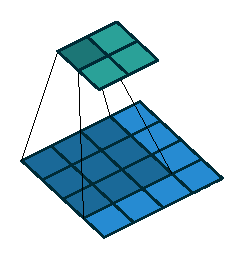
\includegraphics[width=\textwidth]{graphics/neuralnetworks/no_padding_no_strides_00.pdf}
        \caption{}
        \label{fig: Neural networks: no_padding_no_strides_00}
    \end{subfigure}
    \hfill
    \begin{subfigure}[b]{0.24\textwidth}
        \centering
        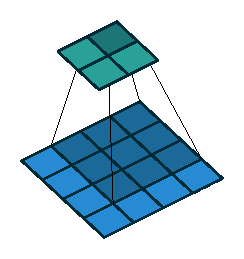
\includegraphics[width=\textwidth]{graphics/neuralnetworks/no_padding_no_strides_01.pdf}
        \caption{}
        \label{fig: Neural networks: no_padding_no_strides_01}
    \end{subfigure}
    \hfill
    \begin{subfigure}[b]{0.24\textwidth}
        \centering
        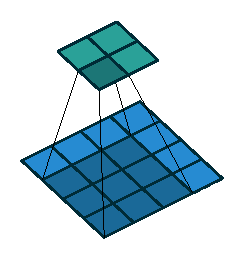
\includegraphics[width=\textwidth]{graphics/neuralnetworks/no_padding_no_strides_02.pdf}
        \caption{}
        \label{fig: Neural networks: no_padding_no_strides_02}
    \end{subfigure}
    \hfill
    \begin{subfigure}[b]{0.24\textwidth}
        \centering
        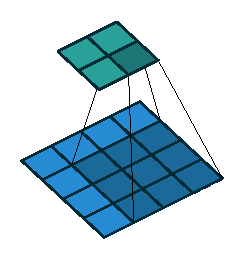
\includegraphics[width=\textwidth]{graphics/neuralnetworks/no_padding_no_strides_03.pdf}
        \caption{}
        \label{fig: Neural networks: no_padding_no_strides_03}
    \end{subfigure}
    \caption{Convolution of a $(4\times4)$ input with a $(3\times3)$ kernel to form a $(2\times2)$ output in four steps. Similarly to the affine transformation of \glspl{FNN}, each output element is a weighted sum of the inputs. The weights are learnable and conversely to \glspl{FNN} they are shared across the input. See also \autoref{fig: Neural networks: numerical_no_padding_no_strides}. Figures due to \cite{Dumoulin2018}.}
    \label{fig: Neural networks: no_padding_no_strides}
\end{figure}

The convolution operation can be formulated as a matrix-vector multiplication. This is demonstrated here by convolution of a $3\times3$ input by a $2\times2$ kernel to form a $2\times2$ feature map. The input is unrolled into columns of the elements acted on by the kernel at each position. The input then forms a symmetric matrix. This is multiplied by the kernel unrolled to a column vector. This can be written as,
\begin{align*}
    \S
    &= \X * \K\\
    &=  \bmat{
            X_{11} & X_{21} & X_{31}\\
            X_{12} & X_{22} & X_{32}\\
            X_{13} & X_{23} & X_{33}
        } * 
        \bmat{
            K_{11} & K_{12}\\
            K_{21} & K_{22}
        }\\
    &=  \bmat{
            X_{11} & X_{12} & X_{21} & X_{22}\\
            X_{12} & X_{13} & X_{22} & X_{23}\\
            X_{21} & X_{22} & X_{31} & X_{32}\\
            X_{22} & X_{23} & X_{32} & X_{33}\\
        }
        \bmat{
            K_{11} \\ K_{12} \\ K_{21} \\ K_{22}
        }_{2\times2}\\
    &=  \bmat{
            K_{11}X_{11} + K_{12}X_{12} + K_{21}X_{21} + K_{22}X_{22}\\
            K_{11}X_{12} + K_{12}X_{13} + K_{21}X_{22} + K_{22}X_{23}\\
            K_{11}X_{21} + K_{12}X_{22} + K_{21}X_{31} + K_{22}X_{32}\\
            K_{11}X_{22} + K_{12}X_{23} + K_{21}X_{32} + K_{22}X_{33}
        }_{2\times2} \ . %\\
    % &=  \bmat{
    %         K_{11}X_{11} + K_{12}X_{12} + K_{21}X_{21} + K_{22}X_{22} &
    %         K_{11}X_{12} + K_{12}X_{13} + K_{21}X_{22} + K_{22}X_{23}\\
    %         K_{11}X_{21} + K_{12}X_{22} + K_{21}X_{31} + K_{22}X_{32} &
    %         K_{11}X_{22} + K_{12}X_{23} + K_{21}X_{32} + K_{22}X_{33}
%        }.
\end{align*}
Note how each feature map element is computed as a weighted sum of the corresponding input elements with the weights defined by the kernel. This is visualized in \autoref{fig: Neural networks: numerical_no_padding_no_strides}. This matrix-vector formulation easily extends to multiple kernels resulting in multiple feature maps by adding additional kernels as columns to the unrolled kernel. Efficient algorithms for computing the convolution is still an active research field \cite{Goodfellow2016}
\begin{figure}[tbp!]
    \begin{subfigure}[b]{0.49\textwidth}
        \centering
        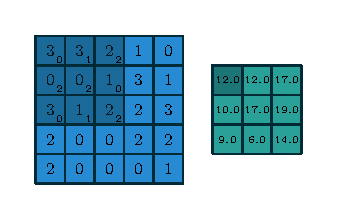
\includegraphics[width=\textwidth]{graphics/neuralnetworks/numerical_no_padding_no_strides_00.pdf}
        \caption{}
        \label{fig: Neural networks: numerical_no_padding_no_strides 1}
    \end{subfigure}
    \hfill
    \begin{subfigure}[b]{0.49\textwidth}
        \centering
        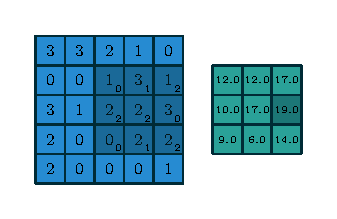
\includegraphics[width=\textwidth]{graphics/neuralnetworks/numerical_no_padding_no_strides_05.pdf}
        \caption{}
        \label{fig: Neural networks: numerical_no_padding_no_strides 2}
    \end{subfigure}
    \caption{Convolution of a $(5\times5)$ input with a $(3\times3)$ kernel to form a $(3\times3)$ output exemplified by two out of a total of nine required steps. It is shown how each feature map element is a weighted sum of the input with the kernel as weights. Figures due to \cite{Dumoulin2018}.}
    \label{fig: Neural networks: numerical_no_padding_no_strides}
\end{figure}

The convolution operation leverages three ideas that separate it from the affine transformation \cite{Goodfellow2016}.
\begin{enumerate}
    \item Sparse connectivity
    \item Parameter sharing
    \item Equivariant representations
\end{enumerate}
These are introduced briefly below.

The \textit{sparse connectivity} arises from each kernel being smaller than the input. Each unit of the feature map is then a function of only part of the input proportional to the kernel size. This also gives rise to the concept of the \textit{local receptive field} which is defined as the range of inputs which are connected to a certain feature map element. The layer that is connected to the input has a receptive field defined by its own kernel size. By stacking convolutional layers, the receptive field increases in size by indirectly connecting to a wider range of inputs through the feature maps of preceeding layers \cite{Goodfellow2016}.

\textit{Parameter sharing} is introduced by letting the kernel act on the entire input image by sliding it across it. Each element in the feature map then depends on learning a kernel that is useful for many locations in the input, This allows a \gls{CNN} to exploit correlations between neighbouring elements in the input. In the case of time series or images this corresponds to exploiting temporal or spatial correlations, irrespective of their specific locations within the input. This is not possible for an \gls{FNN} \cite{Goodfellow2016}. 

The convolution is \textit{equivariant to translations} in its input in the sense that for any translation operation $T$ applied to $\X$ it holds that
\begin{equation}
    T\bra{\X} * \K = T\bra{\X * \K} = \X * T\bra{\K}
\end{equation}
i.e. applying the translation to the input (or kernel) and doing the convolution is equivalent to doing the convolution and then applying the translation to the feature map\footnote{Equivariance differs from invariance. Where equivariance means that output changes in the same way as input does, invariance to a transformation means that output does not change when that transformation is applied to the input. Often, invariance can be obtained fairly easily from equivariance by disregarding the additional information about the input transformation contained in the output \cite{Goodfellow2016}. There has been some discussion of these properties in relation to the newly proposed capsule networks \cite{Sabour2017} as an alternative to \glspl{CNN}.} \cite{Goodfellow2016}.

Beside the input size and kernel size, some other parameters that define the convolution operation are input zero \textit{padding}, the distance between two consecutive positions of the kernel on the input called the \textit{stride}, and \textit{dilation} which controls the distance between the inputs read by the kernel at a single position \cite{Dumoulin2018}.

\begin{figure}[tbp!]
    \begin{subfigure}[b]{0.49\textwidth}
        \centering
        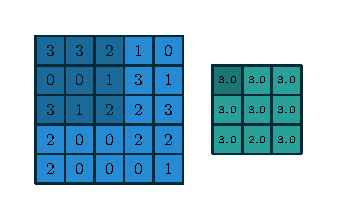
\includegraphics[width=\textwidth]{graphics/neuralnetworks/numerical_max_pooling_00.pdf}
        \caption{}
        \label{fig: Neural networks: numnumerical_max_pooling_00}
    \end{subfigure}
    \hfill
    \begin{subfigure}[b]{0.49\textwidth}
        \centering
        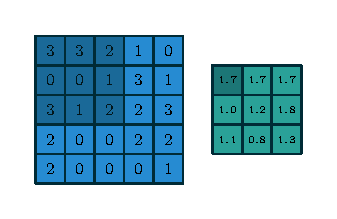
\includegraphics[width=\textwidth]{graphics/neuralnetworks/numerical_average_pooling_00.pdf}
        \caption{}
        \label{fig: Neural networks: numerical_average_pooling_00}
    \end{subfigure}
    \caption{\subref{fig: Neural networks: numnumerical_max_pooling_00} Max- and \subref{fig: Neural networks: numerical_average_pooling_00} average-pooling of a $(5\times5)$ input with a $(3\times3)$ kernel to form a $(3\times3)$. Figures due to \cite{Dumoulin2018}.}
    \label{fig: Neural networks: numerical_pooling}
\end{figure}
In order to shrink the dimension of resulting feature maps, pooling layers are often applied after convolutional layers. Generally, pooling layers summarize a neighbourhood of elements in a feature map into a single element by using some operation. The most widespread type of pooling is max-pooling \cite{Zhou1988, Ranzato2007, Scherer2010}. 
% Here the individual
% \begin{equation}
%     \tilde{S}_{i,j} = \max\cbra{S_{n,m}\mid m\in\bra{i-\frac{n-1}{2},i+\frac{n-1}{2}}, m\in\bra{j-\frac{m-1}{2},j+\frac{m-1}{2}}}
% \end{equation}
When max-pooling is applied to a two dimensional input, each element of the resulting feature map is computed as the maximum element contained within a rectangular pooling kernel applied to the input, similarly to how convolution is computed, by sliding the kernel. Other types of pooling apply a different operation, e.g. averaging, weighted averaging according to distance from center and $L_2$ norm \cite{Goodfellow2016}. Max- and average-pooling are illustrated in \autoref{fig: Neural networks: numerical_pooling}. These pooling operations can make convolution \textit{invariant to translations}, such that output does not change for small translations of the input. When learning multiple kernels in a single convolutional layer and pooling over these, additional invariances, such as rotation invariance, can be learned \cite{Goodfellow2016}.

Conventionally, \glspl{CNN} consist of a series of convolutional layers each followed by a pooling layer and an activation function with the final convolutional layer feature map being flattened and input to an \gls{FNN}, e.g. for classification. In \cite{Lin2013} it was proposed to dispense with the fully connected layers by having the final convolutional layer output a feature map for each of the $K$ classes and averaging them to form a $K$ dimensional vector which is then fed to the softmax activation. Another attempt at making \glspl{CNN} fully convolutional was made in \cite{Long2015}.


\subsection{Recurrent neural networks}
\begin{figure}[tbp!]
    \begin{subfigure}[b]{0.25\textwidth}
        \centering
        \resizebox{!}{3cm}{
            \begin{tikzpicture}[x=1cm, y=1cm, >=stealth, font=\sffamily\scriptsize]
    \tikzstyle{neuron}=[circle, draw, minimum size=.6cm]
    \tikzstyle{Arrow}=[rounded corners=.20cm,thick] % Arrows with rounded corners
    \tikzstyle{cell}=[% For the main box
        rectangle,
        draw,
        rounded corners=1mm,
        very thick,
        minimum width=6mm,
        minimum height=4mm,
        inner sep=3pt
        ]
    % Input node
    \node [neuron] (input) at (0,0) {$\x^\vbra{t}$};
    
    % Recurrent cell
    \node [cell] (cell) at (0,1) {RNN cell};
    
    % Output node
    \node [neuron] (output) at (0,2) {$\h^\vbra{t}$};
    
    % Feedforward arrows
    \draw [->, Arrow] (input) -- (cell);
    \draw [->, Arrow] (cell) -- (output);
    
    % Feedback arrows
    \draw [-, Arrow] (cell.east) -- (1, 1) -- (1, 1.325) -- (0.2, 1.325);
    \draw [<-, Arrow] (cell.west) -- (-1, 1) -- (-1, 1.325) -- (-0.2, 1.325);
\end{tikzpicture}
        }
        \caption{}
        \label{fig: Neural networks: RNN}
    \end{subfigure}
    \hfill
    \begin{subfigure}[b]{0.73\textwidth}
        \centering
        \resizebox{!}{3cm}{
            \newcommand{\empt}[2]{$#1^{\langle #2 \rangle}$}
\begin{tikzpicture}[x=1cm, y=1cm, >=stealth, font=\sffamily\scriptsize]
    \tikzstyle{neuron}=[circle, draw, minimum size=.6cm]
    \tikzstyle{dots}=[draw=none, scale=2, text height=0.333cm, execute at begin node={\color{black}\tiny$\cdots$}]
    \tikzstyle{Arrow}=[rounded corners=.20cm,thick] % Arrows with rounded corners
    \tikzstyle{cell}=[% For the main box
        rectangle,
        draw,
        rounded corners=1mm,
        very thick,
        minimum width=6mm,
        minimum height=4mm,
        inner sep=3pt
        ]
    
    % Input nodes
    \node [neuron] (input1) at (0,0) {\empt{\x}{1}};
    \node [neuron] (input2) at (2,0) {\empt{\x}{2}};
    \node [neuron] (inputT) at (6,0) {\empt{\x}{T}};
    
    % Recurrent cells
    \node [cell] (cell1) at (0,1) {RNN cell};
    \node [cell] (cell2) at (2,1) {RNN cell};
    \node [cell] (cellT) at (6,1) {RNN cell};
    
    % Hidden nodes
    \node [neuron] (hidden0) at (-1.5,1) {\empt{\h}{0}};
    \node [neuron] (hidden1) at (0,2) {\empt{\h}{1}};
    \node [neuron] (hidden2) at (2,2) {\empt{\h}{2}};
    \node [neuron] (hiddenT) at (6,2) {\empt{\h}{T}};
    
    % Dots
    \node [neuron, draw=none, scale=2] (dots1) at (4,1) {\tiny$\dots$};
    
    % Hidden to cell to cell ... to cell
    \draw [->, Arrow] (hidden0) -- (cell1);
    \draw [->, Arrow] (cell1) -- (cell2);
    \draw [->, Arrow] (cell2) -- (dots1);
    \draw [->, Arrow] (dots1) -- (cellT);
    
    % Input to cell to hidden
    \draw [->, Arrow] (input1) -> (cell1) -- (hidden1);
    \draw [->, Arrow] (input2) -> (cell2) -- (hidden2);
    \draw [->, Arrow] (inputT) -> (cellT) -- (hiddenT);
\end{tikzpicture}
        }
        \caption{}
        \label{fig: Neural networks: RNN unrolled}
    \end{subfigure}
    \caption{\subref{fig: Neural networks: RNN} Illustration of the feedback loop in a basic \gls{RNN}. Without the feedback this would have been an ordinary \gls{FNN}. \subref{fig: Neural networks: RNN unrolled} The same \gls{RNN} but unrolled in time. Each recurrent cell applies the same set of operations recurrently on each input element and updated hidden state. Figures inspired by \cite{Olah2015}.}
    \label{fig: Neural networks: RNNs}
\end{figure}
\Glspl{RNN} \cite{Rumelhart1986} are a type of neural networks specialized for processing sequential data of variable length. 
Given an input sequence $\cbra{\x^\vbra{t}}_{t=1}^{T}=\cbra{\x^\vbra{1}, \x^\vbra{2}, \dots, \x^\vbra{T}}$ of length $T$ an \gls{RNN} recurrently applies the same series of operations to each sequence time step, $\x^\vbra{t}$, starting from one end or both ends if the \gls{RNN} is \textit{bidirectional}. The power of \glspl{RNN} lie in the ability to compute some hidden state which changes depending on the entire history of seen sequence vectors. This works as a kind of memory.

An \gls{RNN} can be represented as a computational graph with a feedback loop as in \autoref{fig: Neural networks: RNN}. There, the entire sequence $\x$ is the input and the RNN cell outputs the hidden state $\h$. Such a graph can be unrolled to the length of the input sequence as seen in \autoref{fig: Neural networks: RNN unrolled}. It is then clear how the input sequence is read element by element while the hidden state is updated. The hidden state sequence may have a length different from the length of the input sequence. A length of $1$ for the hidden state sequence is typically used for classification. There is no requirement that a hidden state must be output whenever a input is read. In fact, an \gls{RNN} can consist of an encoder which first reads the input sequence and a decoder which then constructs the output.
\begin{figure}[tbp!]
    \centering
    \newcommand{\empt}[2]{$#1^{\langle #2 \rangle}$}
\begin{tikzpicture}[
    % GLOBAL CFG
    font=\sffamily\scriptsize,
    >=LaTeX,
    % Styles
    cell/.style={% For the main box
        rectangle, 
        rounded corners=5mm, 
        draw,
        very thick,
        },
    vector/.style={% For external inputs and outputs
        circle,
        draw,
        line width = .75pt,
        minimum width=1cm,
        inner sep=1pt,
        },
    gate/.style={% For internal inputs
        rectangle,
        draw,
        minimum width=4mm,
        minimum height=3mm,
        inner sep=1pt
        },
    mylabel/.style={% something new that I have learned
        font=\scriptsize\sffamily
        },
    ArrowC1/.style={% Arrows with rounded corners
        rounded corners=.25cm,
        thick,
        }
    ]

    % Cell
    \node [cell, minimum height=4cm, minimum width=6cm] at (0,0){} ;
    
    % Inputs
    \node[vector, label={[mylabel]Hidden}] (h) at (-4,1.5) {\empt{\h}{t-1}};
    \node[vector, label={[mylabel]left:Input}] (x) at (-2.5,-3) {\empt{\x}{t}};
    
    % Outputs
    \node[vector, label={[mylabel]Hidden}] (h2) at (4,1.5) {\empt{\h}{t}};
    \node[vector, label={[mylabel]left:Hidden}] (h22) at (2.5,3) {\empt{\h}{t}};
    
    \node [gate, minimum width=1cm] (hiddengate) at (0,0) {tanh};

    % Coordinates
    \coordinate(hiddenbend) at (-2,1.5);
    \coordinate(inputbend) at (-2.5,-1);
    \coordinate(hxjoin) at (-2,-1);
    \coordinate(bendbelowtanh) at (0,-1);
    \coordinate(bendabovetanh) at (0,1.5);
    \coordinate(hiddensplit) at (2.5,1.5);

    % Arrows
    \draw [ArrowC1] (h) -- (hiddenbend) -- (hxjoin) -- (bendbelowtanh) -- (hiddengate);
    \draw [ArrowC1] (x) -- (inputbend) -- (hxjoin)--++(0.5,0);
    \draw [ArrowC1] (hiddengate) -- (bendabovetanh) -- (h2);
    \draw [ArrowC1] (hiddensplit)++(-0.5,0) -- (hiddensplit) -- (h22);
\end{tikzpicture}
    \caption{Layout of the basic recurrent cell. Due to the small gradients of the $\tanh$, this cell is often not able to propagate error signals far enough back in time to learn long term dependencies. Figure inspired by \cite{Olah2015}.}
    \label{fig: Neural networks: RNN cell}
\end{figure}
The RNN cell in \autoref{fig: Neural networks: RNNs} represents the operation applied to the input $\x^\vbra{t}$ given the hidden state $\h^\vbra{t-1}$. Beside the network architecture, the operations specified by this recurrent cell are what defines the \gls{RNN}. A basic \gls{RNN} has a cell defined by a single fully connected layer which acts on the (concatenated) input and hidden states.
\begin{equation}
    \h^\vbra{t} = \tanh\pa{\W_{hh}\h^\vbra{t-1}+\W_{hx}\x^\vbra{t}+\b_h}
\end{equation}
This cell is illustrated in \autoref{fig: Neural networks: RNN cell}. In \autoref{fig: Neural networks: RNN cell} and the following ones, nodes represent vectors while lines and arrows illustrate the flow of these. Two lines merging denotes the concatenation of the two corresponding vectors while the splitting of a line represents the corresponding vector being copied. Square boxes represent a single layered \gls{FNN}, i.e. an affine transformation of the input, and the text inside denotes the used nonlinearity.
Due to the problem of \textit{vanishing gradients} this type of \gls{RNN} is not able to learn long term dependencies and is tricky to train overall. This problem arises since the gradients of the $\tanh$ activation are constrained within $(0,1]$ and tend to zero for large and small inputs as previously described. Recurrently multiplying many small gradients results in increasingly smaller gradients the further back in time they are propagated.

\begin{figure}[tbp!]
    \centering
    \newcommand{\empt}[2]{$#1^{\langle #2 \rangle}$}
\begin{tikzpicture}[
    % GLOBAL CFG
    font=\sffamily\scriptsize,
    >=LaTeX,
    % Styles
    cell/.style={% For the main box
        rectangle, 
        rounded corners=5mm, 
        draw,
        very thick,
        },
    operator/.style={%For operators like +  and  x
        circle,
        draw,
        inner sep=0pt,
        minimum height =.2cm,
        },
    function/.style={%For functions
        ellipse,
        draw,
        inner sep=1pt
        },
    vector/.style={% For external inputs and outputs
        circle,
        draw,
        line width = .75pt,
        minimum width=1cm,
        inner sep=1pt,
        },
    gate/.style={% For internal inputs
        rectangle,
        draw,
        minimum width=4mm,
        minimum height=3mm,
        inner sep=1pt
        },
    mylabel/.style={% something new that I have learned
        font=\scriptsize\sffamily
        },
    ArrowC1/.style={% Arrows with rounded corners
        rounded corners=.25cm,
        thick,
        },
    ArrowC2/.style={% Arrows with big rounded corners
        rounded corners=.5cm,
        thick,
        },
    ]

    % Start drawing the thing...    
    % Draw the cell: 
    \node [cell, minimum height =4cm, minimum width=6cm] at (0,0){} ;

    % Draw inputs named
    \node [gate] (forgetgate) at (-2,-0.75) {$\sigma$};
    \node [gate] (inputgate) at (-1.5,-0.75) {$\sigma$};
    \node [gate, minimum width=1cm] (cellgate) at (-0.5,-0.75) {tanh};
    \node [gate] (outputgate) at (0.5,-0.75) {$\sigma$};

   % Draw operators
    \node [operator] (mux1) at (-2,1.5) {$\times$};
    \node [operator] (add1) at (-0.5,1.5) {$+$};
    \node [operator] (mux2) at (-0.5,0) {$\times$};
    \node [operator] (mux3) at (1.5,0) {$\times$};
    \node [function] (tanh1) at (1.5,0.75) {tanh};

    % Draw External inputs? named as basis c,h,x
    \node[vector, label={[mylabel]Cell}] (c) at (-4,1.5) {\empt{\c}{t-1}};
    \node[vector, label={[mylabel]Hidden}] (h) at (-4,-1.5) {\empt{\h}{t-1}};
    \node[vector, label={[mylabel]left:Input}] (x) at (-2.5,-3) {\empt{\x}{t}};

    % Draw External outputs? named as basis c2,h2,h22
    \node[vector, label={[mylabel]Cell}] (c2) at (4,1.5) {\empt{\c}{t}};
    \node[vector, label={[mylabel]Hidden}] (h2) at (4,-1.5) {\empt{\h}{t}};
    \node[vector, label={[mylabel]left:Hidden}] (h22) at (2.5,3) {\empt{\h}{t}};

    % Start connecting all with arrows.
    % Intersections and displacements are used. 
    % Drawing arrows    
    \draw [ArrowC1] (c) -- (mux1) -- (add1) -- (c2);

    % Inputs
    \draw [ArrowC2] (h) -| (outputgate);
    \draw [ArrowC1] (h -| forgetgate)++(-0.5,0) -| (forgetgate); 
    \draw [ArrowC1] (h -| inputgate)++(-0.5,0) -| (inputgate);
    \draw [ArrowC1] (h -| cellgate)++(-0.5,0) -| (cellgate);
    \draw [ArrowC1] (x) -- (x |- h) -| (cellgate);

    % Internal
    \draw [->, ArrowC2] (forgetgate) -- node[right, near end]{\empt{\f}{t}} (mux1);
    \draw [->, ArrowC2] (inputgate) |- node{\empt{\i}{t}} (mux2);
    \draw [->, ArrowC2] (cellgate) -- node[right]{\empt{\tilde{\c}}{t}} (mux2);
    \draw [->, ArrowC2] (outputgate) |- node{\empt{\o}{t}} (mux3);
    \draw [->, ArrowC2] (mux2) -- (add1);
    \draw [->, ArrowC1] (add1 -| tanh1)++(-0.5,0) -| (tanh1);
    \draw [->, ArrowC2] (tanh1) -- (mux3);

    % Outputs
    \draw [-, ArrowC2] (mux3) |- (h2);
    \draw (c2 -| h22) ++(0,-0.1) coordinate (i1);
    \draw [-, ArrowC2] (h2 -| h22)++(-0.5,0) -| (i1);
    \draw [-, ArrowC2] (i1)++(0,0.2) -- (h22);
\end{tikzpicture}

    \caption{Layout of the \gls{LSTM} cell. The cell state $\c^\vbra{t}$ effectively propogates gradients far backwards in time since it is never squashed in an activation function. The hidden state and input are concatenated and used to compute forget, input and output gates along with a proposed new cell state. Figure inspired by \cite{Olah2015}.}
    \label{fig: Neural networks: LSTM cell} 
\end{figure}
A much more successful recurrent cell structure is the \gls{LSTM} cell \cite{Hochreiter1997} illustrated in \autoref{fig: Neural networks: LSTM cell}. Here, small interior circular nodes represent elementwise operations by the shown operator and elliptical nodes indicate elementwise application of a function.. To avoid the ing gradients problem this cell introduces a cell state $\c^\vbra{t}$ which passes through time without being squashed in activations. It is instead modified multiplicatively and additively by the outputs of certain gates. The gates are designed to learn which parts of the previous cell state to \textit{forget}, which parts of the input and hidden state to \textit{input} to the new cell state and which new hidden state to \textit{output},
\begin{subequations}
    \begin{align}
        \f^\vbra{t} &= \sigma\pa{\W_{fh}\h^\vbra{t-1}+\W_{fx}\x^\vbra{t}+\b_f}\\
        \i^\vbra{t} &= \sigma\pa{\W_{ih}\h^\vbra{t-1}+\W_{ix}\x^\vbra{t}+\b_i}\\
        \o^\vbra{t} &= \sigma\pa{\W_{oh}\h^\vbra{t-1}+\W_{ox}\x^\vbra{t}+\b_o} \ .
    \end{align}
\end{subequations}
The new cell state is computed from a proposed cell state $\tilde{\c}^\vbra{t}$ and the forget and input gates  $\f^\vbra{t}$ and $\i^\vbra{t}$. The new hidden state is computed from the output gate $\o^\vbra{t}$ and the new cell state,
\begin{subequations}
    \begin{align}
        \tilde{\c}^\vbra{t} &= \tanh\pa{\W_{ch}\h^\vbra{t-1}+\W_{cx}\x^\vbra{t}+\b_c}\\
        \c^\vbra{t} &= \f^\vbra{t}\odot\c\vbra{t-1}+\i^\vbra{t}\odot\tilde{\c}^\vbra{t}\\
        \h^\vbra{t} &= \o^\vbra{t}\odot\tanh\pa{\c^\vbra{t}} \ .
    \end{align}
\end{subequations}

There exists a number of variations on the design of the \gls{LSTM} cell. One such variation includes peephole connections \cite{Gers2000} that allows the gates to see the cell state. This peephole \gls{LSTM} is shown in \autoref{fig: Neural networks: Peephole LSTM cell}. Other noteworthy variations include the \gls{LSTM} with coupled forget and input gates and the \gls{GRU} \cite{Cho2014a} which simplifies the \gls{LSTM} by using a joint cell and hidden state and only two gates, update and reset.
\begin{figure}[tbp!]
    \centering
    \newcommand{\empt}[2]{$#1^{\langle #2 \rangle}$}
\begin{tikzpicture}[
    % GLOBAL CFG
    font=\sffamily\scriptsize,
    >=LaTeX,
    % Styles
    cell/.style={% For the main box
        rectangle, 
        rounded corners=5mm, 
        draw,
        very thick,
        },
    operator/.style={%For operators like +  and  x
        circle,
        draw,
        inner sep=0pt,
        minimum height =.2cm,
        },
    function/.style={%For functions
        ellipse,
        draw,
        inner sep=1pt
        },
    vector/.style={% For external inputs and outputs
        circle,
        draw,
        line width = .75pt,
        minimum width=1cm,
        inner sep=1pt,
        },
    gate/.style={% For internal inputs
        rectangle,
        draw,
        minimum width=4mm,
        minimum height=3mm,
        inner sep=1pt
        },
    mylabel/.style={% something new that I have learned
        font=\scriptsize\sffamily
        },
    ArrowC1/.style={% Arrows with rounded corners
        rounded corners=.25cm,
        thick,
        },
    ArrowC2/.style={% Arrows with big rounded corners
        rounded corners=.5cm,
        thick,
        },
    ArrowC3/.style={% Arrows with rounded corners
        rounded corners=.20cm,
        thick,
        },
    ]

    % Start drawing the thing...    
    % Draw the cell: 
    \node [cell, minimum height=4cm, minimum width=6cm] at (0,0){} ;

    % Draw inputs named ibox#
    \node [gate] (forgetgate) at (-2,-0.75) {$\sigma$};
    \node [gate] (inputgate) at (-1.5,-0.75) {$\sigma$};
    \node [gate, minimum width=1cm] (cellgate) at (-0.5,-0.75) {tanh};
    \node [gate] (outputgate) at (0.5,-0.75) {$\sigma$};

    % Draw operators   named mux# , add# and func#
    \node [operator] (mux1) at (-2,1.5) {$\times$};
    \node [operator] (add1) at (-0.5,1.5) {$+$};
    \node [operator] (mux2) at (-0.5,0) {$\times$};
    \node [operator] (mux3) at (1.5,0) {$\times$};
    \node [function] (tanh1) at (1.5,0.75) {tanh};

    % Draw External inputs? named as basis c,h,x
    \node[vector, label={[mylabel]Cell}] (c) at (-4,1.5) {\empt{\c}{t-1}};
    \node[vector, label={[mylabel]Hidden}] (h) at (-4,-1.5) {\empt{\h}{t-1}};
    \node[vector, label={[mylabel]left:Input}] (x) at (-2.5,-3) {\empt{\x}{t}};

    % Draw External outputs? named as basis c2,h2,h22
    \node[vector, label={[mylabel]Cell}] (c2) at (4,1.5) {\empt{\c}{t}};
    \node[vector, label={[mylabel]Hidden}] (h2) at (4,-1.5) {\empt{\h}{t}};
    \node[vector, label={[mylabel]left:Hidden}] (h22) at (2.5,3) {\empt{\h}{t}};

    % Start connecting all with arrows.
    % Intersections and displacements are used. 
    % Drawing arrows
    \draw [ArrowC1] (c) -- (mux1) -- (add1) -- (c2);

    % Inputs
    \draw [ArrowC2] (h) -| (outputgate);
    \draw [ArrowC1] (h -| forgetgate)++(-0.5,0) -| (forgetgate); 
    \draw [ArrowC1] (h -| inputgate)++(-0.5,0) -| (inputgate);
    \draw [ArrowC1] (h -| cellgate)++(-0.5,0) -| (cellgate);
    \draw [ArrowC1] (x) -- (x |- h) -| (cellgate);

    % Internal
    \draw [->, ArrowC2] (forgetgate) -- node[right, near end]{\empt{\f}{t}} (mux1);
    \draw [->, ArrowC2] (inputgate) |- node{\empt{\i}{t}} (mux2);
    \draw [->, ArrowC2] (cellgate) -- node[right]{\empt{\tilde{\c}}{t}} (mux2);
    \draw [->, ArrowC2] (outputgate) |- node{\empt{\o}{t}} (mux3);
    \draw [->, ArrowC2] (mux2) -- (add1);
    \draw [->, ArrowC1] (add1 -| tanh1)++(-0.5,0) -| (tanh1);
    \draw [->, ArrowC2] (tanh1) -- (mux3);

    % Outputs
    \draw [-, ArrowC2] (mux3) |- (h2);
    \draw (c2 -| h22) ++(0,-0.1) coordinate (i1);
    \draw [-, ArrowC2] (h2 -| h22)++(-0.5,0) -| (i1);
    \draw [-, ArrowC2] (i1)++(0,0.2) -- (h22);
    
    % Peepholes
    % Cell to forget gate
    \draw [ArrowC1] (-2.7,1.5) -- (-2.7,-1.25) -- (-2,-1.25) coordinate(tmp) -- (forgetgate);
    % Below forget gate to input gate
    \draw [ArrowC1] (tmp)++(-0.3,0) -- (-2.075,-1.25); %(tmp)++(-0.2,0);
    \draw [ArrowC1] (-1.925,-1.25) -- (-1.5,-1.25) -- (inputgate);
    % Cell to output gate
    \draw [ArrowC3] (0.075,1.5) -- (0.075,-1.25) -- (0.5,-1.25) -- (outputgate.south);
\end{tikzpicture}
    \caption{Layout of the peephole variant of the \gls{LSTM} cell. Compared to the \gls{LSTM}, gates are allowed acces to the cell state when computing their output. This is just one of many variants that have arisen of the \gls{LSTM}. Figure inspired by \cite{Olah2015}.}
    \label{fig: Neural networks: Peephole LSTM cell}
\end{figure}

%!TEX root = ../Thesis.tex

\section{Training neural networks}
\subsection{Error functions}
Various error functions for different classes of problems can be derived by following the maximum likelihood approach. For a network $\y(\x,\w)$ with parameters denoted by $\w$, the approach is as follows. First, the assumed distribution of targets given input $\x$ and network, $p(\t|\x,\w)$, is defined. Then its likelihood $p(\T|\X,\w)$ is formed for a batch of inputs and targets, $\X=\cbra{\x_i \mid i\in\mathcal{B}}$, $\T=\cbra{\t_i \mid i\in\mathcal{B}}$, where $\mathcal{B}$ is a batch of indices to the dataset $\mathcal{D}$. Finally the negative logarithm of the likelihood is minimized w.r.t. $\w$.

In deep learning it is common to derive a loss function from the log-likelihood and instead minimize that \cite{Bishop2006}. The error function should take the form of a sum over individual error terms, each of which must be a function of the network parameters \cite{Nielsen2015},
\begin{equation}\label{eq: Neural networks: Error as a sum over individual terms}
    E(\w) = \sum_{i\in\mathcal{B}} E_i \ .
\end{equation}
The following will present some common error functions.

An assumed Gaussian distribution of targets with shared noise variance, $p(\t|\x,\w)=\mathcal{N}(\t|\y(\x,\w),\sigma^2\I)$, results in a regression problem and the \gls{MSE}
\begin{equation}
    E_\text{MSE}(\w) = \frac{1}{2}\sum_{i\in\mathcal{B}} \norm{\y_i-\t_i}^2_2
\end{equation}
where the division by $\size{\mathcal{B}}$ has been neglected since it does not affect minimization. The noise variance $\sigma^2$ can be found from the regular \gls{MLE}.

For Bernoulli distributed targets, $t\in\cbra{0,1}$, the predictions are scalar, $y\in\bra{0,1}$, and $p(t|\x,\w)=y(\x,\w)^t\pa{1-y(\x,\w)}^{1-t}$. The result is the binary \gls{CEL},
\begin{equation}
    E_\text{BCEL}(\w) = -\sum_{i\in\mathcal{B}} t_i\log y_i + \pa{1-t_i}\log\pa{1-y_i} \ .
\end{equation}

With $K$ separate binary classifications between independent classes, the target distribution can be modelled by $p(\t|\x,\w)=\prod_{k=1}^K y_k(\x,\w)^{t_k}\pa{1-y_k(\x,\w)}^{1-t_k}$ where a label $t_k\in\cbra{0,1}$ is associated with each of the $K$ classes. The resulting loss is the ``separate" \gls{CEL}
\begin{equation}
    E_\text{SCEL}(\w) = -\sum_{i\in\mathcal{B}}\sum_{k=1}^K t_{ik}\log y_{ik} + \pa{1-t_{ik}}\log\pa{1-y_{ik}} \ .
\end{equation}
with $y_{ik}=y_k(\x_i,\w)$.

If the $K$ classes are mutually exclusive then $p(t|\x,\w)$ is the categorical, or multinoulli, distribution which can be written as $p(\t|\x,\w)=\prod_{k=1}^K \y_k(\x,\w)^{t_k}$ using a one-hot encoding of the targets $\t$. The result is the categorical \gls{CEL}
\begin{equation}
    E_\text{CCEL}(\w) = -\sum_{i\in\mathcal{B}}\sum_{k=1}^K t_{ik}\log y_{ik} \ .
\end{equation}

\subsection{The canonical link}
It should be noted that the choice of final layer activation is intimately connected to the chosen error function through the so-called \textit{canonical link function}. When combining an error function with the corresponding canonical link function as activation, the gradient of a single contribution to the error w.r.t. the output layer hidden units $\z^{\bra{L}}$ takes the form of a signed error,
\begin{equation}
    \pderiv{E_i}{\z_i^{\bra{L}}} = \pderiv{E_i}{\a_i^{\bra{L}}}\pderiv{\a_i^\bra{L}}{\z_i^\bra{L}} = \y_i-\t_i \ .
\end{equation}
The canonical activation for the \gls{MSE} loss is the identity function, i.e. the output units are simply linear. This can easily be seen by setting $\a^{\bra{L}}=\z^{\bra{L}}$. Then 
\begin{equation*}
    \pderiv{\a^\bra{L}}{\z^\bra{L}}=\I
\end{equation*}
and by definition of $\y$ and the \gls{MSE},
\begin{align*}
    \pderiv{E_i}{\z^{\bra{L}}}
    &= \pderiv{E_i}{\a^{\bra{L}}}\\
    &= \pderiv{E_i}{\y}\\
    %&= \pderiv{}{\y} \bra{\frac{1}{2}(\y-\t)\transpose(\y-\t)}\\
    &= \pderiv{}{\y}\norm{\y-\t}_2^2\\
    &= \y-\t \ ,
\end{align*}
ignoring the $i$ subscript on $\y, \t, \z^\bra{L}$ and $\a^\bra{L}$ for simplicity.
For the binary and $K$ class separate binary \gls{CEL} the canonical activation is the sigmoid while for the multiclass \gls{CEL} it is the softmax \cite{Bishop2006}. These relation won't be derived here. When applying the canonical link for the error functions above, the loss is also sometimes referred to as the \gls{NLL} loss.


\subsection{Backpropagation}
The predominant method for training of neural networks is the \textit{backpropagation} algorithm. Much as for the perceptron, an error function is defined and the network is optimized to minimize this error. The gradient of the error function w.r.t. all learnable parameters of the network is computed and used to adjust these in the direction that minimizes error.

The backpropagation algorithm is at its core a serial application of the chain rule of calculus. As such it requires a differentiable network model in that the applied transformations and nonlinearities must be differentiable. It also requires a differentiable error function as discussed above \cite{Nielsen2015}. A model satisfying these requirements is sometimes called \textit{end-to-end differentiable}.

\subsubsection{Backpropagation in feedforward neural networks}
Consider an \gls{FNN}. By the chain rule, the gradient of the loss w.r.t. to the hidden units of any layer $l$ can be written as
\begin{equation}\label{eq: Neural networks: Backpropagation in FNN to arbitrary depth hidden unit}
    \pderiv{E_i}{\z^\bra{l}} = 
    \underbrace{
        \underbrace{
            \underbrace{
                \pderiv{E_i}{\a^\bra{L}}\pderiv{\a^\bra{L}}{\z^\bra{L}}
            }_{\deltab^\bra{L}}
            \pderiv{\z^\bra{L}}{\a^\bra{L-1}}\pderiv{\a^\bra{L-1]}}{\z^\bra{L-1}}
        }_{\deltab^\bra{L-1}}
        \dots
        \pderiv{\z^\bra{l+1}}{\a^\bra{l}} \pderiv{\a^\bra{l}}{\z^\bra{l}}
    }_{\deltab^\bra{l}}
\end{equation}
where the accumulated \textit{error signals}, $\deltab^\bra{l}$, have been defined as shown. These are useful for making notation more compact and illustrating the symmetry of backpropagation. One should note that the derivative of a scalar by a vector is a vector (gradient), the derivative of a vector by a vector is a matrix (Jacobian) and the derivative of a scalar by a matrix is a matrix.
It is important to be mindful of dimensions while taking matrix and vector derivatives.
Except for the output layer the chain rule can be applied sequentially all through the \gls{FNN} by repeating the 
\begin{equation*}
    \dots\pderiv{\z^\bra{l+1}}{\a^\bra{l}} \pderiv{\a^\bra{l}}{\z^\bra{l}}\dots
\end{equation*}
pattern. The gradient w.r.t. any learnable parameter can then be found by finally appending the derivative of the appropriate hidden unit with respect to that parameter\footnote{This is of course assuming that the learnable parameter resides in the hidden unit transformation. If for instance the activation function has some learnable parameter, the appropriate derivative of $\a^\bra{l}$ is simply appended the $\pderiv{\z^\bra{l+1}}{\a^\bra{l}}$ term instead.}.

One can note that $\deltab^\bra{L}$ will equal $\y-\t$ in case the canonical link activation is used. 
One can also note that the $\pderiv{\z^\bra{l+1}}{\a^\bra{l}}$ terms are derivatives of the $l$'th layer affine transformation w.r.t. its input and that the $\pderiv{\a^\bra{l}}{\z^\bra{l}}$ terms are the derivatives of the $l$'th layer activation function w.r.t. its inputs.

For any activation applied elementwise to an $H_l$-dimensional hidden unit, the $\pderiv{\a^\bra{l}}{\z^\bra{l}}$ term can be seen to be a diagonal matrix. This can be computed as follows.
\begin{align}
    \pderiv{\a^\bra{l}}{\z^\bra{l}}
    &= \pderiv{}{\z^\bra{l}}\bra{\varphi_l\pa{\z^\bra{l}}} = \pderiv{}{\z^\bra{l}}\bmat{\varphi_l\pa{z_1^\bra{l}}\\\varphi_l\pa{z_2^\bra{l}}\\\vdots\\\varphi_l\pa{z_{H_l}^\bra{l}}}\nonumber
    \shortintertext{which is the Jacobian matrix,}
    \pderiv{\a^\bra{l}}{\z^\bra{l}}
    &= \bmat{
        \pderiv{\varphi_l\pa{z_1^\bra{l}}}{z_1^\bra{l}} & \dots & \pderiv{\varphi_l\pa{z_1^\bra{l}}}{z_H^\bra{l}} \\ 
        \vdots & \ddots & \vdots \\
        \pderiv{\varphi_l\pa{z_{H_l}^\bra{l}}}{z_1^\bra{l}} & \dots & \pderiv{\varphi_l\pa{z_{H_l}^\bra{l}}}{z_{H_l}^\bra{l}}
    },\nonumber
    \shortintertext{which reduces to}
    \pderiv{\a^\bra{l}}{\z^\bra{l}}
    &= \bmat{
        \varphi_l'\pa{z_1^\bra{l}} & \dots & 0 \\ 
        \vdots & \ddots & \vdots \\
        0 & \dots & \varphi_l'\pa{z_{H_l}^\bra{l}}
    }
    = \text{diag}\pa{\varphi_l'\pa{\z^\bra{l}}} \ .\label{eq: Neural networks: Gradient of activation function applied elementwise to hidden unit}
\end{align}
% \begin{align}\label{eq: Neural networks: Gradient of activation function applied elementwise to hidden unit}
%     \pderiv{\a^\bra{l}}{\z^\bra{l}}
%     &= \pderiv{}{\z^\bra{l}}\bra{\varphi_l\pa{\z^\bra{l}}}\nonumber\\
%     % &= \pderiv{}{\z^\bra{l}}\bra{\varphi_l\pa{\bmat{z_1^\bra{l}\\z_2^\bra{l}\\\vdots\\z_H^\bra{l}}}}\nonumber\\
%     &= \pderiv{}{\z^\bra{l}}\bmat{\varphi_l\pa{z_1^\bra{l}}\\\varphi_l\pa{z_2^\bra{l}}\\\vdots\\\varphi_l\pa{z_{H_l}^\bra{l}}}\nonumber\\
%     &= \bmat{
%         \pderiv{\varphi_l\pa{z_1^\bra{l}}}{z_1^\bra{l}} & \dots & \pderiv{\varphi_l\pa{z_1^\bra{l}}}{z_H^\bra{l}} \\ 
%         \vdots & \ddots & \vdots \\
%         \pderiv{\varphi_l\pa{z_{H_l}^\bra{l}}}{z_1^\bra{l}} & \dots & \pderiv{\varphi_l\pa{z_{H_l}^\bra{l}}}{z_{H_l}^\bra{l}}
%     } \nonumber \\
%     &= \bmat{
%         \varphi_l'\pa{z_1^\bra{l}} & \dots & 0 \\ 
%         \vdots & \ddots & \vdots \\
%         0 & \dots & \varphi_l'\pa{z_{H_l}^\bra{l}}
%     } \nonumber \\
%     % &=  \text{diag}\pa{\varphi_l'\pa{\bmat{
%     % z_1^\bra{l} \\ 
%     % \vdots \\
%     % z_H^\bra{l} }}} \nonumber \\
%     &=  \text{diag}\pa{\varphi_l'\pa{\z^\bra{l}}}.
% \end{align}
Thus, the derivative of the activation is applied elementwise to the hidden unit and arranged in a diagonal matrix.

Since multiplication of a vector by a diagonal matrix effectively multiplies each element of the vector by the corresponding diagonal element, the output layer error signal can be written as
\begin{align}\label{eq: Neural networks: FNN Backpropagation 1 delta L}
    \deltab^\bra{L}
    &= \pderiv{E_i}{\a^\bra{L}}\pderiv{\a^\bra{L}}{\z^\bra{L}}\nonumber\\
    &= \pderiv{E_i}{\a^\bra{L}}\text{diag}\pa{\varphi_L'\pa{\z^\bra{L}}}\nonumber\\
    &= \pderiv{E_i}{\a^\bra{L}}\odot\varphi_L'\pa{\z^\bra{L}}
\end{align}
where $\odot$ denotes the Hadamard product and $\pderiv{E_i}{\a^\bra{L}}$ could equivalently be written as $\nabla_{\a^\bra{L}}E_i$ since it is the gradient of $E_i$. As activations are computed elementwise from hidden units, there are as many elements in the gradient of $E_i$ w.r.t $\a^\bra{L}$ as there are in $\varphi_L'\pa{\z^\bra{L}}$ and the dimensions match in the elementwise product. The result for the canonical link still holds and $\deltab^\bra{L}$ simplifies to $\y-\t$ for such an output activation.

Using the forward propagation equations for a single \gls{FNN} layer \eqref{eq: Neural networks: Feedforward neural network forward pass for l'th layer} and the previous result for the derivative of an elementwise applied activation function \eqref{eq: Neural networks: Gradient of activation function applied elementwise to hidden unit}, the error signal of the $l$'th layer, $\deltab^\bra{l}$ can be written in terms of the error signal of the next layer, $\deltab^\bra{l+1}$. By \eqref{eq: Neural networks: Backpropagation in FNN to arbitrary depth hidden unit},
\begin{align}\label{eq: Neural networks: FNN Backpropagation 2 delta l}
    \deltab^\bra{l}
    &= \deltab^\bra{l+1}\pderiv{\z^\bra{l+1}}{\a^\bra{l}} \pderiv{\a^\bra{l}}{\z^\bra{l}}\nonumber\\
    &= \deltab^\bra{l+1}\pderiv{}{\a^\bra{l}}\bra{\W^\bra{l+1}\a^\bra{l}+\b^\bra{l+1}} \odot\varphi_l'\pa{\z^\bra{l}}\nonumber\\
    &= \W^{\bra{l+1}\transpose} \deltab^\bra{l+1} \odot\varphi_l'\pa{\z^\bra{l}} \ , \quad l\in\bra{1,L-1} \ .
\end{align}
This equation gives the means to efficiently backpropagate error signals through the computational graph of an \gls{NN}. The error signal into layer $l$ has the same dimensionality as the number of hidden units in that layer. Therefore, the matrix-vector product $\W^{\bra{l+1}\transpose} \deltab^\bra{l+1}$ will have valid dimensions. The following elementwise multiplication by $\varphi_l'\pa{\z^\bra{l}}$ matches the number of rows in $\W^{\bra{l+1}\transpose}$ since $\z^\bra{l}$ has dimensionality of the number of columns in $\W^\bra{l+1}$ by \eqref{eq: Neural networks: Feedforward neural network forward pass for l'th layer}.

For the weight of the $l$'th layer, the gradient is computed by \eqref{eq: Neural networks: Backpropagation in FNN to arbitrary depth hidden unit} as follows,
\begin{align}\label{eq: Neural networks: FNN Backpropagation 3 W}
    \pderiv{E_i}{\W^\bra{l}}
    &= \overbrace{
            \pderiv{E}{\a^\bra{L}}\pderiv{\a^\bra{L}}{\z^\bra{L}}
            \pderiv{\z^\bra{L}}{\a^\bra{L-1}}\pderiv{\a^\bra{L-1]}}{\z^\bra{L-1}}
            \dots
            \pderiv{\z^\bra{l+1}}{\a^\bra{l}} \pderiv{\a^\bra{l}}{\z^\bra{l}}
        }^{\deltab^\bra{l}} \pderiv{\z^\bra{l}}{\W^\bra{l}}\nonumber\\
%    &= \overbrace{\pderiv{E}{\a^\bra{l}} \pderiv{\a^\bra{l}}{\z^\bra{l}}}^{\deltab^\bra{l}} \pderiv{\z^\bra{l}}{\W^\bra{l}}\nonumber\\
    &= \deltab^\bra{l} \pderiv{}{\W^\bra{l}}\bra{\W^\bra{l}\a^\bra{l-1} + \b^\bra{l}}\nonumber\\
    &= \deltab^\bra{l} \a^{\bra{l-1}\transpose} \ ,
\end{align}
and for the associated bias,
\begin{align}\label{eq: Neural networks: FNN Backpropagation 4 b}
    \pderiv{E_i}{\b^\bra{l}}
    &= \overbrace{
            \pderiv{E_i}{\a^\bra{L}}\pderiv{\a^\bra{L}}{\z^\bra{L}}
            \pderiv{\z^\bra{L}}{\a^\bra{L-1}}\pderiv{\a^\bra{L-1]}}{\z^\bra{L-1}}
            \dots
            \pderiv{\z^\bra{l+1}}{\a^\bra{l}} \pderiv{\a^\bra{l}}{\z^\bra{l}}
        }^{\deltab^\bra{l}} \pderiv{\z^\bra{l}}{\b^\bra{l}}\nonumber\\
    &= \deltab^\bra{l}\pderiv{}{\b^\bra{l}}\bra{\W^\bra{l}\a^\bra{l-1} + \b^\bra{l}}\nonumber\\
    &= \deltab^\bra{l} \ .
\end{align}
Since $\deltab^\bra{l}$ has dimensions of the $l$'th hidden layer and $\a^\bra{l-1}$ has dimensions of the $l-1$'th hidden layer, the outer product $\deltab^\bra{l} \a^{\bra{l-1}\transpose}$ results in a matrix with dimensionality of the $l$'th hidden layer in its rows and the $l-1$'th in its columns. This is exactly the dimensionality of $\W^\bra{l}$. Since $\deltab^\bra{l}$ has dimensionality of the $l$'th hidden layer, the gradient of the bias matches the dimension of the bias parameter of the $l$'th layer.

Together, 
%\eqref{eq: Neural networks: FNN Backpropagation 1 delta L}, \eqref{eq: Neural networks: FNN Backpropagation 2 delta l}, \eqref{eq: Neural networks: FNN Backpropagation 3 W} and \eqref{eq: Neural networks: FNN Backpropagation 4 b}
\eqref{eq: Neural networks: FNN Backpropagation 1 delta L}-\eqref{eq: Neural networks: FNN Backpropagation 4 b}
define backpropagation of the error signal associated with a single input $\x=\a^\bra{0}$. Since the total error associated with a batch $\mathcal{B}$ of examples is given as a sum of the errors associated with each example \eqref{eq: Neural networks: Error as a sum over individual terms}, it holds for its derivative that
\begin{equation}
    \pderiv{E}{\W^\bra{l}} = \sum_{i\in\mathcal{B}} \pderiv{E_i}{\W^\bra{l}}
\end{equation}
and likewise for a derivative w.r.t. any other variable. Thus, the total gradient of any parameter is simply obtained by summing the contributions to it from individual training examples \cite{Bishop2006}. 

This batched approach can be efficiently implemented by concatenation of multiple examples into the rows (or columns) of an input matrix,
\begin{equation}\label{eq: Neural networks: Batch formulation of x's into columns of X}
    \X = \bmat{\x_1 & \x_2 & \cdots & \x_\mathcal{B}}^\text{T} \ .
\end{equation}
Then, activations and hidden units become matrices as well
\begin{equation}
    \begin{aligned}\label{eq: Neural networks: Batch formulation of hidden units and activations into columns of matrices}
        \Z^\bra{l} &= \W^\bra{l}\A^\bra{l-1} + \b^\bra{l} = {\bmat{\z_1^\bra{l} & \z_2^\bra{l} & \cdots & \z_\mathcal{B}^\bra{l}}}^\text{T}\\
        \A^\bra{l} &= \varphi_l\pa{\Z^\bra{l}} = \bmat{\a_1^\bra{l} & \a_2^\bra{l} & \cdots & \a_\mathcal{B}^\bra{l}}^\text{T}
    \end{aligned}
\end{equation}
while the weights and biases retain the same dimensions.
%Putting examples in columns, single examples variables can simply be replaced by batched versions in the formulas above.
%Examples in rows requires transposing the operations to match although this is often the convention used. Such a matrix is typically called a \textit{design matrix}.
This method allows efficient forward propagation of an entire batch of examples through the network. The loss and gradients are computed as already described.

\subsubsection{A two layer feedforward neural network}
Here, the training process of neural networks is illustrated by derivation of the backpropagation equations for a two layer \gls{FNN} for regression using the \gls{MSE} loss. The network architecture is as the one in \autoref{fig: Neural networks: MLP} The final layer nonlinearity will be the identity function according to the canonical link while the first nonlinearity is the ReLU. The forward pass of this network is
\begin{equation}
    \begin{aligned}
        \z^\bra{1} &= \W^\bra{1}\x + \b^\bra{1}\\
        \a^\bra{1} &= \text{ReLU}\pa{\z^\bra{1}}\\
        \z^\bra{2} &= \W^\bra{2}\a^\bra{1} + \b^\bra{2}\\
        \y &= \a^\bra{2} = \z^\bra{2} \ .
        % \z^\bra{3} &= \W^\bra{3}\a^\bra{2} + \b^\bra{3}\\
        % \y = \a^\bra{3} &= \z^\bra{3}.
    \end{aligned}
\end{equation}
Due to the canonical link, $\deltab^\bra{2}=\y-\t$. By \eqref{eq: Neural networks: FNN Backpropagation 3 W}, the gradients for the output layer are
\begin{align}
    \pderiv{E}{\W^\bra{2}}
    &= \deltab^\bra{2}\a^{\bra{1}\transpose}\nonumber\\
    %&= \pa{\y-\t}\a^{\bra{1}\transpose}\nonumber\\
    &= \pa{\y-\t}\odot\text{ReLU}\pa{\W^\bra{1}\x + \b^\bra{1}}^\text{T}\\
\pderiv{E}{\b^\bra{2}}
    &= \deltab^\bra{2}\nonumber\\
    &= \pa{\y-\t} \ .
\end{align}
With the definition in \eqref{eq: Neural networks: FNN Backpropagation 2 delta l},
\begin{align}
    \pderiv{E}{\W^\bra{1}}
    &= \deltab^\bra{1}\a^{\bra{0}\transpose}\nonumber\\
    &= \deltab^\bra{1}\x\transpose\nonumber\\
    &= \W^{\bra{2}\transpose} \deltab^\bra{2} \odot\text{ReLU}'\pa{\z^\bra{1}} \x\transpose\nonumber\\
    &= \W^{\bra{2}\transpose} \pa{\y-\t} \odot\text{ReLU}'\pa{\W^\bra{1}\x + \b^\bra{1}} \x\transpose\\
\pderiv{E}{\b^\bra{1}}
    &= \deltab^\bra{1}\nonumber\\
    &= \W^{\bra{2}\transpose} \pa{\y-\t} \odot\text{ReLU}'\pa{\W^\bra{1}\x + \b^\bra{1}} \ .
    % \pderiv{E}{\W^\bra{1}} &= \deltab^\bra{1}\a^{\bra{0}\transpose}\\
    % \pderiv{E}{\b^\bra{1}} &= \deltab^\bra{1}
\end{align}
In case of ReLU activations
\begin{align}
    \varphi'(z_k)
    &= \pderiv{}{z_k}\bra{\max\cbra{0,z_k}}\\
    % &= \begin{cases}
    %         \pderiv{z_k}{z_k} & \text{if } z_k>0\\
    %         \pderiv{0}{z_k} & \text{if } z_k\leq0
    %   \end{cases}\\
    &= \begin{cases}
            1 & \text{if } z_k>0\\
            0 & \text{if } z_k\leq0
       \end{cases} \ .
\end{align}
Gradients are then backpropagated only for units with positive activations.
In vectorized form $\varphi'(\z) = \pderiv{}{\z}\bra{\max\cbra{0,\z}}$ and
\begin{equation}
    \varphi'(\z) = \G \ ,\quad     G_{k,k}=\begin{cases}
                                            1 & \text{if } z_k>0\\
                                            0 & \text{if } z_k\leq0
                                        \end{cases}
\end{equation}
in line with the general derivation which showed that the gradient of an elementwise activation is a diagonal matrix.


\subsubsection{Backpropagation in convolutional and recurrent networks}
The principles used for \glspl{FNN} above can also be applied to training convolutional and recurrent networks. Returning to the example used for discussing vectorization of \glspl{CNN}, the gradient w.r.t. $\K$ is
% \begin{equation}
%     \begin{aligned}
%         \pderiv{E_i}{K_{11}} &= \pderiv{E_i}{S_{11}}\pderiv{S_{11}}{K_{11}} + \pderiv{E_i}{S_{12}}\pderiv{S_{12}}{K_{11}} + \pderiv{E_i}{S_{21}}\pderiv{S_{21}}{K_{11}} + \pderiv{E_i}{S_{22}}\pderiv{S_{22}}{K_{11}}\\
%         \pderiv{E_i}{K_{12}} &= \pderiv{E_i}{S_{11}}\pderiv{S_{11}}{K_{12}} + \pderiv{E_i}{S_{12}}\pderiv{S_{12}}{K_{12}} + \pderiv{E_i}{S_{21}}\pderiv{S_{21}}{K_{12}} + \pderiv{E_i}{S_{22}}\pderiv{S_{22}}{K_{12}}\\
%         \pderiv{E_i}{K_{21}} &= \pderiv{E_i}{S_{11}}\pderiv{S_{11}}{K_{21}} + \pderiv{E_i}{S_{12}}\pderiv{S_{12}}{K_{21}} + \pderiv{E_i}{S_{21}}\pderiv{S_{21}}{K_{21}} + \pderiv{E_i}{S_{22}}\pderiv{S_{22}}{K_{21}}\\
%         \pderiv{E_i}{K_{22}} &= \pderiv{E_i}{S_{11}}\pderiv{S_{11}}{K_{22}} + \pderiv{E_i}{S_{12}}\pderiv{S_{12}}{K_{22}} + \pderiv{E_i}{S_{21}}\pderiv{S_{21}}{K_{22}} + \pderiv{E_i}{S_{22}}\pderiv{S_{22}}{K_{22}}
%     \end{aligned}
% \end{equation}
\begin{equation}
    \begin{aligned}
        \pderiv{E_i}{K_{jk}} &= \pderiv{E_i}{S_{11}}\pderiv{S_{11}}{K_{jk}} + \pderiv{E_i}{S_{12}}\pderiv{S_{12}}{K_{jk}} + \pderiv{E_i}{S_{21}}\pderiv{S_{21}}{K_{jk}} + \pderiv{E_i}{S_{22}}\pderiv{S_{22}}{K_{jk}}
    \end{aligned}
\end{equation}
where only a single layer is considered. This reduces to
\begin{equation}
    \begin{aligned}
        \pderiv{E_i}{K_{11}} &= \pderiv{E_i}{S_{11}}X_{11} + \pderiv{E_i}{S_{12}}X_{12} + \pderiv{E_i}{S_{21}}X_{21} + \pderiv{E_i}{S_{22}}X_{22}\\
        \pderiv{E_i}{K_{12}} &= \pderiv{E_i}{S_{11}}X_{12} + \pderiv{E_i}{S_{12}}X_{13} + \pderiv{E_i}{S_{21}}X_{22} + \pderiv{E_i}{S_{22}}X_{23}\\
        \pderiv{E_i}{K_{21}} &= \pderiv{E_i}{S_{11}}X_{21} + \pderiv{E_i}{S_{12}}X_{22} + \pderiv{E_i}{S_{21}}X_{31} + \pderiv{E_i}{S_{22}}X_{32}\\
        \pderiv{E_i}{K_{22}} &= \pderiv{E_i}{S_{11}}X_{22} + \pderiv{E_i}{S_{12}}X_{23} + \pderiv{E_i}{S_{21}}X_{32} + \pderiv{E_i}{S_{22}}X_{33}
    \end{aligned}
\end{equation}
% \begin{equation}
%     \begin{aligned}
%         \pderiv{E_i}{K_{11}} &= \pderiv{E_i}{S_{11}}X_{11} + \pderiv{E_i}{S_{12}}X_{12} + \pderiv{E_i}{S_{21}}X_{21} + \pderiv{E_i}{S_{22}}X_{22}
%     \end{aligned}
% \end{equation}
which follows the same pattern as the convolution operation and is in fact simply the convolution of the input example $\X$ with the backpropagated error signals $\pderiv{E_i}{S_{jk}}$. A similar result holds for the gradient w.r.t. $\X$.
For \glspl{RNN}, backpropagation for \glspl{FNN} is applied throughout the unrolled computational graph and is often called \textit{backopragation through time} \cite{Goodfellow2016}.
% \todo[inline]{Maybe simplify these equations a bit. Maybe using $d K_{ij}$ so four equations reduces to one.}


\subsubsection{Implementation of neural network framework}
The modular architecture of \glspl{FNN}, \glspl{CNN} and \glspl{RNN} makes for a handy abstraction when implementing \gls{NN} models in practice. In Python, any layer can be defined as a class with learnable parameters as attributes and \texttt{forward} and \texttt{backward} methods for propagation of respectively data and gradients through the layer. 

For instance, an \gls{FNN} layer can be defined as a class with e.g. \texttt{weight} and \texttt{bias} attributes. The \texttt{weight} and \texttt{bias} can be implemented as instances of a simple class which holds both the actual parameter and potentially its gradient in \texttt{data} and \texttt{grad} NumPy\footnote{\url{http://www.numpy.org/}} array attributes.
The \texttt{forward} method takes the previous activations as input and outputs the hidden unit.
\begin{lstlisting}[language=python]
def forward(self, x):
    self.x = x
    z = np.dot(x, self.weight.data) + self.bias.data
    return z
\end{lstlisting}
The \texttt{backward} method then takes the error signal from the next layer, $\deltab^\bra{l+1}$, as input and computes the gradients associated with the \texttt{weight} and \texttt{bias} attributes before computing and outputting $\deltab^\bra{l}$. 
\begin{lstlisting}[language=python]
def backward(self, delta):
    self.weight.grad = np.dot(self.x.T, delta)
    dx = np.dot(delta, self.weight.data.T)
    self.bias.grad = delta.sum(axis=0)
    return dx
\end{lstlisting}
This recipe can be used to implement also the nonlinearities as well as other types of network layers.

As part of this thesis, a small toolbox has been implemented on the side\footnote{\url{https://github.com/JakobHavtorn/nn}}. This implementation includes sigmoid, tanh, ReLU and softplus activations along with the \gls{MSE} and categorical \gls{CEL}. The affine and convolutional layers are implemented along with batch normalization and dropout which will be introduced later. Finally, the \gls{SGD} optimizer has been implemented with $L^1$ and $L^2$ regularizations as well as regular and Nesterov momentum. Structurally, the implementation is inspired by the PyTorch deep learning framework \cite{Paszke2017}. Although the implementation has not been used for the experimental part of the thesis, it served as a base for theoretical reasoning.


\subsection{Optimization algorithms}
This section introduces some optimization techniques commonly used for gradient descent optimization of neural networks. Throughout this section, the parameters being optimized will be denoted by $\w$.

\subsubsection{Stochastic gradient descent with momentum}\label{sec: Neural networks training: Optimization: SGD with momentum}
The most basic version of gradient based optimization is gradient descent,
\begin{equation}
    \w \leftarrow \w - \eta\nabla_\w E(\w) \ .
\end{equation}
In deep learning, $\nabla_\w E$ is most often computed on a subset of the training set. This introduces additional noise in the gradient estimate compared to using the full training set, hence ``stochastic".

Momentum \cite{Qian1999} can be added to the gradient in order to reduce the jerky motion of following a noisy gradient and to improve the performance of gradient descent in ravines. Momentum is controlled by a forgetting factor $\gamma$ which controls the amount of previous gradient information that is included,
\begin{equation}
    \begin{aligned}
        \v & \leftarrow \gamma\v + \eta\nabla_\w E(\w)\\
        \w & \leftarrow \w - \v \ .
    \end{aligned}
\end{equation}
Typically, $\gamma$ is around 0.9. Momentum can significantly improve the performance of gradient based optimization of \glspl{NN}.

Nesterov accelerated momentum \cite{Nesterov1983, Sutskever2013} improves on regular momentum by including a sense of future direction into the momentum. 
\begin{equation}
    \begin{aligned}
        \v & \leftarrow \gamma\v + \eta\nabla_\w E(\w-\gamma\v)\\
        \w & \leftarrow \w - \v \ .
    \end{aligned}
\end{equation}
By computing the gradient at $\w-\gamma\v$, the algorithm is effectively looking ahead and computing the gradient at the approximate future location rather than the current. Nesterov momentum has significantly improved optimization of \glspl{RNN} \cite{Bengio2013a}.



\subsubsection{Adam}
The Adam optimization algorithm \cite{Kingma2014} relies on adaptive estimation of the first and second momentum of the gradient, i.e. its mean $\m$ and variance $\v$, in every direction. At iteration $t$ of the optimization procedure,
\begin{subequations}
    \begin{align}
        \m_t \leftarrow \beta_1\m_{t-1} +\pa{1-\beta_1}\nabla_\w E(\w_{t-1}) \\
        \v_t \leftarrow \beta_2\v_{t-1} +\pa{1-\beta_2}\nabla_\w E(\w_{t-1})^2 \ .
    \end{align}
\end{subequations}
Incidentally, when initialized as zero vectors, these moment estimates become biased. Bias corrected versions are therefore computed,
\begin{subequations}
    \begin{align}
        \hat{\m}_t \leftarrow \frac{\m_t}{1-\beta_1^t}\\
        \hat{\v}_t \leftarrow \frac{\v_t}{1-\beta_2^t} \ ,
    \end{align}
\end{subequations}
and the parameters are updated,
\begin{equation}
    \w_{t} \leftarrow \w_{t-1} - \frac{\eta}{\sqrt{\hat{\v}_t+\epsilonb}}\hat{\m}_t \ .
\end{equation}
Intuitively, Adam behaves like a heavy ball with friction \cite{Heusel2017} so as to take restrained steps at each iteration and not overshoot. The proposed default hyperparameter values are $\beta_1=0.9$, $\beta_2=0.999$ and $\epsilonb=10^{-8}$.

Other optimization algorithms include Adagrad \cite{Duchi2011}, Adadelta \cite{Zeiler2012}, RMSProp, AdaMax \cite{Kingma2014}, Nadam \cite{Dozat2016} and AMSgrad \cite{Reddi2018}.


\subsection{Optimization and regularization techniques}
Different techniques exist to prevent \glspl{NN} from overfitting to which they can be prone due to their many parameters and high capacity. This section briefly considers the two primary forms of weight norm regularization and dropout. Although primarily used to improve network training, batch normalization can also have a regularizing effect and is also considered here.

\subsubsection{Parameter norm penalties}
Parameter norm regularization introduces an additional loss term $\Omega(\w)$ to the cost function and a regularization hyperparameter $\alpha\in[0,\infty)$,
\begin{equation}
    E(\w,\alpha) = E(\w) + \alpha\Omega(\w) \ .
\end{equation}
This regularization can then be written as an additive extra term to the gradient, $\nabla_\w E(\w,\alpha) = \nabla_\w E(\w) + \alpha\nabla_\w\Omega(\w)$.

$L^1$ norm regularization uses
\begin{equation}
    \Omega(\w) = \norm{\w}_1^2 = \e\transpose\w
\end{equation}
where $\e=\bmat{1 & 1 & \dots & 1}\transpose$. The extra term on the gradient is then
\begin{equation}
    \nabla_\w\Omega(\w) = \text{sgn}\pa{\w}
\end{equation}
which is constant no matter the size of the individual weight giving sparse parameter vectors \cite{Goodfellow2016}.

$L^2$ norm regularization has
\begin{equation}
        \Omega(\w) = \frac{1}{2}\norm{\w}_2^2 = \frac{1}{2}\w\transpose\w
\end{equation}
with gradient
\begin{equation}\label{eq: Neural networks: L2 norm regularization gradient term}
    \nabla_\w \Omega(\w) = \w \ .
\end{equation}
This nudges the parameters towards zero at each update depending on their size with larger weights being regularized more than smaller weights.

Often \textit{weight decay} is used to be synonymous with $L^2$ regularization. In weight decay regularization, weights are set to decay exponentially as
\begin{equation}\label{eq: Neural networks: Weight decay regularization}
    \w \leftarrow (1-\alpha)\w % - \eta\nabla_\w E(\w)
\end{equation}
with rate $\alpha$ at each iteration. This can equivalently be computed by adding the term in \eqref{eq: Neural networks: L2 norm regularization gradient term} to the gradient \cite{Hanson1989} and is thus identical to $L^2$ regularization. However, this has recently been shown to only be the case for \gls{SGD} without momentum whereas for adaptive methods such as Adam, $L^2$ regularization differs from weight-decay and can lead to poor regularization \cite{Loshchilov2017}. It is instead proposed to revert implementations to the formulation of weight-decay in \eqref{eq: Neural networks: Weight decay regularization} which behaves as expected also for adaptive methods \cite{Loshchilov2017} and decouples the learning rate and regularization hyperparameters. In this thesis, PyTorch is used which implements the $L^2$ norm penalty as in \eqref{eq: Neural networks: L2 norm regularization gradient term}.


\subsubsection{Batch normalization}
Batch normalization \cite{Ioffe2015a} is an adaptive reparameterization technique that can significantly speed up training of deep \gls{NN} architectures. For a mini-batch of hidden units $\Z$ as defined in \eqref{eq: Neural networks: Batch formulation of hidden units and activations into columns of matrices} batch normalization applies the following transformation
\begin{equation}\label{eq: Neural networks: Batch normalization transformation}
    \hat{\Z}= \frac{\Z-\mub}{\sigmab}
\end{equation}
where
\begin{align}\label{eq: Neural networks: Batch normalization: Mean}
    \mub = \frac{1}{\size{\mathcal{B}}}\sum_{i\in\mathcal{B}} \Z_{:,i}
\end{align}
and
\begin{equation}\label{eq: Neural networks: Batch normalization: Variance}
    \sigmab = \sqrt{\frac{1}{\size{\mathcal{B}}}\sum_{i\in\mathcal{B}} \pa{\Z-\mub}^2_{:,i}}
\end{equation}
are column vectors containing the mean and variance of each activation computed across the batch of examples. These are often computed including a momentum term from previous batches. In \eqref{eq: Neural networks: Batch normalization transformation}, the subtraction and division of $\Z$ by column vectors is done by broadcasting the operation to every column in $\Z$ and applying it element-wise. That is $\Z_{i,j}$ is normalized by subtraction of $\mu_i$ and division by $\sigma_i$ for all $j\in\mathcal{B}$ \footnote{$\Z$ is $H\times\size{\mathcal{B}}$ and $\mub$ and $\sigmab$ are $H\times1$ for a layer with $H$ hidden units so there is one row in $\mub$ and $\sigmab$ for each row in $\Z$}. Often, learnable parameters $\gammab$ and $\betab$ are included in the batch normalization to enable learning a new mean and variance of the hidden unit,
\begin{equation}
    \Z_\text{BN} = \gammab\odot\hat{\Z} + \betab \ .
\end{equation}
Again, the operations are broadcast to every column in $\hat{\Z}$. In this way, batch normalization allows learning a useful mean and variance for the suceeding layer by adapting $\gammab$ and $\betab$. This has much easier learning dynamics than without batch normalization where the mean and variance depend nonlinearly on the weights and biases of all preceding layers.
Batch normalization is typically applied to the hidden unit before the activation function but can alternatively be applied after the activations as well. This remains a topic of discussion \cite{Goodfellow2016}.

An alternative to batch normalization is weight normalization \cite{Salimans2016a} based on a reparameterization instead of mini-batch running averages and variances,
\begin{equation}
    \w = \frac{g}{\norm{\v}}\v \ .
\end{equation}
The scale and direction of $\w$ are decoupled into $g$ and $\v$ which are then learned instead. This leads to faster convergence similarly to batch normalization. Unlike with batch normalization, the reparameterization above is independent of the mini-batch size and thus causes only minimal computational overhead but the mean of hidden units or activations over batches are nonzero.
%The mean of hidden units or activations over batches are however nonzero and a mean-only version of batch normalization can be used in conjunction


\subsubsection{Dropout}
Dropout \cite{Hinton2012a, Srivastava2014} is modern regularization technique for deep \glspl{NN}. It regularizes networks by setting the activation of non-output units in the network to zero with probability $p$. Dropout can also be applied to input units, often with a lower $p$ \cite{Goodfellow2016}.

Dropout can be seen as an efficient way of training an ensemble of networks. When using dropout, all sub-networks that can be obtained from the original network by dropping any number of non-output units are in effect being trained simultaneously in an interweaved manner. In fact, contrary to ordinary model averaging, the models of the dropout ensemble also share parameters \cite{Goodfellow2016}. In order to make a prediction, it turns out that votes from the ensemble models can be efficiently collected in a single forward pass through the original model without dropout. This is a good estimate of the ensemble in practice \cite{Hinton2012a}.

Dropout has had most of its success when applied to \glspl{FNN} since these are most prone to overfitting. However, some results indicate that it can potentially improve performance when applied to convolutional layers using a lower dropout rate \cite{Park2017}.

When batch normalization and dropout are combined, it can be difficult to harness the benefits of both \cite{Li2018}. Hence, these won't be combined in this thesis.

% \todo[inline]{Write about dropout}
% Introducing artiCELs applied dropout only to fully connected layers \cite{Hinton2012a, Srivastava2014} 
% In convolutional layers, dropout with special type of max pooling \cite{Wu2015}
% Dropout can also be applied to convolutional layers with lower dropout rate 
%\textbf{Disharmony of batch normalization and dropout} \cite{Li2018}


\subsection{Initialization schemes}
Before training any \gls{NN} model it must first have its parameters initialized to some values. Parameter initialization has a strong influence on the result of the following training but methods are to a great extent heuristic and the subject remains an active field of study \cite{Goodfellow2016}.

One important point to note about the initial values of \gls{NN} parameters is that they must be chosen to \textit{break symmetry}. An \gls{NN} with all parameters initialized to e.g. the same value will see all its parameters receive the same gradient if the loss function is deterministic and the same update if a deterministic optimization algorithm is used. Since searching for initial parameters that complement each other well, e.g. orthogonal parameters, can be expensive, random initialization is often used \cite{Goodfellow2016}.

One commonly applied form of random initialization is \textit{Glorot-initialization} \cite{Glorot2010}. In order to have approximately the same variance in the activations of all layers as well as in the gradients,
%the outputs $\y$ as in the inputs $\x$, 
the weights of a linear \gls{FNN} can be initialized as
\begin{subequations}
    \begin{gather}
        W_{i,j}^\bra{l} \sim \mathcal{U}\pa{-\sqrt{\frac{6}{H_l+H_{l-1}}},\sqrt{\frac{6}{H_l+H_{l-1}}}}
        \shortintertext{or}
        W_{i,j}^\bra{l} \sim \mathcal{N}\pa{0,\frac{2}{H_l+H_{l-1}}}
    \end{gather}
\end{subequations}
where $H_l$ and $H_{l-1}$ are the number of hidden units in layers $l$ and $l-1$ and $\mathcal{U}(a,b)$ denotes the continuous uniform distribution on the interval $\bra{a,b}$. The normal distribution version arises by noting that $\text{Var}\bra{\mathcal{U}(-a,a)}=\frac{1}{3}a^2$ such that $\sigma^2$ must equal $\frac{1}{3}a^2$ for the variances to be equal. This also works well in practice for \glspl{FNN} with nonlinear activation functions although a correction can be made based on the nonlinearity \cite{He2015}. For instance, the ReLU nonlinearity has zero output for expectedly half of its input. To maintain a equal input and output variances a gain of $2$ is then multiplied on the variance of the initial weight distribution.
In this thesis, Glorot intialization is applied to both fully connected and convolutional layers with this scaling. 

As an alternative to random initialization, \textit{transfer learning} can be used. In transfer learning, the parameters from another \gls{NN} are used as initial values for the network. The other \gls{NN} can have the same or a different architecture but must have been trained either unsupervised on the same data or supervised on a related (or even unrelated) task \cite{Goodfellow2016}.

%!TEX root = ../Thesis.tex

\chapter{Variational Optimization}\label{chp: Stochastic estimation of neural network gradients}
% Quote by Turing
\chapterquote{Now the learning process may be regarded as a search for a form of behaviour which will satisfy the teacher (or some other criterion). Since there is probably a very large number of satisfactory solutions the random method seems to be better than the systematic. It should be noticed that it is used in the analogous process of evolution.}{Turing, Alan (1950) \cite{Turing1950}}

%!TEX root = ../Thesis.tex

\section{Introduction}
To train an \gls{NN}, some error function is defined and optimized. 
Whenever this error function and the network itself are differentiable, it is beneficial to include information from the error gradient during optimization e.g. by the backpropagation algorithm. As briefly discussed in \autoref{chp: Introduction} however, some problems do not lend themselves to differentiable objective functions for various reasons.
Some problems have discrete or random elements, e.g. in the model, while others don't easily or explicitly define an objective function such as \gls{RL}. 

Two notable successes of \gls{DRL}, learning to play Atari games from pixels \cite{Mnih2015} and learning expert level Go \cite{Silver2016}, serve as examples that use the currently most popular methods for solving \gls{RL} problems. These all rely on the \gls{MDP} formalism and the use of value functions. They generally attempt to simplify and model the environment to a point where a differentiable error function can be defined and a value function, which encodes information about the value of every possible action given a state, can be learned by backpropagation of these errors.

A completely different approach to \gls{DRL} is to instead use black-box optimization algorithms for directly learning a policy. When applied to \glspl{NN}, this approach has been called \textit{direct policy search} \cite{Schmidhuber1999} and in some versions \textit{neuroevolution} \cite{Risi2015}. The \gls{ES} presented recently by OpenAI in \cite{Salimans2017} is one such method.

For the purpose of introduction, \autoref{sec: Theory: stochastic gradient by Taylor expoansion} derives the stochastic gradient estimator presented in \cite{Salimans2017} by Taylor expansion of the objective. It is described how the estimator can be implemented in practice by a Monte Carlo approximation and its bias and variance are evaluated. A second order estimator is then derived and an interpretation of the estimators as sample covariances is given. Finally, the estimators are generalized to the multivariate case.
\autoref{sec: Variational optimization} introduces \gls{VO} which is a general framework for black-box optimization applicable to almost any function including the intangible reward function of \gls{RL}. \autoref{sec: Natural Gradient}, \ref{sec: Theory: Performance and robustness improving techniques} and \ref{sec: Theory: Methods for variance reduction} consider various methods for improving the \gls{VO} gradient estimators including the natural gradient, fitness transformation, inclusion of gradient information and methods for variance reduction.


%In classical texts within e.g. operations research, such optimization problems fall in the category of non-differentiable optimization or non-smooth optimization. Alternative approaches to optimization include relaxation and coordinate-wise optimization \cite{Lemarechal1989}. Another approach to non-differentiable optimization is to use stochastic methods to approximate the objective gradient. 

%The notation used previously for neural networks will be used again here. That is, $\y=NN(\x|\w)$ is the result of forward propagating an input $\x$ through a neural network, $NN$, with weights $\w$. Additionally, let $f(\y)$ be some loss or objective function computed on $\y$. The loss is then $f\pa{NN(\x|\w)}=f(\y|\w)$ or $f(\w)$, letting the input be implicit. In general $f(\y)$ can be both a regression loss such as the \gls{MSE} or negative log-likelihood, a typical classification loss such as the \gls{CEL} or a reinforcement learning reward function.


%\begin{itemize}
%    \item Let $\y=NN(\x|\w)$ be the result of forward propagating an input $\x$ through a neural network with weights $\w$.\\
%    \item Let $f(\y)$ be some loss or objective function computed on $\y$\\
%    \item The loss is then $f\pa{NN(\x|\w)}=f(\y|\w)$ or $f(\w)$, letting the input be implicit.\\
%\end{itemize}
%!TEX root = ../Thesis.tex

\section{Derivation of ES gradient by Taylor expansion}\label{sec: Theory: stochastic gradient by Taylor expoansion}
The Taylor series expansion is usually used to translate derivative information about a function at a certain point into information about the output of that function near that point. However, it can also be used for the inverse translation. That is, information about the output of a function at a set of points can be translated into information about the gradient of the function at the center value of those points. 

A simple way to obtain the \gls{ES} gradient estimate presented in \cite{Salimans2017} is through a Taylor expansion of the objective function. Here, this derivation is made to form a simple introduction to stochastic gradient estimation and to make concrete, the simplicity of the estimator used in \cite{Salimans2017}.

\subsection{Univariate objective function}
\iffalse
The perturbation form of the second order Taylor approximation of the objective $f(\cdot)$ at $x+\epsilon$ is then
\begin{equation}\label{eq: Theory: Taylor: Univariate taylor expansion perturbation form}
    f(x+\epsilon) = f(x) + f'(x)\epsilon + \frac{1}{2}f''(x)\epsilon^2 + R_3
\end{equation}
for some small perturbation $\epsilon$ and $R_3=\sfrac{f'''(\xi)\epsilon^3}{6}$ is Lagrange's form of the remainder term and $\xi$ takes some specific value in the interval $[\tilde{x},x]$ . Setting $\tilde{x}=x+\epsilon$ recovers the regular Taylor expansion
\begin{equation}\label{eq: Theory: Taylor: Univariate taylor expansion}
    %f(\tilde{x}) = f(x) + f'(x)(\tilde{x}-x) + \frac{1}{2}f''(x)(\tilde{x}-x)^2 + O((\tilde{x}-x)^3).
        f(\tilde{x}) = f(x) + f'(x)(\tilde{x}-x) + \frac{1}{2}f''(x)(\tilde{x}-x)^2 + R_3
\end{equation}
where $\tilde{x}$ is the variable and $x$ is  the expansion point and $R_3=\sfrac{f'''(\xi)(\tilde{x}-x)^3}{6}$.
\fi
Suppose the objective function domain is one-dimensional. Then, by the second order Taylor expansion around $x$,
\begin{equation}\label{eq: Theory: Taylor: Univariate taylor expansion}
    %f(\tilde{x}) = f(x) + f'(x)(\tilde{x}-x) + \frac{1}{2}f''(x)(\tilde{x}-x)^2 + O((\tilde{x}-x)^3).
        f(\tilde{x}) = f(x) + f'(x)(\tilde{x}-x) + \frac{1}{2}f''(x)(\tilde{x}-x)^2 + R_3
\end{equation}
where $\tilde{x}$ is the variable and $R_3=\sfrac{f'''(\xi)(\tilde{x}-x)^3}{6}$ is Lagrange's form of the remainder term with $\xi$ taking some specific value in the interval $[\tilde{x},x]$. Consider now the difference $\tilde{x}-x$ to be a perturbation, $\epsilon = \tilde{x}-x$. The Taylor approximation can then be written in perturbation form as
\begin{equation}\label{eq: Theory: Taylor: Univariate taylor expansion perturbation form}
    f(x+\epsilon) = f(x) + f'(x)\epsilon + \frac{1}{2}f''(x)\epsilon^2 + R_3
\end{equation}
where $\epsilon$ is a small number and the remainder term is $R_3=\sfrac{f'''(\xi)\epsilon^3}{6}$. Multiplying \eqref{eq: Theory: Taylor: Univariate taylor expansion perturbation form} by a factor of $\epsilon$ yields
\begin{equation}\textbf{\label{eq: Theory: Taylor: Univariate taylor expansion perturbation form multiplied by epsilon}}
    \epsilon f(x) = \epsilon f(x) + f'(x)\epsilon^2 + \frac{1}{2}f(x)\epsilon^3 + \epsilon R_3 \ .
\end{equation}

Now take $\epsilon\sim\mathcal{N}(0,\sigma^2)$ to be a normally distributed random variable with zero mean and variance $\sigma^2$. That is, a random perturbation to the value at which the objective function is evaluated. Taking the expectation on both sides of \eqref{eq: Theory: Taylor: Univariate taylor expansion perturbation form multiplied by epsilon} yields
\begin{align}
    \text{E}[\epsilon f(x + \epsilon)] &= \text{E}\left[f(x)\epsilon + f'(x)\epsilon^2 + \frac{1}{2}f''(x)\epsilon^3 + \epsilon R_3 \right]\nonumber\\
    &= \text{E}[\epsilon]f(x) + \text{E}[\epsilon^2]f'(x) + \text{E}[\epsilon^3]\frac{1}{2}f''(x) + \text{E}[\epsilon R_3]\nonumber\\
    &= \sigma^2f'(x) + \text{E}[\epsilon R_3] \ ,\label{eq: Theory: Taylor: Univariate gradient estimator unarranged}
\end{align}
using the fact that for a univariate Gaussian the plain central moments are given by
\begin{equation}\label{eq: Theory: Taylor: plain central moments of Gaussian}
    \text{E}[\epsilon^p] = 
    \begin{cases}
        0 & \text{if $p$ is odd}\\
        \sigma^p(p-1)!! & \text{if $p$ is even\footnotemark \ .}
    \end{cases}
    \footnotetext{{Here, $!!$ denotes the double factorial or semifactorial; the product of all integers from 1 to $n$ that have the same parity as $n$.}}
\end{equation}
The gradient estimate is obtained by rearranging \eqref{eq: Theory: Taylor: Univariate gradient estimator unarranged} and neglecting the expectation of the remainder, $\text{E}[\epsilon R_3]$, giving
\begin{equation}\label{eq: Theory: Taylor: Univariate gradient estimator}
    f'(x) \approx \frac{1}{\sigma^2}\text{E}[f(x+\epsilon)\epsilon] \ .
\end{equation}
Making use of the reparameterization trick to sample the perturbation from a standard Gaussian,
\begin{equation}
    \epsilon = \sigma\hat{\epsilon},\quad \epsilon\sim\mathcal{N}(0,\sigma^2) \ , \quad \hat{\epsilon}\sim\mathcal{N}(0,1) \ ,
\end{equation}
the gradient estimate can also be written as
\begin{equation}\label{eq: Theory: Taylor: Univariate gradient estimator from standard Gaussian}
    f'(x) \approx \frac{1}{\sigma}\text{E}[f(x+\sigma\hat{\epsilon})\hat{\epsilon}] \ .
\end{equation}
This estimator can be seen to equal the one presented in \cite{Salimans2017} in the univariate case. 

The gradient can easily be estimated in practice by Monte Carlo approximation. A Monte Carlo estimate of an expectation of any function $g(\x)$ w.r.t. any probability distribution $p(\x|\thetab)$ in the continuous case is given by \cite{Murphy2012}
\begin{equation}
    \label{eq: Theory: Monte Carlo approximation}
    \text{E}\bra{g(\x)}_{\x\sim p(\x|\thetab)} = \int g(\x)p(\x|\thetab)\,\text{d}\x \approx \frac{1}{N}\sum_{n=1}^N g(\x_n) \ ,
\end{equation}
where $\x_n\sim p(\x|\thetab)$. 
By setting $g(x+\epsilon)=\frac{\epsilon}{\sigma^2}f(x+\epsilon) = \frac{\hat{\epsilon}}{\sigma}f(x+\sigma\hat{\epsilon})$ and taking the expectation w.r.t. to $\epsilon$, the gradient in \eqref{eq: Theory: Taylor: Univariate gradient estimator} and \eqref{eq: Theory: Taylor: Univariate gradient estimator from standard Gaussian} can be estimated by
\begin{equation}\label{eq: Theory: Taylor: Univariate gradient estimator monte carlo}
    f'(x) \approx \text{E}\bra{g(x+\epsilon)}_{\epsilon\sim\mathcal{N}(0,\sigma^2)} \approx \frac{1}{N\sigma^2}\sum_{n=1}^N f(x+\epsilon_n)\epsilon_n = \frac{1}{N\sigma}\sum_{n=1}^N f(x+\sigma\hat{\epsilon}_n)\hat{\epsilon}_n \ .
\end{equation}
% An iterative algorithm can utilize this gradient to optimize the objective in e.g. a gradient descent like manner
% \begin{equation*}
%     x \leftarrow x - \eta f'(x).
% \end{equation*}


\subsection{Bias and variance of estimator}\label{sec: Theory: Taylor: Bias and variance of estimator}
The gradient estimator in \eqref{eq: Theory: Taylor: Univariate gradient estimator from standard Gaussian} is not an unbiased estimate. This is the case since generally $\text{E}[\epsilon R_3]>0$. However, two observations can be made about this bias. First note that the remainder of the Taylor expansion, $R_3$, depends only on the third order derivative of the objective function at some point $\xi\in[\tilde{x}, x]$. Close enough to the optimum, any objective function becomes approximately quadratic. Since the third order derivative of any quadratic function is zero, it is evident that the bias goes to zero at the optimum. As such the gradient estimator is unbiased at any optimum. Secondly, the bias can be manipulated as follows
\begin{align}
    \text{E}[\epsilon R_3]
    &= \text{E}\left[\frac{1}{6}f'''(\xi)(\tilde{x}-x)^3\epsilon\right]\nonumber\\
    &= \frac{1}{6}\text{E}\left[f'''(\xi)\epsilon^4\right]\nonumber\\
    &= \frac{\sigma^4}{6}\text{E}\left[f'''(\xi)\hat{\epsilon}^4\right] \ . \label{eq: Theory: Taylor: Bias of univariate gradient}%\\
    %&= \frac{\sigma^4}{6}\left(\text{E}\left[f'''(\xi)\right]\text{E}\left[\hat{\epsilon}^4\right] + \text{Cov}\left[f'''(\xi),\hat{\epsilon}^4\right]\right)  & \text{by definition of covariance}\\
    %&= \frac{\sigma^4}{6}\left(3\text{E}\left[f'''(\xi)\right] + \text{Cov}\left[f'''(\xi),\hat{\epsilon}^4\right]\right).
\end{align}
From this, it can be seen that the bias is scales with $\sigma^4$. Thus, for small $\sigma$ the bias will be a small number at any distance from an optimum.

The variance of the gradient estimate can be manipulated in a similar manner. Considering  equation \eqref{eq: Theory: Taylor: Univariate gradient estimator monte carlo}, the variance is\footnote{This is considered and argued for in more detail in \autoref{sec: Theory: Methods for variance reduction}}
\begin{align} % https://en.wikipedia.org/wiki/Variance
    \text{Var}\left[f'(x)\right]
    &= \text{Var}\left[\frac{1}{N\sigma}\sum_{n=1}^N f(x+\sigma\hat{\epsilon}_n)\hat{\epsilon}_n\right]\nonumber\\
    &= \frac{1}{N^2\sigma^2}\sum_{i=1}^N\sum_{j=1}^N\text{Cov}\bra{f(x+\sigma\hat{\epsilon_i})\hat{\epsilon_i},f(x+\sigma\hat{\epsilon_j})\hat{\epsilon_j}} \nonumber\\
    &= \frac{1}{N\sigma^2}\text{Var}\bra{f(x+\sigma\hat{\epsilon})\hat{\epsilon}} \ . 
    % &= \frac{1}{N^2\sigma^2}\pa{\sum_{i=1}^N \text{Var}\bra{f(x+\sigma\hat{\epsilon_i})\hat{\epsilon_i}} + 2\sum_{i=1}^N\sum_{j=i+1}^N\text{Cov}\bra{f(x+\sigma\hat{\epsilon_i}), f(x+\sigma\hat{\epsilon_j})}}\nonumber\\
    % &= \frac{1}{N\sigma^2}\text{Var}\bra{f(x+\sigma\hat{\epsilon})} + \frac{2}{N^2\sigma^2}\sum_{i=1}^N\sum_{j=i+1}^N\text{Cov}\bra{f(x+\sigma\hat{\epsilon_i}), f(x+\sigma\hat{\epsilon_j})}\label{eq: Theory: Taylor: Variance of univariate gradient}
\end{align}
where it has been used that the off diagonal terms of the covariance are zero due $\hat{\epsilon}_i$ and $\hat{\epsilon}_j$ being \gls{IID} and that $\text{Var}\bra{\hat{\epsilon}_i}$ is the same on average for all $i$. If $\sigma$ is small or $\sigma\rightarrow0$, $f(x+\sigma\hat{\epsilon})$ can be Taylor expanded to first order around $x$ as in \eqref{eq: Theory: Taylor: Univariate taylor expansion perturbation form}. This gives
\begin{align}
    \text{Var}\left[f'(x)\right]
    &\approx \frac{1}{N\sigma^2}\text{Var}\bra{f(x)\hat{\epsilon} + f'(x)\sigma\hat{\epsilon}^2} \nonumber\\
    &= \frac{1}{N\sigma^2}\pa{f(x)^2\text{Var}\bra{\hat{\epsilon}} + f'(x)^2\sigma^2\text{Var}\bra{\hat{\epsilon}^2} + 2\sigma f(x)f'(x)\text{Cov}\bra{\hat{\epsilon},\hat{\epsilon}^2}} \nonumber\\
    &= \frac{1}{N\sigma^2}\pa{f(x)^2 + f'(x)^2\sigma^2\pa{\text{E}\bra{\hat{\epsilon}^4} - \text{E}\bra{\hat{\epsilon}^2}^2}} \nonumber\\
    &= \frac{1}{N\sigma^2}\pa{f(x)^2 + 2f'(x)^2\sigma^2}\nonumber\\
    &= \frac{1}{N\sigma^2}f(x)^2 + \frac{2}{N}f'(x)^2 \ . \label{eq: Theory: Taylor: Variance of univariate gradient}
\end{align}
Clearly, for small $\sigma$ or $\sigma\rightarrow0$, the variance can become very large and the gradient estimator unusable in practice. These observations about the bias and variance of the estimator and their dependency $\sigma$ make it clear that there is a tradeoff to be made between the bias and variance; lowering $\sigma$ decreases the bias but increases the variance, and vice versa. This is a clear example of a bias-variance tradeoff. 
The variance will be considered closer in later sections. The dependency of the estimator on the variance will be altered by using the natural gradient in \autoref{sec: Natural Gradient} and the methods for variance reduction will be considered in \autoref{sec: Theory: Methods for variance reduction}. The calculation above has been simulated for the multivariate case as described in \autoref{app: Appendix: Variance of isotropic Gaussian estimator}.





\iffalse
% Inequalities with the expectation
% https://en.wikipedia.org/wiki/Expected_value#Inequalities

(Does this hold?)
For the Gaussian distribution, this number will be very small.
Lagrange's form of the Taylor series remainder after $n$ terms is given by
\begin{equation}
O(\epsilon^n) = \frac{f^{(n)}(\xi)\epsilon^n}{n!}
\end{equation}
where $\xi\in[x, x+\epsilon]$ ($\xi\sim\mathcal{N}(x,\epsilon)$ ?? ). 

The expectation of this remainder for the specific case of $n=4$ and $\epsilon\sim\mathcal{N}(0,\sigma^2)$ takes the following form.
\begin{align*}
\text{E}[O(\epsilon^4)] &= \text{E}\left[\frac{f^{(4)}(\xi)\epsilon^4}{4!}\right]\nonumber\\
&= \frac{1}{4!}\text{E}\left[f^{(4)}(\xi)\right]\text{E}\left[\epsilon^4\right] + \text{Cov}\left[f^{(4)}(\xi),\epsilon^4\right]\nonumber\\
&= \frac{3\sigma^4}{24}\text{E}\left[f^{(4)}(\xi)\right] + \text{Cov}\left[f^{(4)}(\xi),\epsilon^4\right]\nonumber\\
\end{align*}
\fi




\subsection{Second order derivative}\label{sec: Theory: Taylor: Second order derivative}
In addition to an estimate of the gradient, the derivation above also makes second order information readily available. 
Again considering \eqref{eq: Theory: Taylor: Univariate taylor expansion perturbation form} but this time multiplying through by $\left(\frac{\epsilon^2}{\sigma^2}-1\right)$ and taking the expectation yields
\begin{align*}
	\text{E}\left[f(x+\epsilon)\left(\frac{\epsilon^2}{\sigma^2} - 1\right)\right] 
	&= \text{E}\left[\left( f(x) + f'(x)\epsilon + \frac{1}{2}f''(x)\epsilon^2 + R_3\right)\left(\frac{\epsilon^2}{\sigma^2} - 1\right)\right]\\
	&= \frac{1}{\sigma^2}\text{E} \left[ f(x)\epsilon^2 + f'(x)\epsilon^3 + \frac{1}{2}f''(x)\epsilon^4 + \epsilon^2R_3\right] \\ 
	& \quad - \text{E} \left[ f(x) + f'(x)\epsilon + \frac{1}{2}f''(x)\epsilon^2 + R_3\right]\\
    &= \pa{f(x) + 3\sigma^2f''(x) + \text{E}\bra{\epsilon^2R_3}} - \pa{f(x) + \frac{1}{2}\sigma^2f''(x) + \text{E}\bra{R_3}}\\
	&= \frac{5}{2}\sigma^2f''(x) + \text{E}\left[R_3(\epsilon^2-1)\right] \ .
\end{align*}
Neglecting the remainder term and rearranging as for the gradient yields the estimate of the second order derivative.
\begin{align}
    f''(x) 
    &\approx \frac{2}{5\sigma^2}\text{E}\left[f(x+\epsilon)\left(\frac{\epsilon^2}{\sigma^2} - 1\right)\right]\label{eq: Theory: Taylor: Univariate hessian estimator}\\
    &= \frac{2}{5\sigma^2}\text{E}\left[f(x+\sigma\hat{\epsilon})\left(\hat{\epsilon}^2 - 1\right)\right]\label{eq: Theory: Taylor: Univariate hessian estimator from standard Gaussian}
\end{align}
which can also be estimated in practice by a Monto Carlo method
\begin{equation}
    f''(x) \approx \frac{2}{5N\sigma^2} \sum_{n=1}^N f(x+\sigma\hat{\epsilon}_n)\left(\hat{\epsilon}_n^2 - 1\right) \ .
\end{equation}

From the above expression it can be noted that no additional sampling or evaluation of the objective function is required for computing the estimate of the second order derivative compared to the gradient. As such, the derived stochastic optimization scheme accrues almost no additional computational cost by computing second order information, especially if evaluating $f(\cdot)$ is expensive.

The variance of this second order estimate may however be rather high for small values of $\sigma$.
\begin{equation}
    \text{Var}\left[f''(x)\right] = \frac{4}{25N^2\sigma^4} \sum_{i=1}^N\sum_{j=1}^N \text{Cov}\left[f(x+\sigma\hat{\epsilon}_i)\left(\hat{\epsilon}_i^2 - 1\right), f(x+\sigma\hat{\epsilon}_j)\left(\hat{\epsilon}_j^2 - 1\right)\right] \ .
\end{equation}
In theory, the number of higher order terms that can be estimated is free to choose. Their variance, however, may become so high that their contribution to the updates of $x$ is at best negligible with the risk of being detrimental.


\subsection{Derivative estimates as sample covariances}\label{sec: Theory: Taylor expansion interpretation of derivatives as covariances}
To obtain an intuition for the correctness of the estimators, rewrite \eqref{eq: Theory: Taylor: Univariate gradient estimator} as follows.
%\begin{align*}
%    f'(x)
%    &\approx \frac{1}{\sigma}\text{E}\left[\hat{\epsilon} f(x+\sigma\hat{\epsilon})\right]\\
%    &= \frac{1}{\sigma} \left(\text{E}\left[\hat{\epsilon}\right]\text{E}\left[f(x+\sigma\hat{\epsilon})\right] + \text{Cov}\left[\hat{\epsilon}, f(x+\sigma\hat{\epsilon})\right]\right)\\
%    &= \frac{1}{\sigma}\text{Cov}\left[\hat{\epsilon}, f(x+\sigma\hat{\epsilon})\right].
%\end{align*}
\begin{align*}
    f'(x)
    &\approx \frac{1}{\sigma^2}\text{E}\left[\epsilon f(x+\epsilon)\right]\\
    &= \frac{1}{\sigma^2} \left(\text{E}\left[\epsilon\right]\text{E}\left[f(x+\epsilon)\right] + \text{Cov}\left[\epsilon, f(x+\epsilon)\right]\right)\\
    &= \frac{1}{\sigma^2}\text{Cov}\left[\epsilon, f(x+\epsilon)\right] \ .
\end{align*}
\newcommand{\appropto}{\mathrel{\vcenter{
  \offinterlineskip\halign{\hfil$##$\cr
    \propto\cr\noalign{\kern2pt}\sim\cr\noalign{\kern-2pt}}}}}
In this perspective, the gradient estimator is simply a scaled version of the covariance between the perturbations and the objective function evaluated at the perturbations. The intuition behind this is fairly straightforward: If the function value increases for a positive perturbation and decreases for a negative, the covariance is positive and the gradient is positive. The opposite holds for the inverse.
In an optimum, the function is approximately a quadratic function of the perturbation,
\begin{equation*}
    f(x+\epsilon) \appropto \epsilon^2 \ ,
\end{equation*}
so the change in function value is approximately the same regardless of the sign of the perturbation. Then
\begin{align*}
    f'(x)
    %&\approx \frac{1}{\sigma^2 }\text{Cov}\bra{\epsilon,f(x+\epsilon)}\\
    %&\approx\frac{1}{\sigma^2 }\text{Cov}\bra{\epsilon, x^2 + \epsilon^2}\\
    &\appropto\frac{1}{\sigma^2 }\text{Cov}\bra{\epsilon, \epsilon^2}\\
    &=\frac{1}{\sigma^2}\text{E}\bra{\pa{\epsilon-\text{E}\bra{\epsilon}}\pa{\epsilon^2 - \text{E}\bra{\epsilon^2}}}\\
    &=\frac{1}{\sigma^2}\text{E}\bra{\epsilon\pa{\epsilon^2 - \sigma^2}}\\
    &=\frac{1}{\sigma^2}\text{E}\bra{\epsilon^3 + \sigma\epsilon}\\
    &=0 \ .
\end{align*}
As such, the covariance is zero at an optimum, as would be the case for the true gradient.

The same interpretation holds for the estimate of the second order derivative as can be seen from \eqref{eq: Theory: Taylor: Univariate hessian estimator}.
%\begin{align*}
%    f''(x)
%    &\approx \frac{2}{5\sigma^2}\text{E}\left[\left(\hat{\epsilon}^2 - 1\right) f(x+\sigma\hat{\epsilon})\right]\\
%    &= \frac{2}{5\sigma^2}\left(\text{E}\left[\hat{\epsilon}^2 - 1\right]\text{E}\left[f(x+\sigma\hat{\epsilon})\right] + \text{Cov}\left[\hat{\epsilon}^2 - 1, f(x+\sigma\hat{\epsilon})\right]\right)\\
%    &= \frac{2}{5\sigma^2}\text{Cov}\left[\hat{\epsilon}^2, f(x+\sigma\hat{\epsilon})\right]
%\end{align*}
\begin{align*}
    f''(x)
    &\approx \frac{2}{5\sigma^2}\text{E}\left[f(x+\epsilon)\left(\frac{\epsilon^2}{\sigma^2} - 1\right)\right]\\
    &= \frac{2}{5\sigma^2}\left(\text{E}\left[f(x+\epsilon)\right]\text{E}\left[\frac{\epsilon^2}{\sigma^2} - 1\right] + \text{Cov}\left[\frac{\epsilon^2}{\sigma^2} - 1, f(x+\epsilon)\right]\right)\\
    &= \frac{2}{5\sigma^4}\text{Cov}\left[\epsilon^2, f(x+\epsilon)\right] \ .
\end{align*}
Since the squared perturbation is always positive it holds for any perturbation that if the function increases, the covariance between it and the squared perturbation is positive. If the function decreases it is negative. This is exactly the behaviour expected for the second order derivative which estimates the curvature of the function: At points where the function is convex, the second order derivative is positive. At points where it is concave, the second order derivative is negative. Finally, if for some set of perturbations the function does not change, this indicates a plateau which is again in line with the behaviour of the second order derivative.


\subsection{Multivariate case}
In general, the objective function can be multivariate in which case the variables can be collected in a $d$-dimensional vector $\x\in\mathbb{R}^d$. Then, the Taylor expansion in \eqref{eq: Theory: Taylor: Univariate taylor expansion perturbation form} reads
\begin{equation}\label{eq: Theory: Taylor: Multivariate Taylor expansion}
    f(\x+\epsilonb) = f(\x) + \epsilonb\transpose \nabla_\x f(\x) + \frac{1}{2}\epsilonb\transpose\H_\x f(\x)\epsilonb + R_3
\end{equation}
where $\epsilonb$ is a perturbation vector, $\nabla_\x f(\x)$ is the gradient of $f$ with respect to $\x$ and $\H_\x f(\x)$ is its Hessian. The gradient is defined as a column vector of the first order partial derivatives
\begin{equation}
    \nabla_\x f(\x) = \bmat{\pderiv{f}{x_1} & \pderiv{f}{x_2} & \cdots & \pderiv{f}{x_d}}^\text{T}
\end{equation}
and the Hessian is a matrix of the second order partial derivatives
\begin{equation}
    \H_\x f(\x) = \bmat{
	    \pderiv[2]{f}{x_1} & \pderiv[1,1]{f}{x_1,x_2} & \cdots & \pderiv[1,1]{f}{x_1,x_d}\\
	    \pderiv[1,1]{f}{x_2,x_1} & \pderiv[2]{f}{x_2} & \cdots & \pderiv[1,1]{f}{x_2,x_d}\\
	    \vdots & \vdots & \ddots & \vdots\\
	    \pderiv[1,1]{f}{x_d,x_1} & \pderiv[1,1]{f}{x_d,x_2} & \cdots & \pderiv[2]{f}{x_d}
	    } \ .
\end{equation}

Left-multiplying \eqref{eq: Theory: Taylor: Multivariate Taylor expansion} by the random vector $\epsilonb\sim\mathcal{N}(\0,\Sigmab)$ and taking the expectation gives
\begin{align}\label{eq: Taylor: Expected value on both sides before evaluation of terms}
    \text{E}\left[\epsilonb f(\x+\epsilonb)\right] &= \text{E}\left[\epsilonb f(\x) + \epsilonb\epsilonb\transpose\nabla_\x f(\x) + \frac{1}{2}\epsilonb\epsilonb\transpose\H_\x f(\x)\epsilonb + \epsilonb R_3\right]\nonumber\\
    &= \text{E}\left[\epsilonb\right] f(\x) + \text{E}\left [\epsilonb\epsilonb\transpose\right]\nabla_\x f(\x) +  \frac{1}{2}\text{E}\left[\epsilonb\epsilonb\transpose\H_\x f(\x)\epsilonb\right] + \text{E}\left[\epsilonb R_3\right] \ .
    %&= \Sigmab\nabla_\x f(\x) + \text{E}[\epsilonb R_3].
\end{align}
Now, $\text{E}\left[\epsilonb\right]=\0$, $\text{E}\left [\epsilonb\epsilonb\transpose\right]=\Sigmab$ and $\H_\x f(\x) = \C\transpose\C$ by the Cholesky factorization. Then
\begin{align*}
    \text{E}\left[\epsilonb\epsilonb\transpose\H_\x f(\x)\epsilonb\right]
    &= \text{E}\left[\epsilonb\epsilonb\transpose\C\transpose\C\epsilonb\right]\\
    &= \text{Cov}\left[\epsilonb\epsilonb\transpose\C\transpose, \epsilonb\transpose\C\transpose\right] + \text{E}\left[\epsilonb\epsilonb\transpose\C\transpose\right]\text{E}\left[\epsilonb\transpose\C\transpose\right]^\text{T} & \text{by covariance def.}\\
    &= \C\text{Cov}\left[\epsilonb\epsilonb\transpose,\epsilonb\transpose\right]\C\transpose + \text{E}\left[\epsilonb\epsilonb\transpose\right]\C\transpose\C\text{E}\left[\epsilonb\right]\\
    &= \C\left( \text{E}\left[\epsilonb\epsilonb\transpose\epsilonb\right] - \text{E}\left[\epsilonb\epsilonb\transpose\right]\text{E}\left[\epsilonb\transpose\right]^\text{T} \right)\C\transpose + \Sigmab\C\transpose\C\0\\
    &= \C\text{E}\left[\epsilonb\epsilonb\transpose\epsilonb\right]\C \ ,
\end{align*}
where it has been used that $\text{E}\left[\x\y\transpose\right]=\text{E}\left[\x\right]\text{E}\left[\y\right]\transpose + \text{Cov}\left[\x,\y\right]$ for random vectors $\x$ and $\y$. To evaluate $\text{E}\left[\epsilonb\epsilonb\transpose\epsilonb\right]$ note that the vector product term takes the form
\begin{equation*}
    \epsilonb\epsilonb\transpose\epsilonb 
    = \bmat{
        \epsilon_1^2 & \epsilon_1\epsilon_2 & \dots & \epsilon_1\epsilon_d\\
        \epsilon_1\epsilon_2 & \epsilon_2^2 & \dots & \epsilon_2\epsilon_d\\
        \vdots &  \vdots & \ddots & \vdots\\
        \epsilon_1\epsilon_d & \epsilon_2\epsilon_d & \dots & \epsilon_d^2
    }
    \bmat{\epsilon_1 \\ \epsilon_2 \\ \vdots \\ \epsilon_d}
    = \bmat{
        \epsilon_1^3 + \epsilon_1\epsilon_2^2 + \cdots + \epsilon_1\epsilon_d^2\\
        \epsilon_1^2\epsilon_2 + \epsilon_2^3 + \cdots + \epsilon_2\epsilon_d^2\\
        \vdots\\
        \epsilon_1^2\epsilon_d + \epsilon_2^3 + \cdots + \epsilon_d^3\\
    } \ .
\end{equation*}
Since the expected value applies element-wise to a random vector and is linear, the result is a vector where each element is a sum of expectations of the form
\begin{equation*}
    \text{E}\left[\epsilonb\epsilonb\transpose\epsilonb\right] = \bmat{
        \text{E}\left[\epsilon_1^3\right] + \text{E}\left[\epsilon_1\epsilon_2^2\right] + \cdots + \text{E}\left[\epsilon_1\epsilon_d^2\right]\\
        \text{E}\left[\epsilon_1^2\epsilon_2\right] + \text{E}\left[\epsilon_2^3\right] + \cdots + \text{E}\left[\epsilon_2\epsilon_d^2\right]\\
        \vdots\\
        \text{E}\left[\epsilon_1^2\epsilon_d\right] + \text{E}\left[\epsilon_2^3\right] + \cdots + \text{E}\left[\epsilon_d^3\right]\\
    } \ .
\end{equation*}
The expectations can be recognized to be respectively the third moment in the diagonal and third order cross-moments in the off-diagonal. Since $\epsilonb$ derives from a zero mean Gaussian distribution these are all zero and
\begin{equation}
	\text{E}\left[\epsilonb\epsilonb\transpose\H_\x f(\x)\epsilonb\right] = \C\transpose\text{E}\left[\epsilonb\epsilonb\transpose\epsilonb\right]\C = \0 \ .
\end{equation}
It then follows from \eqref{eq: Taylor: Expected value on both sides before evaluation of terms} that the gradient can be approximated by
\begin{equation}\label{eq: Theory: Taylor: Multivariate gradient estimator}
    \nabla_\x f(\x) \approx \Sigmab^{-1}\text{E}\left[\epsilonb f(\x+\epsilonb)\right] \ .
\end{equation}
In the case of an isotropic Gaussian, the covariance matrix has the special structure $\Sigmab=\sigma^2\I$. The gradient estimate then simplifies to the one-dimensional gradient in each of the dimensions. Sampling from a standard Gaussian, $\epsilonb = \sigma\hat{\epsilonb}$ where $\hat{\epsilonb}\sim\mathcal{N}(\0,\I)$, the estimate can be written
\begin{equation}\label{eq: Theory: Taylor: Multivariate gradient estimate from standard Gaussian}
    \nabla_\x f(\x) \approx \frac{1}{\sigma}\text{E}\left[\hat{\epsilonb} f(\x+\sigma\hat{\epsilonb})\right] \ .
\end{equation}
This estimator is identical to the gradient estimator used in \cite{Salimans2017} and is also known under different names including \textit{simultaneous perturbation stochastic approximation} \cite{Spall1992}, \textit{parameter-exploring policy gradients} \cite{Sehnke2010}, or \textit{zero-order gradient estimation} \cite{Nesterov2017}. Again, a Monto Carlo method gives the estimate in practice by sampling
\begin{equation}
    \nabla_\x f(\x) \approx \frac{1}{N\sigma} \sum_{n=1}^N \hat{\epsilonb}_n f(\x+\sigma\hat{\epsilonb}_n) \ .
\end{equation}
For this estimator, the observations made about the bias, variance and covariance interpretation for the univariate case hold in each dimension.
%Left-multiplying \eqref{eq: Theory: Taylor: Multivariate Taylor expansion} by $\left(\Sigmab^{-1}\epsilonb\epsilonb\transpose - \I\right)$ instead gives the estimate of the Hessian
%\todo[inline]{Write the Hessian estimate}


\iffalse
\begin{equation}
    \epsilonb\transpose\H_\x f(\x)\epsilonb = \sum_{i=1}^n \sum_{j=1}^n h_{i,j}\epsilonb_i\epsilonb_j.
\end{equation}

\begin{align*}
    E[X^TAX] &= E\left[\sum_{i=1}^n \sum_{j=1}^n a_{i,j}X_iX_j\right]\\
    &= \sum_{i=1}^n \sum_{j=1}^n a_{i,j}E[X_iX_j]
    & \text{by linearity of expectation}\\
    &= \sum_{i=1}^n \sum_{j=1}^n a_{i,j}(\sigma_{i,j}+\mu_i\mu_j)
    &\text{apply covariance formula}\\
    &= \sum_{i=1}^n \sum_{j=1}^n a_{i,j}\sigma_{j,i}
    +\sum_{i=1}^n \sum_{j=1}^n a_{i,j}\mu_i\mu_j
    &\text{since}~\Sigma~\text{is a symmetric matrix}\\
    &= \sum_{i=1}^n [A\Sigma]_{i,i} + \mu^TA\mu\\
    &= \text{tr}(A\Sigma) + \mu^TA\mu
\end{align*}
\fi


%!TEX root = ../Thesis.tex

\section{Variational optimization}\label{sec: Variational optimization}
\Gls{VO} is an optimization technique that can be applied on almost any type of objective function including functions that are non-differentiable or discrete \cite{Staines2012}. 
This section first derives the \gls{VO} objective as a differentiable upper bound on the objective function and its gradient. 
\autoref{sec: Variational optimization: Remarks main section} then discusses \gls{VO} in relation to policy gradients, computational efficiency, dimensionality and loss surfaces and \glspl{BNN}.
The following sections present different possible choices of search distributions and derive the corresponding practical gradient estimators. Using the univariate Gaussian distribution, the intuitions of \gls{VO} are illustrated in \autoref{sec: Variational Optimization: Examples of 1D objective functions optimized with variational optimization}.


\subsection{Formal derivation}\label{sec: Formal derivation of the variational objective and gradient}
Consider the general function minimization problem $\min_\x f(\x)$ for some multivariate function $f: \mathcal{D}\rightarrow\mathcal{C}$ mapping from the domain $\mathcal{D}$ to its codomain $\mathcal{C}$ and vector input $\x\in\mathcal{D}$. The expected value of a function w.r.t. any probability distribution is guaranteed to always larger than or equal to the minimal value of the function. Equality is only achieved in the case of a constant function. Therefore, this expectation can be defined as an upper bound on the optimum of objective\footnote{This bound is obviously not true for $f(\x)$ in general but holds only at the minimum, $f(\x^*)=\min_{\x}f(\x)$.},
\begin{equation}\label{eq: Theory: Variational optimization variational upper bound}
    f(\x^*) = \min_{\x\in\mathcal{D}} f(\x) \leq \text{E}\bra{f(\x)}_{p(\x|{\thetab})} \equiv U({\thetab}) \ .
\end{equation}
Clearly, this bound can be made arbitrarily tight provided that the search distribution is flexible enough to allow for all of its probability mass to be placed in the optimum $\x^*=\arg\min_\x f(\x)$ \cite{Staines2012}.

Now, instead of minimizing $f(\x)$ w.r.t. $\x$, the upper bound $U({\thetab})$ can be optimized w.r.t. the parameters ${\thetab}$ of the search distribution $p(\x|\thetab)$. That is, the original objective function is replaced with an upper bound which is then minimized.
\begin{equation}
    f(\x^*) \leq \min_\thetab \text{E}\bra{f(\x)}_{p(\x|\thetab)} = \min_\thetab U(\thetab) \ .
\end{equation}
The gradient of the variational objective can be written as
\begin{equation}
    \nabla_{\thetab} U({\thetab}) = \nabla_{\thetab} \text{E}\bra{f(\x)}_{p(\x|\thetab)} = \nabla_{\thetab}\int_\mathcal{D} f(\x)p(\x|{\thetab}) \text{d}\x \ .
\end{equation}
By the probability identity trick and the log-derivative trick, the gradient of the upper bound can be rewritten as the expectation of a score function. The log-derivative trick is another name for the application of the chain rule to the logarithm of a function and can be written as
\begin{equation}\label{eq: Theory: Log-derivative trick for pdf}
    \nabla_{\thetab} \log p(\x|{\thetab}) = \frac{\nabla_{\thetab} p(\x|{\thetab})}{p(\x|{\thetab})} \ .
\end{equation}
The gradient of the upper bound can then be rewritten as follows
\begin{align}
\nabla_{\thetab} U({\thetab})
    &= \nabla_{\thetab}\text{E}\bra{f(\x)}_{p(\x|{\thetab})}\\
    &= \nabla_{\thetab}\int f(\x)p(\x|{\thetab}) \text{d}\x\nonumber\\
    &= \int f(\x)\nabla_{\thetab} p(\x|{\thetab}) \text{d}\x\nonumber\\
    &= \int f(\x)\nabla_{\thetab} p(\x|{\thetab})\frac{p(\x|{\thetab})}{p(\x|{\thetab})} \text{d}\x\nonumber\\
    &= \int f(\x) p(\x|{\thetab})\nabla_{\thetab}\log p(\x|{\thetab}) \text{d}\x\nonumber\\
    &= \text{E}\bra{f(\x)\nabla_{\thetab}\log p(\x|{\thetab})}_{p(\x|{\thetab})}\label{eq: Theory: Variational optimization gradient estimator general search distribution}
\end{align}
where integration and differentiation can be interchanged given the weak conditions \cite{Staines2012}:
\begin{enumerate}
    \item $f(\x)p(\x|{\thetab})$ is Lebesgue integrable and differentiable wrt. ${\thetab}$.
    \item There exists an integrable function $F: \mathcal{D}\rightarrow\mathbb{R}$ such that, for all ${\thetab}$, $\size{\nabla_{\thetab} f(\x)p(\x|\thetab)} < F(\x)$ \ .
\end{enumerate}
As noted in \cite{Staines2012}, these are often satisfied and will not be considered further here.

By evaluating the expectation with respect to $p(\x|{\thetab})$ by Monte Carlo approximation, a practical estimator becomes
\begin{align}
    \nabla_{\thetab} U({\thetab})
    &= \text{E}\bra{f(\x)\nabla_{\thetab} \log p(\x|{\thetab})}_{p(\x|{\thetab})}\nonumber\\
    &\approx \frac{1}{N}\sum_{n=1}^N f(\x_n)\nabla_{\thetab} \log p(\x_n|{\thetab}) \ .\label{eq: Theory: Variational optimization gradient estimator sampling general search distribution}
\end{align}
In an algorithmic perspective, the update to the search distribution can be computed by gradient descent
\begin{equation}
    {\thetab} \leftarrow {\thetab} - \frac{\eta}{N}\sum_{n=1}^N f(\x_n)\nabla_{\thetab} \log p(\x_n|{\thetab})
\end{equation}
for some choice of learning rate $\eta$.

This derivation allowed the transformation of the gradient of an expectation into an expectation of a score function, $\nabla_{\thetab}\log p(\x|{\thetab})$. As such, the derived estimator is a score function. Score function estimators are related to likelihood ratio methods, automated variational inference \cite{Wingate2013} and the REINFORCE rule and policy gradients \cite{Williams1992}. Additionally, it can be noted that unlike the gradient estimator derived by the Taylor expansion, the \gls{VO} gradient derived here is unbiased. Its variance is considered in \autoref{sec: Theory: Methods for variance reduction}.


\subsection{Remarks on variational optimization}\label{sec: Variational optimization: Remarks main section}
Before proceeding with different search distributions, a few remarks will be made about \gls{VO} in relation to \glspl{BNN}, policy gradients, computational efficiency, dimensionality and loss surfaces.

\subsubsection{Relation to Bayesian neural networks}
A \gls{BNN} is a combination of a probabilistic graphical model and a neural network. The result of training is not a point estimate of the weights but a full posterior distribution over the weights \cite{Goodfellow2016}. With \gls{VO}, a search distribution over potential weights is maintained and adjusted during training in order to minimize the \gls{VO} upper bound on the objective. The result is in fact a distribution over the weights however, using e.g. a Gaussian search distribution, the variance is potentially driven to zero, effectively yielding a point estimate as in the standard maximum likelihood approach. Additionally, the variance of the search distribution does not directly reflect uncertainty in the parameter estimates but instead the degree of smoothing applied to the potentially non-smooth objective at each iteration.

\subsubsection{Comparison to policy gradient methods}
The policy gradients approach to \gls{RL} can be formulated as seeking to maximize some reward $R$ which depends on a sequence of actions $\a=\cbra{a_1,\dots,a_T}$ that are in turn determined by a policy network parameterized by a number of parameters $\mub$. The function to be optimized is then $f(\mub) = R(\a(\mub))$.
The possibility of discrete actions and deterministic policy allows $f(\mub)$ to be a non-smooth function. This, and the lack of knowledge about the environment state transition function makes direct application of gradient based optimization of the policy impossible \cite{Salimans2017}.

To obtain gradient estimates, noise must be added to the objective and this is where policy gradients and \gls{VO} differ.
As described, \gls{VO} adds noise in the parameter space and then picks the most probable action at each iteration. This gives the gradient in \eqref{eq: Theory: Variational optimization gradient estimator sampling general search distribution}. As will be shown later (\autoref{sec: Theory: Methods for variance reduction}), the variance of the \gls{VO} gradient can be written as
\begin{equation}\label{eq: Theory: VO gradient variance}
    \text{Var}\bra{\nabla_\thetab U(\thetab)} = \frac{1}{N}\text{Var}\bra{R(\a(\x))\nabla_\thetab\log p(\x|\thetab)}
\end{equation}
where $N$ is the number of perturbations used for the Monte Carlo estimation and $\x$ is a perturbation of the parameters, $\x=\mub+\epsilonb$. The policy parameters $\mub$ are included in the search distribution parameter vector $\thetab$ which can also include other parameters relevant for the distribution. 

Policy gradients on the other hand adds the noise in the action space by sampling the action to take at each iteration from a categorical distribution estimated by the policy network. For a discrete action space, the policy gradients objective can be written as \cite{Salimans2017}
\begin{equation}
    \nabla_\mub f(\mub, \epsilon) = \text{E}_\epsilon\bra{R(\a(\mub, \epsilon))\nabla_\mub\log p(\a(\mub, \epsilon)|\mub)} \ .
\end{equation}
where $\epsilon$ is the random variable used for sampling. When computing this gradient by Monte Carlo estimation, its variance becomes \cite{Salimans2017}
\begin{equation}\label{eq: Theory: Policy gradients gradient variance}
    \text{Var}\bra{\nabla_\mub f(\mub, \epsilon)} \approx \text{Var}\bra{R(\a(\mub, \epsilon))\nabla_\mub\log p(\a(\mub,\epsilon)|\mub)} \ .
\end{equation}
This follows from calculations similar to those that will be made in \autoref{sec: Theory: Methods for variance reduction} which considers variance reduction methods for \gls{VO}.

Now, the variance of the \gls{VO} and policy gradients in \eqref{eq: Theory: VO gradient variance} and \eqref{eq: Theory: Policy gradients gradient variance} can be compared. 
If the total reward is only weakly correlated with each action in $\a$, then 
\begin{align}
    \text{Var}\bra{\nabla_\thetab U(\thetab)} &\approx \frac{1}{N}\text{Var}\bra{R(\a(\x))}\text{Var}\bra{\nabla_\thetab\log p(\x|\thetab)}\\
    \text{Var}\bra{\nabla_\mub f(\mub, \epsilon)} &\approx \text{Var}\bra{R(\a(\mub, \epsilon))}\text{Var}\bra{\nabla_\mub\log p(\a(\mub,\epsilon)|\mub)} \ .
\end{align}
This is often the case in a difficult \gls{RL} problem.
If the amount of exploration is similar in the two methods then $\text{Var}\bra{R(\a(\mub, \epsilon))}\sim\text{Var}\bra{R(\a(\x))}$. The difference is then in last term. 
For policy gradients, $\nabla_\mub\log p(\a(\mub,\epsilon)|\mub)$ is a sum of uncorrelated terms of each action taken and thus its variance increases linearly with the episode horizon, $T$. The \gls{VO} variance does not depend on $T$ but instead decreases with increasing number of evaluated perturbations. When effects are long-lasting, the conventional way to reduce the policy gradients variance by discounting rewards can introduce bias in the gradient estimate. In this case, \gls{VO} may provide a better gradient estimate. 

Another approach to variance reduction in policy gradients is through a hybridization with value function approximations called actor-critic policy gradients. Here, the action-value function $Q(\s,\a)$ is approximated which measures the value (or quality) of taking action $\a$ in state $\s$ and replaces the reward returned by the environment. This reduces variance but introduces bias by approximating the gradient. In order to further reduce variance, a baseline can be substracted from $Q(\s,\a)$. A good baseline is the value function $V(\s)$ which gives the value of any state and must also be estimated. The result is the advantage function $A(\s,\a)=Q(\s,\a)-V(\s)$ \cite{Arulkumaran2017}. In \gls{VO} a similar approach exists under the name of fitness baselines which also subtract a constant term from the objective function in order to reduce variance \cite{Yi2009}. This approach does not require the approximation of one or two additional value functions but instead relies on the search distribution, its \gls{FIM} and the objective function evaluations already made.


\subsubsection{Computational considerations}
The computation of the gradient of the \gls{VO} objective by Monte Carlo approximation is easily parallelized as each function evaluation is independent of any other evaluations. If the evaluation of each $f(\x_n)\nabla_{\thetab} \log p(\x_n|{\thetab}))$ is time consuming or $N$ is very large, significant speed up can be expected by distributing these computations among many \glspl{CPU}. Furthermore, the search points $\x_n$ are uniquely defined by their probability distribution and the random seed that was used to sample them. That is, all information required to request and return a term of the gradient estimator, is the random seed used to sample $\x_n$ and the function value $f(\x_n)$. This allows for low-bandwidth communication between individual machines, in turn making viable the distribution of the computation to a large number of \glspl{CPU} on many distinct machines that do not share memory. Pseudocode for this algorithm can be seen in \autoref{alg: Canonical variational optimization}. 

\begin{algorithm}[tbp!]
	\caption{Parallelized Variational Optimization. Adapted from \cite{Wierstra2008} \label{alg: Canonical variational optimization}}
	\begin{algorithmic}[1]
		\Require{Learning rate $\eta$, search distribution $p(\x|\thetab)$, objective function $f(\x)$}
		\Initialize{$N$ workers with known random seeds}
		\Repeat
			\For{each \gls{CPU} $i=1,\dots,N$} \Comment{Parallelizable}
			    \State Draw random seed $s_i$
				\State Sample $\x_i\sim p(\x|\thetab)$
				\State Evaluate fitness $f(\x_i)$
			\EndFor
			\State Share $N$ scalar fitnesses, $f(\x_i)$ and seeds, $s_i$, between all \glspl{CPU}.
			\For{each worker $i=1,\dots,N$} \Comment{Parallelizable}
				\State Reconstruct all perturbations $\x_j$ for $j=1,\dots,N$ using known random seeds.
				\State Compute search distribution and upper bound gradient
				$$\nabla_\thetab U(\thetab) = \frac{1}{N}\sum_{n=1}^N f(\x_i) \nabla_\thetab\log p(\x_i|\thetab)$$
				\State Update search distribution parameters 
				$$\thetab \gets \thetab - \eta\nabla_\thetab U(\thetab)$$
			\EndFor
		\Until{stopping criteria met}
	\end{algorithmic}
\end{algorithm}


\subsubsection{Dimensionality and loss surfaces}\label{sec: Theory: Variational optimization: Remarks on dimensionality}
There is a classical distinction to be made on the ratio of the dimensionality of the search space, $d$, and the number of perturbations on which the gradient estimate is based, $N$. There are two cases: When $d<N$ the sampled perturbations will likely span the entire search space. However, when $d>N$ then, even though each of the perturbations add noise to every dimension of the search space, they only span a subspace of the search space. Using standard \gls{VO}, this subspace will be selected implicitly at random at each iteration by the sampling of the perturbations.

A note can be made on the intrinsic dimension of objective landscapes encountered in different problems. Recently \cite{Li2018a} it was shown that many problems have an intrinsic dimension much lower than the number of parameters in the \glspl{NN} typically trained for solving them. 
By training models in a small random subspace of their parameter spaces and monitoring solutions while iteratively increasing the subspace size, the authors define the intrinsic problem dimension to be that where the first good solutions arise. 
In \gls{VO}, the training procedure is similar to this, but the subspace of the parameter space is selected implicitly at random at each iteration instead of being fixed throughout training. In fact, in high-dimensional search spaces, each of the perturbations sampled at each iteration will likely span a unique subspace such that search is actually performed in multiple non-overlapping subspaces.

A fair amount of research has focused on describing the high-dimensional loss surfaces of neural networks.
In \cite{Dauphin2014}, it was shown that local minima are exponentially less frequent in high dimensional non-convex optimization than are saddle points.
\cite{Goodfellow2015} showed that for \glspl{NN} there exists a linear subspace in which training can proceed by descending along a monotonically decreasing path with no barriers, in line with the rarity of local minima. These properties affect \gls{VO} and are discussed further in \autoref{sec: Experimental work: Effect of adapting the variance}.

Finally, it can be imagined that the gradient estimate of one iteration may be able to benefit from information from the previous iteration(s). A simple way to exploit this is by adding momentum to the gradient. Another rendering of this information could be by explicitly computing promising dimensions for search. Ideas related to this are investigated further in \autoref{sec: Theory: Importance mixing} and \autoref{sec: Theory: Adaptation sampling}.




% \newline
% \newline
% In the following sections, the \gls{VO} gradient is derived for specific choices of search distribution.



\subsection{Search distributions}
When \gls{VO} is applied to optimization of \glspl{NN}, $\x$ represents the perturbed parameters of the model while the search distribution defines how these parameters are sampled. When training \glspl{NN} with Gaussian search distributions, the mean vector $\mub$ parameterizes the best current estimate of the network parameters and constitutes what is here called the unperturbed model. The covariance matrix defines how and how much the sampled parameters $\x$ deviate from $\mub$.

%Similarly to what was done for the Taylor series estimator, it is convenient to write the sampled parameters as $\x = \mub + \epsilonb$ where $\epsilonb$ is some perturbation that can be sampled by the reparameterization trick.

This section first derives a univariate Gaussian estimator in order to exemplify the intuitions of \gls{VO}. Then it derives the isotropic and separable Gaussian \gls{VO} gradient estimators which are central for \gls{VO} and are used in the experimental section. 
%in one-dimensional function optimization. 
The multivariate Gaussian is also treated and a potential approach for making its covariance matrix computationally feasible using a low-rank approximation is presented.

\subsubsection{Univariate Gaussian search distribution}\label{sec: Theory: Variational optimization: Univariate Gaussian search distribution}
Let $p(\x|\thetab) = \mathcal{N}(x|\mu,\sigma^2)$ be a univariate Gaussian distribution
\begin{equation}
    \mathcal{N}(x|\mu,\sigma^2) = \frac{1}{\sqrt{2\pi\sigma^2}}\exp\left(-\frac{1}{\sigma^2}(x-\mu)^2\right)
\end{equation}
where $\thetab=\bmat{\mu,\sigma^2}\transpose$ so $U(\thetab)=U(\mu,\sigma^2)$. Let $x = \mu + \sigma\epsilon$ with $\epsilon\sim\mathcal{N}(0,1)$. Then by \eqref{eq: Theory: Variational optimization variational upper bound}
\begin{equation}
    U(\mu,\sigma^2) = \text{E}\bra{f(x)}_{\mathcal{N}(x|{\mu,\sigma^2})}  = \text{E}\bra{f(\mu + \sigma\epsilon)}_{\mathcal{N}(\epsilon|{0,1})} \ .
\end{equation}
The logarithm of the univariate Gaussian is given by
\begin{equation}
    \log\mathcal{N}(x|\mu,\sigma^2) = -\frac{1}{2}\log 2\pi - \frac{1}{2}\log\sigma^2 - \frac{1}{2\sigma^2}(x-\mu)^2 \ ,
\end{equation}
%and
%\begin{align}
%    \pderiv{}{\mu} U(\mu,\sigma^2)
%    &= \text{E}\bra{f(x)\pderiv{}{\mu}\log \mathcal{N}(x|{\mu,\sigma^2})}_{\mathcal{N}(x|{\mu,\sigma^2})}\nonumber\\
%    &= \text{E}\bra{f(\mu+\sigma\epsilon)\pderiv{}{\mu}\log\mathcal{N}(x|{\mu,\sigma^2})}_{\mathcal{N}(\epsilon|{0,1})}
%\end{align}
%which holds similarly for the variance. 
with derivatives computed as
\begin{equation}
    \begin{aligned}
        \pderiv{}{\mu}\log\mathcal{N}(x|\mu,\sigma^2) &= \frac{1}{\sigma^2}(x-\mu) = \frac{1}{\sigma}\epsilon\\
        \pderiv{}{\sigma^2}\log\mathcal{N}(x|\mu,\sigma^2) &= -\frac{1}{2\sigma^2} + \frac{1}{2\sigma^4}(x-\mu)^2  = \frac{1}{2\sigma^2}\pa{\epsilon^2-1} \ . % = \frac{1}{2\sigma^2}\left(\frac{1}{\sigma^2}(x-\mu)^2 - 1\right).
    \end{aligned}\label{eq: Theory: Variational optimization univariate gaussian search gradients}
\end{equation}
The gradient of the upper bound with respect to the parameters of the search distribution is then
\begin{equation}
    \begin{aligned}
        \pderiv{}{\mu}U(\mu,\sigma^2) &= \frac{1}{\sigma}\text{E}\bra{f(\mu + \sigma\epsilon)\epsilon} \approx \frac{1}{N\sigma}\sum_{n=1}^N f(\mu+\sigma\epsilon_n)\epsilon_n\\
        \pderiv{}{\sigma^2}U(\mu,\sigma^2) &= \frac{1}{2\sigma^2}\text{E}\bra{f(\mu + \sigma\epsilon)\left(\epsilon^2-1\right)} \approx \frac{1}{2N\sigma^2}\sum_{n=1}^N f(\mu + \sigma\epsilon_n)\left(\epsilon_n^2-1\right)\\
    \end{aligned}\label{eq: Theory: Variational optimization univariate gaussian gradient estimators}
\end{equation}
where it has been used that $\nabla_{\thetab} U({\thetab}) = \text{E}\bra{f(\x)\nabla_{\thetab} \log p(\x|{\thetab})}_{p(\x|{\thetab})}$ as derived in \eqref{eq: Theory: Variational optimization gradient estimator general search distribution} with $\thetab=\bmat{\mu & \sigma^2}\transpose$.

It can be noted that the derived first order derivative of the upper bound w.r.t. $\mu$ in \eqref{eq: Theory: Variational optimization univariate gaussian gradient estimators} is in fact identical to the estimator for the first order derivative of the objective function as derived by Taylor expansion in \eqref{eq: Theory: Taylor: Univariate gradient estimator from standard Gaussian}. This establishes a clear connection between the gradient estimate of \cite{Salimans2017} and \gls{VO}: The estimator in \cite{Salimans2017} can be seen as a special case of \gls{VO} using a Gaussian search distribution and a fixed variance.

The Taylor estimator in \eqref{eq: Theory: Taylor: Univariate gradient estimator from standard Gaussian} is biased due to the negligence of the remainder term but the estimator derived here is in fact unbiased. Since the two estimators are equal it must be concluded that the remainder of Taylor expansion estimator has an expected value of zero.

During optimization of the search distribution parameters, it must be ensured that $\sigma>0$ at every iteration.
A simple way to achieve this is by an exponential reparameterization of the variance. Let
\begin{equation}
    \sigma^2 = e^{\beta} \ .
\end{equation}
Since $e^{\beta}>0\;\forall\beta$ then by optimizing $\beta$ rather than $\sigma$ the constraint $\sigma>0$ is guaranteed to be satisfied. With this parameterization
\begin{equation}
    \log\mathcal{N}(x|\mu,\beta)= -\frac{1}{2}\log 2\pi - \frac{1}{2}\beta - \frac{1}{2}e^{-\beta}(x-\mu)^2,
\end{equation}
such that
\begin{equation}
    \begin{aligned}
        \pderiv{}{\mu}\log\mathcal{N}(x|\mu,\beta) &= e^{-\beta}(x-\mu) = e^{-\frac{1}{2}\beta}\epsilon\\
        \pderiv{}{\beta}\log\mathcal{N}(x|\mu,\beta) &= -\frac{1}{2} + \frac{1}{2}e^{-\beta}(x-\mu)^2  = \frac{1}{2}\pa{\epsilon^2-1} % = \frac{1}{2\sigma^2}\left(\frac{1}{\sigma^2}(x-\mu)^2 - 1\right).
    \end{aligned}\label{eq: Theory: Variational optimization univariate gaussian search gradients (exponential parameterization)}
\end{equation}
and
\begin{equation}
    \begin{aligned}
        \pderiv{}{\mu}U(\mu,\beta) &= \frac{1}{\sigma}\text{E}\bra{f\pa{\mu + e^{\frac{1}{2}\beta}\epsilon}\epsilon} \approx \frac{e^{-\beta}}{N}\sum_{n=1}^N f\pa{\mu+e^{\frac{1}{2}\beta}\epsilon_n}\epsilon_n\\
        \pderiv{}{\beta}U(\mu,\beta) &= \frac{1}{2}\text{E}\bra{f\pa{\mu + e^{\frac{1}{2}\beta}\epsilon}\left(\epsilon^2-1\right)} \approx \frac{1}{2N}\sum_{n=1}^N f\pa{\mu + e^{\frac{1}{2}\beta}\epsilon_n}\left(\epsilon_n^2-1\right) \ .
    \end{aligned}
    \label{eq: Theory: Variational optimization univariate gaussian gradient estimators (exponential parameterization)}
\end{equation}
This is essentially the same result for $\mu$ as before. The derivative w.r.t. $\beta$ however only depends on $\beta$ through the function evaluations and not in the factor in front of the sum, as was the case for the derivative w.r.t. $\sigma^2$. This type of reparameterization can be directly applied for all Gaussians with diagonal covariance. This is done throughout the thesis.


\subsubsection{Examples for the univariate Gaussian}\label{sec: Variational Optimization: Examples of 1D objective functions optimized with variational optimization}
% We need the sinc function for this section
\providecommand{\sinc}{{\text{sinc}}}
For the univariate Gaussian distribution considered here, it is possible to visualize the intuition of \gls{VO}. The effect of applying \gls{VO} with a univariate Gaussian to a univariate objective function is to turn the one-dimensional optimization problem $\min_x f(x)$ into a two-dimensional one, $\min_{\{\mu,\sigma^2\}} U(\mu,\sigma^2)$. 

Specifically, consider the negative $\sinc$ function, defined as $\sinc(x) = \sin(\pi x)/\pi x$ seen in \autoref{fig: Theory: var-opt-intu-sinc-function}. If one were to optimize the $\sinc$ function using gradient descent, the resulting minimum would be highly dependent on the choice of the initial point with the algorithm converging to the global minimum only for initial points between about $\pm 1.43$. 
%
%
\begin{figure}[tbp!]
    \begin{subfigure}[b]{0.49\textwidth}
        \centering
        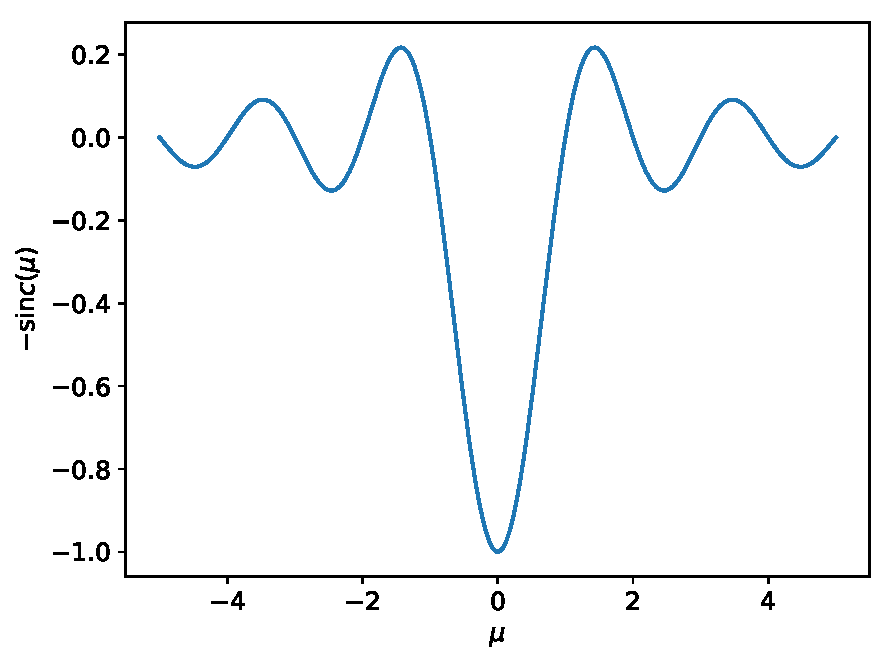
\includegraphics[height=5.7cm]{graphics/var-opt-intu/variational-optimization-function-sinc.pdf}
        \caption{}
        \label{fig: Theory: var-opt-intu-sinc-function}
    \end{subfigure}
    \hfill
    \begin{subfigure}[b]{0.49\textwidth}
        \centering
        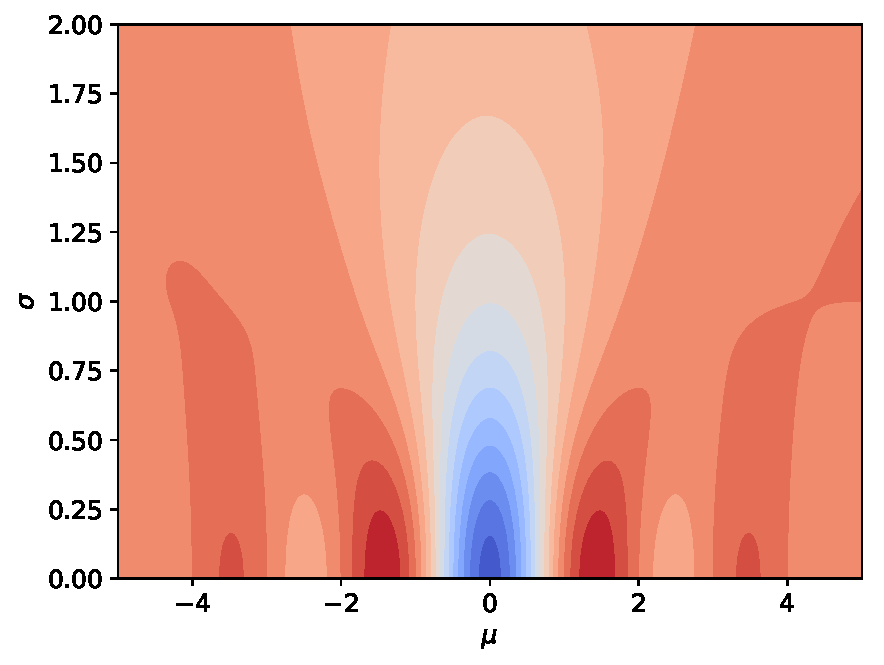
\includegraphics[height=5.7cm]{graphics/var-opt-intu/variational-optimization-contour-sinc.pdf}
        \caption{}
        \label{fig: Theory: var-opt-intu-sinc-contour}
    \end{subfigure}
    \caption{\subref{fig: Theory: var-opt-intu-sinc-function} The negative $\sinc$ function. \subref{fig: Theory: var-opt-intu-sinc-contour} The contours of the Gaussian \gls{VO} objective for the $\sinc$ function for different values of $\mu$ and $\sigma$. Here, the \gls{VO} objective is a two-dimensional upper bounding version of the $\sinc$ function. It tends to a constant for $\sigma\rightarrow\infty$ and the $\sinc$ function for $\sigma\rightarrow0$. The \gls{VO} objective is slightly asymmetrical due to being computed by sampling. Red denotes high values, blue denotes low values and the darker the colour, the higher the absolute value. Actual values are omitted for simplicity. Figures inspired by \cite{Huszar2017}.}
    \label{fig: Theory: var-opt-intu-sinc}
\end{figure}
%
%
The Gaussian \gls{VO} objective function corresponding to the $\sinc$ is visualized in \autoref{fig: Theory: var-opt-intu-sinc-contour} for different values of the search distribution variables $\mu$ and $\sigma^2$. Note especially that optimization is now over the parameters of the search distribution. The global minimum is at $\mu=0$ for any value of $\sigma$. The new objective still has the exact form of the original for $\sigma=0$ and as such still has challenging local minima. However, in this specific case, minimizing the \gls{VO} objective with a fixed value of $\sigma$ of about 1 or larger would uniformly result in approximate\footnote{The convergence will only be to an approximation of the minimum when $\sigma$ is held fixed. This is discussed further in \autoref{sec: Natural Gradient}} convergence on the global minimum regardless of initial point.
Additionally, notice that around the global minimum, $\sinc$ is convex which is also true for the \gls{VO} objective. In fact, for any expectation affine search distribution, which includes Gaussians, if the original objective function is convex then so is the the variational upper bound \cite{Staines2012}.

A quantized version of the $\sinc$ function is seen in \autoref{fig: Theory: var-opt-intu-sinc-quantized-function}. Although this function is non-differentiable, the \gls{VO} bound is still differentiable for any non-zero variance as can be seen in \autoref{fig: Theory: var-opt-intu-sinc-quantized-contour}. As the search distribution variance approaches zero, the \gls{VO} objective tends towards the original objective and non-differentiability. Letting $\sigma\rightarrow\infty$ results in the \gls{VO} objective approaching a constant yielding zero gradient everywhere.
\begin{figure}[tbp!]
    \begin{subfigure}[b]{0.49\textwidth}
        \centering
        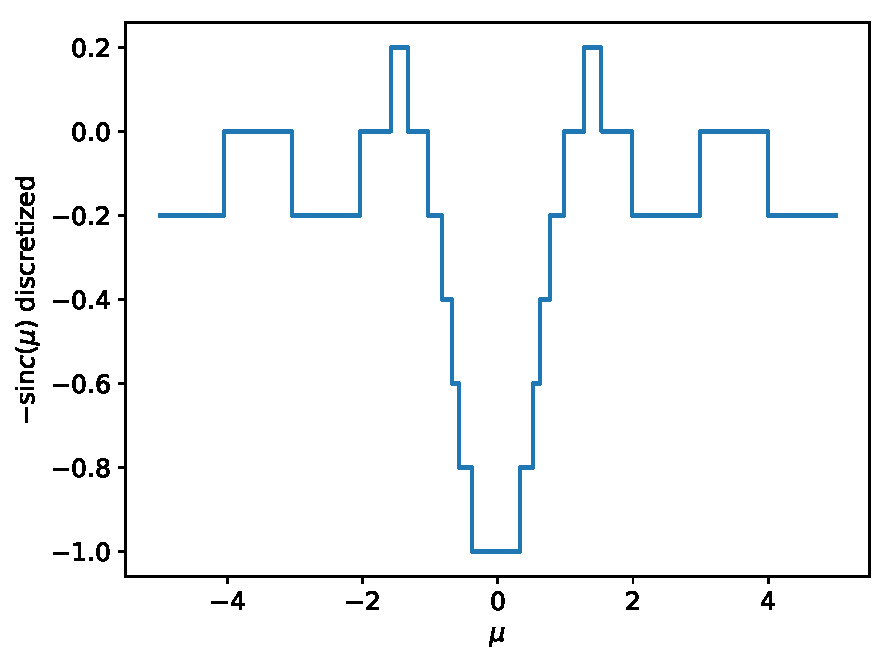
\includegraphics[height=5.7cm]{graphics/var-opt-intu/variational-optimization-function-sinc_quantized.pdf}
        \caption{}
        \label{fig: Theory: var-opt-intu-sinc-quantized-function}
    \end{subfigure}
    \hfill
    \begin{subfigure}[b]{0.49\textwidth}
        \centering
        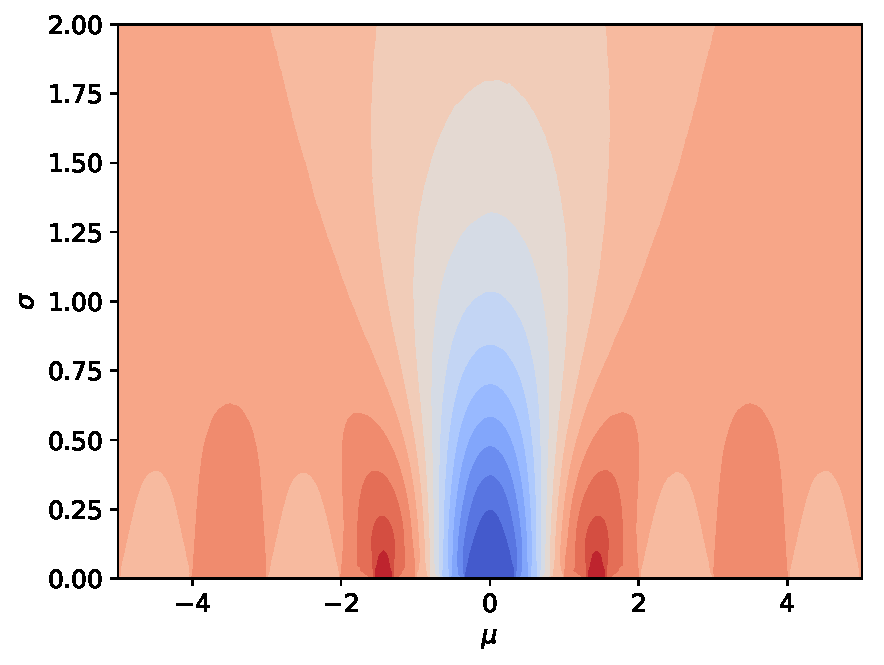
\includegraphics[height=5.7cm]{graphics/var-opt-intu/variational-optimization-contour-sinc_quantized.pdf}
        \caption{}
        \label{fig: Theory: var-opt-intu-sinc-quantized-contour}
    \end{subfigure}
    \caption{\subref{fig: Theory: var-opt-intu-sinc-quantized-function} A quantized version of the $\sinc$ function shown in \autoref{fig: Theory: var-opt-intu-sinc-function}. \subref{fig: Theory: var-opt-intu-sinc-quantized-contour} The contours of the corresponding Gaussian \gls{VO} objective for different values of $\mu$ and $\sigma$. The \gls{VO} objective is a smoothed version of the original nondifferentiable objective tending towards a constant for $\sigma\rightarrow\infty$ and non-differentiability for $\sigma\rightarrow0$. Figures inspired by \cite{Huszar2017}.}
    \label{fig: Theory: var-opt-intu-sinc-quantized}
\end{figure}


A final point should be made about the smoothing of the original objective function done by \gls{VO}. \autoref{fig: Theory: var-opt-intu-narrow-vs-wide-function} shows a function that has a wide local minimum and a narrow global minimum. As seen in \autoref{fig: Theory: var-opt-intu-narrow-vs-wide-contour}, the \gls{VO} objective has a clear preference toward the wide local minimum. The reason for this preference is that the expectation is computed based on a specific value of the variance. The larger the variance, the wider is the range of values on which the function is evaluated and the expectation computed. For large values of $\sigma$, narrow minima are simply averaged out due to the high function values for most sampled points. Thus, Gaussian \gls{VO} has a bias towards minima with low curvature compared to minima with high curvature. This bias is similarly present for other search distributions. 
In relation to this, it is interesting to note that the local structure of the minima of \gls{NN} loss surfaces has been shown to have strong connections to the ability of the resulting network to generalize well. Flatter minima have been claimed to yield better generalization than sharp although the way to define flatness in high dimensional geometries remains somewhat intangible \cite{Garipov2018}.
%
%
\begin{figure}[tbp!]
    \begin{subfigure}[b]{0.49\textwidth}
        \centering
        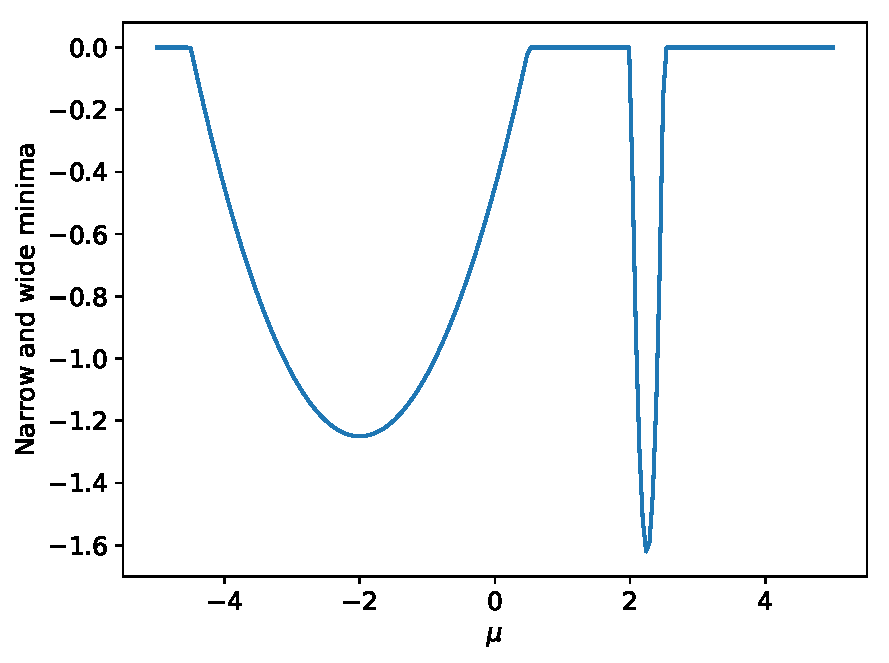
\includegraphics[height=5.7cm]{graphics/var-opt-intu/variational-optimization-function-narrow_vs_wide.pdf}
        \caption{}
        \label{fig: Theory: var-opt-intu-narrow-vs-wide-function}
    \end{subfigure}
    \hfill
    \begin{subfigure}[b]{0.49\textwidth}
        \centering
        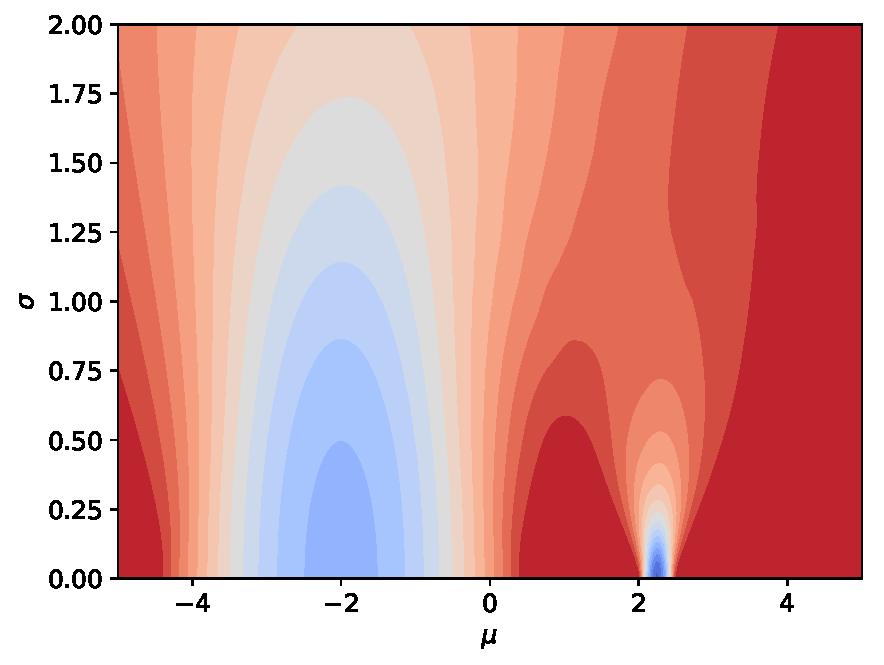
\includegraphics[height=5.7cm]{graphics/var-opt-intu/variational-optimization-contour-narrow_vs_wide.pdf}
        \caption{}
        \label{fig: Theory: var-opt-intu-narrow-vs-wide-contour}
    \end{subfigure}
    \caption{\subref{fig: Theory: var-opt-intu-narrow-vs-wide-function} A function with a low curvature local minimum and a high curvature global minimum. \subref{fig: Theory: var-opt-intu-narrow-vs-wide-contour} The contours of the corresponding Gaussian \gls{VO} objective. The Gaussian \gls{VO} objective has a different global minimum than the original function for almost all values of $\sigma>0$. This illustrates the tendency of \gls{VO} to prefer low curvature minima over high curvature minima if situated near each other. Figures inspired by \cite{Huszar2017}.}
    \label{fig: Theory: var-opt-intu-narrow-vs-wide}
\end{figure}
%
%
\iffalse
\begin{equation}
    \nabla_{\thetab} U({\thetab}) = \text{E}\bra{f(\x)\nabla_{\thetab} \log p(\x|{\thetab})}_{p(\x|{\thetab})}\nonumber\\
\end{equation}


\begin{equation}
    \mathcal{N}(x|\mu,\sigma^2) = \mathcal{N}(\epsilon+\mu|\mu,\sigma^2) = \frac{1}{\sqrt{2\pi\sigma^2}}\exp\left(-\frac{1}{\sigma^2}\epsilon^2\right) = \mathcal{N}(\epsilon|0,\sigma^2)
\end{equation}


Now
\begin{equation}
    \nabla_{\thetab} \log p(x|{\thetab}) = \bmat{\frac{1}{\sigma^2}(x-\mu) \\ -\frac{1}{2\sigma^2} + \frac{1}{4\sigma^4}(x-\mu)^2}
\end{equation}
and
\begin{equation}
    \nabla_{\thetab} U({\thetab}) = \bmat{\pderiv{}{\mu} U(\mu,\sigma^2) \\ \pderiv{}{\sigma^2} U(\mu,\sigma^2)}
\end{equation}

Inserting this in \eqref{eq: Theory: Variational optimization gradient estimator general search distribution} and \eqref{eq: Theory: Variational optimization gradient estimator sampling general search distribution} yields a gradient estimator for optimization of general univariate objective functions
\begin{equation}
    \nabla_{\thetab} U({\thetab}) = \text{E}_{p(\x|{\thetab})}\bra{f(\x)\nabla_{\thetab} \log p(\x|{\thetab})} = \bmat{\pderiv{}{\mu} U(\mu,\sigma^2) \\ \pderiv{}{\sigma^2} U(\mu,\sigma^2)} = \bmat{ \text{E}\left[f(x)\pderiv{}{\mu}\log\mathcal{N}(x|\mu,\sigma^2)\right] \\ \text{E}\left[f(x)\pderiv{}{\sigma^2}\log\mathcal{N}(x|\mu,\sigma^2)\right]}
    %U(\mu,\sigma^2)}\\
    %\nabla_{\thetab}\text{E}_{p(\x|{\thetab})}\bra{f(\x)}\nonumber\\
%&= \text{E}_{p(\x|{\thetab})}\bra{f(\x)\nabla_{\thetab} \log p(\x|{\thetab})}\nonumber\\
%&\approx \frac{1}{N}\sum_{n=1}^N f(\x_n)\nabla_{\thetab} \log p(\x_n|{\thetab}))
\end{equation}
\fi




%\subsubsection{The non-general equality of the Taylor series gradients and the variational upper bound gradients}
\subsubsection{The difference between the VO and Taylor series gradients}
Following the observation that the Taylor gradient and the \gls{VO} gradient are equivalent for a Gaussian perturbation/search distribution, it should be noted the two approaches are not in general equivalent for different choices of search distributions. As an example, take the Laplace distribution,
\begin{equation}
    p(x|\mu,b) = \frac{1}{2b}\exp\pa{-\frac{\size{x-\mu}}{b}} = \frac{1}{\sqrt{2}\sigma}\exp\pa{-\frac{\sqrt{2}}{\sigma}\size{x-\mu}}
\end{equation}
with mean $\mu$ and variance $\sigma=\sqrt{2}b$. The first three moments of the Laplace distribution are needed for the Taylor gradient estimator and can be computed as follows. Let $\epsilon = x-\mu$ from which it follows that $d\epsilon = dx$. The first moment is
\begin{align}
    \text{E}\bra{x}
    &= \text{E}\bra{\epsilon}+\mu\nonumber\\
    &= \frac{1}{2b}\int_{-\infty}^{\infty} \epsilon \exp\pa{-\frac{\size{\epsilon}}{b}}\;\text{d}\epsilon + \mu\nonumber\\
    &= \frac{1}{2b}\pa{\int_{-\infty}^{0} \epsilon \exp\pa{\frac{\epsilon}{b}}\;\text{d}\epsilon + \int_{0}^{\infty} \epsilon \exp\pa{-\frac{\epsilon}{b}}\;\text{d}\epsilon} + \mu\nonumber\\
    &= \mu \ .
\end{align}
Using that $\text{E}\bra{\epsilon}=0$ as computed above, the second moment becomes
\begin{align}
    \text{E}\bra{x^2}
    &= \text{E}\bra{(\epsilon+\mu)^2}\nonumber\\
    %&= \text{E}\bra{\epsilon^2} + 2\mu\text{E}\bra{\epsilon} + \mu^2\nonumber\\
    &= \text{E}\bra{\epsilon^2} + \mu^2\nonumber\\
    &= \frac{1}{2b}\int_{-\infty}^{\infty} \epsilon^2 \exp\pa{-\frac{\size{\epsilon}}{b}}\;\text{d}\epsilon + \mu^2\nonumber\\
    &= \frac{1}{2b}\pa{\int_{-\infty}^{0} \epsilon^2 \exp\pa{\frac{\epsilon}{b}}\;\text{d}\epsilon + \int_{0}^{\infty} \epsilon^2 \exp\pa{-\frac{\epsilon}{b}}\;\text{d}\epsilon} + \mu^2\nonumber\\
    %&= \frac{1}{2b}\pa{\int_{0}^{\infty} \epsilon^2 \exp\pa{-\frac{\epsilon}{b}}\;\text{d}\epsilon^2 + \int_{0}^{\infty} \epsilon^2 \exp\pa{-\frac{\epsilon}{b}}\;\text{d}\epsilon} + \mu^2\nonumber\\
    &= \frac{1}{b}\int_{0}^{\infty} \epsilon^2 \exp\pa{-\frac{\epsilon}{b}}\;\text{d}\epsilon + \mu^2,\nonumber\\
\shortintertext{and substituting $v=\frac{\epsilon}{b},\;\text{d}v = \text{d}\epsilon$,}
    \text{E}\bra{x^2} &= b^2\int_{0}^{\infty} v^2 \exp\pa{-v}\;\text{d}\epsilon + \mu^2\nonumber\\
    &= 2b^2 + \mu \ .
\end{align}
% \begin{align}
%     \text{E}\bra{x^2}
%     &= \text{E}\bra{(\epsilon+\mu)^2}\nonumber\\
%     &= \text{E}\bra{\epsilon^2} + 2\mu\text{E}\bra{\epsilon} + \mu^2\nonumber\\
%     &= \text{E}\bra{\epsilon^2} + \mu^2\nonumber\\
%     &= \frac{1}{2b}\int_{-\infty}^{\infty} \epsilon^2 \exp\pa{-\frac{\size{\epsilon}}{b}}\;\text{d}\epsilon + \mu^2\nonumber\\
%     &= \frac{1}{2b}\pa{\int_{-\infty}^{0} \epsilon^2 \exp\pa{\frac{\epsilon}{b}}\;\text{d}\epsilon + \int_{0}^{\infty} \epsilon^2 \exp\pa{-\frac{\epsilon}{b}}\;\text{d}\epsilon} + \mu^2\nonumber\\
%     &= \frac{1}{2b}\pa{\int_{0}^{\infty} \epsilon^2 \exp\pa{-\frac{\epsilon}{b}}\;\text{d}\epsilon^2 + \int_{0}^{\infty} \epsilon^2 \exp\pa{-\frac{\epsilon}{b}}\;\text{d}\epsilon} + \mu^2\nonumber\\
%     &= \frac{1}{b}\int_{0}^{\infty} \epsilon^2 \exp\pa{-\frac{\epsilon}{b}}\;\text{d}\epsilon + \mu^2\nonumber\\
%     &= b^2\int_{0}^{\infty} v^2 \exp\pa{-v}\;\text{d}\epsilon + \mu^2,\qquad\qquad \text{substitution: } v=\frac{\epsilon}{b},\;dv = d\epsilon \nonumber\\
%     &= 2b^2 + \mu.
% \end{align}
Finally, the third moment is
\begin{align}
    \text{E}\bra{x^3}
    &= \text{E}\bra{(\epsilon+\mu)^3}\nonumber\\
    &= \text{E}\bra{\epsilon^3} + 3\mu\text{E}\bra{\epsilon^2} + 3\mu^2\text{E}\bra{\epsilon} - \mu^3\nonumber\\
    %&= \text{E}\bra{\epsilon^3} + 6b^2\mu + \mu^3\nonumber\\
    &= \frac{1}{2b}\int_{-\infty}^{\infty} \epsilon^3 \exp\pa{-\frac{\size{\epsilon}}{b}}\;\text{d}\epsilon + 6b^2\mu + \mu^3\nonumber\\
    &= \frac{1}{2b}\pa{\int_{-\infty}^{0} \epsilon^3 \exp\pa{\frac{\epsilon}{b}}\;\text{d}\epsilon + \int_{0}^{\infty} \epsilon^3 \exp\pa{-\frac{\epsilon}{b}}\;\text{d}\epsilon} + 6\mu(b^2 + \mu^2)\nonumber\\
    %&= \frac{1}{2b}\pa{-\int_{0}^{\infty} \epsilon^3 \exp\pa{-\frac{\epsilon}{b}}\;\text{d}\epsilon + \int_{0}^{\infty} \epsilon^3 \exp\pa{-\frac{\epsilon}{b}}\;\text{d}\epsilon} + 6b^2\mu + \mu^3\nonumber\\
    &= 6\mu(b^2 + \mu^2) \ .
\end{align}

For a Laplace distributed perturbation $\epsilon\sim p(\epsilon|0,b)$, it follows that the first moment is zero, the second moment is $2b^2=\sigma^2$ and the third moment is also zero, similarly to the Gaussian.
The Taylor series gradient then becomes identical to that using a zero mean Gaussian perturbation\footnote{The derivation of the Gaussian perturbation Taylor gradient in \autoref{sec: Theory: stochastic gradient by Taylor expoansion} only exploits that the odd moments of the Gaussian search distribution are zero. As such, that derivation holds equally well for the Laplace distribution which also has odd moments equal to zero.},
\begin{equation}
    f'(x) \approx \frac{1}{2Nb^2}\sum_{n=1}^N f(x+\epsilon_n)\epsilon_n = \frac{1}{N\sigma^2}\sum_{n=1}^N f(x+\epsilon_n)\epsilon_n \ ,\label{eq: Theory: Variational optimization Taylor VS VO for Laplace (Taylor)}
\end{equation}
only now with a Laplacian perturbation.

The \gls{VO} gradient however differs from the Taylor gradient. The log of the Laplace \gls{PDF} is
\begin{equation}
    \log p(x|\mu,b) = -\log(2b) - \frac{1}{b}\size{x-\mu}
\end{equation}
such that the search distribution gradient is
\begin{equation}
    \begin{aligned}
        \frac{\partial}{\partial\mu} \log p(x|\mu,b) &= \frac{1}{b}\text{sgn}(x-\mu)\\
        \frac{\partial}{\partial b} \log p(x|\mu,b) &= -\frac{1}{b}+\frac{1}{b^2}\size{x-\mu}\\
    \end{aligned}
\end{equation}
where $\text{sgn}(\cdot)$ is the sign function. It then follows from \eqref{eq: Theory: Variational optimization gradient estimator general search distribution} that $f'(x) = \frac{1}{b}\text{E}\bra{f(x)\,\text{sgn}(\epsilon)}$ and by Monte Carlo sampling,
\begin{equation}
    f'(x) \approx \frac{1}{Nb}\sum_{i=1}^N f(x+\epsilon_n)\,\text{sgn}(\epsilon_n) = \frac{\sqrt{2}}{N\sigma}\sum_{i=1}^N f(x+\epsilon_n)\,\text{sgn}(\epsilon_n)\label{eq: Theory: Variational optimization Taylor VS VO for Laplace (VO)}
\end{equation}
with $\epsilon\sim p(x|0,b)$.

Clearly, the \gls{VO} gradient in \eqref{eq: Theory: Variational optimization Taylor VS VO for Laplace (VO)} differs from the Taylor gradient in \eqref{eq: Theory: Variational optimization Taylor VS VO for Laplace (Taylor)} by using the sign of the perturbation rather than the perturbation itself (and a factor of $\sqrt{2}$). 
The Taylor gradient is slightly biased, which follows from the derivation in \autoref{sec: Theory: stochastic gradient by Taylor expoansion}.
The Taylor gradient also implicitly assumes that the objective function is differentiable although practically, this does not have to be the case when using a Monte Carlo estimator as long as the estimator converges. The \gls{VO} gradient on the other hand is an unbiased estimate of the gradient of the differentiable upper bound to a possibly non-differentiable objective function defined by \eqref{eq: Theory: Variational optimization variational upper bound}. The choice is then between a biased estimate of the gradient of the objective or an unbiased estimate of an (arbitrarily tight) upper bound of the objective.

It can be noted that for distributions with undefined moments, e.g. the heavy tailed Cauchy distribution, the Taylor series gradient estimator does not exist while the \gls{VO} search gradient does. This difference is due to the Taylor series derivation relying on the existence of the moments of the chosen distribution as well as the exploitation of some of these moments being zero, e.g. the odd moments of the Gaussian.


\subsubsection{Multivariate Gaussian search distribution}\label{sec: Theory: Variational optimization: Multivariate Gaussian search distribution}
In the most general case, the Gaussian search distribution is multivariate and parameterizes the full covariance matrix. Then $p(\x|\thetab)=\mathcal{N}(\x|\mub,\Sigmab)$ is given by
\begin{equation}\label{eq: Theory: Variational optimization multivariate Gaussian PDF}
    \mathcal{N}(\x|\mub,\Sigmab) = \frac{1}{(2\pi)^{\sfrac{d}{2}}\size{\Sigmab}^{\sfrac{1}{2}}}\exp\pa{-\frac{1}{2}(\x-\mub)\transpose\Sigmab^{-1}(\x-\mub)}
\end{equation}
with $\thetab = \{\mub, \Sigmab\}$. It follows that
\begin{equation}\label{eq: Theory: Variational optimization multivariate Gaussian log PDF}
    \log\mathcal{N}(\x|\mub,\Sigmab) = -\frac{d}{2}\log(2\pi) - \frac{1}{2}\log\size{\Sigmab} -  \frac{1}{2}(\x-\mub)\transpose\Sigmab^{-1}(\x-\mub) \ .
\end{equation}
For a matrix $\A$ and column vectors $\a$ and $\b$, the following relations exist for the gradients w.r.t. $\A$ of the determinant of $\A$ and the quadratic form $\a\transpose\A\b$ \cite[(49) and (61)]{Petersen2012}.
\begin{align*}
    \nabla_\A \size{\A} &= \size{\A}\pa{\A^{-1}}\transpose\\
    \nabla_\A \a\transpose\A\b &= -\A\a\b\transpose\A\transpose \ .
\end{align*}
Using these for the computing the gradient w.r.t. $\Sigmab$, the gradients of the logarithm of the Gaussian are
\begin{align}
    \nabla_\mub\log\mathcal{N}(\x|\mub,\Sigmab)
    &= \Sigmab^{-1}(\x-\mub)\\
    \nabla_\Sigmab\log\mathcal{N}(\x|\mub,\Sigmab)
    &= -\frac{1}{2}\Sigmab^{-1} + \frac{1}{2}\Sigmab^{-1}(\x-\mub)(\x-\mub)\transpose\Sigmab^{-1} \ .
\end{align}
As for the univariate case, a change of variables can be made such that $\x=\mub+\L\epsilonb$ where $\L$ is the Cholesky factor of the covariance matrix, $\Sigmab=\L\L\transpose$ and $\epsilonb\sim\mathcal{N}(\0,\I)$. The Cholesky factor is guaranteed to exist since the covariance matrix is symmetric and positive-definite. Then \eqref{eq: Theory: Variational optimization variational upper bound} becomes
\begin{equation}
    U(\mub,\L) = \text{E}\bra{f(\x)}_{\mathcal{N}(\x|{\mub,\Sigmab})}  = \text{E}\bra{f(\mub + \L\epsilonb)}_{\mathcal{N}(\epsilonb|{\0,\I})}.
\end{equation}
Applying the Cholesky factorization and this change of variables, the gradients can be simplified as follows.
\begin{align}
    \nabla_\mub\log\mathcal{N}(\x|\mub,\Sigmab)
    %&= \Sigmab^{-1}(\x-\mub)\\
    &= (\L\L\transpose)^{-1}\L\epsilonb\nonumber\\
    &= (\L\transpose)^{-1}\L^{-1}\L\epsilonb\nonumber\\
    &= (\L^{-1})\transpose\epsilonb
\end{align}
and
\begin{align}
    \nabla_\Sigmab\log\mathcal{N}(\x|\mub,\Sigmab)
    %&= -\frac{1}{2}\Sigmab^{-1} + \frac{1}{2}\Sigmab^{-1}(\x-\mub)(\x-\mub)\transpose\Sigmab^{-1}\\
    &= -\frac{1}{2}(\L\L\transpose)^{-1} + \frac{1}{2}(\L\L\transpose)^{-1}\L\epsilonb(\L\epsilonb)\transpose(\L\L\transpose)^{-1}\nonumber\\
    &= -\frac{1}{2}(\L\L\transpose)^{-1} + \frac{1}{2}(\L\transpose)^{-1}\L^{-1}\L\epsilonb\epsilonb\transpose\L\transpose(\L\transpose)^{-1}\L^{-1}\nonumber\\
    &= -\frac{1}{2}(\L\L\transpose)^{-1} + \frac{1}{2}(\L\transpose)^{-1}\epsilonb\epsilonb\transpose\L^{-1} \ .
\end{align}
With these gradients, the \gls{VO} gradient estimator becomes
\begin{equation}\label{eq: Theory: Variational optimization multivariate gaussian gradient estimators}
    \begin{aligned}
        \nabla_\mub U(\mub,\L) &= (\L^{-1})\transpose\text{E}\bra{f(\mub+\L\epsilonb)\epsilonb} \approx \frac{(\L^{-1})\transpose}{N}\sum_{n=1}^N f(\mub+\L\epsilonb_n)\epsilonb_n\\
        \nabla_\Sigmab U(\mub,\L) &= \text{E}\bra{f(\mub+\L\epsilonb)\pa{-\frac{1}{2}(\L\L\transpose)^{-1} + \frac{1}{2}(\L\transpose)^{-1}\epsilonb\epsilonb\transpose\L^{-1}}} \ .
    \end{aligned}
\end{equation}
Using the full covariance matrix will result in the most flexible Gaussian search distribution. However, too much flexibility could be harmful as it runs the risk of overfitting the search distribution \cite{Magdon-Ismail2010}. Additionally, the full covariance matrix can be inhibitingly large to use with its $d(d+1)/2$ parameters.  If optimizing in high dimensional spaces, such as the parameter spaces of \glspl{NN}, it is computationally infeasible as these can have $d$ anywhere from thousands to hundreds of millions. This infeasibility arises, if not as a memory problem, then due to the computational time complexity of matrix inversion being cubic as a function of matrix dimension, $d$.
Another concern for full covariance matrices is sample efficiency. Due to the large number of parameters of the covariance matrix, obtaining a good estimate of its gradient may require many function evaluations, which can be costly. Therefore, the optimization algorithm may not have time enough to adapt the search distribution well \cite{Schaul2011}. Finally, sampling from a Gaussian distribution with $d$ very large can be slow due to the large matrix vector product, $\L\epsilonb$.
Thus, for high dimensional search spaces, alternatives to the full covariance are needed.

%\todo[inline]{Update the section on the multivariate Gaussian search distribution with gradients wrt. $\L$ rather than $\Sigma$}


\subsubsection{Isotropic Gaussian search distribution}\label{sec: Theory: Variational optimization: Isotropic Gaussian search distribution}
The most radical alternative to the full covariance is to use an isotropic parameterization of the covariance matrix. An isotropic parameterization is given by a single variance repeated in every dimension with no covariances, $\Sigmab = \sigma^2\I$. In this case, $p(\x|{\thetab}) = \mathcal{N}(\x|\mub,\sigma^2\I)$ is called an isotropic Gaussian distribution and can be written as
\begin{align}
    \mathcal{N}(\x|\mub,\sigma^2\I)
    &= \frac{1}{(2\pi)^{\sfrac{d}{2}}\size{\sigma^2\I}^{\sfrac{1}{2}}}\exp\pa{-\frac{1}{2}(\x-\mub)\transpose(\sigma^2\I)^{-1}(\x-\mub)}\nonumber\\
    &= \frac{1}{(2\pi)^{\sfrac{d}{2}}\sigma^d}\exp\pa{-\frac{1}{2\sigma^2}(\x-\mub)\transpose(\x-\mub)}
\end{align}
since
\begin{equation}
    \size{\sigma^2\I}^{\sfrac{1}{2}} = \sqrt{\prod_{i=1}^d \sigma^2} 
    %= \left[\prod_{i=1}^d \sigma^2\right]^{\sfrac{1}{2}} 
    = \sqrt{\sigma^{2d}} = \sigma^d \ .
\end{equation}
The log-\gls{PDF} is
\begin{equation}\label{eq: Theory: Variational optimization multivariate isotropic gaussian log pdf}
    \log\mathcal{N}(\x|\mub,\sigma^2\I) = -\frac{d}{2}\log(2\pi) - \frac{d}{2}\log(\sigma^2) - \frac{1}{2\sigma^2}(\x-\mub)\transpose(\x-\mub) \ .
\end{equation}
Again, let $\x=\mub+\sigma^2\epsilonb$ so \eqref{eq: Theory: Variational optimization variational upper bound} becomes
\begin{equation}
    U(\mub,\sigma^2) = \text{E}\bra{f(\x)}_{\mathcal{N}(\x|{\mub,\sigma^2\I})}  = \text{E}\bra{f(\mub + \sigma\epsilonb)}_{\mathcal{N}(\epsilonb|{\0,\I})} \ .
\end{equation}
It follows that
\begin{equation}\label{eq: Theory: Variational optimization multivariate isotropic gaussian search gradients}
    \begin{aligned}
        \nabla_\mub \log\mathcal{N}(\x|\mub,\sigma^2\I) &= \frac{1}{\sigma^2}(\x-\mub) = \frac{1}{\sigma}\epsilonb\\
        \nabla_{\sigma^2} \log\mathcal{N}(\x|\mub,\sigma^2\I) &= -\frac{d}{2\sigma^2} + \frac{1}{2\sigma^4}(\x-\mub)\transpose(\x-\mub) = \frac{1}{2\sigma^2}\left(\epsilonb\transpose\epsilonb - d\right) \ .
    \end{aligned}
\end{equation}
By \eqref{eq: Theory: Variational optimization gradient estimator general search distribution}, the gradient of the \gls{VO} objective with an isotropic Gaussian search distribution is
\begin{equation}
    \begin{aligned}
        \nabla_\mub U(\mub,\sigma^2) &= \frac{1}{\sigma}\text{E}\bra{f(\mub + \sigma\epsilonb)\epsilonb} \approx \frac{1}{N\sigma}\sum_{n=1}^N f(\mub+\sigma\epsilonb_n)\epsilonb_n\\
        \nabla_{\sigmab^2} U(\mub,\sigma^2) &= \frac{1}{2\sigma^2}\text{E}\bra{f(\mub + \sigma\epsilonb)\left(\epsilonb\transpose\epsilonb-d\right)} \approx \frac{1}{2N\sigma^2}\sum_{n=1}^N f(\mub + \sigma\epsilonb_n)\left(\epsilonb_n\transpose\epsilonb_n-d\right) \ .
    \end{aligned}\label{eq: Theory: Variational optimization multivariate isotropic gaussian gradient estimators}
\end{equation}
This is evidently a simple generalization of univariate case in \eqref{eq: Theory: Variational optimization univariate gaussian gradient estimators} to the $d$-dimensional case while keeping the variance scalar. Compared to the general Gaussian search distribution, the isotropic Gaussian has only a single variance parameter to be optimized. As a consequence, it is much less memory intensive and sampling can be done in $O(d)$ time. However, the distribution captures no covariance between the dimensions being searched and the smoothing of the objective is the same in all dimensions. 






\subsubsection{Separable Gaussian search distribution}\label{sec: Theory: Variational optimization: Separable Gaussian search distribution}
A more flexible version of the Gaussian search distribution compared to the isotropic special case is the separable Gaussian. Similarly to the isotropic Gaussian, the separable Gaussian captures no covariance information between the dimensions. Instead, it parameterizes the covariance matrix by $d$ individual variance parameters along its diagonal. The \gls{PDF} is defined as for the multivariate Gaussian in \eqref{eq: Theory: Variational optimization multivariate Gaussian PDF} but with $\Sigmab=\text{diag}\pa{\sigma_1^2, \sigma_2^2, \dots, \sigma_d^2}$. Let
\begin{equation}
    \sigmab^2 = \bmat{\sigma_1^2 & \sigma_2^2 & \cdots & \sigma_d^2}^\text{T}
\end{equation}
be the parameter vector holding the variances with squaring applied elementwise. Then
\begin{equation}\label{eq: Theory: Variational optimization separable Gaussian Sigma matrix simplification}
    \Sigmab = \text{diag}\pa{\sigmab^2}% = \pa{\sigmab^2\e\transpose}\odot\I
\end{equation}
where $\e=\bmat{1&1&\cdots&1}\transpose$ and the $\odot$ operator denotes elementwise multiplication. Inserting this expression for $\Sigmab$ into the log-\gls{PDF} of the Gaussian in \eqref{eq: Theory: Variational optimization multivariate Gaussian log PDF} gives the logarithm of the separable Gaussian \gls{PDF} which can be simplified by noting,
% \begin{equation}\label{eq: Theory: Variational optimization: Separable Gaussian log pdf (complex)}
%     \log\mathcal{N}\pa{\x|\mub, (\sigmab^2\e\transpose)\odot\I} = - \frac{1}{2}\log\pa{(2\pi)^\frac{d}{2}\size{(\sigmab^2\e\transpose)\odot\I}} - \frac{1}{2}(\x-\mub)\transpose\pa{(\sigmab^2\e\transpose)\odot\I}^{-1}(\x-\mub).
    %\begin{split}
        %\log\mathcal{N}\pa{\x|\mub, (\sigmab^2\e\transpose)\odot\I} &= -\frac{d}{2}\log(2\pi) - \frac{1}{2}\log\size{(\sigmab^2\e\transpose)\odot\I} - \frac{1}{2}(\x-\mub)\transpose\pa{(\sigmab^2\e\transpose)\odot\I}^{-1}(\x-\mub).
    %\end{split}
% \end{equation}
% \todo[inline]{This equation spans multiple lines, maybe it can be put on a single line?}
% Now, it can be seen that
\begin{align}
    \log\size{\Sigmab}
    &= \log\size{\text{diag}\pa{\sigmab^2}}\nonumber\\
    &= \log\prod_{i=1}^d \sigma_i^2\nonumber\\
    &= \sum_{i=1}^d \log\sigma_i^2\nonumber\\
    &= \e\transpose\log\pa{\sigmab^2} \ .\label{eq: Theory: Variational optimization: Separable Gaussian log of determinant vectorized form}
\end{align}
Likewise for the quadratic form,
\begin{align} %(\x-\mub)\transpose\Sigmab^{-1}(\x-\mub)
    (\x-\mub)\transpose\Sigmab^{-1}(\x-\mub)
    &= (\x-\mub)\transpose\text{diag}\pa{\sigmab^{-2}}(\x-\mub)\label{eq: Theory: Variational optimization: Separable Gaussian quadratic form diagonal matrix version}\\
    &= \sum_{i=1}^d \frac{(x_i-\mu_i)^2}{\sigma_i^2}\nonumber\\
    &= \pa{\sigmab^{-2}}\transpose(\x-\mub)^2 \ .\label{eq: Theory: Variational optimization: Separable Gaussian quadratic form squared vectors version}
\end{align}
Here, the inverse squaring of $\sigmab$ is applied elementwise, $\sigmab^{-2}=\bmat{\sigma_1^{-2} & \sigma_2^{-2} & \dots & \sigma_d^{-2}}^\text{T}$. From \eqref{eq: Theory: Variational optimization: Separable Gaussian log of determinant vectorized form} and \eqref{eq: Theory: Variational optimization: Separable Gaussian quadratic form squared vectors version} it follows that
\begin{equation}\label{eq: Theory: Variational optimization: Separable Gaussian log pdf (simplified through vectorization)}
    \log\mathcal{N}\pa{\x|\mub, (\sigmab^2\e\transpose)\odot\I} = -\frac{d}{2}\log(2\pi) - \frac{1}{2}\e\transpose\log\pa{\sigmab^2} - \frac{1}{2}\pa{\sigmab^{-2}}\transpose(\x-\mub)^2 \ .
\end{equation}
As before, reparameterize $\x = \mub + \sigmab\odot\epsilonb$ so
\begin{equation}
    U(\mub,\sigma^2) = \text{E}\bra{f(\x)}_{\mathcal{N}(\x|{\mub,(\sigmab^2\e\transpose)\odot\I})}  = \text{E}\bra{f(\mub + \sigmab\odot\epsilonb)}_{\mathcal{N}(\epsilonb|\0,\I)} \ .
\end{equation}
Using the quadratic form in \eqref{eq: Theory: Variational optimization: Separable Gaussian quadratic form diagonal matrix version}, the gradient w.r.t. $\mub$ is
\begin{align}\label{eq: Theory: Variational optimization multivariate isotropic gaussian search gradients (mub)}
    \nabla_\mub \log\mathcal{N}(\x|\mub,(\sigmab^2\e\transpose)\odot\I)
    &= \frac{1}{2}\nabla_\mub \pa{\sigmab^{-2}}\transpose(\x-\mub)^2 \nonumber\\
    %&= \pa{(\sigmab^{-2}\e\transpose)\odot\I}(\x-\mub) \nonumber\\
    &= \sigmab^{-2} \odot (\x-\mub) \nonumber\\
    &= \sigmab^{-1} \odot \epsilonb \ .
\end{align}
Using the quadratic form \eqref{eq: Theory: Variational optimization: Separable Gaussian quadratic form squared vectors version}, the gradient w.r.t. $\sigmab^2$ is
\begin{align}\label{eq: Theory: Variational optimization multivariate isotropic gaussian search gradients (sigmab^2)}
    \nabla_{\sigmab^2} \log\mathcal{N}(\x|\mub,(\sigmab^2\e\transpose)\odot\I)
    &= - \frac{1}{2}\nabla_{\sigmab^2}\e\transpose\log\sigmab^2 - \frac{1}{2}\nabla_{\sigmab^2}\pa{\sigmab^{-2}}^\text{T}(\x-\mub)^2 \nonumber\\
    &= - \frac{1}{2}\sigmab^{-2}+ \frac{1}{2}\text{diag}\pa{\sigmab^{-4}}(\x-\mub)^2 \nonumber\\
    %&= - \frac{1}{2}\bmat{\sigma_1^{-2} \\ \vdots \\ \sigma_d^{-2}} + \frac{1}{2}\bmat{\sigma_1^{-4}(x_1 -\mu_1)^2\\\vdots\\\sigma_d^{-4}(x_d-\mu_d)^2} \nonumber\\
    &= -\frac{1}{2}\sigmab^{-2} + \frac{1}{2} \sigmab^{-4}\odot(\x-\mub)^2\nonumber\\
    &= -\frac{1}{2}\sigmab^{-2} \odot \pa{\epsilonb^2 - 1} \ .
\end{align}
By \eqref{eq: Theory: Variational optimization gradient estimator general search distribution}, the gradient of the \gls{VO} objective becomes
\begin{align}
    \nabla_\mub U(\mub,\sigma^2) &= \sigmab^{-1}\odot\text{E}\bra{f(\mub + \sigmab\odot\epsilonb)\epsilonb} \approx \sigmab^{-1}\odot\frac{1}{N}\sum_{n=1}^N f(\mub+\sigmab\odot\epsilonb_n)\epsilonb_n\label{eq: Theory: Variational optimization separable gaussian gradient estimators}\\
    \nabla_\sigma^2 U(\mub,\sigma^2) &= \frac{1}{2}\sigmab^{-2}\odot\text{E}\bra{f(\mub + \sigmab\odot\epsilonb)\pa{\epsilonb^2 - 1}} \approx \sigmab^{-2}\odot\frac{1}{2N}\sum_{n=1}^N f(\mub + \sigmab\odot\epsilonb_n)\pa{\epsilonb_n^2 - 1} \ .\nonumber
\end{align}
% \begin{equation}
%     \begin{aligned}
%         \nabla_\mub U(\mub,\sigma^2) &= \sigmab^{-1}\odot\text{E}\bra{f(\mub + \sigmab\odot\epsilonb)\epsilonb} \approx \sigmab^{-1}\odot\frac{1}{N}\sum_{n=1}^N f(\mub+\sigmab\odot\epsilonb_n)\epsilonb_n\\
%         \nabla_\sigma^2 U(\mub,\sigma^2) &= \frac{1}{2}\sigmab^{-2}\odot\text{E}\bra{f(\mub + \sigmab\odot\epsilonb)\pa{\epsilonb^2 - 1}} \approx \sigmab^{-2}\odot\frac{1}{2N}\sum_{n=1}^N f(\mub + \sigmab\odot\epsilonb_n)\pa{\epsilonb_n^2 - 1}\\
%     \end{aligned}\label{eq: Theory: Variational optimization separable gaussian gradient estimators}
% \end{equation}

Note that these gradients are in fact the gradients of the univariate Gaussian in each dimension of the separable Gaussian. That this must be the case can also be seen by rewriting the $d$ dimensional separable Gaussian as a product of univariate Gaussians as follows.
\begin{align}
    \mathcal{N}\pa{\x|\mub, \text{diag}(\sigmab^2)}
    &= \frac{1}{(2\pi)^{\sfrac{d}{2}}\size{\text{diag}(\sigmab^2)}^{\sfrac{1}{2}}}\exp\pa{-\frac{1}{2}(\x-\mub)\transpose\text{diag}(\sigmab^2)^{-1}(\x-\mub)}\nonumber\\
    &= \frac{1}{(2\pi)^{\sfrac{d}{2}}\prod_{i=1}^d \sigma_i}\exp\pa{-\frac{1}{2} 
    \bmat{x_1-\mu_1\\\vdots\\x_d-\mu_d}^\text{T}
    \bmat{\sigma_1^{-2} & \cdots & 0\\
          \vdots        & \ddots & \vdots\\
          0             & \cdots & \sigma_d^{-2}}
    \bmat{x_1-\mu_1\\\vdots\\x_d-\mu_d}}\nonumber\\
    &= \frac{1}{\prod_{i=1}^d (2\pi)^{\sfrac{1}{2}}\sigma_i}\exp\pa{-\sum_{i=1}^d\frac{(x_i-\mu_i)^2}{2\sigma_i^2}}\nonumber\\
    &= \frac{1}{\prod_{i=1}^d \sqrt{2\pi}\sigma_i}\prod_{i=1}^d\exp\pa{-\frac{(x_i-\mu_i)^2}{2\sigma_i^2}} \nonumber\\
    &= \prod_{i=1}^d\frac{1}{\sqrt{2\pi}\sigma_i}\exp\pa{-\frac{(x_i-\mu_i)^2}{2\sigma_i^2}}\nonumber\\
    &= \prod_{i=1}^d\mathcal{N}(x_i|\mu_i,\sigma_i^2) \ .
\end{align}
Then
\begin{equation}
    \log\mathcal{N}\pa{\x|\mub, \text{diag}(\sigmab^2)} = \log\prod_{i=1}^d\mathcal{N}(x_i|\mu_i,\sigma_i^2) = \sum_{i=1}^d \log\mathcal{N}(x_i|\mu_i,\sigma_i^2)
\end{equation}
which is simply a sum of univariate Gaussians. Since each dimension is independent from the others, taking the derivative of $\log\mathcal{N}\pa{\x|\mu, \Sigmab}$ w.r.t. $\sigmab$ simply returns the derivative of a univariate Gaussian in each dimension as in \eqref{eq: Theory: Variational optimization separable gaussian gradient estimators}.

Compared to the isotropic Gaussian, the separable Gaussian has $d$ variances rather than one which allows greater flexibility during the search and potentially faster convergence. Compared to the general multivariate Gaussian, the number of parameters is linear in the dimension rather than quadratic. 

Using \gls{VO} with a separable Gaussian search distribution to train an \gls{NN} requires storing the weights as the mean parameter and as many variance parameters as there are weights. This significantly adds to the number of parameters held in memory during training but this is possible for many network models which already store the weights, their gradients and potentially associated momentum buffers.
An alternative approach is to consider only a subset of the trained \gls{NN} weights as independent dimensions. One way to do this is to define each network layer as a dimension and parameterize a unique variance only for every layer. Perturbations are then sampled from the corresponding dimension of the search distribution for each weight of the specific layer. These approaches will be examined in \autoref{chp: Experimental results}.


\subsubsection{Low rank covariance matrix approximation}\label{sec: Variational optimization: Low rank approximation}
Low rank approximations of the covariance matrix allows for a significant reduction of the number of parameters from being quadratic in dimension to being linear in dimension. Such approximations have been applied several places such as for training Gaussian Mixture Models \cite{Magdon-Ismail2010}. However, much of the previous work is concerned with optimization of the low rank approximation by maximum likelihood and the likes of it with the goal of fitting a model \cite{Belabbas2007, Duan2014, Turek2017}. This is somewhat different from the case of variational optimization where the covariance matrix is not fitted per say but rather updated continuously to give the best samples for making progress in some optimization problem. 
This section introduces the truncated SVD approximation which is one way of forming a theoretical background for low rank matrix approximations.

Any general, real valued matrix $\A$ can be decomposed as
\begin{equation}
    \underset{N\times D}{\underbrace{\A}} = \underset{N\times N}{\underbrace{\U}}\;\underset{N\times D}{\underbrace{\S}}\;\underset{D\times D}{\underbrace{\V\transpose}}
\end{equation}
where $\U$ has orthonormal columns known as the left singular vectors, $\S$ is a diagonal matrix holding the $D$ (assuming $N>D$) singular values and $N-D$ zeros and $\V$ holds the orthonormal right singular vectors in its columns, similarly to $\U$. This is the \gls{SVD} which can be seen as a generalized eigendecomposition and has close ties to \gls{PCA} \cite{Murphy2012}.

For non-square matrices, the so-called economy-sized \gls{SVD} exploits the fact that for $N>D$ the $N-D$ last columns of $\U$ are multiplied by zeros in $\S$ and thus omits these giving
\begin{equation}
    \underset{N\times D}{\underbrace{\A}} = \underset{N\times D}{\underbrace{\hat{\U}}}\;\underset{D\times D}{\underbrace{\hat{\S}}}\;\underset{D\times D}{\underbrace{\hat{\V}\transpose}} \ .
\end{equation}

When the singular values are sorted in descending order in $\S$, the best possible low-rank approximation of the matrix $\A$ can be shown to be given by
\begin{equation}
    \A \approx \A_L = \U_{:,1:L}\S_{1:L,1:L}\V\transpose_{:,1:L},
\end{equation}
for some chosen rank $L$. This can also be written as a sum of outer products of the $L$ left and right singular vectors weighted by the corresponding $L$ largest singular values
\begin{equation}
    \A \approx \A_L = \sum_{i=1}^L s_i \u_i\v\transpose_i \ .
\end{equation}

If the singular values quickly reduce in value, this truncated SVD can be a good approximation for small values of $L$. Furthermore, the original matrix requires storing $ND$ elements while the approximation requires $NL+L+DL=L(N+D+1)$ which is significantly smaller than $ND$ for small values of $L$ \cite{Murphy2012}.

The low-rank approximation is illustrated in Figures \ref{fig: Theory: SVD number 42} and \ref{fig: Theory: SVD: singular values and MSE}. In \autoref{fig: Theory: SVD number 42}, an image and its rank-5 and rank-10 approximations are shown while the the singular values of the image matrix are plotted in \autoref{fig: Theory: SVD-42-svds-log}. \autoref{fig: Theory: SVD-42-MSE} shows the \gls{MSE} of the rank $L$ approximation matrix $\A_L$ compared to the original matrix.
\begin{figure}[tbp!]
    \begin{subfigure}[b]{0.325\textwidth}
        \centering
        
\includegraphics[width=\textwidth]{graphics/svd/42-full.pdf}
        \caption{}
        \label{fig: Theory: SVD-42-full}
    \end{subfigure}
    \hfill
    \begin{subfigure}[b]{0.325\textwidth}
        \centering
        
\includegraphics[width=\textwidth]{graphics/svd/42-5.pdf}
        \caption{}
        \label{fig: Theory: SVD-42-5}
    \end{subfigure}
    \hfill
    \begin{subfigure}[b]{0.325\textwidth}
        \centering
        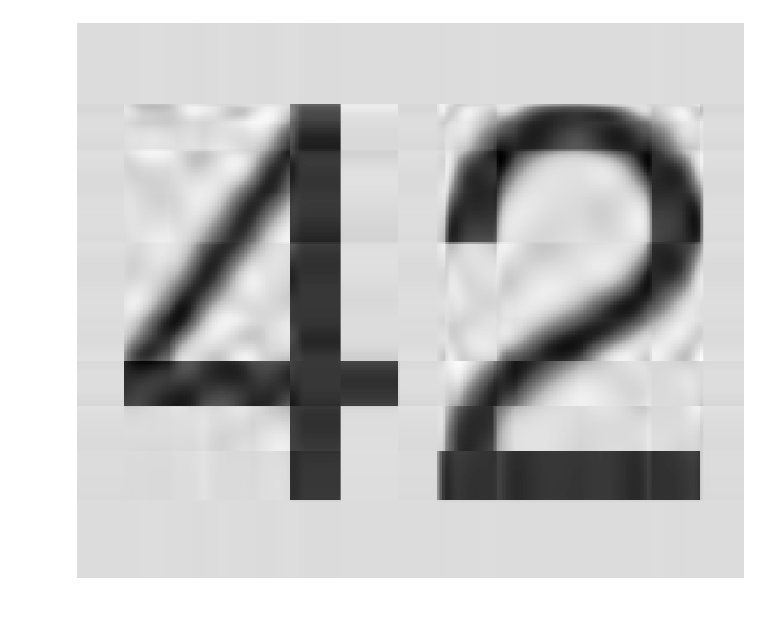
\includegraphics[width=\textwidth]{graphics/svd/42-10.pdf}
        \caption{}
        \label{fig: Theory: SVD-42-10}
    \end{subfigure}
    \caption{
        \subref{fig: Theory: SVD-42-full} An example image of $500\times600=300.000$ pixels.
        \subref{fig: Theory: SVD-42-5} and \subref{fig: Theory: SVD-42-10} Respectively, rank-5 and 10 approximations of the image.
        The low rank approximations are constructed from $5.505$ and $11.010$ parameters, respectively, reduced by a factor of about 56 and 28 compared to the original.
        The high level of structure on the original image results in few large singular values which in turn gives high quality low rank approximations. Note how the axis aligned parts of the ``4" and ``2" are more easily reconstructed.
    }
    \label{fig: Theory: SVD number 42}
\end{figure}
\begin{figure}[tbp!]
    \begin{subfigure}[b]{0.49\textwidth}
        \centering
        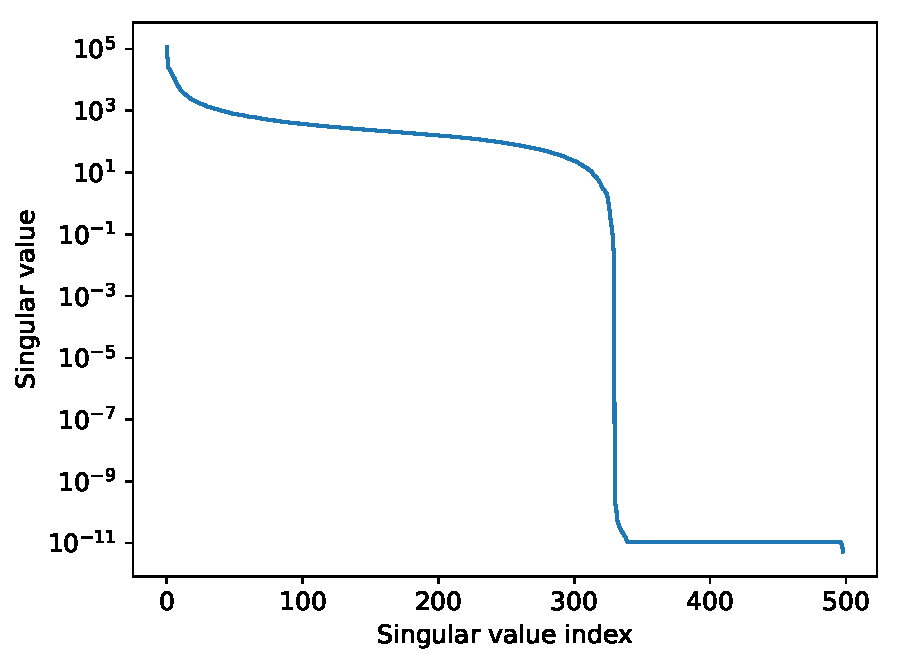
\includegraphics[height=5.7cm]{graphics/svd/42-svds-log.pdf}
        \caption{}
        \label{fig: Theory: SVD-42-svds-log}
    \end{subfigure}
    \hfill
    \begin{subfigure}[b]{0.49\textwidth}
        \centering
        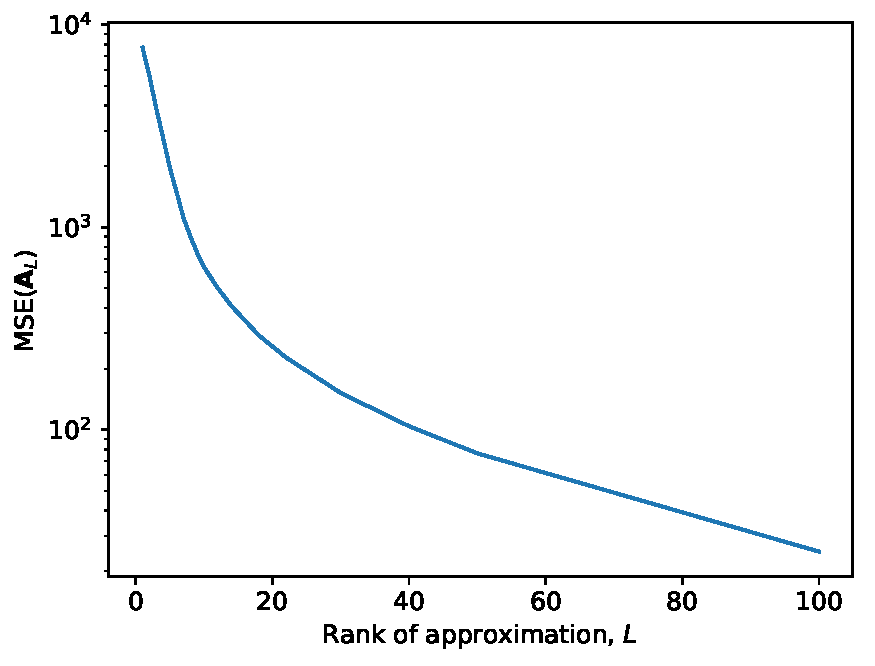
\includegraphics[height=5.7cm]{graphics/svd/42-MSE-log.pdf}
        \caption{}
        \label{fig: Theory: SVD-42-MSE}
    \end{subfigure}
    \caption{
        \subref{fig: Theory: SVD-42-svds-log} Singular values of the image in \autoref{fig: Theory: SVD-42-full} as a function of index.
        \subref{fig: Theory: SVD-42-MSE} \gls{MSE} of different rank approximations of that image.  Note the rapid initial decrease in the singular values driving a steep decrease in the \gls{MSE} over the first $10$ singular values.
    }
    \label{fig: Theory: SVD: singular values and MSE}
\end{figure}

In the context of Gaussian search distributions, the matrix of interest is the covariance matrix which has the additional properties of being symmetric and square and is required to be positive definite. Inspired by the low-rank approximation presented above, a rank-$L$ approximation to the covariance matrix $\Sigmab$ can be written as \cite{Hastie2009}
\begin{equation}
    \Sigmab \approx \D + \sum_{i=1}^L \u_i\u_i\transpose = \D + \U\transpose\U
\end{equation}
where $\u_i$ are $d$ dimensional column vectors and $\U=\bmat{u_1\transpose & \cdots & u_L\transpose}^\text{T}$ has the $\u_i$ vectors in its rows. $\D$ is a diagonal matrix which is chosen large enough that $\Sigmab$ is positive definite. This approximation has $dL$ parameters rather than $d(d+1)/2$ which is considerably fewer for $L\ll d$. 

It seems fair to conjecture that a good approximation might be achievable in this manner for a choice of $L\ll d$ in the case where the search space is the parameter space of an \gls{NN} with $d$ up to hundreds of millions. This thesis has not studied this avenue further.


\subsubsection{Cauchy distribution}
For completeness, this section briefly considers the Cauchy distribution for use in \gls{VO}. Since the Cauchy is a heavy-tailed distribution it can be used for a so-called hill-climber version of \gls{VO} where the population size is 1 \cite{Schaul2011}. 

The \gls{PDF} of the Cauchy is
\begin{equation}
    p(x|\mu,\gamma) = \frac{1}{\pi\gamma}\left[1+\left({\frac{x-\mu}{\gamma}}\right)^{2}\right]^{-1} = \frac{1}{\pi\gamma} \bra{\frac{\gamma ^{2}}{(x-\mu)^{2}+\gamma ^{2}} }
\end{equation}
with log-\gls{PDF}
\begin{equation}
    \log p(x|\mu,\gamma) = - \log(\pi\gamma) - \log\left[1+\left({\frac{x-\mu}{\gamma}}\right)^{2}\right] \ .
\end{equation}
% The gradient of the log-\gls{PDF} is
% \begin{equation}
%     \pderiv{}{x_0}\log p(x|\mu,\gamma) = \frac{2(x-x_0)}{(x-x_0)^2+\gamma^2}
% \end{equation}
% \begin{equation}
%     \pderiv{}{\gamma}\log p(x|\mu,\gamma) = \frac{(x-x_0)^2-\gamma^2}{\gamma\pa{\gamma^2+(x+x_0)^2}} \ .
% \end{equation}
% This is then usable in the \gls{VO} gradient in \eqref{eq: Theory: Variational optimization gradient estimator general search distribution} as the Gaussians. 

At each iteration, a single perturbation is made using the Cauchy and its performance compared to the unperturbed model. If the perturbed model is better it is used as the unperturbed model in the next iteration, otherwise it is disregarded.
Hill-climber \gls{VO} can be better at avoiding getting stuck in local minima. However, due to the rarity of these in the loss surfaces of \glspl{NN} this method is not considered further in this thesis.

%"Making the Cauchy work" introduces the truncated Cauchy which has defined moments \cite{Nadarajah2011}

%\url{https://projecteuclid.org/download/pdfview_1/euclid.bjps/1291387776}

%\todo[inline]{Either write up and include or don't include section on the Cauchy distribution - could be interesting to note Hillclimber version}
%!TEX root = ../Thesis.tex

\section{Natural gradient}\label{sec: Natural Gradient}
This section first discusses the problems related to using the regular search gradient in \gls{VO} in \autoref{sec: Natural Gradient - problems of regular search gradients}. It then discusses how to measure distance or similarity between probability distributions in \autoref{sec: Natural Gradient - The regular gradient and distances between successive search distributions} and and introduces the \gls{KL} divergence in \autoref{sec: Natural Gradient - KL divergence}. The \gls{FIM} is derived in \autoref{sec: Natural Gradient - Fischer information matrix} as a second order approximation to the \gls{KL} divergence. Following this, the natural gradient is derived in \autoref{sec: Natural Gradient: Steepest descent w.r.t. a distance metric} as the optimal search direction when optimizing the variational upper bound subject to a dissimilarity constraint based on the \gls{KL} divergence between the updated and previous search distributions at every iteration of gradient descent. The natural gradient is then computed for the case of a Gaussian search distribution and finally, the benefits of it are demonstrated for a simple problem.
%As discussed in \autoref{sec: Theory: Taylor: Bias and variance of estimator}, the gradient estimators derived so far suffer from a numerical instability for small values of variance while it has been demonstrated that the attainment of such low values is preferred in order to efficiently converge on local/global minima (see \autoref{sec: Variational Optimization: Examples of 1D objective functions optimized with variational optimization}).

\subsection{Problems of regular search gradients}\label{sec: Natural Gradient - problems of regular search gradients}
A central problem of regular search gradients is their inability to precisely locate any optima, even a convex quadratic one. Take for instance a univariate Gaussian to be the search distribution. In order to locate an approximately quadratic optima, $\sigma$ must go to zero in order to place all probability mass at the optimal point, $x^*$. 
However, the search gradients in \eqref{eq: Theory: Variational optimization univariate gaussian search gradients} and the upper bound gradients in \eqref{eq: Theory: Variational optimization univariate gaussian gradient estimators} are not numerically stable for very small values of $\sigma$: As $\sigma\rightarrow0$ clearly $\sfrac{1}{\sigma^2}\rightarrow\infty$ and so does the estimators. Although $\text{E}\left[\epsilon f(x+\epsilon)\right]\rightarrow0$ for $\sigma\rightarrow0$, the variance of the gradient estimator, derived from the Taylor series in \eqref{eq: Theory: Taylor: Variance of univariate gradient}, can be seen to go to infinity.

Thus, the behaviour of \gls{VO} with regular search gradients will be to first adjust $\sigma$ to find a local attractor. When a local attractor has been found, the algorithm steps towards it, gradually decreasing the value of $\sigma$ as the objective function becomes approximately quadratic around the attractor. As $\sigma\rightarrow0$ the gradients become too large and the computed update shoots away from the attractor, effectively restarting the search. Even though not quite as dramatic, the opposite case of $\sigma\gg1$, which would arise at a large plateau, results in insignificant updates to the mean parameter and can completely halt progress \cite{Wierstra2008}.

This behaviour is completely opposite of what is intuitively wanted of a \gls{VO} estimator. When in a flat region, $\sigma$ should be increased and large steps made in any promising direction. When closing in on an attractor, the step sizes should ideally go to zero. This highlights the need for adjusting the gradient to have better numerics for small values of the variance.


\subsection{The distance between successive search distributions}\label{sec: Natural Gradient - The regular gradient and distances between successive search distributions}
The regular gradient is a vector that points in the direction of the steepest increase of the objective function. The steepest direction is understood in terms of Euclidean distance such that the gradient gives the direction where the smallest total change in the parameter gives the largest change in the function value with changes measured by Euclidean distance. It is evident that if Euclidean distance between optimized parameters is not a suitable measure of the resulting variation in the objective function, then the regular gradient gives a suboptimal direction in the search space.

\begin{figure}[tbp!]
    \begin{subfigure}[b]{0.50\textwidth}
        \centering
        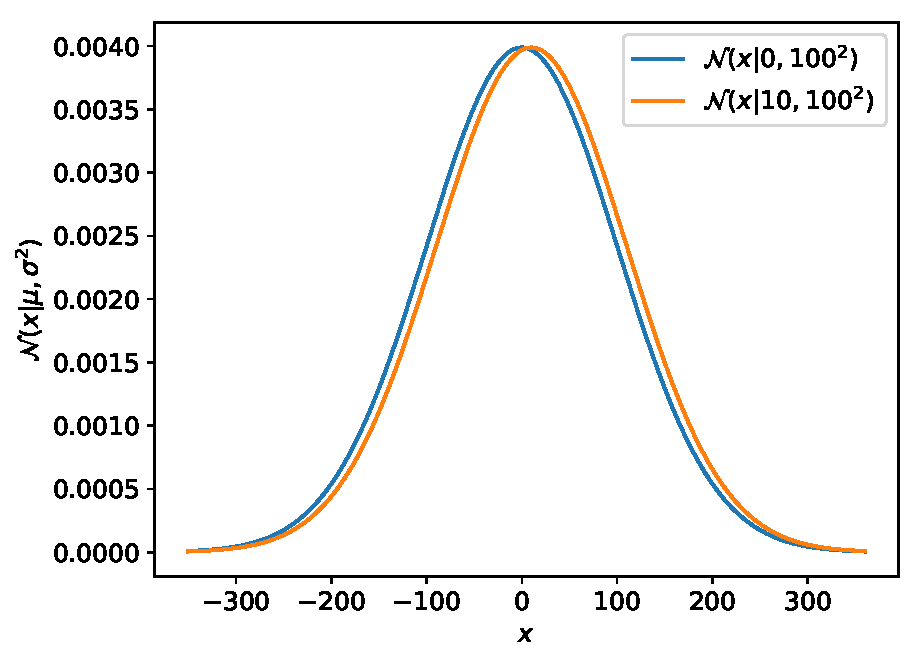
\includegraphics[height=5.2cm]{graphics/gaussian-pdfs/S1.pdf}
        \caption{}
        \label{fig: Theory: gaussian-pdfs/S1}
    \end{subfigure}
    \hfill
    \begin{subfigure}[b]{0.48\textwidth}
        \centering
        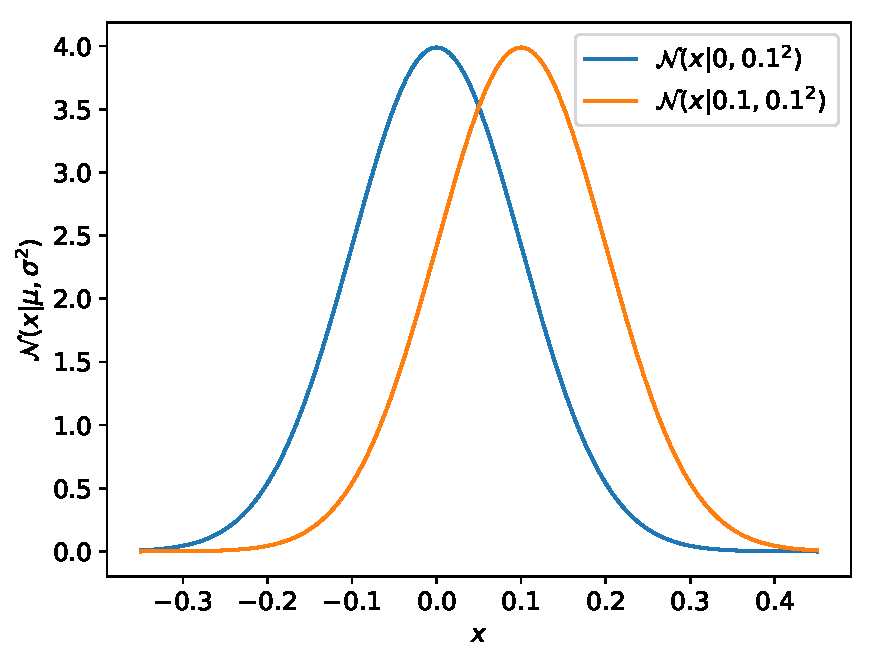
\includegraphics[height=5.2cm]{graphics/gaussian-pdfs/S2.pdf}
        \caption{}
        \label{fig: Theory: gaussian-pdfs/S2}
    \end{subfigure}
    \caption{
        Two pairs of univariate Gaussians, $P_1$ in \subref{fig: Theory: gaussian-pdfs/S1} and $P_2$ in \subref{fig: Theory: gaussian-pdfs/S2}. The $P_1$ pair is obviously very similar while the $P_2$ pair are somewhat dissimilar. A suitable measure of the dissimilarity of two probability distributions is expected to reflect this.
    }
    \label{fig: Theory: gaussian-pdfs}
\end{figure}

In the \gls{VO} setting, a search distribution is maintained over the network weights and it is updated iteratively using gradient descent. Evaluating the closeness of successive search distributions by computing the Euclidean distance between their parameter vectors can be shown to be give counter intuitive results. Take for instance the two pairs of univariate Gaussians shown in \autoref{fig: Theory: gaussian-pdfs},
\begin{align*}
    P_1 &= \cbra{\mathcal{N}(0,100^2), \mathcal{N}(10,100^2)}\\
    \shortintertext{and}
    P_2 &= \cbra{\mathcal{N}(0,0.1^2), \mathcal{N}(0.1,0.1^2)} \ .
\end{align*}
%$$P_1 = \cbra{\mathcal{N}(0,100^2), \mathcal{N}(10,100^2)}$$
%and
%$$P_2 = \cbra{\mathcal{N}(0,0.1^2), \mathcal{N}(0.1,0.1^2)}.$$
Due to their large variance, the first two distributions are almost identical while the other pair of distributions share limited support. As a consequence of their parameterizations however, the Euclidean distance, $D_2$, between the first pair is
$$D_\text{2}\pa{\mathcal{N}(0,100^2), \mathcal{N}(10,100^2)} = \sqrt{\pa{0-10}^2+\pa{100^2-100^2}^2}= 10$$
whereas the distance between the second pair is
$$D_\text{2}\pa{\mathcal{N}(0,0.1^2), \mathcal{N}(0.1,0.1^2)} = \sqrt{\pa{0-0.1}^2+\pa{0.1^2-0.1^2}^2}= 0.1,$$
a factor of 1000 lower. 

That Euclidean distance is an unsuited measure of closeness between probability distributions can be theoretically attributed to distributions not residing in a Euclidean space but rather on a Riemannian manifold (or statistical manifold) \cite{Suzuki2014}. Although this thesis will not delve further into the details of these manifolds, measuring distance within them must be done with respect to a form of distance metric. This is akin to relating a line segment $ds$ in Euclidean space to changes $dx$ and $dy$ in the $x$ and $y$ directions by the relation $ds=\sqrt{dx^2+dy^2}$ only here, $ds$ is a line segment on the statistical manifold and the directions represent parameters of a family of probability distributions, e.g. $\mu$ and $\sigma$ of the univariate Gaussian \cite{Suzuki2014}.


\subsection{The Kullback-Leibler divergence}\label{sec: Natural Gradient - KL divergence}
A better and more natural measure of distance between two probability distributions is the \glsfirst{KL} divergence. It is defined as \cite{Bishop2006}
\begin{align}
    D_\text{KL}(p||q)
    &= -\int p(\x)\log q(\x)\,\text{d}\x - \pa{-\int p(\x)\log p(\x)\,\text{d}\x} \nonumber\\
    &= -\int p(\x)\log\pa{\frac{q(\x)}{p(\x)}}\,\text{d}\x \ .\label{eq: Theory: Definition of KL divergence}
\end{align}
The \gls{KL} divergence satisfies $D_\text{KL}(p||q)\geq0$ with equality only when $p(\x)=q(\x)$ and it is asymmetrical such that $D_\text{KL}(p||q)\ne D_\text{KL}(q||p)$. As such is it strictly speaking not a measure of distance but should rather be interpreted as a measure of information loss by using $q$ rather than $p$ or, inversely, a measure of required additional information by using $q$ rather than $p$, to encode some amount of information. For example, in variational Bayesian methods, the \gls{KL} divergence is often used as the measure of dissimilarity between a distribution $q(\z)$ that approximates a posterior distribution $p(\z|\x)$ where $\x$ and $\z$ are respectively observed and unobserved (latent) variables. In fact, $q(\z)$ approximates Bayes' theorem
\begin{equation}
    p(\z|\x) = \frac{p(\x|\z)p(\z)}{p(\x)}
\end{equation}
in which the marginalization over $\z$ to compute $p(\x)$ is often intractable. The approximation is computed by minimizing the \gls{KL} divergence of the approximate posterior between the true posterior, $D_\text{KL}(q||p)$. The \gls{KL} divergence can then be seen as the average minimal additional amount of information required to specify the value of $\z$ as a result of using $q(\z)$ instead of $p(\z|\x)$\footnote{The information content is measured in bits if the base 2 logarithm is used and in nats if the natural logarithm is used. The relation between the two is $\SI{1}{nat}=\frac{1}{\ln 2}\si{bit} \approx \SI{1.44}{bit}$.} \cite{Bishop2006}.

A symmetrized version of the \gls{KL} divergence which satisfies $D_\text{KL}(p,q)=D_\text{KL}(q,p)$ can be defined as
\begin{align}
    D_\text{KL}(p,q)
    &= D_\text{KL}(p||q) + D_\text{KL}(q||p) \nonumber\\
    &= -\int p(\x)\log\pa{\frac{q(\x)}{p(\x)}}\,\text{d}\x - \int q(\x)\log\pa{\frac{p(\x)}{q(\x)}}\,\text{d}\x \nonumber\\
    &= \int p(\x)\log\pa{\frac{p(\x)}{q(\x)}}\,\text{d}\x - \int q(\x)\log\pa{\frac{p(\x)}{q(\x)}}\,\text{d}\x \nonumber\\
    &= \int \pa{p(\x)-q(\x)}\log\pa{\frac{p(\x)}{q(\x)}}\,\text{d}\x \ .\label{eq: Theory: Definition of symmetrized KL divergence}
\end{align}

The \gls{KL} divergence and the symmetrized \gls{KL} divergence between two univariate Gaussians, $\mathcal{N}(\mu_1,\sigma_1^2)$ and $\mathcal{N}(\mu_2,\sigma_2^2)$, are\footnote{For derivations, see \autoref{app: Regular and symmetrized Kullback-Leibler divergence for univariate Gaussian}}
\begin{align}
    D_\text{KL}\pa{\mathcal{N}(\mu_1,\sigma_1^2) || \mathcal{N}(\mu_2,\sigma_2^2)} &= \log\pfrac{\sigma_2}{\sigma_1} + \frac{\sigma_1^2+(\mu_1+\mu_2)^2}{2\sigma_2^2} - \frac{1}{2}\\
    D_\text{KL}\pa{\mathcal{N}(\mu_1,\sigma_1^2), \mathcal{N}(\mu_2,\sigma_2^2)} &= \pa{(\mu_1-\mu_2)^2 + (\sigma_1^2 + \sigma_2^2)}\pa{\frac{1}{2\sigma_1^2} + \frac{1}{2\sigma_2^2}} - 2 \ .
\end{align}
For the pairs, $P_1$ and $P_2$ considered above, the \gls{KL} divergence and symmetrized \gls{KL} divergence become
\begin{align}
    D_\text{KL}\pa{\mathcal{N}(0,100^2)||\mathcal{N}(10,100^2)} &= 0.005\nonumber\\
    D_\text{KL}\pa{\mathcal{N}(0,0.1^2)||\mathcal{N}(0.1,0.1^2)} &= 0.5\nonumber
\end{align}
and
\begin{align}
    D_\text{KL}\pa{\mathcal{N}(0,100^2), \mathcal{N}(10,100^2)} &= 0.01\nonumber\\
    D_\text{KL}\pa{\mathcal{N}(0,0.1^2), \mathcal{N}(0.1,0.1^2)} &= 1\nonumber \ ,
\end{align}
respectively. The ordering of the distributions in the regular \gls{KL} divergence is unimportant in this specific case since the asymmetry is in the variances and the variances are equal here. In both cases, this measure of dissimilarity is a factor of $100$ lower for the $P_1$ pair compared to the $P_2$ pair. Evidently, both the regular and symmetrized \gls{KL} divergence much better represent similarity between distributions than the Euclidean measure which, contrary to intuition, considered the $P_1$ pair to be much further apart than $P_2$.


\subsection{The Fisher information matrix}\label{sec: Natural Gradient - Fischer information matrix}
For the purposes of the following section, this section will consider how to compute an approximation to the \gls{KL} divergence.
For two distributions, $p(\x|\thetab)$ and $p(\x|\thetab+\Delta\thetab)$, that differ by some small vector $\Delta\thetab$ in their parameter vectors, a second order Taylor approximation to their symmetric \gls{KL} divergence can be computed as follows\footnote{This is derivation is intended to sketch the proof but is not a completely rigorous proof in itself.}. Let
$$\Delta p(\x|\thetab)=p(\x|\thetab+\Delta\thetab)-p(\x|\thetab)$$
and rewrite the symmetric \gls{KL} divergence as follows
\begin{align}
    D_\text{KL}(p(\x|\thetab+\Delta\thetab),p(\x|\thetab))
    &= \int \pa{p(\x|\thetab+\Delta\thetab)-p(\x|\thetab)}\log\pa{\frac{p(\x|\thetab+\Delta\thetab)}{p(\x|\thetab)}}\,\text{d}\x\nonumber\\
    &= \int \Delta p(\x|\thetab)\log\pa{1+\frac{\Delta p(\x|\thetab)}{p(\x|\thetab)}}\,\text{d}\x\nonumber\\
    &= \int p(\x|\thetab)\frac{\Delta p(\x|\thetab)}{p(\x|\thetab)}\log\pa{1+\frac{\Delta p(\x|\thetab)}{p(\x|\thetab)}}\,\text{d}\x \ .
\end{align}
Now, the Taylor expansion of the logarithm is
\begin{equation}
    \log (1+x) = \log(1) + x + \mathcal{O}(x^2)
    %\log (1+x) = \log(1) + x + \frac{1}{2}x^2 + \frac{1}{3}x^3 + \dots,
\end{equation}
which implies that
\begin{equation}
    \log\pa{1+\frac{\Delta p(\x|\thetab)}{p(\x|\thetab)}} \approx \frac{\Delta p(\x|\thetab)}{p(\x|\thetab)} \ .
\end{equation}
Applying this to the symmetric \gls{KL} divergence above yields
\begin{equation}
    D_\text{KL}p(\x|\thetab)(p(\x|\thetab+\Delta\thetab),p(\x|\thetab)) \approx \int p(\x|\thetab) \frac{\Delta p(\x|\thetab)}{p(\x|\thetab)}\frac{\Delta p(\x|\thetab)}{p(\x|\thetab)}\,\text{d}\x \ .
\end{equation}
Given that the parameter change $\Delta\thetab$ is small enough, $\nabla_\thetab p(\x|\thetab)\transpose\Delta\thetab$ will be a finite difference approximation to $\Delta p(\x|\thetab)$, i.e.
\begin{equation}
    \Delta p(\x|\thetab) \approx \nabla_\thetab p(\x|\thetab)\transpose\Delta\thetab \ .
\end{equation}
Substituting this approximation and using the log-derivative trick \eqref{eq: Theory: Log-derivative trick for pdf}, the symmetric \gls{KL} divergence becomes
\begin{align}
    D_\text{KL}(p(\x|\thetab+\Delta\thetab),p(\x|\thetab))
    % &\approx \int p(\x|\thetab)\bra{
    % \Delta\thetab\transpose\frac{\nabla_\thetab p(\x|\thetab)}{p(\x|\thetab)}}\bra{
    % \frac{\nabla_\thetab p(\x|\thetab)\transpose}{p(\x|\thetab)}\Delta\thetab}\,\text{d}\x\nonumber\\
    &\approx \int p(\x|\thetab)
    \Delta\thetab\transpose\frac{\nabla_\thetab p(\x|\thetab)}{p(\x|\thetab)}
    \frac{\nabla_\thetab p(\x|\thetab)\transpose}{p(\x|\thetab)}\Delta\thetab\,\text{d}\x\nonumber\\
    &= \int p(\x|\thetab)
    \Delta\thetab\transpose\nabla_\thetab\log p(\x|\thetab)
    \nabla_\thetab\log p(\x|\thetab)\transpose\Delta\thetab\,\text{d}\x\nonumber\\
    &= \Delta\thetab\transpose\int p(\x|\thetab)
    \nabla_\thetab\log p(\x|\thetab)
    \nabla_\thetab\log p(\x|\thetab)\transpose\,\text{d}\x\; \Delta\thetab \ .
\end{align}
Note that the integral is an expectation with respect to $p(\x|\thetab)$ of the outer product of the gradient of the log-\gls{PDF} of the search distribution. This can be seen to be the \glsfirst{FIM} which is defined as \cite{Bishop2006}
\begin{equation}\label{eq: Theory: Fischer information matrix definition}
    \F_\thetab
    = \text{E}\bra{\nabla_\thetab\log p(\x|\thetab)\nabla_\thetab\log p(\x|\thetab)\transpose}_{p(\x|\thetab)} \ .
\end{equation}
Using the \gls{FIM}, the approximate symmetric \gls{KL} divergence can thus be written as
\begin{equation}\label{eq: Theory: Second order approximation to the symmetric KL divergence}
    D_\text{KL}(p(\x|\thetab+\Delta\thetab),p(\x|\thetab)) \approx \Delta\thetab\transpose\F_\thetab\Delta\thetab \ .
\end{equation}
Under certain regularity conditions which will not be discussed here, the \gls{FIM} can also be written as \cite{Ly2017}
\begin{equation}\label{eq: Theory: Fischer information matrix definition (for computation)}
    \F_\thetab = - \text{E}\bra{\H_\thetab\log p(\x|\thetab)} = \text{Cov}\bra{\nabla_\thetab\log p(\x|\thetab)}
\end{equation}
which is useful for computation.


\subsection{Steepest descent w.r.t. a distance metric}\label{sec: Natural Gradient: Steepest descent w.r.t. a distance metric}
\autoref{sec: Natural Gradient} set out to understand what makes the regular gradient suboptimal for gradient descent in \glsfirst{VO}. Now that it is clear why Euclidean distance is unsuited and the \gls{KL} divergence has been introduced and substantiated as a more fitting measure of similarity between distributions, this section will derive the natural gradient by imposing a constraint on the dissimilarity between the updated and previous search distributions. To demonstrate the relation between the regular and natural gradients, the regular gradient will be derived first in an unconstrained manner and by imposing a Euclidean dissimilarity constraint.

At each iteration of \gls{VO}, a direction $\Delta\thetab$ is sought that minimizes the variational upper bound. With no constraints on the update this can be expressed as the following unconstrained minimization problem.
\begin{equation}\label{eq: Theory: Unconstrained VO optimization problem at each iteration}
    \min_{\Delta\thetab} U(\thetab+\Delta\thetab) \approx U(\thetab) + \nabla_\thetab U(\thetab)\transpose\Delta\thetab + \frac{1}{2}\Delta\thetab\transpose\H_\thetab U(\thetab)\transpose\Delta\thetab \ ,
\end{equation}
which uses a second order Taylor expansion of the variational upper bound around the current parameter $\thetab$. The solution to this problem is found by taking the gradient w.r.t. $\Delta\thetab$ of the objective,
\begin{equation}
    \nabla_{\Delta\thetab}\bra{U(\thetab) + \nabla_\thetab U(\thetab)\transpose\Delta\thetab + \frac{1}{2}\Delta\thetab\transpose\nabla_\thetab U(\thetab)\transpose\Delta\thetab} = \nabla_\thetab U(\thetab) + \H_\thetab U(\thetab)\Delta\thetab,
\end{equation}
setting it to zero and solving for $\Delta\thetab$. This yields
\begin{equation*}
    \Delta\thetab = -\H_\thetab U(\thetab)^{-1}\nabla_\thetab U(\thetab)
\end{equation*}
which is the well-known Newton search direction. In cases where Hessian information is not available or computationally intractable, it can be ignored and a fixed learning rate used on the gradient instead giving the search direction
\begin{equation}
    \Delta\thetab = -\eta\nabla_\thetab U(\thetab) \ .
\end{equation}

Alternatively, a constraint can be imposed on the optimization problem in \eqref{eq: Theory: Unconstrained VO optimization problem at each iteration}. For instance, constraining the Euclidean distance $D_2(\cdot)$ between parameters $\thetab$ and $\thetab+\Delta\thetab$ to be some small constant $\kappa^2$, the problem becomes,
\begin{equation}\label{eq: Theory: Constrained VO optimization problem at each iteration (Euclidean dissimilarity)}
    \begin{aligned}
        \min_{\Delta\thetab} &\; U(\thetab+\Delta\thetab) \approx U(\thetab) + \nabla_\thetab U(\thetab)\transpose\Delta\thetab\\
        \text{subject to} &\; D_2(\thetab+\Delta\thetab, \thetab) = \sqrt{\Delta\thetab\transpose\Delta\thetab} = \kappa^2 \ ,
    \end{aligned}
\end{equation}
where only a first order Taylor approximation has been used since second order dependencies are introduced in the constraint. Such a problem is solved using the methods of constrained optimization \cite{Nocedal2006}. Writing the Euclidean constraint as $\Delta\thetab\transpose\Delta\thetab = \kappa$, the Lagrangian for the problem becomes
\begin{equation}
    \mathcal{L}(\thetab,\lambda) = U(\thetab) + \nabla_\thetab U(\thetab)\transpose\Delta\thetab - \lambda\pa{\Delta\thetab\transpose\Delta\thetab - \kappa}
\end{equation}
which is minimized w.r.t. $\Delta\thetab$
\begin{equation*}
    0 = \nabla_{\Delta\thetab}\mathcal{L}(\thetab,\lambda) = \nabla_\thetab U(\thetab) - \lambda\Delta\thetab
\end{equation*}
yielding
\begin{equation}
    \Delta\thetab = \lambda^{-1}\nabla_\thetab U(\thetab) \ .
\end{equation}
The Lagrange multiplier $\lambda$ can be found by first forming the dual of the Lagrangian by insertion of the result into the primal Lagrangian and then minimizing the dual w.r.t. the multiplier. The dual Lagrangian becomes
\begin{align}
    \mathcal{L}_d(\lambda)
    &= U(\thetab) + \lambda^{-1}\nabla_\thetab U(\thetab)\transpose\nabla_\thetab U(\thetab) - \lambda\kappa\nonumber\\
    &= U(\thetab) + \lambda^{-1}\nabla^2_\thetab U(\thetab) - \lambda\kappa\nonumber
\end{align}
where $\nabla^2$ denotes the vector Laplacian. Differentiate the Lagrangian w.r.t. $\lambda$ and set it to zero,
\begin{equation*}
    0 = \frac{d}{d\lambda}\mathcal{L}_d(\lambda) = -\lambda^{-2}\nabla^2_\thetab U(\thetab) - \kappa \ .
\end{equation*}
Finally solve for $\lambda$ to obtain
\begin{equation}
    \lambda = - \sqrt{\frac{\nabla^2_\thetab U(\thetab)}{\kappa}} \ .
\end{equation}
The search direction then becomes
\begin{equation}
    \Delta\thetab = - \sqrt{\frac{\kappa}{\nabla^2_\thetab U(\thetab)}}\nabla_\thetab U(\thetab) = -\eta\nabla_\thetab U(\thetab)
\end{equation}
where $\eta=\sqrt{\frac{\kappa}{\nabla^2_\thetab U(\thetab)}}$ is some potentially undesirable learning rate that can be replaced by a constant without changing the search direction. Note that this constrained approach has resulted in the emergence of the negative regular gradient as the optimal descent direction for minimization while constraining step sizes to be constant in the sense of Euclidean distance.

Rather than using the Euclidean distance between distribution parameters as the measure of dissimilarity between the distributions, now the approximate symmetrized \gls{KL} divergence defined in \eqref{eq: Theory: Definition of symmetrized KL divergence} is used to impose the dissimilarity constraint in \eqref{eq: Theory: Constrained VO optimization problem at each iteration (Euclidean dissimilarity)}. The minimization problem is then given by,
\begin{equation}\label{eq: Theory: Constrained VO optimization problem at each iteration (KL divergence dissimilarity)}
    \begin{aligned}
        \min_{\Delta\thetab} &\; U(\thetab+\Delta\thetab) \approx U(\thetab) + \nabla_\thetab U(\thetab)\transpose\Delta\thetab\\
        \text{subject to} &\; D_\text{KL}\pa{p(\x|\thetab+\Delta\thetab), p(\x|\thetab)} \approx \frac{1}{2}\Delta\thetab\transpose\F_\thetab\Delta\thetab = \kappa \ ,
    \end{aligned}
\end{equation}
where $p(\x|\thetab)$ is the used search distribution.
As discussed earlier, the dissimilarity constraint now takes the form of a distance w.r.t. a distance metric, here, the \gls{FIM}. In fact, the \gls{FIM} measures closeness of the shape of two distributions and is proportional to the amount of information that the distribution function contains about the parameter. As such, it provides a distance metric on the statistical manifold \cite{Suzuki2014}.
Again, to obtain the optimal search direction, the Lagrangian is formed,
\begin{equation}
    \mathcal{L}(\thetab,\lambda) = U(\thetab) + \nabla_\thetab U(\thetab)\transpose\Delta\thetab - \lambda\pa{\frac{1}{2}\Delta\thetab\transpose\F_\thetab\Delta\thetab - \kappa} \ ,
\end{equation}
differentiated w.r.t. $\Delta\thetab$ and set equal to zero,
\begin{equation}
    0 = \nabla_\thetab\mathcal{L}(\thetab,\lambda) = \nabla_{\Delta\thetab} U(\thetab) - \lambda\F_\thetab\Delta\thetab \ ,
\end{equation}
and finally solved for $\Delta\thetab$ to yield
\begin{equation}
    \Delta\thetab = \lambda^{-1}\F_\thetab^{-1}\nabla_\thetab U(\thetab) \ .
\end{equation}
Again, the Lagrange multiplier $\lambda$ can be found by minimizing the dual Lagrangian,
\begin{equation}
    \mathcal{L}_d(\lambda) = U(\thetab) + \lambda^{-1} \nabla_\thetab U(\thetab)\transpose\F_\thetab^{-1}\nabla_\thetab U(\thetab) - \lambda\kappa \ ,
\end{equation}
w.r.t the multiplier,
\begin{equation}
    0 = \frac{d}{d\lambda}\mathcal{L}_d(\lambda) = -\lambda^{-2} \nabla_\thetab U(\thetab)\transpose\F_\thetab^{-1}\nabla_\thetab U(\thetab) - \kappa \ ,
\end{equation}
and solving for $\lambda$,
\begin{equation}
    \lambda = -\sqrt{\frac{\nabla_\thetab U(\thetab)\transpose\F_\thetab^{-1}\nabla_\thetab U(\thetab)}{\kappa}} \ .
\end{equation}
The search direction is then
\begin{equation}
    \Delta\thetab = -\sqrt{\frac{\kappa}{\nabla_\thetab U(\thetab)\transpose\F_\thetab^{-1}\nabla_\thetab U(\thetab)}}\F_\thetab^{-1}\nabla_\thetab U(\thetab) = -\eta\F_\thetab^{-1}\nabla_\thetab U(\thetab)
\end{equation}
where $\eta=\sqrt{\frac{\kappa}{\nabla_\thetab U(\thetab)\transpose\F_\thetab^{-1}\nabla_\thetab U(\thetab)}}$ is an arbitrary learning rate as before. This search direction is the optimal direction of descent for minimization of the objective while satisfying the constraint that the updated distribution is dissimilar from the previous distribution only by a constant amount as measured by the symmetric \gls{KL} divergence. This search direction is precisely the natural gradient originally introduced in \cite{Amari1998}.

The natural gradient is thus computed by rescaling the regular gradient with the inverse \gls{FIM}. Since the \gls{FIM} is a positive semi-definite matrix it has $n(n+1)/2$ unique entries for a distribution with $n$ parameters. This can in some cases be intractable to store and compute. For example, for an \gls{NN} optimized with \gls{VO} using a $d$-dimensional multivariate Gaussian with full covariance matrix $n=(d+d(d+1)/2)=\mathcal{O}(d^2)$ and the number of elements in the \gls{FIM} is $\mathcal{O}(d^4)$. 
% , the number of parameters in the \gls{FIM} may be as high as
% $$(d+d(d+1)/2)(d+d(d+1)/2) = \frac{1}{4}(d^2 + 3d)^2$$
% which scales as $\mathcal{O}(d^4)$. 
However, in some interesting special cases, the \gls{FIM} has much fewer unique parameters. Below, such distributions are considered. 

In \cite{Wierstra2008}, an additional abstraction is made for a general class of rotationally symmetric distributions (which includes the Gaussian) by introduction of ``exponential local natural coordinates". This constitutes a reparameterization of the search distribution that results in the \gls{FIM} becoming the identity and the gradient thus automatically being the natural one. This has not been considered further here but could reduce computation when using the natural gradient with distributions with e.g. covariances.

\iffalse
\textbf{- Steepest Descent with Respect to a Metric N derived by minimizing objective while keeping distance to new parameters equal to constant}
- \url{http://www.ias.tu-darmstadt.de/uploads/Research/Thesis/thesiP_1.pdf} page 75 for solution of minimization of distance between probability distributions.

% http://people.missouristate.edu/songfengzheng/Teaching/MTH541/Lecture%20notes/Fisher_info.pdf
% https://en.wikipedia.org/wiki/Fisher_information

\cite{Peters2007}

\url{https://hips.seas.harvard.edu/blog/2013/01/25/the-natural-gradient/}

\url{http://kvfrans.com/what-is-the-natural-gradient-and-where-does-it-appear-in-trust-region-policy-optimization/}

Natural gradient introduced by \cite{Amari1998}

Wierstra Natural Evolution Strategies \cite{Wierstra2008}


\begin{align}
    D_\text{KL}(p_\thetab||p_{\thetab+\Delta\thetab})
    &= D_\text{KL}(\Delta\thetab)\\
    &\approx D_\text{KL}(0) + \Delta\thetab\transpose\nabla_\thetab D_\text{KL}(0) + \frac{1}{2}\Delta\thetab\transpose\nabla^2_\thetab D_\text{KL}(0)\Delta\thetab\\
    &= 0 + (0?) + Something Fischer matrix kinda\\ 
    &= D_\text{KL}(p_\thetab||p_{\thetab})\\
    &= NEED CALCULATIONS HERE\\
    &= \frac{1}{2}\Delta\thetab\transpose\bra{\int p_\thetab(\x)\nabla^2_\thetab\log p_\thetab(\x)\transpose\,\text{d}\x}\Delta\thetab\\
    &= \frac{1}{2}\Delta\thetab\transpose\bra{-\int p_\thetab(\x)\nabla_\thetab\log p_\thetab(\x)\nabla_\thetab\log p_\thetab(\x)\,\text{d}\x}\Delta\thetab\\
    &= \frac{1}{2}\Delta\thetab\transpose\F_\thetab\Delta\thetab
\end{align}
\fi


\subsection{Natural gradient for different search distributions}
This section derives the \gls{FIM} and the associated natural gradient for the univariate, isotropic and separable Gaussian search distributions.


\subsubsection{Univariate Gaussian}
The \gls{FIM} for a univariate Gaussian can be computed as follows. Since the univariate Gaussian has two parameters, the \gls{FIM} will be a $2\times2$ matrix. The derivatives of the Gaussian log-\gls{PDF} were computed in \eqref{eq: Theory: Variational optimization univariate gaussian search gradients} with which the gradient of the univariate Gaussian w.r.t. to its parameter vector $\thetab=\bmat{\mu & \sigma^2}^\text{T}$ can be constructed as
\begin{equation}
    \nabla_\thetab\log\mathcal{N}(x|\mu,\sigma^2) = \bmat{\frac{1}{\sigma^2}(x-\mu) \\ -\frac{1}{2\sigma^2}+\frac{1}{2\sigma^4(x-\mu)^2}} \ .
\end{equation}
Its Hessian is then
\begin{equation}
    \H_\thetab\log\mathcal{N}(x|\mu,\sigma^2) = \bmat{-\frac{1}{\sigma^2} & -\frac{1}{\sigma^4}(x-\mu) \\ -\frac{1}{\sigma^4}(x-\mu) & \frac{1}{2\sigma^4}-\frac{1}{\sigma^6}(x-\mu)^2} \ .
\end{equation}
With $\text{E}\bra{x-\mu}=0$ and $\text{E}\bra{(x-\mu)^2}=\sigma^2$ and using \eqref{eq: Theory: Fischer information matrix definition (for computation)}, the \gls{FIM} then becomes
\begin{equation}
    \F_\thetab = -\text{E}\bra{\H_\thetab\log\mathcal{N}(x|\mu,\sigma^2)} = \bmat{\frac{1}{\sigma^2} & 0 \\ 0 & \frac{1}{2\sigma^4}}
\end{equation}
and the inverse \gls{FIM} required for the natural gradient is easily obtained,
\begin{equation}
    \F_\thetab^{-1} = \bmat{\sigma^2 & 0 \\ 0 & 2\sigma^4} \ .
\end{equation}
The natural gradient version of the \gls{VO} gradient estimator in \eqref{eq: Theory: Variational optimization univariate gaussian gradient estimators} therefore becomes
\begin{equation}
    \begin{aligned}
        \sigma^2\pderiv{}{\mu}U(\mu,\sigma^2) &= \sigma\text{E}\bra{f(\mu + \sigma\epsilon)\epsilon} \approx \frac{\sigma}{N}\sum_{n=1}^N f(\mu+\sigma\epsilon_n)\epsilon_n\\
        2\sigma^4\pderiv{}{\sigma^2}U(\mu,\sigma^2) &= \sigma^2\text{E}\bra{f(\mu + \sigma\epsilon)\left(\epsilon^2-1\right)} \approx \frac{\sigma^2}{N}\sum_{n=1}^N f(\mu + \sigma\epsilon_n)\left(\epsilon_n^2-1\right)\\
    \end{aligned}\label{eq: Theory: Variational optimization univariate gaussian gradient estimators (natural gradient)}
\end{equation}
where $\epsilon\sim\mathcal{N}(0,1)$. These evidently posses the desired property that the gradient goes to zero as the variance goes to zero and the opposite.


\subsubsection{Isotropic Gaussian}
A $d$-dimensional isotropic Gaussian, $\mathcal{N}(\mub,\sigma^2\I)$, has $d+1$ parameters which implies that the \gls{FIM} will be a $(d+1)\times(d+1)$ matrix. The gradients of the log-\gls{PDF} of the isotropic Gaussian were derived in \eqref{eq: Theory: Variational optimization multivariate isotropic gaussian search gradients}. 
The gradient of the isotropic Gaussian w.r.t. to its parameter vector $\thetab=\bmat{\mub & \sigma^2}^\text{T}$ can then be constructed as
\begin{equation}
    \nabla_\thetab\log\mathcal{N}(\x|\mub,\sigma^2\I) = \bmat{\frac{1}{\sigma^2}(\x-\mub) \\ -\frac{d}{2\sigma^2} + \frac{1}{2\sigma^4}(\x-\mub)\transpose(\x-\mub)} \ .
\end{equation}
It follows that the Hessian is
\begin{equation}
    \H_\thetab\log\mathcal{N}(\x|\mub,\sigma^2\I) = \bmat{-\frac{1}{\sigma^2}\I & -\frac{1}{\sigma^4}(\x-\mub) \\ -\frac{1}{\sigma^4}(\x-\mub) & \frac{d}{2\sigma^4}-\frac{1}{\sigma^6}(\x-\mub)\transpose(\x-\mub)} \ .
\end{equation}
Again, use \eqref{eq: Theory: Fischer information matrix definition (for computation)} to compute the \gls{FIM} and exploit that $\text{E}\bra{\x-\mub}=\0$ and $\text{E}\bra{(\x-\mub)\transpose(\x-\mub)}=d\sigma^2$ to obtain\footnote{This follows from the following argument.
\begin{align}
    \text{E}\bra{(\x-\mub)\transpose(\x-\mub)} = \text{E}\bra{\x\transpose\x}-\text{E}\bra{\x\transpose\mub}-\text{E}\bra{\mub\transpose\x}+\text{E}\bra{\mub\transpose\mub}
    = \text{E}\bra{\x\transpose\x} - \mub\transpose\mub \ .\nonumber
\end{align}
Now, when $\x\sim\mathcal{N}(\mu,\sigma^2\I)$
\begin{align}
    \text{E}\bra{\x\transpose\x} &= \text{E}\bra{\sum_{i=1}^d x_i^2}
    = \sum_{i=1}^d \text{E}\bra{x_i^2}
    = \sum_{i=1}^d \text{Var}\bra{x_i}+\text{E}\bra{x_i}^2
    = \sum_{i=1}^d \sigma^2+\mu_i^2
    = d\sigma^2+\mub\transpose\mub\nonumber \ ,
\end{align}
such that
\begin{align}
    \text{E}\bra{(\x-\mub)\transpose(\x-\mub)} &= d\sigma^2\nonumber \ .
\end{align}
}
\begin{equation}
    \F_\thetab = \bmat{\frac{1}{\sigma^2}\I & 0 \\ 0 & \frac{1}{2\sigma^4}} \Longleftrightarrow \F_\thetab^{-1} = \bmat{\sigma^2\I & 0 \\ 0 & 2\sigma^4} \ .
\end{equation}
%The inverse \gls{FIM} required for the natural gradient is easily obtained,
% \begin{equation}
%     \F_\thetab^{-1} = \bmat{\sigma^2\I & 0 \\ 0 & 2\sigma^4}.
% \end{equation}
This is simply the univariate result in each dimension of the mean while the result for the scalar variance parameter remains unchanged.
The natural gradient version of the \gls{VO} gradient estimator in \eqref{eq: Theory: Variational optimization multivariate isotropic gaussian gradient estimators} therefore becomes
\begin{equation}
    \begin{aligned}
        \sigma^2\nabla_\mub U(\mub,\sigma^2) &= \sigma\text{E}\bra{f(\mub + \sigma\epsilonb)\epsilonb} \approx \frac{\sigma}{N}\sum_{n=1}^N f(\mub+\sigma\epsilonb_n)\epsilonb_n\\
        2\sigma^4\nabla_{\sigmab^2} U(\mub,\sigma^2) &= \sigma^2\text{E}\bra{f(\mub + \sigma\epsilonb)\left(\epsilonb\transpose\epsilonb-d\right)} \approx \frac{\sigma^2}{N}\sum_{n=1}^N f(\mub + \sigma\epsilonb_n)\left(\epsilonb_n^2-d\right)\\
    \end{aligned}\label{eq: Theory: Variational optimization multivariate isotropic gaussian gradient estimators (natural gradient)}
\end{equation}
where $\epsilon\sim\mathcal{N}(\0,\I)$. The transformation applied to the \gls{VO} gradient using the isotropic Gaussian is clearly identical to the one applied to the gradient using a univariate Gaussian; in both cases the mean and variance gradients are multiplied by the scalars $\sigma^2$  and $2\sigma^4$, respectively.



\subsubsection{Separable Gaussian}
A $d$-dimensional separable Gaussian, $\mathcal{N}\pa{\x|\mub, (\sigmab^2\e\transpose)\odot\I}$, has $2d$ parameters which implies that the \gls{FIM} will be a $2d\times2d$ matrix. The gradients of the log-\gls{PDF} of the separable Gaussian were derived in \eqref{eq: Theory: Variational optimization multivariate isotropic gaussian search gradients (mub)} and \eqref{eq: Theory: Variational optimization multivariate isotropic gaussian search gradients (sigmab^2)}.
The gradient of the separable Gaussian w.r.t. its parameter vector $\thetab=\bmat{\mub & \sigmab^2}^\text{T}$ can then be constructed as
\begin{equation}
    \nabla_\thetab\log\mathcal{N}\pa{\x|\mub, (\sigmab^2\e\transpose)\odot\I} = \bmat{\sigmab^{-2} \odot (\x-\mub) \\  -\frac{1}{2}\sigmab^{-2} + \frac{1}{2} \sigmab^{-4}\odot(\x-\mub)^2} \ .
\end{equation}
It follows that the Hessian is
\begin{equation}
    \H_\thetab\log\mathcal{N}\pa{\x|\mub, (\sigmab^2\e\transpose)\odot\I} = \bmat{\sigmab^{-2} \odot\I & -\sigmab^{-4}\odot(\x-\mub) \\ -\sigmab^{-4}\odot(\x-\mub) & \frac{1}{2}\sigmab^{-4}-\sigmab^{-6}\odot(\x-\mub)^2} \ .
\end{equation}
Again, use \eqref{eq: Theory: Fischer information matrix definition (for computation)} to compute the \gls{FIM} and exploit that $\text{E}\bra{\x-\mub}=\0$ and $\text{E}\bra{(\x-\mub)^2}=\sigmab^2$ to obtain
\begin{equation}
    \F_\thetab = \bmat{\sigmab^{-2}\odot\I & 0 \\ 0 & \frac{1}{2}\sigmab^{-4}\odot\I} \Longleftrightarrow \F_\thetab^{-1} = \bmat{\sigmab^{2}\odot\I & 0 \\ 0 & 2\sigmab^{4}\odot\I} \ .
\end{equation}
% and, due to $F_{\thetab}$ being diagonal,
% \begin{equation}
%     \F_\thetab^{-1} = \bmat{\sigmab^{2}\odot\I & 0 \\ 0 & 2\sigmab^{4}\odot\I}.
% \end{equation}
Once again, this is the univariate result in each dimension of the parameter vector of the separable Gaussian. The natural gradient version of the \gls{VO} gradient estimator in \eqref{eq: Theory: Variational optimization separable gaussian gradient estimators} therefore becomes
\begin{equation}
    \begin{aligned}
        \sigmab^{2}\odot\nabla_\mub U(\mub,\sigma^2) &= \sigmab\odot\text{E}\bra{f(\mub + \sigmab\odot\epsilonb)\epsilonb}\\
        &\approx \sigmab\odot\frac{1}{N}\sum_{n=1}^N f(\mub+\sigmab\odot\epsilonb_n)\epsilonb_n\\
        2\sigmab^{4}\odot\nabla_\sigma^2 U(\mub,\sigma^2) &= \sigmab^{2}\odot\text{E}\bra{f(\mub + \sigmab\odot\epsilonb)\pa{\epsilonb^2 - 1}}\\
        &\approx \sigmab^{2}\odot\frac{1}{N}\sum_{n=1}^N f(\mub + \sigmab\odot\epsilonb_n)\pa{\epsilonb_n^2 - 1}\\
    \end{aligned}\label{eq: Theory: Variational optimization separable gaussian gradient estimators (natural gradient)}
\end{equation}
where $\epsilon\sim\mathcal{N}(\0,\I)$. The transformation applied here is again similar to the one applied to the gradient using a univariate Gaussian.


%If any two parameters, $\theta_i$ and $\theta_j$ are independent, the \gls{FIM} will contain a zero at the $(i,j)$'th entry, i.e. $\F_{ij}=0$. Clearly then if all parameters are independent, the \gls{FIM} will be diagonal.

% \subsection{Natural gradient for Cauchy search distributions}
% \begin{equation}
%     f(x;x_{0},\gamma )={\frac  {1}{\pi \gamma \left[1+\left({\frac{x-x_{0}}{\gamma}}\right)^{2}\right]}}=\frac{1}{\pi \gamma }\left[\frac{\gamma ^{2}}{ (x-x_{0})^{2}+\gamma ^{2}}\right],
% \end{equation}
% Since the Cauchy distribution has undefined moments, the Fischer information matrix is undefined in this case. However 
% \url{https://projecteuclid.org/download/pdfview_1/euclid.bjps/1291387776}

% Relation to CMA-ES \cite{Hansen2016} and TR-CMA-ES \cite{Abdolmaleki2017} as related methods that are more heuristic and less principled.

% \todo[inline]{Write section on natural gradient for Cauchy distribution (only if included earlier and useful)}



\subsection{Comparison of regular and natural gradients}\label{sec: Natural Gradient: Comparison of regular and natural gradients}
\begin{figure}[tbp!]
    \begin{subfigure}[b]{0.49\textwidth}
        \centering
        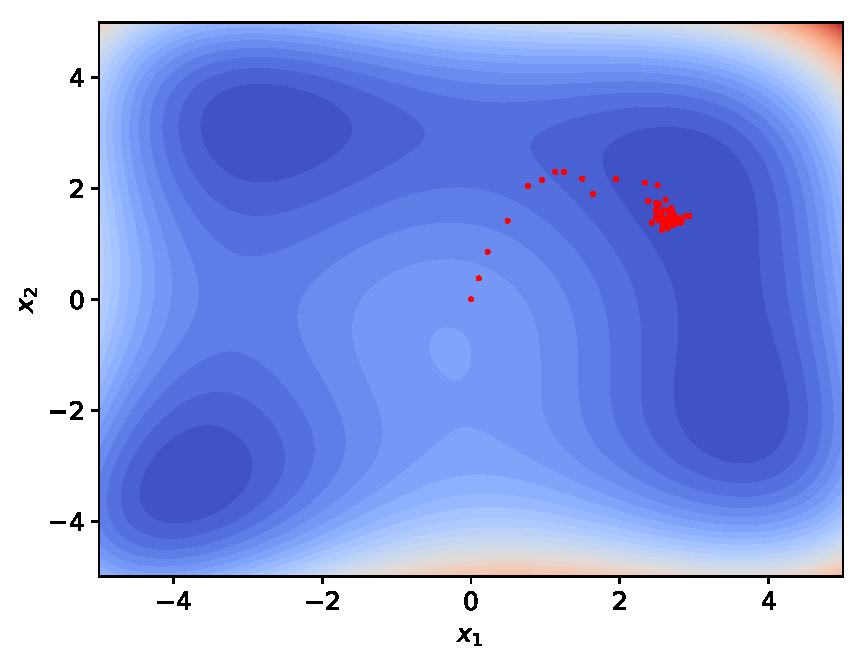
\includegraphics[height=5.8cm]{graphics/var-opt-conv/ES-himmelblau-convergence.pdf}
        \caption{}
        \label{fig: Theory: var-opt-conv-ES-himmelblau-convergence}
    \end{subfigure}
    \hfill
    \begin{subfigure}[b]{0.49\textwidth}
        \centering
        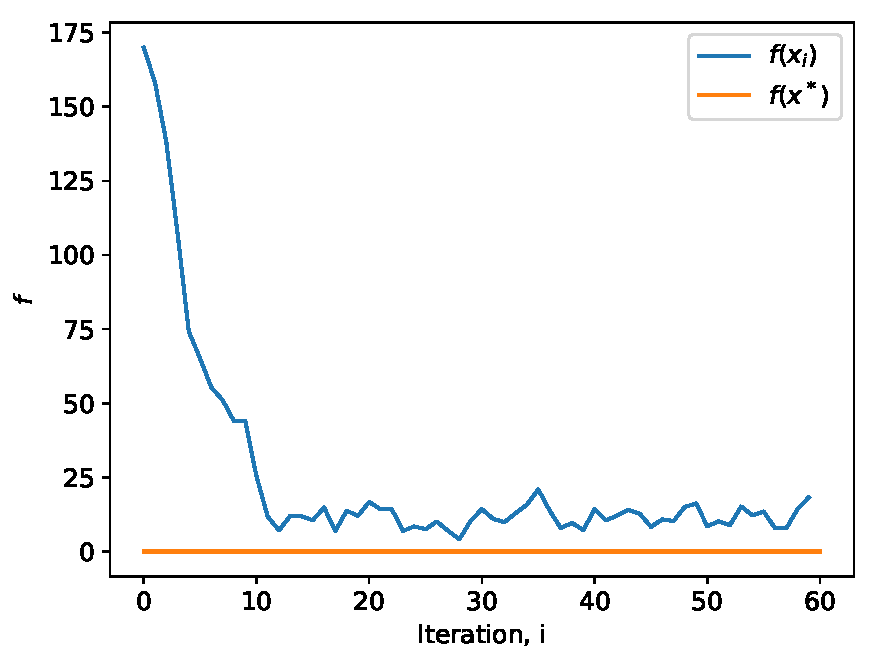
\includegraphics[height=5.8cm]{graphics/var-opt-conv/ES-himmelblau-f.pdf}
        \caption{}
        \label{fig: Theory: var-opt-conv-ES-himmelblau-f}
    \end{subfigure}
    \caption{\subref{fig: Theory: var-opt-conv-ES-himmelblau-convergence} Convergence on Himmelblau's function of the algorithm used by \cite{Salimans2017} with no adaptation of the variance. As in earlier contours, red denotes high values, blue denotes low values and the darker the colour, the higher the absolute value. The actual values are omitted for simplicity. \subref{fig: Theory: var-opt-conv-ES-himmelblau-f} Objective function value at each iteration of the algorithm. The algorithm finds a minimum but struggles to converge due to the fixed search distribution variance.}
    \label{fig: Theory: var-opt-conv-ES-himmelblau}
\end{figure}
In Figures \ref{fig: Theory: var-opt-conv-ES-himmelblau}, \ref{fig: Theory: var-opt-conv-VO-R-himmelblau} and \ref{fig: Theory: var-opt-conv-VO-N-himmelblau}, different versions of the variational optimization algorithm listed in \autoref{alg: Canonical variational optimization} are compared on Himmelblau's function. Himmelblau's function is two-dimensional objective function with four global minima and a local maximum. In these figures as before, red denotes high values, blue denotes low values and the darker the colour, the higher the absolute value. The actual values are omitted for simplicity.


In \autoref{fig: Theory: var-opt-conv-ES-himmelblau}, the convergence of the algorithm used in \cite{Salimans2017} and derived in \eqref{eq: Theory: Taylor: Multivariate gradient estimate from standard Gaussian} is shown. This algorithm estimates the regular gradient and does not adapt the value of the Gaussian search distribution variance. In \subref{fig: Theory: var-opt-conv-ES-himmelblau-convergence}, the iteration sequence is plotted on the contours of the objective function while in \subref{fig: Theory: var-opt-conv-ES-himmelblau-f}, the corresponding objective function value at each iteration is shown along with the global minimum value. Evidently, this algorithm quickly homes in on one of the global minima and stays in its vicinity for succeeding iterations. The objective function value reaches low values, but the fixed size of the variance results in it fluctuating above the global minimum never converging on it.

\autoref{fig: Theory: var-opt-conv-VO-R-himmelblau} presents the convergence of the \gls{VO} algorithm using an isotropic Gaussian search distribution. The used estimators for the regular gradients of the mean and variance are those in \eqref{eq: Theory: Variational optimization multivariate isotropic gaussian gradient estimators}. Similarly to the fixed variance version, this algorithm also quickly homes in on a minimum. However, the optimization of the variance results in increasingly smaller variances for each iteration. As previously discussed and and as expected, this increasingly smaller variance can be seen to give rise to increasingly larger gradient estimates. In the limit of zero variance (close to the minimum), the gradients explode and the function value starts increasing.

Finally, \autoref{fig: Theory: var-opt-conv-VO-N-himmelblau} presents the convergence of the same \gls{VO} algorithm using instead the natural gradient. The \gls{VO} natural gradient estimators for the univariate Gaussian used here are those in \eqref{eq: Theory: Variational optimization univariate gaussian gradient estimators (natural gradient)}. The minimum is found as before but this time the optimization of the variance drives the gradients to zero at the minimum resulting in much better convergence. Although the direction of the natural gradient is not different from the regular gradient for this specific type of search distribution, the gradient is much more well-behaved as $\sigma$ decreases.

These examples clearly demonstrate the differences between the methods and highlights \gls{VO} with natural gradients as the best choice for this problem. Replacing the regular gradient with the natural gradient results in better numerics for the estimators and convergence to the minimum. It should however be noted that Himmelblau's function is a low-dimensional objective function and the number of perturbations is much larger than the dimensionality for this example. This is fundamentally different from the optimization of \glspl{NN} by search in the extremely high-dimensional parameter space.

It can be noted that Gaussian \gls{VO} with fixed variance as in \autoref{fig: Theory: var-opt-conv-ES-himmelblau} in fact optimizes for the expected fitness of the entire population of perturbations rather than the fitness of the search distribution center \cite{Lehman2017}. As such, the fitness of the center of the search distribution (the unperturbed individual) may not be optimal at all although it often is close to the optimum, at least in terms of search space distance. This also results in solutions that exhibit robustness to small perturbations to the parameters \cite{Lehman2017}.
\begin{figure}[tbp!]
    \begin{subfigure}[b]{0.49\textwidth}
        \centering
        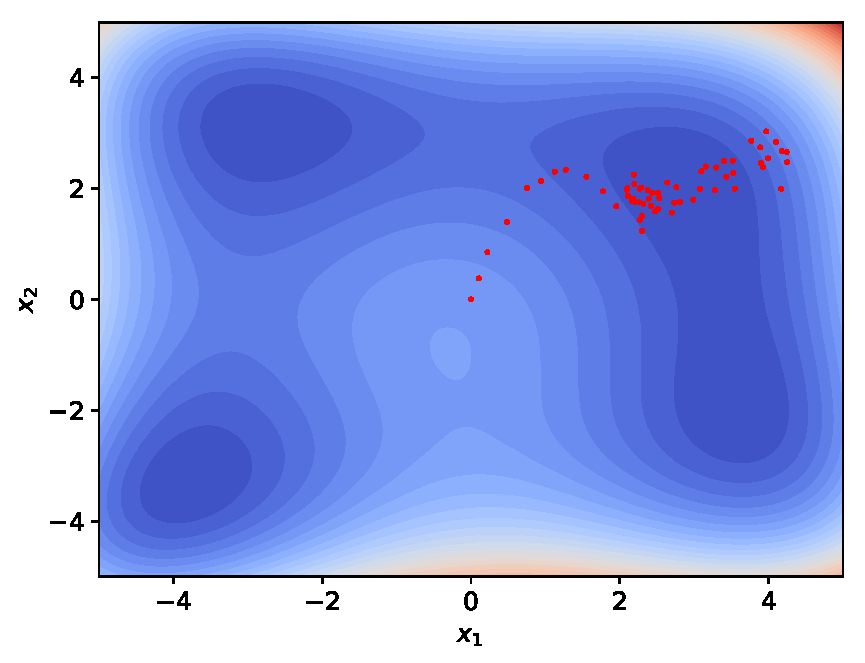
\includegraphics[height=5.8cm]{graphics/var-opt-conv/VO-R-himmelblau-convergence.pdf}
        \caption{}
        \label{fig: Theory: var-opt-conv-VO-R-himmelblau-convergence}
    \end{subfigure}
    \hfill
    \begin{subfigure}[b]{0.49\textwidth}
        \centering
        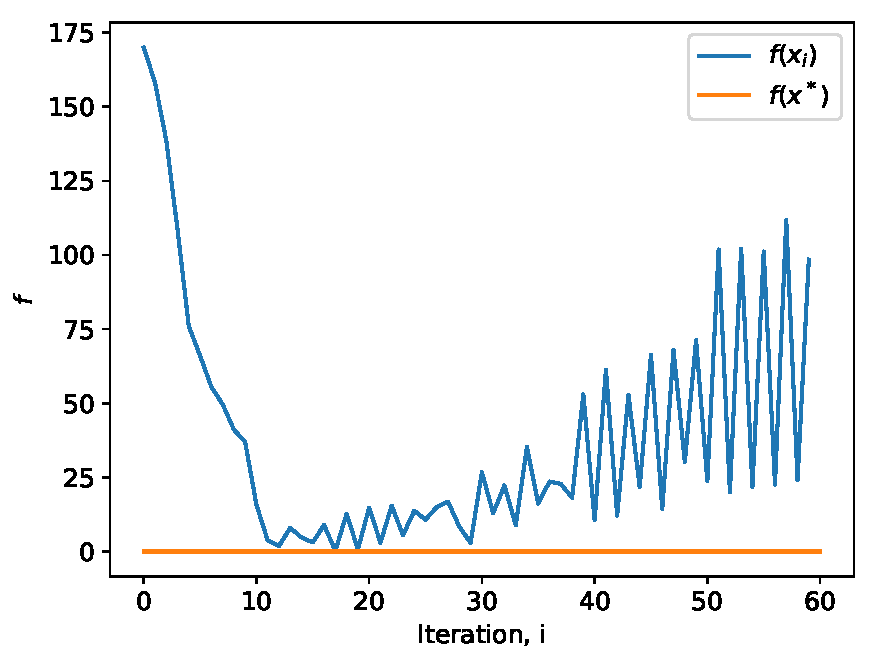
\includegraphics[height=5.8cm]{graphics/var-opt-conv/VO-R-himmelblau-f.pdf}
        \caption{}
        \label{fig: Theory: var-opt-conv-VO-R-himmelblau-f}
    \end{subfigure}
    \caption{\subref{fig: Theory: var-opt-conv-VO-R-himmelblau-convergence} Convergence of the \gls{VO} algorithm with isotropic Gaussian search distribution using regular gradients. \subref{fig: Theory: var-opt-conv-VO-R-himmelblau-f} Objective function value at each iteration. Similarly to the fixed variance version, a minimum is found, but the optimization of the variance drives it towards zero, resulting in larger gradients and instability.}
    \label{fig: Theory: var-opt-conv-VO-R-himmelblau}
\end{figure}
\begin{figure}[tbp!]
    \begin{subfigure}[b]{0.49\textwidth}
        \centering
        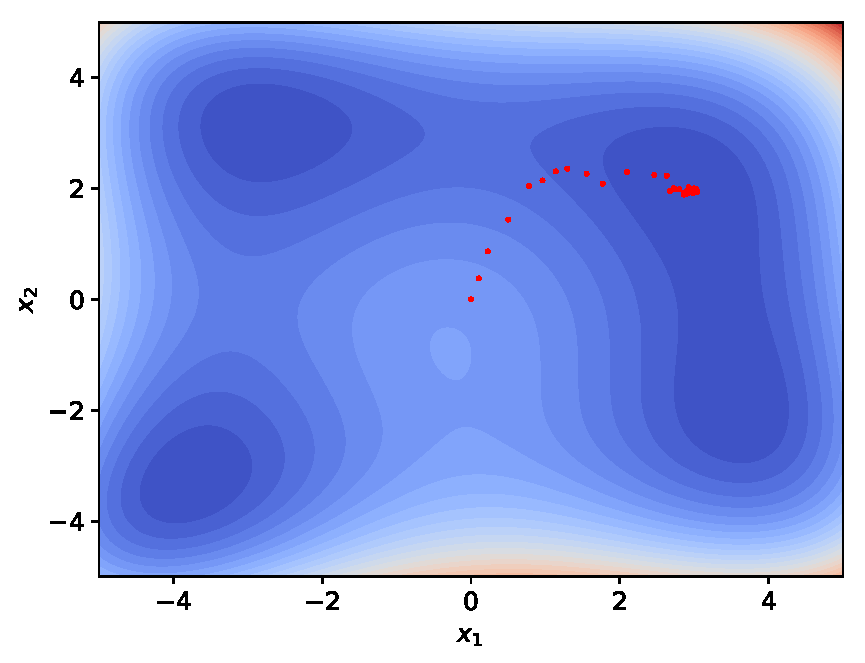
\includegraphics[height=5.8cm]{graphics/var-opt-conv/VO-N-himmelblau-convergence.pdf}
        \caption{}
        \label{fig: Theory: var-opt-conv-VO-N-himmelblau-convergence}
    \end{subfigure}
    \hfill
    \begin{subfigure}[b]{0.49\textwidth}
        \centering
        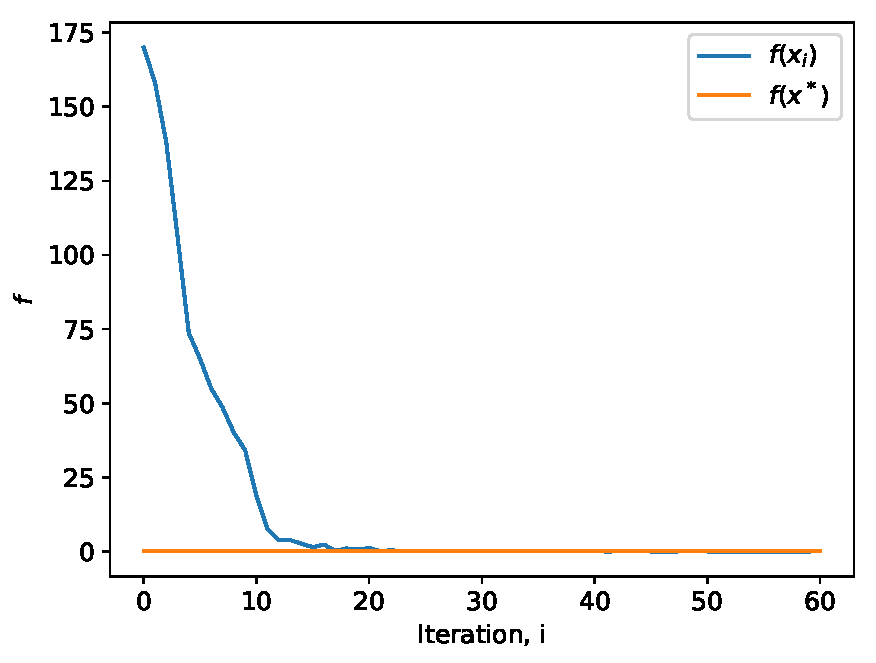
\includegraphics[height=5.8cm]{graphics/var-opt-conv/VO-N-himmelblau-f.pdf}
        \caption{}
        \label{fig: Theory: var-opt-conv-VO-N-himmelblau-f}
    \end{subfigure}
    \caption{\subref{fig: Theory: var-opt-conv-VO-N-himmelblau-convergence} Convergence of the \gls{VO} algorithm with isotropic Gaussian search distribution using natural gradients. \subref{fig: Theory: var-opt-conv-VO-N-himmelblau-f} Objective function value at each iteration. A minimum is found and the optimization of the variance drives the gradients toward zero resulting in convergence to the optimum.}
    \label{fig: Theory: var-opt-conv-VO-N-himmelblau}
\end{figure}
%!TEX root = ../Thesis.tex

\section{Performance and robustness improving techniques}\label{sec: Theory: Performance and robustness improving techniques}

\subsection{Fitness rank transform}\label{sec: Theory: Performance and robustness improving techniques: Fitness rank transform}
\begin{figure}[tbp!]
    \begin{subfigure}[b]{0.485\textwidth}
        \centering
        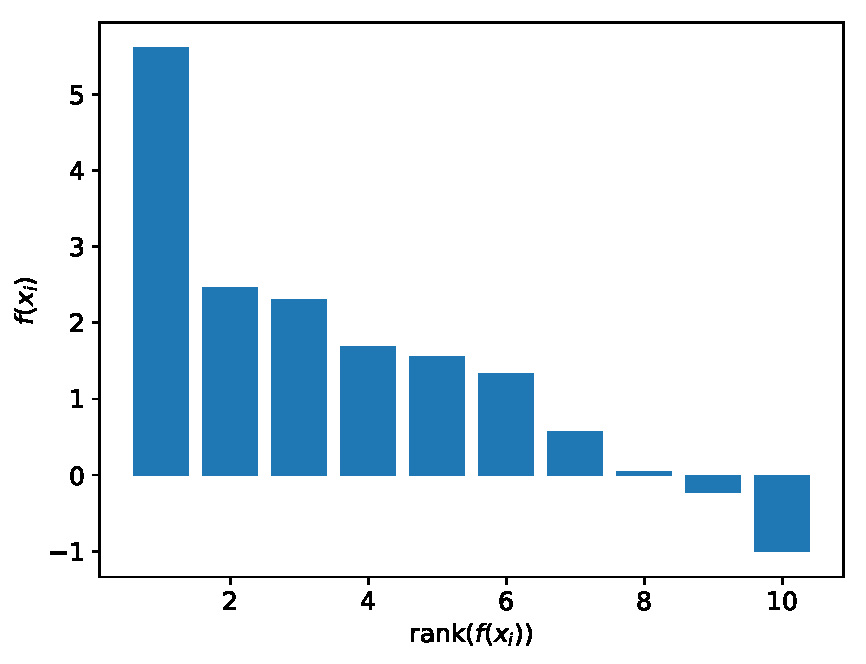
\includegraphics[height=5.8cm]{graphics/fitness-transform/fitnesses.pdf}
        \caption{}
        \label{fig: Theory: fitness-transform/fitnesses.pdf}
    \end{subfigure}
    \hfill
    \begin{subfigure}[b]{0.495\textwidth}
        \centering
        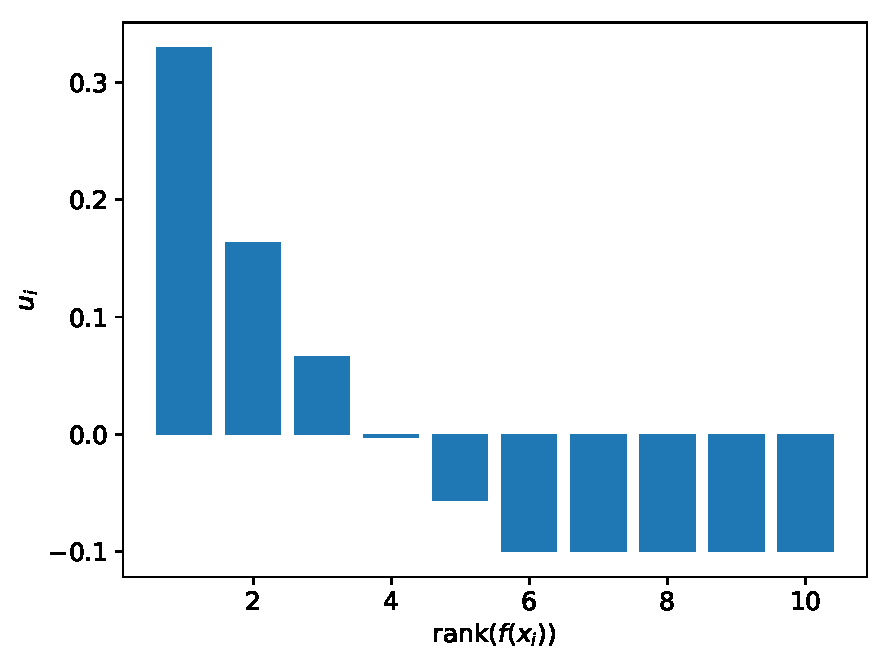
\includegraphics[height=5.8cm]{graphics/fitness-transform/transform.pdf}
        \caption{}
        \label{fig: Theory: fitness-transform/transform.pdf}
    \end{subfigure}
    \caption{
        Illustration of the fitness rank transform applied to evaluated fitnesses.
        \subref{fig: Theory: fitness-transform/fitnesses.pdf} Ten randomly sampled fitnesses. 
        \subref{fig: Theory: fitness-transform/transform.pdf} The ten corresponding utilities according to \eqref{eq: Theory: Fitness rank transform}.
    }
    \label{fig: Theory: fitness-transform}
\end{figure}
In general, the values returned by the function being optimized, $f(\x_i)$, may vary wildly in size depending on the function and the points at which it is sampled. Directly using the returned function value makes hyperparameters, such as the learning rate, highly dependent on the objective function. Additionally, the returned function values may increase or decrease considerably as the algorithm converges to an optimum. Clearly, this can result in numerical instability and hyperparameters being highly dependent on the objective function is undesirable.

One way to avoid this is to transform the function values before they are used to compute the gradient. One possible transform type is the so-called rank transform. 
This transform ranks the sampled function values $f(\x_i)$ and assigns to each one a value that depends only the relative value of the sample compared to the other samples. These new values are called utilities.
Utilities do not change in size during optimization and have no dependency on the actual value of the objective function but do encode information on the relative fitness of the samples. Replacing thge function values by utlities makes \gls{VO} invariant to any order-preserving transformation of the objective function such as addition or multiplication by a scalar \cite{Wierstra2008}. To decouple the learning rate of the algorithm from the utilities it is appropriate to require that $\sum_{i=1}^N \size{u_i} = C$ for some constant $C$.

Several possible choices of rank transform exist and it should be viewed as a free parameter of the problem. In this thesis, the same fitness rank transform as used in \cite{Wierstra2008} has been applied throughout. This is also closely related to the one used in the \gls{CMA-ES} \cite{Hansen2001}. This transformation requires sorting the fitnesses $f(\x_i)$ descending order such that $\x_1$ denotes the best sample and $\x_N$ the worst. The associated fitnesses are then replaced by the utilities given by
\begin{equation}\label{eq: Theory: Fitness rank transform}
    u_i = \frac{\max\cbra{0, \log\pa{\frac{N}{2}+1}-\log\pa{k}}}{\sum_{j=1}^N\max\cbra{0, \log\pa{\frac{N}{2}+1}-\log\pa{j}}} - \frac{1}{N} \ ,\quad i=1,\dots,N \ ,
\end{equation}
such that $u_i$ replaces $f(\x_i)$. \autoref{fig: Theory: fitness-transform} shows the the transformation of ten randomly sampled fitnesses in \subref{fig: Theory: fitness-transform/fitnesses.pdf} to their corresponding utilities in \subref{fig: Theory: fitness-transform/transform.pdf} using \eqref{eq: Theory: Fitness rank transform}.






\subsection{Importance mixing}\label{sec: Theory: Importance mixing}
First introduced in \cite{Sun2009} and explored further in \cite{Yi2009} and \cite{Schaul2011a}, importance mixing is a probabilistic approach to decrease the number of new samples necessary to estimate the search distribution gradient at each iteration and is closely related to importance sampling \cite{Goodfellow2016}. Importance mixing exploits the fact that the \gls{VO} algorithm maintains a search distribution of candidate solutions to include previous perturbations into the next iteration based on how likely they are under the new search distribution.

\subsubsection{Procedure}
Specifically, since the search distribution is only every updated in small steps, the \gls{KL} divergence between the current distribution, $p(\epsilonb|\thetab)$, and the previous one, $p(\x|\thetab')$, will always be relatively small\footnote{This is even more true when using the natural gradient as discussed in \autoref{sec: Natural Gradient}}. This results in many perturbations sampled from $p(\x|\thetab)$ being located in high density areas of $p(\epsilonb|\thetab')$. In turn, this leads to fitness evaluations being unnecessarily repeated \cite{Sun2009}.

Importance mixing seeks to solve this problem by the following algorithm. First, perform rejection sampling on the previous search distribution, $p(\x|\thetab')$, such that perturbation $\epsilonb_i$ is accepted for reuse with probability
\begin{equation}
    \min\cbra{1, (1-\alpha)\frac{p(\epsilonb_i)|\thetab)}{p(\epsilonb_i)|\thetab')}}
\end{equation}
where $\alpha\in\bra{0,1}$ is the forced minimal refresh rate. The more likely the perturbation is in the new distribution compared to the old, the higher the acceptance probability. This leads to the acceptance of $N_a\geq0$ perturbations. Second, perform reverse rejection sampling of perturbations from the current search distribution, $\epsilonb_j\sim p(\epsilonb|\thetab)$ accepting the perturbations with probability
\begin{equation}
    \max\cbra{\alpha, 1 - \frac{p(\epsilonb_j)|\thetab')}{p(\epsilonb_j)|\thetab)}}
\end{equation}
until a $N-N_a$ perturbations have been accepted resulting in a total sample size of $N$. This procedure is listed in \autoref{alg: Importance mixing}. In the extreme, setting $\alpha=1$ results in no perturbations being accepted in the first step and all perturbations being accepted in step two. This is effectively the same as not using importance mixing. It can be noted that since the reused samples are likely in the new search distribution, they must also be some of the better performing samples of the previous iteration, assuming that the search distribution was updated in a promising direction.

In \cite{Sun2009} this algorithm is shown to yield a new set of samples that conform to the current search distribution, $p(\epsilonb|\thetab)$. Furthermore, \cite{Yi2009} shows empirically that the number of new fitness evaluations in an iteration was reduced by a factor of 5 for a range of black box optimization benchmarks. 

\begin{algorithm}[tbp!]
    \caption{Importance mixing \cite{Sun2009}. \label{alg: Importance mixing}}
    \begin{algorithmic}[1]
        \Require{Search distributions; current, $p(\epsilonb|\thetab)$, and previous, $p(\epsilonb|\thetab')$. $N$ previous perturbations, $\epsilonb_i\sim p(\epsilonb|\thetab')$. Forced minimal refresh rate, $\alpha$.}
        \For{each previous perturbation $i=1,\dots,N$}
            \State Compute importance weight 
            $$\frac{p(\epsilonb_i|\thetab)}{p(\epsilonb_i|\thetab')}$$
            \State Accept $\epsilonb_i$ for reuse with probability
            $$\min\cbra{1, (1-\alpha)\frac{p(\epsilonb_i|\thetab)}{p(\epsilonb_i|\thetab')}}$$
        \EndFor
        \State Let $N_a$ be the number of perturbations accepted for reuse.
        \Repeat{\;with $j=1,\dots$}
            \State Sample new perturbation $\epsilonb_j\sim p(\epsilonb|\thetab)$
            \State Accept $\epsilonb_j$ with probability
            $$\max\cbra{\alpha, 1 - \frac{p(\epsilonb_j|\thetab')}{p(\epsilonb_j|\thetab)}}$$
        \Until{$N-N_a$ new perturbations have been accepted}\\
        \Return the total set of perturbations $\{\epsilonb_i, \epsilonb_j\}$ for all accepted $i$ and $j$.
    \end{algorithmic}
\end{algorithm}


\subsubsection{Previous work and dimensionality}
To the author's best knowledge, importance mixing has been applied along with \gls{VO} mostly to ordinary black box function optimization and only to very small \glspl{NN}, such as an \gls{RNN} with 21 weights optimized to solve the pole balancing task \cite{Yi2009}. The recent application of a \gls{VO} variant to neural networks in \cite{Salimans2017} did not reuse any previous samples, always creating new ones at every iteration.

Considering search space dimensionality, the previous applications of importance mixing correspond to the case where the number of samples is larger than the number of dimensions, $N>d$. In this case, the problem solved by importance mixing is the redundant sampling of the objective function. Importance mixing then works by sampling from the new distribution while reusing samples from the distribution of the previous iteration. The resulting total set of samples then conforms to the new distribution while having a reduced number of new samples to evaluate. Using importance mixing thus decreases the number of required function evaluations. The number of search distribution parameter updates (gradient estimates) is not lowered by use of importance mixing.

However, when the search space dimensionality is much higher than the number of samples, $N\ll d$, importance mixing can be interpreted from another perspective as well. Recall the discussion on dimensionality of \autoref{sec: Theory: Variational optimization: Remarks on dimensionality}. Here it was noted that when $N\ll d$, the $N$ samples span an $N$ dimensional subspace of the $d$ dimensional search space. Reusing samples from the previous iteration(s) then corresponds to reusing the most promising subspace dimensions from the previous iteration for the new search.


\subsubsection{High-dimensional importance weight collapse}
Notwithstanding the promises of importance mixing, as many other techniques and algorithms, it suffers from the curse of dimensionality. The issue arises as a consequence of the high dimension of the samples and their associated search distributions. Specifically, the importance weights collapse for high dimensional density functions since they have practically disjoint support\footnote{The support of a real-valued function is the subset of the domain outside of which the function is equal to zero\cite{Christensen2010}. Two sets are said to be disjoint if they have no elements in common. Disjoint support of two densities then means that whenever one density produces a nonzero output, the other produces a zero.} \cite{Bengtsson2008}. In practice this results in the importance weights being zero or in rare cases practically infinite in turn removing the random element of the rejection sampling. This makes importance mixing unsuited for high-dimensional spaces; at least without modifications. \autoref{fig: Theory: importance_mixing/importance_weights_boxplot} illustrates the high-dimensional importance weight collapse.

Obvious methods for addressing the problem of high-dimensionality are those of dimensionality reduction. Dimensionality reduction in the weight space of \glspl{NN} naturally hints towards indirect encondings. Examples are those developed for neuroevolution applications in \cite{Stanley2009} and \cite{Koutnik2016}. 
Another approach to the dimensionality reduction is that developed in \cite{Sugiyama2010} which specifically aims at improving density ratio estimation by performing estimation in the so-called hetero-distributional subspace which can be low-dimensional. Yet another way of reducing the dimensionality of the search space of \glspl{NN} is to consider the activations rather than the weights and then map activation gradients to weight gradients. The number of activations is typically much smaller than the number of weights. In a regular \gls{FNN}, the transformation between two layers with respectively $n_1$ and $n_2$ activations has a total of $n_1+n_2$ activations and $n_1n_2$ weights potentially with $n_2$ biases. For large enough values of $n_1$ and $n_2$, $n_1+n_2\ll n_1n_2$, although the activation space dimension is still rather high for most \gls{NN} models.
%This approach was taken in the development of variational dropout \cite{Kingma2015a} which uses the so-called ``local reparameterization trick" to reduce the variance of a stochastic gradient by removing within batch covariance.
Circumventing the importance weight collapse in the context of \gls{VO} could give potentially significant speedups due to reuse of information and fewer required function evaluations.
% \todo[inline]{Is it possible to use some other measure of closeness?? Perhaps $\norm{\mub-\epsilonb}/\norm{\sigmab}$??}
% \todo[inline]{Add references to sections doing this, if any}

Importance sampling has seen other applications within deep learning. In \cite{Zhao2014} and \cite{Alain2015} it was used to form an alternative to uniform sampling of training data during \gls{SGD} that focuses on the most informative parts of the training data in order to reduce gradient variance. In \cite{Katharopoulos2017} and \cite{Katharopoulos2018} these ideas were further developed and \cite{Katharopoulos2018} finds relative test error reductions of between 5 and 17\% using this technique for image classification. 
In \cite{Katharopoulos2017}, a surrogate \gls{NN} was trained to predict approximate importance weights during training of a primary task \gls{NN}.
%The relatively small dimensionality of the input space allowed  to train a small surrogate \gls{NN} to predict approximate importance weights during training of the primary task network.

\begin{figure}[tbp!]
    \begin{subfigure}[b]{0.485\textwidth}
        \centering
        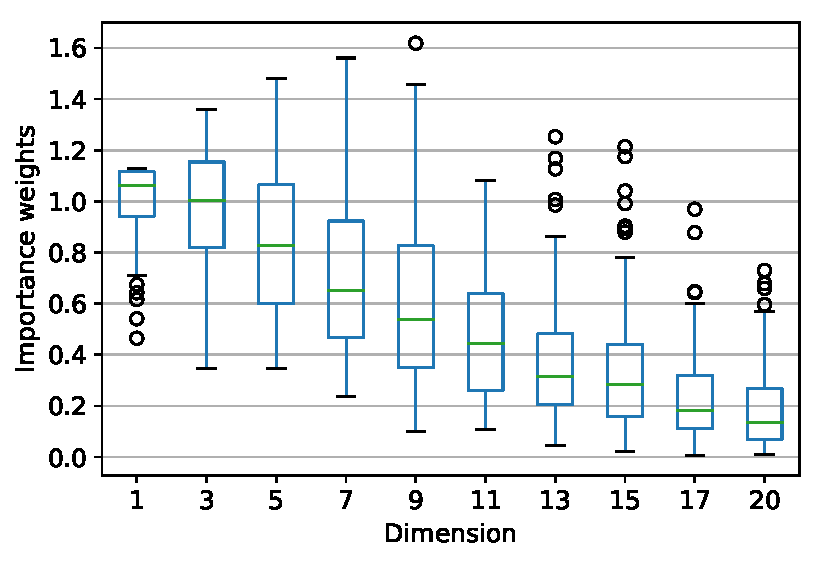
\includegraphics[height=5.1cm]{graphics/importance_mixing/importance_weights_boxplot1.pdf}
        \caption{}
        \label{fig: Theory: importance_mixing/importance_weights_boxplot1.pdf}
    \end{subfigure}
    \hfill
    \begin{subfigure}[b]{0.495\textwidth}
        \centering
        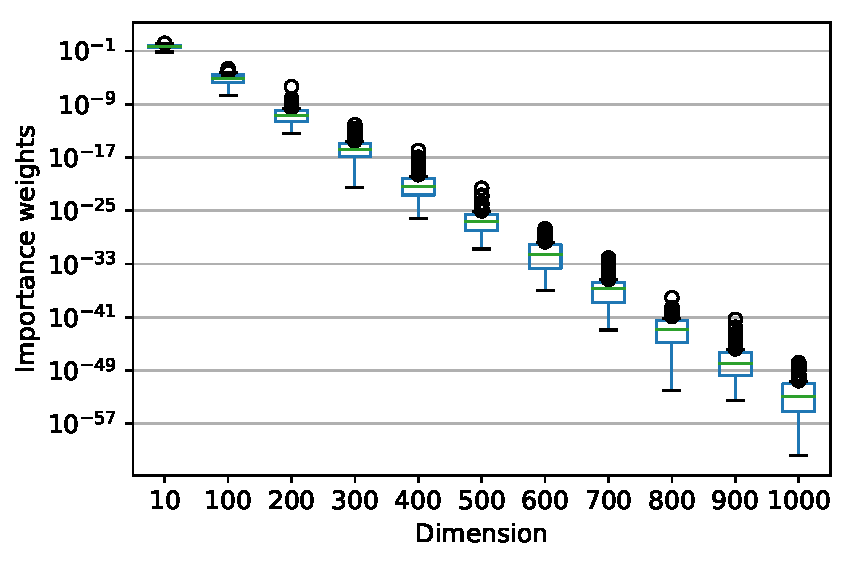
\includegraphics[height=5.1cm]{graphics/importance_mixing/importance_weights_boxplot2.pdf}
        \caption{}
        \label{fig: Theory: importance_mixing/importance_weights_boxplot.pdf2}
    \end{subfigure}
    \caption{Importance weights, such as those used in \autoref{alg: Importance mixing}, collapse for high-dimensional density functions. The figures show boxplots for the distribution of 1000 importance weights computed from samples drawn from a separable Gaussian of different dimensionalities. The importance weights are computed as $\frac{\mathcal{N}(\mub_1+\r,\text{diag}(\sigmab_1+\r)}{\mathcal{N}(\mub_2+\r,\text{diag}(\sigmab_2+\r)}$ with $\mub_1=1.1\e, \sigmab_1=0.9\e, \mub_2=1.0\e, \sigmab_2=1.0\e$ and $\r\sim\mathcal{N}(\0,0.01\e)$. \subref{fig: Theory: importance_mixing/importance_weights_boxplot1.pdf} shows dimensions one to twenty while \subref{fig: Theory: importance_mixing/importance_weights_boxplot.pdf2} shows dimensions up to 1000. (For a reference on interpretation of these boxplots, see \autoref{app: Appendix: Boxplot interpretation}.
    }
    \label{fig: Theory: importance_mixing/importance_weights_boxplot}
\end{figure}


\subsection{Adaptation sampling}\label{sec: Theory: Adaptation sampling}
Adaptation sampling is another probabilistic approach for improving \gls{VO}. As importance mixing, it relies on computation of the importance weights and as such suffers from the curse of dimensionality. Here, it is introduced nevertheless since it can potentially be used to adapt hyperparameters of the optimization problem online including the all-important learning rate. Adaptation sampling has not been used experimentally in this thesis.

First introduced in \cite{Schaul2011a} and further discussed and experimentally validated in \cite{Schaul2012}, adaptation sampling overall works by considering if a fractional change to any certain hyperparameter would have yielded a search distribution more likely to produce the best performing perturbations of the current search distribution. 

This presentation will consider the learning rate applied to the search gradient, $\eta$. Adaptation sampling is then used to determine if a hypothetical search distribution $p(\x|\thetab')$ would have been more likely to generate the best performing samples from the current distribution $p(\x|\thetab)$. The hypothetical distribution is obtained as was the current but by using a slightly larger learning rate $(1+c)\eta$ where $c>0$ is some small number. Then, importance weights are computed in the same way as for importance mixing,
\begin{equation}
    w_i=\frac{p(\x_i|\thetab')}{p(\x_i|\thetab)} \ ,
\end{equation}
for the samples $\x_i\sim p(\x|\thetab)$ for $i=1,\dots,N$. The samples are then ranked based on their fitnesses and being assigned weights with one set of ranks assigned the importance weights while another set gets unit weights,
\begin{equation}
    \begin{aligned}
        S'&\gets\cbra{\pa{w_i,\text{rank}(\x_i)}}\\
        S&\gets\cbra{\pa{1,\text{rank}(\x_i)}} \ .
    \end{aligned}
\end{equation}
The goal is then to decide if $S'$ is superior to $S$. In \cite{Schaul2011a}, a weighted version of the Mann-Whitney test is developed for this purpose. The regular Mann-Whitney test is a non-parametric test of the null hypothesis that it is equally likely that a random sample from the set $S$ will be less than or greater than a random sample from a second set $S'$ \cite{Mann1947}. 
Thus, a rejection of the null hypothesis at significance level $\rho$ is equivalent to concluding that one sample is ``larger" than the other at that significance level. If $S'$ is tested larger than $S$, the learning rate is increased by a fractional amount up to some maximal value $\eta_\text{max}$, 
\begin{equation}
    \eta\gets \min\cbra{(1+c)\eta,\eta_\text{max}}
\end{equation}
where $c$ is some small number. If $S'$ is tested smaller than $S$, the learning rate is decayed towards its initial value,
\begin{equation}
    \eta\gets(1-c)\eta+c\eta_0
\end{equation}
where $\eta_0$ is the initial value. The Mann-Whitney test and its weighted generalization are described in \autoref{app: Weighted Mann-Whitney U-test)} for convenience. The adaptation sampling procedure is summarized in \autoref{alg: Adaptation sampling}.

\begin{algorithm}[tbp!]
    \caption{Adaptation sampling \cite{Schaul2012}. \label{alg: Adaptation sampling}}
    \begin{algorithmic}[1]
        \Require{Search distribution parameters from current and previous iteration, $\thetab_t$ and $\thetab_{t-1}$. Learning rate $\eta$, initial learning rate $\eta_0$ and maximum learning rate $\eta_\text{max}$. Set of samples and associated fitnesses $\{\x_i, f(\x_i)\}$.  Increase factor/decay rate $c$ and significance level $\rho$.}
        \State Compute the hypothetical parameters $\thetab'$ using $(1+c)\eta$.
        \For{each sample $i=1,\dots,N$}
            \State Compute the importance weight 
            $$w_i=\frac{p(\x_i)|\thetab')}{p(\x_i)|\thetab)}$$
        \EndFor
        \State Compute the rank of each sample from its fitness $\{\text{rank}(\x_i)\}$
        \State Let $S$ and $S'$ be the respectively unit weighted and importance weighted sequences of ranks
        $$S\gets\{1,\text{rank}(\x_i)\}$$
        $$S'\gets\{w_i,\text{rank}(\x_i)\}$$
        \State Perform a statistical test to determine if the sequence $S'$ is superior to its $S$.
        \If{$S'$ superior} \Return $\min\cbra{(1+c)\eta, \eta_{\text{max}}}$  \Comment{Increase learning rate}
        \Else{} \Return $(1-c)\eta + c\eta_0$  \Comment{Decay learning rate towards $\eta_0$}
        \EndIf
    \end{algorithmic}
\end{algorithm}

%Although it was shown to improve performance on most of the low-dimensional common black-box optimization bench marks \cite{Schaul2012}, adaptation sampling suffers from the curse of dimensionality and importance weight collapse in the same way as importance mixing. 

% Applications of importance mixing to training of neural networks \cite{Zhao2014}, \cite{Alain2015}, \cite{Katharopoulos2017}, \cite{Katharopoulos2018}



\subsection{Safe mutation}
When perturbing network weights in order to obtain a potentially better performing network there is a significant risk that the learned transformations are broken. This can result in a model that no longer performs anywhere near the performance of the unperturbed model, at worst completely erasing all learned transformations from input to output.

In \cite{Lehman2017a}, a method for coping with this challenge was presented. The publication was part of a series of articles \cite{Lehman2017, Conti2017, Zhang2017, Such2017} that explore optimization of \glspl{NN} in the parameter space by a variant of \gls{VO} based on \cite{Salimans2017}. 
In \cite{Lehman2017a}, backpropagation is used to compute sensitivities of model output units to changes in weights. This sensitivity information can then be used to scale random perturbations of network weights so as to avoid perturbing the model in a manner that changes its output too much.

This section introduces the background of the so-called ``safe mutation" and how to appropriately compute the sensitivities and scale the sampled perturbations based on \cite{Lehman2017a}.


\subsubsection{Output divergence from weight perturbation}
Let $\y(\x,\w)=NN(\x|\w)$ denote the output $\y$ of a neural network $NN$ parameterized by $\w$ and evaluated on some input $\x$. For a mini-batch of $I$ inputs $\X=\bmat{\x_1&\dots&\x_I}$ this gives $\Y(\X,\w)=NN(\X|\w)$ with $Y_{ki}=NN(X_{:,i}|\w)_k$ equal to the $k$'th output unit's value for the $i$'th batch example. 
Now, the divergence of the output of the model that results from an additive perturbation $\epsilonb$ to its weights can be computed by 
\begin{align}
    D(\epsilonb|\w) &=
    \frac{1}{I}\sum_{k=1}^K\sum_{i=1}^I \pa{NN(\x_i|\w)_k - NN(\x_i|\w+\epsilonb)_k}^2\\
    &=
    \frac{1}{I}\sum_{k=1}^K\sum_{i=1}^I \pa{NN(\X|\w)_{ki} - NN(\X|\w+\epsilonb)_{ki}}^2 \ .
    \label{eq: Theory: Variational Optimization - Safe mutation divergence definition}
\end{align}
The divergence can thus be computed by forward propagating a mini-batch through the unperturbed and perturbed networks and summing the element-wise squared differences of their outputs, finally normalizing by the mini-batch size.




\subsubsection{Safe mutation through rescaling (SM-R)}
The simplest way to constrain the divergence of network outputs is to decompose the perturbation into a direction and a magnitude. The direction is sampled from the search distribution but is normalized to have $\norm{\epsilonb}=1$ and is then rescaled to match some predefined amount of divergence. The safe perturbation is then given by
\begin{equation}
    \epsilonb_{\text{safe}} = \alpha\epsilonb \ , 
\end{equation}
where $\alpha>0$ is the magnitude of the rescaling. This magnitude can be found using a simple line search algorithm, requiring a forward pass of the mini-batch in each of the networks and an evaluation of the divergence at every iteration. The mini-batch need not be resampled for this purpose, i.e. in reinforcement learning, no additional rollouts are required if the experiences are stored.

This rescaling approach is appealing due to its well-defined metric of ``safety" that is, it specifically chooses perturbations to give a certain amount of divergence in the network outputs. However, if a few parameters have very high sensitivities, perturbation of these may dominate the divergence and result in a rescaling factor that is very small. In turn, this leads to safe perturbations that are close to zero effectively resulting in the perturbed and unperturbed models being almost identical, $NN(\cdot|\w)\sim NN(\cdot|\w+\epsilonb_\text{safe})$. Geometrically, this is due to the direction of the perturbation being fixed while only the magnitude is rescaled.

While this rescaling approach can be applied to non-differentiable networks, gradient information of the network outputs w.r.t. the weights can be used to also change the direction of the perturbation.


\subsubsection{Safe mutation through gradients (SM-G)}
In order to scale the perturbation direction as well as the magnitude to achieve some reduction in the divergence of the network outputs, the gradient of the network outputs w.r.t. the weights can be computed. As such, safe mutation through gradients can be seen as stopping one step short in the application of the chain rule to the computational graph of the model. Instead of computing the gradient of some objective w.r.t. the network weights, the gradient is computed for the outputs themselves. For instance, in 
\begin{equation}
    \pderiv[1,1]{E}{\w} = \pderiv[1,1]{E}{\y}\pderiv[1,1]{\y}{\w}
\end{equation}
$\pderiv[1,1]{\y}{\w}$ is computed rather than $\pderiv[1,1]{E}{\w}$. In fact, $\pderiv[1,1]{\y}{\w}$ can be seen as being the Jacobian matrix describing the sensitivities of the output units to changes in the weights.

By a first order Taylor expansion, the network output at a single unit $k$ for a single example $\x_i$, $Y_{ki}=NN(\x_{i}|\w)_k$, can be seen as a function of the weight perturbation,
\begin{equation}
    Y_{ki}(\x_i,\epsilonb|\w) \approx NN(\x_{i}|\w)_k + \epsilonb\nabla_\w NN(\x_{i}|\w)_k \ .
\end{equation}
The gradient of the output w.r.t. any weight, $\nabla_\w NN(\x_{i}|\w)_k$, can thus be seen as a single point estimate of the sensitivity of that output unit to that weight. For a mini-batch of inputs, these estimates can be summed and averaged to give a better sensitivity estimate. The sensitivity of the $k$'th output unit can then be written as
\begin{equation*}
     \frac{1}{I}\sum_{i=1}^I \size{\nabla_\w NN(\X|\w)_{ki}} \ .
\end{equation*}
Here it is important to note that to compute this single unit sensitivity, each batch example must be forward propagated, have its loss evaluated, be backpropagated to compute gradients and then the gradients must be replaced by their absolute value. Although the forward pass can be batched, the \emph{absolute} gradients must be accumulated over the mini-batch when backpropagating. All modern numerical libraries for deep learning are designed to efficiently propagate batches of inputs and accumulate \emph{signed} gradients. Accumulating the absolute gradients therefore requires backpropagating each example by itself and computing the absolute gradient before backpropagating the next example. This is rather inefficient.

A much more efficient way to obtain a sensitivity estimate, is to compute an approximate per unit sensitivity by instead simply summing the signed gradients
\begin{equation*}
     \sum_{i=1}^I \nabla_\w NN(\X|\w)_{ki} \ .
\end{equation*}
According to \cite{Lehman2017a}, it empirically improves performance to not average the summed signed gradient over the batch, i.e. not divide by $I$. Summing the signed gradient introduces gradient washout while not dividing by $I$ helps keep the gradient magnitude larger, counteracting the washout.

Since the output layer generally has more than a single unit, i.e. it is a vector contrary to the usual scalar valued error function, both of these two sensitivity estimates result in a gradient for each weight, for each output unit. That is, $K$ gradients are obtained for each weight. To handle this, the gradient from each output unit is interpreted as a component of a $K$-dimensional gradient vector and the total gradient, i.e. the sensitivity, is computed as the Euclidean length of this vector. This results in two variants of the safe mutation,
\begin{align}
    \s_\text{abs} &= \sqrt{\sum_{k=1}^K \pa{\frac{1}{I}\sum_{i=1}^I\size{\nabla_\w NN(\X|\w)_{ki}}}^2}\\
    \s_\text{sum} &= \sqrt{\sum_{k=1}^K \pa{\sum_{i=1}^I\nabla_\w NN(\X|\w)_{ki}}^2} \ .
\end{align}
The absolute gradient variant is computationally much more expensive than the signed gradient variant due to the reasons discussed above. Finally, the sampled perturbation is adjusted to be safe according to the computed sensitivities,
\begin{equation}\label{eq: Theory: Safe mutation scaling}
    \epsilonb_\text{safe} = \frac{\epsilonb}{\s} \ .
\end{equation}


\subsubsection{Safe mutation through Hessian of divergence}
A slightly different approach is to consider the gradient of the divergence defined in \eqref{eq: Theory: Variational Optimization - Safe mutation divergence definition}. This allows perturbing the weights in a way that results in a certain amount of divergence, as in the rescaling approach, but here based on gradients which introduces changes to the direction as well as scaling the magnitude.

However, there is a small catch. The gradient of the divergence can be written as
\begin{align}
    \nabla_\w D(\epsilonb|\w)
    &=
    \frac{1}{I}\nabla_\w\sum_{k=1}^K\sum_{i=1}^I \pa{NN(\X|\w)_{ki} - NN(\X|\w+\epsilonb)_{ki}}^2\nonumber\\
    &=
    \frac{1}{I}\sum_{k=1}^K\sum_{i=1}^I \nabla_\w\pa{NN(\X|\w)_{ki} - NN(\X|\w+\epsilonb)_{ki}}^2\nonumber \ .
    % &=
    % \frac{2}{I}\sum_{k=1}^K\sum_{i=1}^I \pa{NN(\X|\w)_{ki} - NN(\X|\w+\epsilonb)_{ki}}\nabla_\w\pa{NN(\X|\w)_{ki} - NN(\X|\w+\epsilonb)_{ki}}\nonumber
    %&=
    %\frac{2}{I}\sum_{k=1}^K \pa{NN(\X|\w)_{:,k} - NN(\X|\w+\epsilonb)_{:,k}}\pa{\nabla_\w NN(\X|\w)_{:,k} - \nabla_\w NN(\X|\w+\epsilonb)_{:,k}}
\end{align}
% where
% \begin{equation}
%     \nabla_\w\pa{NN(\X|\w)_{ki} - NN(\X|\w+\epsilonb)_{ki}}^2 = 2\pa{NN(\X|\w)_{ki} - NN(\X|\w+\epsilonb)_{ki}}\nabla_\w\pa{NN(\X|\w)_{ki} - NN(\X|\w+\epsilonb)_{ki}}.
% \end{equation}
By the chain rule, the term in the sum becomes
\begin{equation}
    2\pa{NN(\X|\w)_{ki} - NN(\X|\w+\epsilonb)_{ki}}\nabla_\w\pa{NN(\X|\w)_{ki} - NN(\X|\w+\epsilonb)_{ki}} \ .
\end{equation}
When the gradient of the divergence is evaluated at the network's current weights $\epsilonb=0$ this term is zero and as a result, the gradient is zero. Therefore, a second order approximation must be used.

A Taylor expansion of the gradient of the divergence about the current network's weights gives a second order approximation by
\begin{align}
    \nabla_\w D(0+\epsilonb_0|\w)
    &\approx \nabla_\w D(0|\w) + \nabla_\w \bra{ \nabla_\w D(0|\w)\transpose\epsilonb_0} \nonumber\\
    &= 0 + \nabla_\w \bra{\nabla_\w D(0|\w)\transpose}\epsilonb_0 \nonumber\\
    &= \H_\w D(0|\w) \epsilonb_0
\end{align}
% which reduces to
% \begin{equation}
%     \nabla_\w D(0+\epsilonb_0|\w) \approx \H_\w D(0|\w) \epsilonb_0
% \end{equation}
since the gradient of the divergence at $\epsilonb=0$ is zero everywhere\footnote{\label{footnote: Discussion on Hessian versus vector Laplacian}There can be some confusion about the Hessian and the Laplacian. The Hessian operator can be defined as the \textit{outer} product of the gradient operator (nabla) $$\H_\w=\nabla_\w\nabla_\w\transpose$$ while the Laplacian can be defined as the \textit{inner} product of the gradient operator $$\nabla^2_\w=\nabla_\w\transpose\nabla_\w.$$ While the Hessian contains all possible second order partial derivatives, the Laplacian is the trace of the Hessian; a scalar sum of unmixed second order partial derivatives. Here, the Hessian is the operator that arises.}.
Note that the Hessian only needs to be computed as part of a matrix-vector product, $\H_\w D(0|\w) \epsilonb_0$, effectively giving the curvature of the divergence in the direction of the perturbation.

The resulting sensitivities are then computed similarly to before,
\begin{equation}
    \s_\text{SO} = \sqrt{\size{\H_\w D(0|\w)}\epsilonb}
\end{equation}
for an unscaled perturbation $\epsilonb$ which is then adjusted by $\s_\text{SO}$ according to \eqref{eq: Theory: Safe mutation scaling}.


\subsubsection{Numerical considerations}
The computation of the sensitivities derived above requires some consideration to be put into the numerical properties. Both $\s_\text{abs}$ and $\s_\text{sum}$ are computed using at least one non-normalized sum which runs the risk of numerical overflow. The implementation of the sensitivity computation used here sets any sensitivity which has overflowed to $1$. This results in that sensitivity not influencing the perturbation and the perturbation being applied as sampled. Another perhaps more sensible approach would be to set the perturbation to zero and not change the highly sensitive parameter at all. This however risks freezing that parameter indefinitely if the sensitivity does not change considerably. The sensitivity overflow problem occurs extremely rarely.

Another issue is that the numerical value of the sensitivities is somewhat arbitrary. This is most the case with the signed gradient variant which approximates the absolute gradient variant, but the problem also exists for the absolute gradient variant since the $K$ sensitivity gradients are summed at every weight. A normalization can be applied to scale the sensitivities into the range $[0,1]$
\begin{equation}
    % \hat{\s} = \frac{\s-\s_\text{min}}{\s_\text{max} - \s_\text{min}}.
    \hat{\s} = \frac{\s-\min\cbra{\s}}{\max\cbra{\s} - \min\cbra{\s}} \ .
\end{equation}
which is a natural range for a scaling applied by division.
It does however, not remove the risk of the sensitivities being zero or very close to zero which results in very large perturbations. This problem has been handled by clamping the sensitivities below by a small constant,
\begin{equation}
    \hat{\s} \leftarrow \min\cbra{\xi,\hat{\s}}
\end{equation}
Throughout this thesis, the smallest allowed sensitivity has been $\xi=10^{-2}$ which has been found to yield stable rescaling. 

Obtaining $\epsilonb_\text{safe}$ by rescaling with sensitivities in the range $[10^{-2},1]$ does not change the mean of the perturbation since it is zero but it does change the variance. In order to decouple safe mutation from the variance of the perturbation, the perturbation is finally divided by its new variance and multiplied by the wanted variance to get back the original variance in a way that corresponds to the representation and dimensionality of the search distribution. None of these considerations were described in \cite{Lehman2017a}.

%!TEX root = ../Thesis.tex



\section{Methods for variance reduction}\label{sec: Theory: Methods for variance reduction}
Monte Carlo estimators, such as the \gls{VO} gradient, are well-known to have high variance. However, many methods exist to alleviate this problem. This section considers such methods for reducing the variance of the \gls{VO} gradient estimator. First, \autoref{sec: Theory: Variance of CO estimator} derives the variance of the estimator. \autoref{sec: Theory: Antithetic sampling} derives and discusses antithetic sampling, \autoref{sec: Theory: Common random numbers} introduces the method of \gls{CRN} while \autoref{sec: Theory: Local reparameterization for variance reduction} applies a reparameterization and exploits the structure of \glspl{FNN} to obtain a lower variance estimator in a novel way.
%while stratified sampling and \gls{RSS} are presented in \autoref{sec: Theory: Stratified sampling and recurrent stratified sampling}.
%Finally, a more radical approach to variance reduction for \gls{VO} based on perturbing activations rather than weights is considered in \autoref{sec: Theory: Local reparameterization trick}.


\subsection{Variance of VO estimators}\label{sec: Theory: Variance of CO estimator}
%Another perspective on the effect of antithetic sampling can be taken by considering the variance of the \gls{VO} gradient estimator for a multivariate Gaussian search distribution. 
% Consider the variance of the \gls{VO} gradient estimator for a multivariate Gaussian search distribution. 
% This was derived for $\mub$ and $\Sigmab$ in \eqref{eq: Theory: Variational optimization multivariate gaussian gradient estimators}. Consider the gradient for $\mub$ and compute its variance as
% \begin{equation}
%     \text{Var}\left[\nabla_\mub U(\mub,\L)\right]
%     = \text{Var}\left[\frac{1}{N}\sum_{n=1}^N f(\mub+\L\epsilonb_n)(\L^{-1})\transpose\epsilonb_n\right]
% \end{equation}
% where $\epsilonb\sim\mathcal{N}(\0,\I)$ as before. The variance can be expanded in variance and covariance terms. Let $g(\epsilonb_i) = f(\mub+\L\epsilonb_i)(\L^{-1})\transpose\epsilonb_i$ for compactness. Then,

Consider the variance of the \gls{VO} gradient estimator for a general search distribution $p(\x|\thetab)$ which was derived in \eqref{eq: Theory: Variational optimization gradient estimator sampling general search distribution}. Consider the gradient for $\thetab$ and compute its variance as
\begin{align}
    \text{Var}\bra{\nabla_\thetab U(\thetab)} = \text{Var}\bra{\frac{1}{N}\sum_{n=1}^N f(\epsilonb_n) \nabla_\thetab\log p(\epsilonb_n|\thetab)}
\end{align}
where $\epsilonb$ is used in place of $\x$ to stay in the perturbation terminology. The variance can be expanded in variance and covariance terms. Let $g(\epsilonb_n) = f(\epsilonb_n) \nabla_\thetab\log p(\epsilonb_n|\thetab)$ for compactness. Then,
\begin{align} % https://en.wikipedia.org/wiki/Variance
    \text{Var}\bra{\nabla_\thetab U(\thetab)} 
    &= \text{Var}\left[\frac{1}{N}\sum_{n=1}^N g(\epsilonb_n)\right]\nonumber\\
    &= \frac{1}{N^2}\sum_{i=1}^N\sum_{j=1}^N\text{Cov}\bra{g(\epsilonb_i),g(\epsilonb_j)}\nonumber\\
    &= \frac{1}{N^2}
    \underbrace{\sum_{i=1}^N \text{Var}\bra{g(\epsilonb_i)}}_\text{diagonal} + \frac{2}{N^2}
    \underbrace{\sum_{i=1}^N\sum_{j=i+1}^N\text{Cov}\bra{g(\epsilonb_i), g(\epsilonb_j)}}_\text{off-diagonal}\label{eq: Theory: Variance of multivariate Gaussian variational optimization gradient estimator no matter the sampling}\\
    &= \frac{1}{N}\text{Var}\bra{g(\epsilonb)} + \frac{2}{N^2}\sum_{i=1}^N\sum_{j=i+1}^N\text{Cov}\bra{g(\epsilonb_i), g(\epsilonb_j)}\label{eq: Theory: Variance of multivariate Gaussian variational optimization gradient estimator regular samplng}
    %\frac{N-1}{N}\text{Cov}\bra{g(\epsilonb_i), g(\epsilonb_j)}\label{eq: Theory: Variance of multivariate Gaussian variational optimization gradient estimator}
\end{align}
when using regular sampling, $\epsilonb_i$ and $\epsilonb_j$ are \gls{IID} random variables and $\text{Cov}\bra{\epsilonb_i,\epsilonb_j}=0$ for all $i$ and $j$ where $i\ne j$. For the independence it holds more generally that $g(\epsilonb_i)$ and $h(\epsilonb_j)$ are independent for any functions $g$ and $h$. A simple argument for this is as follows: Since $\epsilonb_i$ contains no information about $\epsilonb_j$, neither will $g(\epsilonb_i)$ contain any information about $h(\epsilonb_j)$, and vice versa, regardless the functions.
% With $g(\epsilonb_i) = f(\mub+\L\epsilonb_i)(\L^{-1})\transpose\epsilonb_i$ and $h(\epsilonb_j)=g(\epsilonb_j)$,
With $g(\epsilonb_i) = f(\epsilonb_i) \nabla_\thetab\log p(\epsilonb_i|\thetab)$ and $h(\epsilonb_j)=g(\epsilonb_j)$,
\begin{equation}
     \text{Cov}\bra{g(\epsilonb_i), g(\epsilonb_j)} = 0 \ ,\quad \forall\;i,j \text{ with } i\ne j \ .
\end{equation}
The variance of the gradient estimate then reduces to include only the diagonal of the covariance matrix, i.e. the variances
%\begin{equation}
%    \text{Var}\left[\nabla_\mub U(\mub,\L)\right] = \frac{1}{N^2}\sum_{i=1}^N \text{Var}\bra{g(\epsilonb_i)}.
%\end{equation}
%Since $\epsilonb_i$ are \gls{IID} for all $i$, this simplifies to
\begin{equation}
    \text{Var}\bra{\nabla_\thetab U(\thetab)} = \frac{1}{N} \text{Var}\bra{g(\epsilonb)} \ .\label{eq: Theory: Variance of regular Monte Carlo VO gradient estimator for arbitrary search distribution}
\end{equation}
Thus, the variance of the \gls{VO} gradient estimator is $\mathcal{O}(1/N)$ where $N$ is the number of perturbations. This result and the following results for antithetic sampling hold when considering a single batch example. The case of mini-batches with additive objective functions are considered in \autoref{sec: Theory: Local reparameterization for variance reduction}. 
This result holds regardless of the choice of search distribution as long as the samples are \gls{IID}.


\subsection{Antithetic sampling}\label{sec: Theory: Antithetic sampling}
A simple but powerful method for variance reduction in stochastic estimation is that of antithetic sampling. This method was successfully applied for stochastic estimation of gradients using an isotropic Gaussian search distribution with fixed variance in \cite{Salimans2017} although no theoretical argument for its efficiency was provided.

For every sampled path $\{\epsilon_1,\epsilon_2,\dots,\epsilon_n\}$, antithetic sampling simply consists of also taking the so-called antithetic or mirrored path.
%defined by $\{-\epsilon_1,-\epsilon_2,\dots,-\epsilon_n\}$. 
This effectively doubles the number of samples obtained by sampling which may be beneficial in it self in the case where sampling is expensive.

Considering stochastic gradient estimation using a search distribution, the antithetic samples form a vector in the search space that points in the exact opposite direction of the original samples. Intuitively speaking, in the case that the original samples proved to give lower function values, the antithetic sampling then probes the opposite path and if it gives higher function values, the variance is reduced due to negative covariance. 

% This intuition can be shown mathematically. 
% Consider the task of estimating the derivative of a univariate objective function using the \gls{VO} approach resulting in an estimator like that in \eqref{eq: Theory: Taylor: Univariate gradient estimator from standard Gaussian} or \eqref{eq: Theory: Variational optimization univariate gaussian gradient estimators} repeated here for convenience
% \begin{equation*}
%     U'(\mu) = \frac{1}{\sigma}\text{E}\bra{f(\mu + \sigma\epsilon)\epsilon}
% \end{equation*}

% Now generate two samples $f(\mu + \sigma\epsilon_1)\epsilon_1$ and $f(\mu + \sigma\epsilon_2)\epsilon_2$ each resulting in their own estimate $\hat{U}_1'(\mu)$ and $\hat{U}_2'(\mu)$. An unbiased total estimate is then simply
% \begin{equation}
%     \hat{U}'(\mu) = \frac{\hat{U}_1'(\mu) + \hat{U}_2'(\mu)}{2}
% \end{equation}
% Notice however that the variance of this estimator is given by
% \begin{equation}
%     \text{Var}\bra{\hat{U}'(\mu)} = \frac{1}{4}\pa{\text{Var}\bra{\hat{U}_1'(\mu)} + \text{Var}\bra{\hat{U}_2'(\mu)} + 2\text{Cov}\bra{\hat{U}_1'(\mu), \hat{U}_2'(\mu)}}
% \end{equation}
% In the case that the sampled paths $\hat{U}_1'(\mu)$ and $\hat{U}_2'(\mu)$ have negative covariance, this reduces the variance compared to uncorrelated sample paths which would have $\text{Cov}\bra{\hat{U}_1'(\mu),\hat{U}_2'(\mu)}=0$. 

For the \gls{IID} sampling, the covariance was shown to be zero. However, a negative covariance will result in a reduction of the variance compared to regular \gls{IID} sampling. If $\epsilonb_i$ and $\epsilonb_j$ are chosen to not all be independent, the covariance becomes nonzero.  
One way to correlate the perturbations is to choose the mirrored perturbation given by $\tilde{\epsilonb}_i=c-\epsilonb_i$, for every $\epsilonb_i$, where $c$ is the center of symmetry of the search distribution. This is the method of antithetic sampling. 
When the search distribution is symmetric around zero, as can for instance be made the case for any Gaussian perturbation by the reparameterization trick, $c=0$ and $\tilde{\epsilonb}_i=-\epsilonb_i$ to give
\begin{equation}
    \text{Cov}\bra{\epsilonb_i,\tilde{\epsilonb}_i} = \text{Cov}\bra{\epsilonb_i,-\epsilonb_i} = -\text{Var}\bra{\epsilonb_i} \ .
%    &= \text{E}\bra{-\epsilonb_i\epsilonb_i\transpose} - \text{E}\bra{\epsilonb_i}\text{E}\bra{-\epsilonb_i}\nonumber\\
%    &= -\text{E}\bra{\epsilonb_i\epsilonb_i\transpose}\nonumber\\
%    &= -\text{Var}\bra{\epsilonb_i}
\end{equation}
%To not increase the total number of samples one should take for instance $\epsilonb_{i+1} = -\epsilonb_i$, in effect.
%It should be noted that the indices $i$ and $j$ are not as in the covariance matrix being summed in \eqref{eq: Theory: Variance of multivariate Gaussian variational optimization gradient estimator} but merely represent antithetic pairs.
To compute the total covariance between perturbations, $\text{Cov}\bra{g(\epsilonb_i), g(\epsilonb_j)}\;\forall i,j$, consider first the covariance between any antithetic pair, $\text{Cov}\bra{g(\epsilonb), g(\tilde{\epsilonb})}$. This is most easily done by decomposing $g(\cdot)$ in its odd and even components as follows. An even function $e$ satisfies $e(x)=e(-x)$ and an odd function $o$ satisfies $o(x)=-o(-x)$. It follows that any function, here $g$, can be decomposed into even and odd parts by writing
\begin{subequations}
    \begin{align}
        g_e(\epsilonb) &= \frac{g(\epsilonb)+g(-\epsilonb)}{2}\label{eq: Theory: Antithetic sampling even and odd function decomposition definition a}\\
        g_o(\epsilonb) &= \frac{g(\epsilonb)-g(-\epsilonb)}{2}\label{eq: Theory: Antithetic sampling even and odd function decomposition definition b}\\
        g(\epsilonb) &= g_e(\epsilonb) + g_o(\epsilonb)\label{eq: Theory: Antithetic sampling even and odd function decomposition definition c}
    \end{align}
\end{subequations}
where $g_e$ denotes the even component and $g_o$ denotes the odd. The even and odd components are orthogonal in the sense that $\int g_\text{e}(\epsilonb)g_\text{o}(\epsilonb)\,\text{d}\epsilonb = 0$. The covariance can then be calculated by the following manipulations.
\begin{align}
    \text{Cov}\bra{g(\epsilonb),g(-\epsilonb)}
    &= \text{Cov}\bra{g_e(\epsilonb) + g_o(\epsilonb),g_e(-\epsilonb) + g_o(-\epsilonb)}\nonumber\\
    %&= \text{Cov}\bra{g_e(\epsilonb), g_e(-\epsilonb)} + \text{Cov}\bra{g_o(\epsilonb), g_o(-\epsilonb)} + \text{Cov}\bra{g_e(\epsilonb), g_o(-\epsilonb)} + \text{Cov}\bra{g_o(\epsilonb), g_e(-\epsilonb)} \nonumber\\
    %&= \text{Cov}\bra{g_e(\epsilonb), g_e(\epsilonb)} -     \text{Cov}\bra{g_o(\epsilonb), g_o(\epsilonb)} - \text{Cov}\bra{g_e(\epsilonb), g_o(\epsilonb)} + \text{Cov}\bra{g_o(\epsilonb), g_e(\epsilonb)} \nonumber\\
    &= \text{Var}\bra{g_e(\epsilonb)} - \text{Var}\bra{g_o(\epsilonb)} \ .
\end{align}
% \begin{align}
%     \text{Cov}\bra{g(\epsilonb),g(-\epsilonb)}
%     &= \text{Cov}\bra{g_e(\epsilonb) + g_o(\epsilonb),g_e(-\epsilonb) + g_o(-\epsilonb)}\nonumber\\
%     &= 
%     \begin{aligned}[t]
%         &\text{Cov}\bra{g_e(\epsilonb), g_e(-\epsilonb)} + 
%         \text{Cov}\bra{g_o(\epsilonb), g_o(-\epsilonb)} \\
%         & \quad + \text{Cov}\bra{g_e(\epsilonb), g_o(-\epsilonb)} + 
%         \text{Cov}\bra{g_o(\epsilonb), g_e(-\epsilonb)}
%     \end{aligned}
%     \nonumber\\
%     &= 
%     \begin{aligned}[t]
%         & \text{Cov}\bra{g_e(\epsilonb), g_e(\epsilonb)} - 
%         \text{Cov}\bra{g_o(\epsilonb), g_o(\epsilonb)} \\
%         & \quad - \text{Cov}\bra{g_e(\epsilonb), g_o(\epsilonb)} + 
%         \text{Cov}\bra{g_o(\epsilonb), g_e(\epsilonb)}
%     \end{aligned}
%     \nonumber\\
%     &= \text{Var}\bra{g_e(\epsilonb)} - \text{Var}\bra{g_o(\epsilonb)} \ .
% \end{align}
Evidently, the covariance is negative if the odd component has larger variance than the even component which results in lower total variance compared to \gls{IID} sampling.  
Since the covariances are only nonzero for the antithetic pairs, the covariance matrix will be block diagonal with $2\times2$ blocks, assuming that the mirrored sample is introduced as $\epsilonb_{i+1} = -\epsilonb_i$ where $i\in[0,2,4,\dots,N/2]$ and $N$ is even. There will then be $N/2$ nonzero covariances in the lower triangular matrix such that \eqref{eq: Theory: Variance of multivariate Gaussian variational optimization gradient estimator regular samplng} reduces to
\begin{align}
    \text{Var}\bra{\nabla_\thetab U(\thetab)_a}
    &= \frac{1}{N}\text{Var}\bra{g(\epsilonb)} + \frac{1}{N}\text{Cov}\bra{g(\epsilonb), g(-\epsilonb)}
\end{align}
where $\nabla_\thetab U(\thetab)_a$ denotes the antithetic \gls{VO} gradient estimate.
In fact, if $g_e(\epsilonb)=0$ such that $g(\epsilonb)=g_o(\epsilonb)$ is purely odd, then $\text{Cov}\bra{g_o(\epsilonb),g_o(-\epsilonb)} = - \text{Var}\bra{g_o(\epsilonb)}$ and $\text{Var}\bra{\nabla_\thetab U(\thetab)_a}=0$. 
If instead $g(\epsilonb)=g_e(\epsilonb)$, then $\text{Var}\bra{\nabla_\thetab U(\thetab)_a}=2\text{Var}\bra{g_e(\epsilonb)}$. 
\begin{equation}
    \text{Var}\bra{\nabla_\thetab U(\thetab)_a} = 
    \begin{cases}
        0 & \text{if } g(\epsilonb)=g_o(\epsilonb)\\
        2\text{Var}\bra{g_e(\epsilonb)} & \text{if } g(\epsilonb)=g_e(\epsilonb)
    \end{cases}\label{eq: Theory: Antithetic sampling best and worst cases}
\end{equation}
These two extremes are respectively the best and worst case scenarios for antithetic sampling. At best, the variance is reduced to zero and the gradient is exact after evaluating only at one pair of perturbations. At worst, the variance of the gradient is doubled.

%\begin{equation}
%    \text{Var}\left[\nabla_\mub U(\mub,\L)\right]
%    &= \frac{1}{2}\text{Var}\bra{g_o(\epsilonb_i)} - \frac{1}{2} \text{Var}\bra{g_o(\epsilonb)} = 0.
%\end{equation}
%If $g$ is purely even then
%\begin{equation}
%    \text{Var}\left[\nabla_\mub U(\mub,\L)\right]
%    &= \frac{1}{N}\text{Var}\bra{g_o(\epsilonb_i)} - \frac{N-1}{N} \text{Var}\bra{g_o(\epsilonb)} = 0.
%\end{equation}

Instead of writing the regular estimator and taking $\epsilonb_{i+1}=-\epsilonb_i$, alternatively one can write the antithetic \gls{VO} gradient estimate directly
\begin{equation}\label{eq: Antithetic sampling: direct antitethetic estimate}
    \nabla_\thetab U(\thetab)_a = \frac{1}{N}\sum_{n=1}^{N/2} g(\epsilonb_n) + g(-\epsilonb_n)
\end{equation}
where $N$ again must be an even integer. This can be written in terms of the even component of the function by \eqref{eq: Theory: Antithetic sampling even and odd function decomposition definition a} 
\begin{equation}
    \nabla_\thetab U(\thetab)_a = \frac{2}{N}\sum_{n=1}^{N/2} g_e(\epsilonb_n) \ .
\end{equation}
Now, the variance of the antithetic estimator becomes
\begin{align}
    \text{Var}\bra{\nabla_\thetab U(\thetab)_a}
    &= \frac{4}{N^2}\text{Var}\bra{\sum_{n=1}^{N/2} g_e(\epsilonb_n)}\nonumber\\
    %&= \frac{4}{N^2}\sum_{i=1}^{N/2}\sum_{j=1}^{N/2}\text{Cov}\bra{g_e(\epsilonb_i),g_e(\epsilonb_j)}\nonumber\\
    %&= \frac{4}{N^2}\sum_{i=1}^{N/2} \text{Var}\bra{g_e(\epsilonb_i)} + \frac{8}{N^2}\sum_{i=1}^{N/2}\sum_{j=i+1}^{N/2}\text{Cov}\bra{g_e(\epsilonb_i), g_e(\epsilonb_j)}\nonumber\\
    &= \frac{4}{N^2}\sum_{n=1}^{N/2} \text{Var}\bra{g_e(\epsilonb_n)}\nonumber\\
    %&= \frac{4N/2}{N^2}\text{Var}\bra{g_e(\epsilonb)}\nonumber\\
    &= \frac{2}{N}\text{Var}\bra{g_e(\epsilonb)}
\end{align}
since the covariance is zero in this formulation. From \eqref{eq: Theory: Variance of regular Monte Carlo VO gradient estimator for arbitrary search distribution}, the variance of the ordinary \gls{VO} gradient estimator can similarly be split into even and odd function components which gives
\begin{equation}
    \text{Var}\bra{\nabla_\thetab U(\thetab)_a} = \frac{1}{N}\pa{\text{Var}\bra{g_e(\epsilonb)} + \text{Var}\bra{g_o(\epsilonb)}}
\end{equation}
since $\text{Cov}\bra{g_e(\epsilonb_n), g_o(\epsilonb_n)}=0$ due to orthogonality. Clearly then, antithetic sampling trades in the variance of the odd component for the variance of the even component. In summary one can write
\begin{equation}
    \bmat{\text{Var}\bra{\nabla_\thetab U(\thetab)}\\\text{Var}\bra{\nabla_\thetab U(\thetab)_a}} = \frac{1}{N}\bmat{1&1\\2&0}\bmat{\text{Var}\bra{g_e(\epsilonb)}\\\text{Var}\bra{g_o(\epsilonb)}}
\end{equation}
which is a generalization of \eqref{eq: Theory: Antithetic sampling best and worst cases}. Evidently, there is a potentially large variance reduction to gain from using antithetic sampling on a function that is primarily odd or at least has most of its variance in the odd component. 

By expanding $g(\epsilonb)$ in a Taylor series and plugging it into \eqref{eq: Antithetic sampling: direct antitethetic estimate} there is another perspective to antithetic sampling to be noted. Consider the univariate case where $\epsilon$ is scalar. The argument holds for the multivariate case as well. The Taylor series can be written as
\begin{equation}
    g(\epsilon) = \sum_{i=0}^\infty \frac{g^\pa{i}(0)}{i!}\epsilon^i \ .
\end{equation}
With $\tilde{\epsilon}=-\epsilon$ then
\begin{align}
    g(\epsilon) + g(\tilde{\epsilon})
    &= g(\epsilon) + g(-\epsilon)\\
    &= \sum_{i=0}^\infty \frac{g^\pa{i}(0)}{i!}\epsilon^i + \sum_{i=0}^\infty \frac{g^\pa{i}(0)}{i!}\pa{-\epsilon}^i\\
    &= \sum_{i=0}^\infty \frac{g^\pa{i}(0)}{i!}\epsilon^i + \pa{\sum_{i=0,2,\dots}^\infty \frac{g^\pa{i}(0)}{i!}\epsilon^i - \sum_{i=1,3,\dots}^\infty \frac{g^\pa{i}(0)}{i!}\epsilon^i}\\
    &= \sum_{i=0,2,\dots}^\infty \frac{g^\pa{i}(0)}{i!}\epsilon^i + \sum_{i=0,2,\dots}^\infty \frac{g^\pa{i}(0)}{i!}\epsilon^i\\
    &= 2\sum_{i=0,2,\dots}^\infty \frac{g^\pa{i}(0)}{i!}\epsilon^i \ .
\end{align}
Clearly then, the antithetic sampling serves to cancel out odd derivatives of the Taylor series of $g$ while doubling the contribution of the even derivatives. 

In \gls{VO}, the function $g$ is composed by the objective function $f$ multiplied by the perturbation $\epsilonb$. In the reinforcement learning setting, the objective is expected to exhibit some degree of anti-symmetry while it is unlikely to be purely odd. For instance, in highly symmetric mazes walking in the $x$ direction can be equivalent to walking in the $-x$ direction but generally it is not.
This thesis will not attempt to analyze how anti-symmetry holds through the multiplication by $\epsilonb$ and perturbation of the \gls{NN} parameters by $\epsilonb$, however, it seems there is reason to conjecture that antithetic sampling may reduce the gradient estimate variance.

An additional note can be made about the subspace spanned by the \gls{VO} perturbations when using antithetic sampling. Without antithetic sampling, $N$ random perturbations are likely to span an $N$ dimensional subspace of the $d$ dimensional search space. When using antithetic sampling, half of these perturbations are replaced by the negative of an already existing perturbation. As such, the antithetic perturbations are linearly dependent on the existing perturbations. Consequently, the subspace will be maximally $N/2$ dimensional for a population of $N$ perturbations.

% \todo[inline]{Is $\epsilonb f(\x+\epsilonb)$ generally more odd than even?
% The product of two even functions is an even function.
% The product of two odd functions is an even function.
% The product of an even function and an odd function is an odd function.
% Derive this relation using Taylor approximation of $g(\dot)$}

\iffalse
The variance then becomes
\begin{align}
    \text{Var}\bra{\nabla_\mub U(\mub,\L)}
    &= \text{Var}\bra{\frac{1}{N}\sum_{n=1}^{N/2} g(\epsilonb_n) + g(\tilde{\epsilonb}_n)}\nonumber\\
    &= \frac{\L^{-1}}{N^2}\text{Var}\bra{\sum_{n=1}^{N/2} g(\epsilonb_n) + g(\tilde{\epsilonb}_n)}\nonumber\\
    &= \frac{N/2}{N^2}\text{Var}\bra{g(\epsilonb) + g(\tilde{\epsilonb})}\nonumber\\
    &= \frac{1}{2N}\pa{\text{Var}\bra{g(\epsilonb)} + \text{Var}\bra{g(\tilde{\epsilonb})} + 2\text{Cov}\bra{g(\epsilonb),g(\tilde{\epsilonb}}}\nonumber\\
    &= \frac{1}{N}\pa{\text{Var}\bra{g(\epsilonb)} + 
    \text{Cov}\bra{g(\epsilonb),g(\tilde{\epsilonb}}}\nonumber
\end{align}


Additionally, for $g(\epsilonb_i) = f(\mub+\L\epsilonb_i)\epsilonb_i$, if $g$ is odd, then $g(-\epsilonb_i)=-g(\epsilonb_i)$ and
\begin{equation}
    \text{Cov}\bra{g(\epsilonb_i),g(-\epsilonb_i)} = \text{Cov}\bra{g(\epsilonb_i),-g(\epsilonb_i)} = -\text{Var}\bra{g(\epsilonb_i)} \ .
\end{equation}
Obviously it cannot be assumed that $g$ is an entirely odd function. However, any function can be decomposed into even and odd parts which are orthogonal. That is, one can write

$\text{Cov}\bra{f(\mub+\L\epsilonb_i)\epsilonb_i, f(\mub+\L\epsilonb_j)\epsilonb_j}$
% \nabla_\mub U(\mub,\L) &= (\L^{-1})\transpose\text{E}\bra{f(\mub+\L\epsilonb)\epsilonb} \approx \frac{\L^{-1}}{N}\sum_{n=1}^N f(\mub+\L\epsilonb)\epsilonb


\begin{align} % https://en.wikipedia.org/wiki/Variance
    \text{Var}\left[f'(x)\right]
    &= \text{Var}\left[\frac{1}{N\sigma}\sum_{n=1}^N f(x+\sigma\hat{\epsilon}_n)\hat{\epsilon}_n\right]\nonumber\\
    &= \frac{1}{N^2\sigma^2}\sum_{i=1}^N\sum_{j=1}^N\text{Cov}\bra{f(x+\sigma\hat{\epsilon_i}}\hat{\epsilon_i}, \bra{f(x+\sigma\hat{\epsilon_i}}\hat{\epsilon_i}\\
    &= \frac{1}{N^2\sigma^2}\pa{\sum_{i=1}^N \text{Var}\left[f(x+\sigma\hat{\epsilon}_i)\hat{\epsilon}_i\right] + 2\sum_{i=1}^N\sum_{j=i+1}^N\text{Cov}\bra{f(x+\sigma\hat{\epsilon_j}}\hat{\epsilon_j}, \bra{f(x+\sigma\hat{\epsilon_i}}\hat{\epsilon_i}}
\end{align}


Consider the task of estimating
\begin{equation}
    \theta = \text{E}\bra{Y}
\end{equation}
from samples of $Y=h(X)$. Now generate two samples $Y_1$ and $Y_2$ each resulting in their own estimate $\hat{\theta_1}$ and $\hat{\theta_2}$. An unbiased total estimate is then simply
\begin{equation}
    \hat{\theta} = \frac{\hat{\theta_1} + \hat{\theta_2}}{2}
\end{equation}
Notice however that the variance of this estimator is given by
\begin{equation}
    \text{Var}\bra{\hat{\theta}} = \frac{\text{Var}\bra{Y_1} + \text{Var}\bra{Y_2} + 2\text{Cov}\bra{Y_1,Y_2}}{4} \ .
\end{equation}
In the case that the sampled paths $Y_1$ and $Y_2$ have negative covariance, this reduces the variance compared to uncorrelated sample paths which would have $\text{E}\bra{\text{Cov}\bra{Y_1,Y_2}}=0$. That is, the variance reduction originates from the assumption that negative covariance between the sampled paths results in negative covariance between the function values.
\fi










\subsection{Common random numbers}\label{sec: Theory: Common random numbers}
The method of \gls{CRN} is usually applied when comparing two or more stochastic simulations of some system for a some different sets of hyperparameters. The simulations are then made such that any stochastic elements of the systems share the same seed for all the simulations. That is, the stochastic elements in each simulation are identical, at least initially. For instance, if random noise is added in an otherwise deterministic simulation of a system, the sequence of random numbers that represent the noise is the same for all the simulations. The simulations may still differ due to the different hyperparameter settings.  The reduced amount of randomness in turn reduces variance \cite{Glasserman2003}.

In the application of \gls{VO} to supervised learning, the method of \gls{CRN} translates to evaluating each of the perturbations on the same mini-batch of training examples. Specifically, in classification, if the batch over-represents some class which the model is particularly bad at correctly classifying, any perturbation that outperforms the others has a good chance of improving on classifying that class. If the batches were different, some models may be evaluated too harshly due to being handed a difficult batch compared to the batches given to other perturbations.

In the \gls{RL} setting, it corresponds to evaluating the perturbations on environments which have been seeded such that they have the same initial condition. In \gls{RL}, the episodes that follow may be quite different despite the shared initial state due to the different policies represented by the perturbed networks.
 




\subsection{Local reparameterization}\label{sec: Theory: Local reparameterization for variance reduction}
The local reparameterization method \cite{Kingma2015a} was presented as a means of reducing the variance of the \gls{SGVB} method \cite{Kingma2013} which seeks to perform efficient approximate inference and learning in directed graphical models in the fully Bayesian setting. Here, the approach is applied to reduce the variance of the \gls{VO} estimator. This section describes an untried idea that should be subject to further analysis and experimental validation.

\subsubsection{An alternative Monte Carlo estimator for the upper bound}
The local reparameterization is useful in situations where the objective $f(\x)$ is composed of a sum of individual terms, typically averaged. Then
\begin{equation}
    f(\x)=\frac{1}{\size{\mathcal{B}}}\sum_{b\in\mathcal{B}}f_b(\x)
\end{equation}
where $f_i(\x)$ denotes the objective evaluated at the network with parameters $\x$ on the $b$'th batch example. 
This is the case for error functions in supervised learning \eqref{eq: Neural networks: Error as a sum over individual terms}. 
In such a case, the \gls{VO} upper bound can be rewritten as
\begin{equation}
    U(\thetab) = \text{E}\bra{f(\x)}_{p(\x|\thetab)} = \frac{1}{\size{\mathcal{B}}}\sum_{b\in\mathcal{B}}\text{E}\bra{f_b(\x)}_{p(\x|\thetab)} \ .
\end{equation}
An unbiased Monte Carlo estimator for $U(\thetab)$ is then % Although the gradient of $U(\thetab)$ is
\begin{equation}\label{eq: Theory: Local reparameterization: U estimator, reused weights for each example}
    U(\thetab) \approx \frac{1}{N\size{\mathcal{B}}}\sum_{n=1}^N\sum_{b\in\mathcal{B}}f_b(\x_n)
\end{equation}
which is effectively the same result as previously seen for the gradient. However, rather than using the same weights for all examples in a batch, one can now sample new weights for each example. This results in the following alternative unbiased Monte Carlo estimator.
\begin{equation}\label{eq: Theory: Local reparameterization: U estimator, new weights for each example}
    \tilde{U}(\thetab) \approx \frac{1}{N\size{\mathcal{B}}}\sum_{n=1}^N\sum_{b\in\mathcal{B}}f_b(\x_{bn}) \ .
\end{equation}

\subsubsection{Variance of the upper bound estimators}
The variance of the estimator in \eqref{eq: Theory: Local reparameterization: U estimator, reused weights for each example} is
\begin{align}
    \text{Var}\bra{U(\thetab)}
    &= \frac{1}{N^2\size{\mathcal{B}}^2}\sum_{n,n'=1}^N\sum_{b,b'\in\mathcal{B}}\text{Cov}\bra{f_b(\x_n),f_{b'}(\x_{n'})}\nonumber\\
    &= \frac{1}{N^2\size{\mathcal{B}}^2}\sum_{n=1}^N\sum_{b\in\mathcal{B}}\text{Var}\bra{f_b(\x_n)} + \frac{1}{N^2\size{\mathcal{B}}^2}\sum_{\substack{n,n'=1\\n\ne n'}}^N\sum_{\substack{b,b'\in\mathcal{B}\\b\ne b'}}\text{Cov}\bra{f_b(\x_n),f_{b'}(\x_{n'})}\nonumber\\
    &= \frac{1}{N\size{\mathcal{B}}^2}\sum_{b\in\mathcal{B}}\text{Var}\bra{f_b(\x)} + \frac{N-1}{N\size{\mathcal{B}}^2}\sum_{\substack{b,b'\in\mathcal{B}\\b\ne b'}}\text{Cov}\bra{f_b(\x),f_{b'}(\x)}\nonumber\\
    &= \frac{1}{N\size{\mathcal{B}}}\text{Var}\bra{f_b(\x)} + \frac{N-1}{N}\frac{\size{\mathcal{B}}-1}{\size{\mathcal{B}}}\text{Cov}\bra{f_b(\x),f_{b'}(\x)}
\end{align}
where it is used that the within-batch covariance is the same on average, as for the perturbations.
This result may at first seem to contradict \eqref{eq: Theory: Variance of regular Monte Carlo VO gradient estimator for arbitrary search distribution} but in fact does not. 
In \eqref{eq: Theory: Variance of regular Monte Carlo VO gradient estimator for arbitrary search distribution}, only a single batch-example was considered while here, an entire mini-batch is studied including the potentially non-zero between-batch covariance. It should be noted that the variance scales as $\mathcal{O}\pa{1/N\size{\mathcal{B}}}$ while the covariance scales as $\mathcal{O}(1)$ for large enough $N$ and $\size{\mathcal{B}}$ and as such effectively lower bounds $\text{Var}\bra{U(\thetab)}$.

By the same manipulations, the variance of the estimator in \eqref{eq: Theory: Local reparameterization: U estimator, new weights for each example} that samples new parameters for each batch example is
\begin{equation*}
    \text{Var}\bra{\tilde{U}(\thetab)}
    = \frac{1}{N\size{\mathcal{B}}}\text{Var}\bra{f_b(\x_{b})} + \frac{N-1}{N}\frac{\size{\mathcal{B}}-1}{\size{\mathcal{B}}} \text{Cov}\bra{f_b(\x_{b}),f_{b'}(\x_{b'})}
\end{equation*}
but here it is noted that the covariance term can be rewritten
\begin{align}
    \text{Var}\bra{\tilde{U}(\thetab)}
    &= \frac{1}{N\size{\mathcal{B}}}\text{Var}\bra{f_b(\x_{b})} + \frac{N-1}{N}\frac{\size{\mathcal{B}}-1}{\size{\mathcal{B}}}\text{E}\bra{\pa{f_b(\x_{b})-U_b}\pa{f_{b'}(\x_{b'})-U_{b'}}}_{p(\x_b|\thetab),p(\x_{b'}|\thetab)}\nonumber\\
    &= \frac{1}{N\size{\mathcal{B}}}\text{Var}\bra{f_b(\x_{b})} + \frac{N-1}{N}\frac{\size{\mathcal{B}}-1}{\size{\mathcal{B}}}\pa{\text{E}\bra{f_b(\x_{b})}_{p(\x_b|\thetab)}-U_b}\pa{\text{E}\bra{f_{b'}(\x_{b'})}_{p(\x_{b'}|\thetab)}-U_{b'}}\nonumber\\
    &= \frac{1}{N\size{\mathcal{B}}}\text{Var}\bra{f_b(\x_{b})}
\end{align}
where $U_b = \text{E}\bra{f_{b}(\x_{b})}_{p(\x_b|\thetab)}$. The covariance term is zero in the alternative estimator that samples new parameters for the model for each batch example.


\subsubsection{Propagation of a distribution over activations}
The derivation made to give \eqref{eq: Theory: Variational optimization gradient estimator sampling general search distribution} is followed again to obtain the Monte Carlo estimator for the gradient of the alternative estimator, 
\begin{equation}
    \nabla_\thetab \tilde{U}(\thetab) \approx \frac{1}{N\size{\mathcal{B}}}\sum_{n=1}^N\sum_{b\in\mathcal{B}}f_b(\x_{bn})\nabla_\thetab\log p(\x_{bn}|\thetab) \ ,
\end{equation}
where $x_{b,n}\sim p(\x_{b,n}|\thetab)$. From a computational point of view this estimator is not very efficient and especially not for modern deep learning software which is optimized to evaluate a single network on $\size{\mathcal{B}}$ training examples. The advantage of the formulation is that the variance of the estimator is reduced from $\mathcal{O}(1)$ to $\mathcal{O}(1/N\size{\mathcal{B}})$ because each term is evaluated on an independent realization of the parameters \cite{Kingma2015a}. 


To achieve computational efficiency, it is exploited that \gls{FNN} models depend upon the weights and biases only through the activations, $\Z^\bra{l}=\W^\bra{l}\A^\bra{l-1}$ where $\A^\bra{l}=\varphi\pa{\Z^\bra{l}}$, as discussed in \autoref{chp: Neural networks}. In elementwise notation this becomes $Z^\bra{l}_{ib}=\sum_jW^\bra{l}_{ij}A^\bra{l-1}_{jb}$, where $Z^\bra{l}_{ib}$ is the $i$'th element in the $l$'th layer activation of the $b$'th batch example.
The following will consider the isotropic Gaussian search distribution $p(\W|\thetab)=\mathcal{N}\pa{\W|\mub,\sigma^2\I}$ with $\thetab=\cbra{\mub, \sigma^2}$ and sample by reparameterization, $\W=\mub+\sigma\epsilonb, \epsilonb\sim\mathcal{N}(\0,\I)$.
The distribution of the activations can be inferred from the distribution of the weights drawn for each training example. Taking $\mub$ and $\sigma$ to be matrices of same shape as $\W$, this distribution is
\begin{equation}\label{eq: Theory: Variance reduction: Inferred distribution of activations for local reparameterization trick}
    q\pa{Z_{ib}^\bra{l} \;\middle|\; \A^\bra{l-1},\thetab} = \mathcal{N}\left(Z_{ib}^\bra{l} \;\middle|\; \sum_j \mu_{ij}^\bra{l} A_{jb}^\bra{l-1}, \sum_j \sigma^{\bra{l}^2}_{ij} A^{\bra{l-1}^2}_{jb}\right) = \mathcal{N}\left(Z_{ib}^\bra{l} \;\middle|\; m_{ib}^\bra{l}, v_{ib}^\bra{l}\right)
\end{equation}
where $m_{ib}$ and $v_{ib}$ are respectively the mean and variance of the Gaussian activation distribution. 
By letting $\Z_{bn}$ denote the stacked vector of activations of all layers of the $b$'th batch example and $n$'th perturbation\footnote{Strictly speaking, here $\Z$ is a third order tensor with elements $Z_{ibn}$ denoting the $i$'th element of the $b$'th batch example activation for the $n$'th perturbation. Activation vectors of all layers are then stacked into a single dimension, $i$.} and similarly for $\A_{bn}$ then
\begin{equation}
\label{eq:gradient2}
    \nabla_\thetab \tilde{U}(\theta) \approx \frac{1}{N\size{\mathcal{B}}} \sum_{n=1}^N\sum_{b\in\mathcal{B}} f_b(\Z_{bn}) \nabla_\thetab
    \log q(\Z_{bn}|\A_{bn},\thetab) \ ,
\end{equation}
where $Z_{ibn} = m_{ib} + \sqrt{v_{ib}}\,\xi_{ibn}$, with $\xi_{ibn}\sim\mathcal{N}(0,1)$ and $f(\Z)$ is the error function from above now written in terms of the activations.
With this, the Monte Carlo estimates for the derivatives are
\begin{equation}\label{eq: Theory: Local reparameterization: Gradient of upper bound isotropic/full Gaussian}
    \begin{aligned}
        \pderiv{\tilde{U}(\thetab)}{\mu_{ij}^\bra{l}} &\approx \frac{1}{N\size{\mathcal{B}}} \sum_{n=1}^N\sum_ {b\in\mathcal{B}} f_b(\Z_{bn}) \frac{\xi_{ibn}}{\sqrt{v_{ib}^\bra{l}}} A_{jb}^\bra{l-1} \\
        \pderiv{\tilde{U}(\thetab)}{\sigma_{ij}^{\bra{l}^2}} &\approx \frac{1}{N\size{\mathcal{B}}} \sum_{n=1}^N\sum_ {b\in\mathcal{B}} f_b(\Z_{bn}) \frac{\xi_{ibn}^2 - 1}{2 v_{ib}^\bra{l}} A_{jb}^{\bra{l-1}^2} \ .
    \end{aligned}
\end{equation}

The complexity of a forward pass with this new approach is $\mathcal{O}\pa{N\size{\mathcal{B}}\size{\Z}}$ where $\size{\Z}$ is the number of activations/units in the network. The batch can be efficiently forward propagated in a single pass as described in \autoref{chp: Neural networks}. For comparison, the original approach has a complexity of $\mathcal{O}\pa{N\size{\W}}$ while a naive implementation of local reparameterization has a complexity of $\mathcal{O}\pa{N\size{\mathcal{B}}\size{\W}}$ and additionally requires a forward pass for each batch example which is less efficient than the new approach. The local reparameterization thus improves computational efficiency by sampling activations rather than weights.

With $\A^\bra{0} = \X$, the forward pass in an \gls{FNN} is %$Z^\bra{l}_{ib} = m^{(l)}_{ib} + \sqrt{v^{(l)}_{ib}} \xi^{(l)}_{ib}$ or 
\begin{subequations}
    \begin{align}
        \m^\bra{l} & = \mub^\bra{l} \A^\bra{l-1} \\
        \v^\bra{l} & = \left( \sigmab^\bra{l} \A^\bra{l-1}\right)^2 \\
        \Z^\bra{l} & = \m^\bra{l} + \sqrt{\v^\bra{l}} \odot \xib^\bra{l}\\
        \A^\bra{l} &= \varphi\pa{\Z^\bra{l}} \ ,
    \end{align}
\end{subequations}
when vectorized appropriately\footnote{The activation mean and variance $\m^\bra{l}$ and $\v^\bra{l}$ both have dimensions of $\A^\bra{l}$. The unperturbed network is parameterized by $\mub^\bra{l}$ which has dimensions of $\W^\bra{l}$; as has the associated perturbation variance $\sigmab^2$.}. This effectively forward propagates a distribution over activations without realizing the perturbed weights explicitly and instead perturbs the activations.


\subsubsection{Alternative gradient estimator variance}
In addition to improving computational efficiency, the local reparameterization also reduces the variance of the gradient estimator. Comparing the estimators in \eqref{eq: Theory: Local reparameterization: Gradient of upper bound isotropic/full Gaussian} with the ones derived earlier for the isotropic Gaussian in \eqref{eq: Theory: Variational optimization multivariate isotropic gaussian gradient estimators} it is evident that they are similar but the alternative version derived here perturbs in the activation space rather than the weight space. 
As was discussed in \autoref{sec: Theory: Taylor expansion interpretation of derivatives as covariances}, estimating the gradient has an interpretation as estimating the covariance between the objective and the perturbations. Since the alternative estimator based on the local reparameterization perturbs the activation space its search space has much fewer dimensions. These and their respective perturbations will then individually have much higher correlation with the objective and so the covariance, and hence the gradient, will be easier to accurately estimate \cite{Kingma2015a}.


\subsubsection{Relation to batch normalization}
Batch normalization was introduced in \autoref{chp: Neural networks}. The local reparameterization derived here is not directly affected by the normalization applied to the activations by batch normalization. Likewise, batch normalization is not affected by the forward propagation of a distribution over activations and can simply be applied to these activations as usual.

In fact, it seems that batch normalization can benefit from the local reparameterization by exploiting the already computed mean and variance of the activations. That is, \eqref{eq: Neural networks: Batch normalization: Mean} and \eqref{eq: Neural networks: Batch normalization: Variance} can be replaced with
\begin{equation}
    \overline{\m}  = \text{E}\left[\m\right]_{p(\Z|\A)} = \frac{1}{\size{\mathcal{B}}} \sum_{b\in\mathcal{B}} \m_{b}
\end{equation}
and
\begin{equation}
    \overline{\v}  = \text{E}\left[\v\right]_{p(\Z|\A)} = \frac{1}{\size{\mathcal{B}}} \sum_{b\in\mathcal{B}} \left( \v_b + \pa{\m_b - \overline{\m}}^2 \right) +\mathcal{O}(\size{\mathcal{B}}^{-1})
\end{equation}
respectively, for each layer. This results in slightly reduced computation required since the running mean variance are no longer required although a mean is still computed over the activations. 


\subsubsection{Remarks on application to convolutional neural networks}
In a \gls{CNN}, the same kernel is applied across the entire input which results in the activations of a \gls{CNN} layer being highly correlated. The covariance between input pixels $i$ and $i'$ will be $\sum_j \sigma^2_j A_{jb} A_{j'b}$ where $j$ are the pixels in the input corresponding to pixel $i$ in the feature map.
A single sample of the feature map activations thus requires diagonalizing a covariance matrix of size $\pa{\#\text{pixels}\times\#\text{pixels}}$. 
This is rather inefficient even if structure in the matrix can be exploited.
Therefore, it seems better to stick with the original approach for convolutional layers of the network.




% \subsection{Stratified sampling and recurrent stratified sampling}\label{sec: Theory: Stratified sampling and recurrent stratified sampling}
% \todo[inline]{(Write about stratified sampling)}
% \gls{BSS}

% \gls{RSS}

% % http://www.aip.de/groups/soe/local/numres/bookcpdf/c7-8.pdf

% % https://pdfs.semanticscholar.org/f260/6f334bd4865b105005b887478003ce9bd3e2.pdf

% % http://users-phys.au.dk/tberg/numeric/project/bo.pdf

% \cite{Press2007}



% %\section{Curiosity driven optimization}
% %\todo[inline]{Examine curiosity driven optimization using a GP to fit to the fitnesses and perturbations}
% %Using \glspl{GP} to fit to the samples and fitness values and compute expected fitness.
% %\cite{Schaul2011a}



%!TEX root = ../Thesis.tex

\chapter{Experimental work}\label{chp: Experimental results}
% Qoute ...
\chapterquote{It is shown that many particular choices among possible neurophysiological assumptions are equivalent, in the sense that for every net behaving under one assumption, there exists another net which behaves under the other and gives the same results, although perhaps not in the same time.}{McCulloch, W.S. and Pitts, W. H. (1943) \cite{McCulloch1943}}

%!TEX root = ../Thesis.tex

\section{Introduction}
In addition to the theoretical work presented in the preceding chapters, this thesis has spent some effort on implementing and experimenting with the different methods, algorithms and augmentations. The algorithms have been implemented in Python using parts of the PyTorch deep learning library.
Brief explanations and references to full code repositories are given in \autoref{app: implementations of algorithms}. The experiments were run on the \gls{HPC} cluster at DTU. This section presents the results of the experimental work. 

\autoref{sec: Experimental work: Benchmarking} presents the problems used for the benchmarking and while the different \gls{NN} architectures used are described in \autoref{sec: Experimental work: Neural network architectures}. 
The general computational complexity and scaling properties of the \gls{VO} algorithm are examined for both a supervised problem and a reinforcement learning problem in \autoref{sec: Experimental work: Computational scaling}.
\autoref{sec: Experimental work: Effects of common model and algorithm augmentations} examines the influence of the model augmentations of batch normalization and dropout along with safe mutation.
In \autoref{sec: Theory: Methods for variance reduction}, the different methods for reducing the variance of the gradient are examined- This includes gradient momentum in \ref{sec: Experimental work: Effect of momentum} and antithetic sampling in \ref{sec: Experimental work: Antithetic sampling}.
Finally, the effect of adapting the variance using different Gaussian search distributions is evaluated in \autoref{sec: Experimental work: Effect of adapting the variance}.

It should be noted that the number of hyperparameters combined with variations on the \gls{VO} algorithm gives a large number of potential experiments to conduct. This thesis has only performed a small subset of all the possible experiments. The chosen experiments were selected based on what had the highest potential to show improvement to the algorithm.

%!TEX root = ../Thesis.tex

\section{Benchmark problems}\label{sec: Experimental work: Benchmarking}
\subsection{Supervised learning benchmark}
Within the supervised learning setting, the classical problem of handwritten digit recognition based on the \gls{MNIST} dataset \cite{LeCun1998} was chosen. This is a small and relatively simple data set that has allowed for rapid prototyping and aided in algorithm development, historically and in this thesis. Even though it has recently received criticism for being too simple, it remains one of the most widely used benchmarks within deep learning \cite{Xiao2017}. The training data consists of 60.000 greyscale images of handwritten digits between 0 and 9 and the associated label. Each image has $28\times28$ pixels and represents a single digit. The test data consists of 10.000 images and associated labels.
In this thesis, no data augmentation has been applied to the data set. Examples from the \gls{MNIST} dataset can be seen in \autoref{fig: mnist-examples/MNIST-10x10-sorted.pdf}.
\begin{figure}[tbp!]
    \centering
    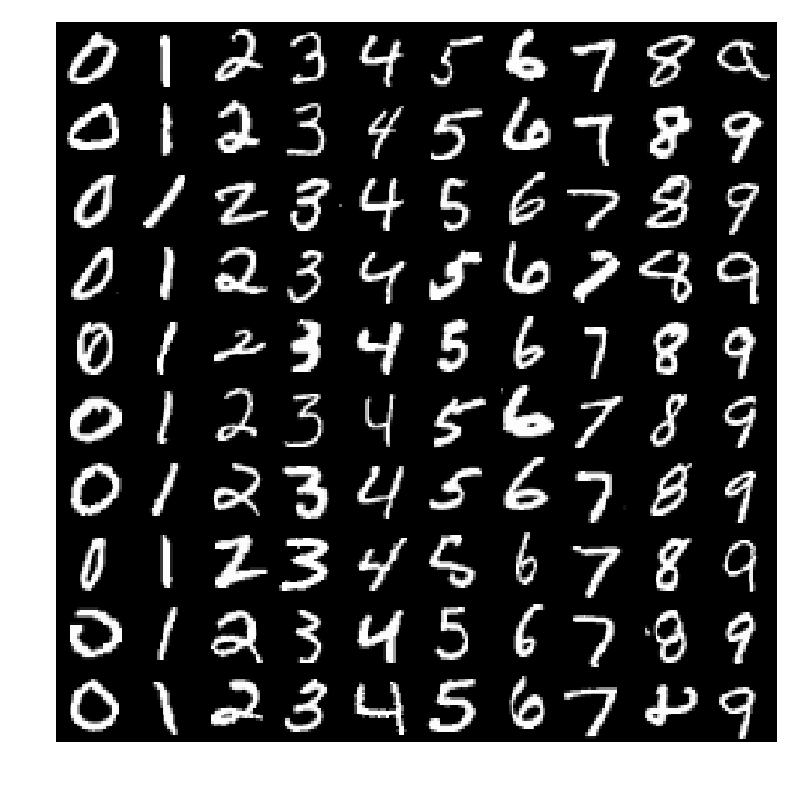
\includegraphics[width=0.60\textwidth]{graphics/mnist-examples/MNIST-10x10-sorted.pdf}
    \caption{
        Examples from the \gls{MNIST} dataset sorted by target values from 0 on the left and 9 on the right. As is well-known, a few examples from the dataset are very hard to correctly classify, note for example the bottom most 8 and the top most 9.
    }
    \label{fig: mnist-examples/MNIST-10x10-sorted.pdf}
\end{figure}

To the author's best knowledge, the currently best performing non-ensemble \gls{NN} model on \gls{MNIST} is the deep \gls{FNN} using DropConnect \cite{Wan2013, Hasanpour2016} which achieved $99.79\%$ classification accuracy also exploiting extreme data augmentation. An accuracy of $99.76\%$ was achieved in \cite{Chang2015} which uses a max-out network in network \cite{Lin2013} model with no data augmentation. Using backpropagation and the network to be used for \gls{MNIST} in this thesis (introduced in \autoref{sec: Experimental work: Neural network architectures (MNIST)} and shown in \autoref{lst: Network models: MNIST with batch normalization}) the best achievable accuracy is about $99.1\%$ using \gls{SGD} with momentum training for 20 epochs. With the Adam algorithm, accuracy can reach $99.2\%$ for 20 epochs.


\subsection{Reinforcement learning benchmarks}
Within the reinforcement learning setting, focus has been primarily on two environments from the OpenAI Gym toolkit \cite{Brockman2016}. The first environment is the Atari-2600 game of Freeway\footnote{\url{http://en.wikipedia.org/wiki/Freeway_(video_game)}, \url{http://gym.openai.com/envs/Freeway-v0/}} in which the agent controls a chicken that must be brought to pass a busy ten lane highway by moving either up or down. If hit by a car, the chicken is pushed either slightly back or moved to the starting position. A reward of $1$ is given for each successful passage and the total score is the number of passages within a time slot of $2$ minutes and $16$ seconds. In \cite{Salimans2017}, using a the fixed variance \gls{ES} similar to \gls{VO}, a score of $31$ was achieved when averaged over 10 re-runs with the DQN network of \cite{Mnih2016} encoding a deterministic policy. This network is also used for \gls{RL} in this thesis

The second \gls{RL} environment is the Atari game of Seaquest\footnote{\url{http://en.wikipedia.org/wiki/Seaquest_(video_game)}, \url{http://gym.openai.com/envs/Seaquest-v0/}}. Here, the agent controls a submarine which must fend off enemies using torpedoes while rescuing divers by moving to their location. The submarine's oxygen supply is limited and the agent must occasionally bring it to the surface to refill and to receive points from rescued divers. The submarine can move in four directions and fire torpedoes. Seaquest is considered harder than Freeway due to the larger action space and more complicated objective. In \cite{Salimans2017}, a score of $1390.0$ was achieved in the same way as for Freeway.

In this thesis, \gls{VO} is used to optimize a policy which maps from the environment's observation space to its action space. The policy is parameterized by a \gls{NN} model, in this case also called a policy network \cite{Silver2014}. The policy is deterministic in that the most probable action, as computed by the policy network, is always taken. Due to computational limitations, the number of experiments made in the reinforcement setting is fewer than in the supervised setting.

In general, hyperparameter optimization has been performed manually and heuristically. Ideally, random hyperparameter search \cite{Bergstra2012a} would have been employed to find optimal hyperparameters but was not due to limited computational resources.


\subsection{Preprocessing of MNIST}
Although no data augmentation is applied to the \gls{MNIST} dataset, the data is normalized before being input to the \gls{NN}. That is, for each digit image, the average pixel value is computed along with the variance and these are aggregated to a mean and variance for the full dataset. For \gls{MNIST}, this could be done in a single computation since the entire data set fits in memory. However, since larger datasets were also tried out, the computation was implemented in an online manner according to the algorithm proposed by \cite{Welford1962}. 

The algorithm consists of updating the mean as usual and the variance through online updates to the squared sample distance from the mean. For the mean
\begin{equation}
    \bar{x}_n = \bar{x}_{n-1} + \frac{x_n-\bar{x}_{n-1}}{n} \ .
\end{equation}
% \begin{align*}
%     \bar{x}_n
%     &= \frac{1}{n}\sum_{i=1}^n x_i\\
%     %&= \frac{1}{n}\pa{\sum_{i=1}^{n-1} x_i + x_n}\\
%     &= \frac{n-1}{n}\frac{1}{n-1}\sum_{i=1}^{n-1} x_i + \frac{1}{n}x_n\\
%     &= \frac{n-1}{n}\bar{x}_{n-1} + \frac{1}{n}x_n\\
%     &= \bar{x}_{n-1} + \frac{x_n-\bar{x}_{n-1}}{n} \ .
% \end{align*}
%which can be written as
%\begin{equation}
%    \bar{x}_n = \bar{x}_{n-1} + \frac{x_n-\bar{x}_{n-1}}{n} \ .
%\end{equation}
Likewise, the update for the variance is
\begin{align*}
    s^2_n
    &= \frac{(n-2)}{(n-1)} s^2_{n-1} + \frac{(x_n - \bar{x}_{n-1})^2}{n} \ , \quad n>1 \ .
\end{align*}
This online update of the variance is prone to numerical instability which is avoided by updating the squared sample distance from the mean
\begin{equation*}
    M_{2,n} = M_{2,n-1} + (x_n - \bar{x}_{n})^2 %(x_n - \bar{x}_{n-1})(x_n - \bar{x}_{n})
\end{equation*}
and then computing 
\begin{equation*}
    s_n^2 = \frac{M_{2,n}}{n-1} \ .
\end{equation*}
These formulas have been generalized to the case of multiple examples being added at each online update \cite{Chan1979}. Here, this is needed to avoid looping over the $28\times28=784$ pixels of each image. Let $A$ and $B$ denote two samples with $n_A$ and $n_B$ examples respectively and a mean, variance and squared sample distance from the mean denoted by $\bar{x}_A$, $\bar{x}_B$, $s^2_A$, $s^2_B$, $M_{2,A}$, $M_{2,B}$, respectively. The update formulas for the aggregated sample $X$ are then
\begin{align*}
    \delta &= \bar{x}_B - \bar{x}_A\\
    \bar{x}_X &= \frac{n_A}{n_X}\bar{x}_A + \frac{n_B}{n_X}\bar{x}_B\\
    M_{2,X} &= M_{2,A} + M_{2,B} + \delta^2\frac{n_A n_B}{n_X}\\
    s_X^2 &= \frac{M_{2,X}}{n_X-1}
\end{align*}
where $n_X = n_A + n_B$.

The computed mean and standard deviation for the \gls{MNIST} dataset were then used to normalize each input pixel $x_i$ as
\begin{equation*}
    \hat{x}_i = \frac{x_i-\bar{x}}{s} \ .
\end{equation*}


\subsection{Preprocessing of Atari environments} \label{sec: Experimental section: Preprocessing of Atari environments}
Atari environments are preprocessed in the same way as in \cite{Mnih2015}. A frame from an Atari game is a $210\times160\times3$ pixels RGB image. Due to the limited number of sprites an Atari 2600 was able to display at once, some objects in games occur only in even frames while others occur only in odd frames \cite{Mnih2015}. To remove this flickering, a single frame is encoded as the maximum value of each pixel of the most recent frame and the previous frame. The frame is then converted to greyscale and resized to $84\times84$ using a pixel area relation which gives moiré-free results, is fast and yields good results for image downsampling \cite{OpenCVDevelopmentTeam2014}. This reduces the dimensionality of the frame by more than a factor of ten from $210\times160\times3=100800$ pixels to $84\times84=7056$ pixels. The input given to the \gls{NN} model is the four most recent frames seen such that the input dimension is $4\times84\times84$. This gives the model directional information about movement in the images without the use of recurrent units.

\begin{figure}[tbp!]
    \begin{subfigure}[b]{0.32\textwidth}
        \centering
        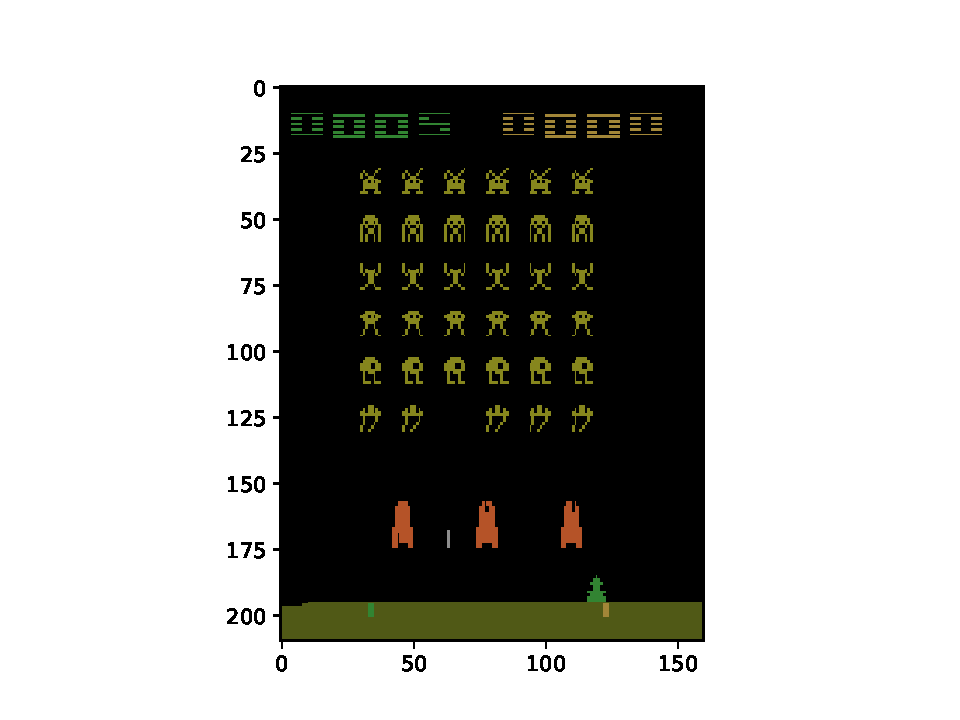
\includegraphics[height=5.8cm]{graphics/atari-pre-processing/1-spaceinvaders-original-cropped.pdf}
        \caption{}
        \label{fig: Experimental work: atari-pre-processing-1-spaceinvaders-original}
    \end{subfigure}
    \hfill
    \begin{subfigure}[b]{0.32\textwidth}
        \centering
        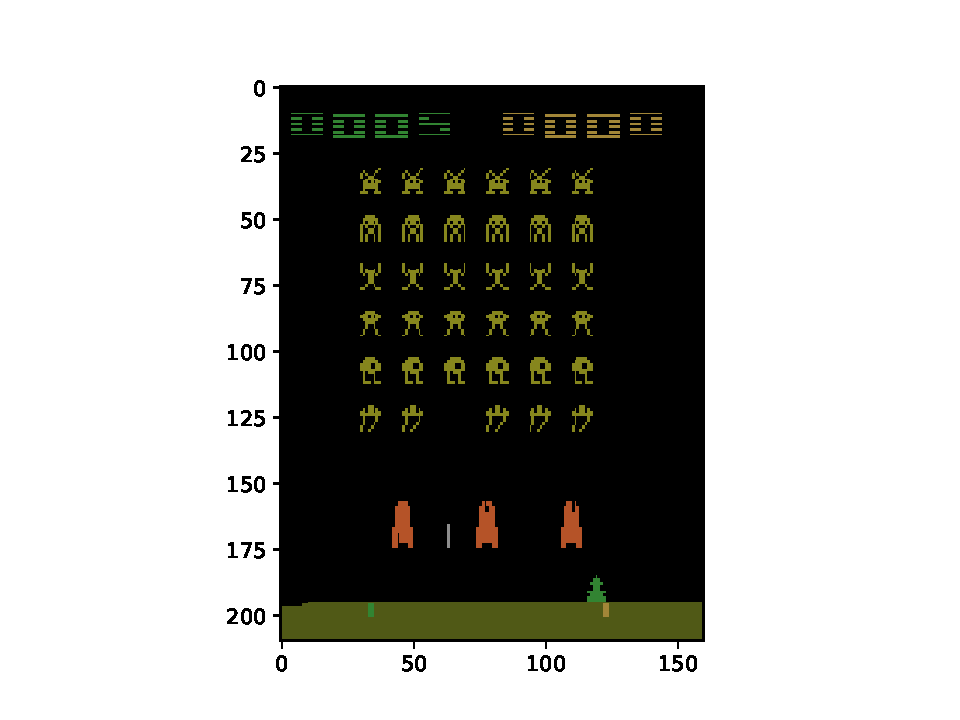
\includegraphics[height=5.8cm]{graphics/atari-pre-processing/2-spaceinvaders-flicker-cropped.pdf}
        \caption{}
    \label{fig: Experimental work: atari-pre-processing-2-spaceinvaders-flicker}
    \end{subfigure}
    \hfill
    \begin{subfigure}[b]{0.32\textwidth}
        \centering
        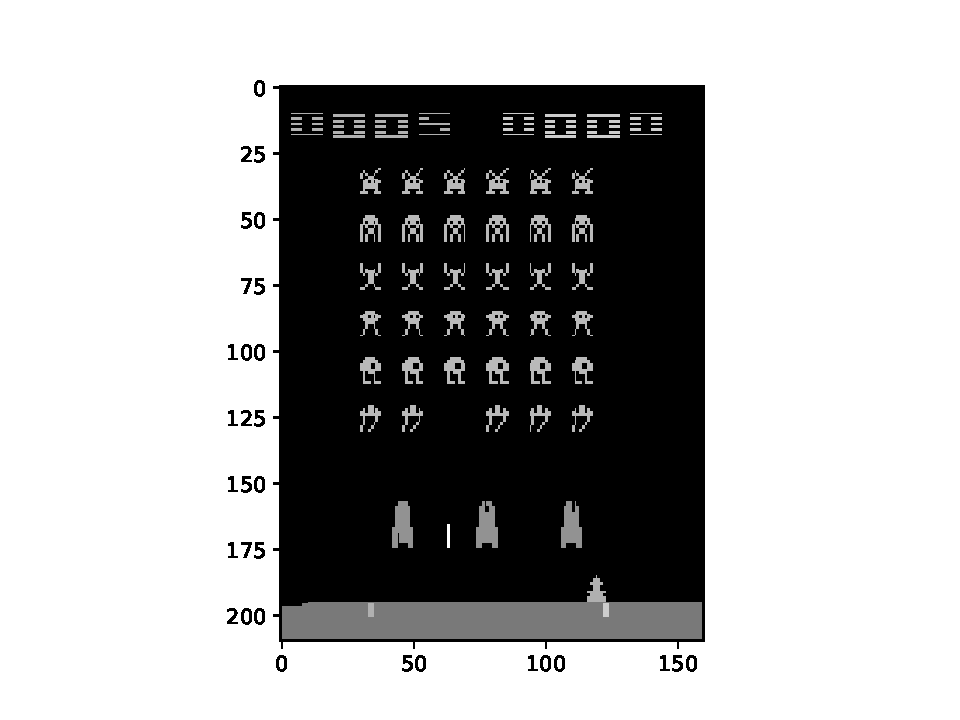
\includegraphics[height=5.8cm]{graphics/atari-pre-processing/3-spaceinvaders-grey-cropped.pdf}
        \caption{}
        \label{fig: Experimental work: atari-pre-processing-3-spaceinvaders-grey}
    \end{subfigure}
    \centering
    \begin{subfigure}[b]{0.40\textwidth}
        \centering
        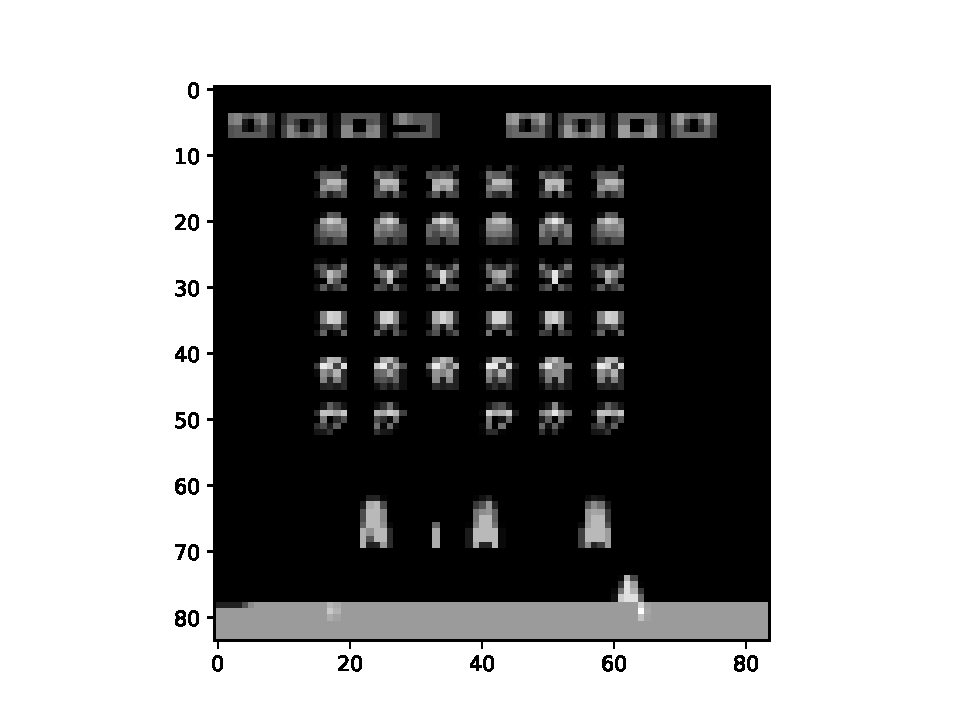
\includegraphics[height=5.8cm]{graphics/atari-pre-processing/4-spaceinvaders-resized-cropped.pdf}
        \caption{}
        \label{fig: Experimental work: atari-pre-processing-4-spaceinvaders-resized}
    \end{subfigure}
    \caption{\subref{fig: Experimental work: atari-pre-processing-1-spaceinvaders-original} Original frame from Space Invaders. \subref{fig: Experimental work: atari-pre-processing-2-spaceinvaders-flicker} Flicker removed by setting pixels to their maximal value over previous four frames. Notice the elongated beam. \subref{fig: Experimental work: atari-pre-processing-3-spaceinvaders-grey} Converted to greyscale. \subref{fig: Experimental work: atari-pre-processing-4-spaceinvaders-resized} Resized to $84\times84$.}
    \label{fig: Experimental work: atari-pre-processing}
\end{figure}

An illustration of the results of this preprocessing can be seen for the game of Space Invaders in \autoref{fig: Experimental work: atari-pre-processing}. Note that the fired beam is longer in \subref{fig: Experimental work: atari-pre-processing-2-spaceinvaders-flicker} compared to \subref{fig: Experimental work: atari-pre-processing-1-spaceinvaders-original}. This is a side effect of combining successive images by pixel maximum which slightly elongates moving objects.

%!TEX root = ../Thesis.tex

\section{Network architectures}\label{sec: Experimental work: Neural network architectures}
%This section describes the \gls{NN} model architectures used for the benchmark problems. Detailed model summaries can be found in \autoref{app: models}.


\subsection{Architecture for MNIST}\label{sec: Experimental work: Neural network architectures (MNIST)}
For the \gls{MNIST} problem, a simple \gls{CNN} with 22.000 parameters has been used. Overall, the network has two convolutional layers each followed by batch normalization, max pooling and a ReLU nonlinearity. Fully connected layers follow; the first with batch normalization and ReLU nonlinearity; the second with log-softmax nonlinearity.

In more detail, the first layer is a convolution layer with $10$ $5\times5$ kernels and $10$ biases and is applied to the single greyscale channel of the input images. This layer is followed by a batch normalization layer with a mean and standard deviation for each of the 10 kernels and a learned affine transformation. A max pooling layer with $2\times2$ kernel and no padding is then applied. Finally, a ReLU nonlinearity is applied. The second convolution layer has $20$ kernels but is otherwise identical to the first also followed by batch normalization, max pooling and ReLU nonlinearity. The following fully connected layer has the $320$ outputs of the preceding convolution layer as input and has $50$ outputs followed by batch normalization and ReLU nonlinearity. The output layer of the model is fully connected with $50$ inputs and $10$ outputs, one for each digit. A log-softmax nonlinearity is applied to the output units and combined with the \gls{NLL} loss. \autoref{lst: Network models: MNIST with batch normalization} contains a summary of this network.


\subsection{Architecture for Atari environments}\label{sec: Experimental work: Neural network architectures (RL}
The network architecture used for learning policies for the Atari environments is the same as the one used by \cite{Mnih2015, Silver2016}. In short, the network is a \gls{CNN} with three convolutional layers followed by two fully connected layers totalling 1.685.667 parameters, most of them in the first linear layer.

In more detail, the first convolutional layer has $32$ $8\times8$ kernels, $32$ biases and is applied to each of the four most recent frames, each of which is treated as a channel. This layer has a stride of $4$ and is followed by a ReLU nonlinearity. The second convolutional layer has $64$ $4\times4$ kernels, $64$ biases and is applied to each of the $32$ $20\times20$ outputs of the previous layer. It has a stride of $2$ and is also followed by a ReLU nonlinearity. The third and final convolutional has $64$ $3\times3$ kernels, $64$ biases and is applied to each of the $64$ $9\times9$ outputs of the previous layer. It has a stride of $1$ and is followed by a ReLU nonlinearity. A fully connected layer with $64\times7\times7=3136$ inputs, $512$ outputs and a ReLU nonlinearity connects the flattened output of the final convolutional layer with the output layer. The output layer is fully connected and followed by a log-softmax nonlinearity with its number of outputs defined by the specific Atari environment. For the Freeway environment it is $3$ while for Seaquest it is $18$. \autoref{lst: Network models: DQN network for Atari environments} contains a summary of this network.



%One for each problem type:
%MNIST
%CIFAR-10 
%- Data set\cite{Krizhevsky2009}
%- Model \cite{Hertel2015}
%Atari



%!TEX root = ../Thesis.tex

\section{Computational scaling}\label{sec: Experimental work: Computational scaling}
%This section presents the parallel scaling capabilities of the \gls{VO} method as applied to both supervised and reinforcement learning problems.

\subsection{Scaling in supervised learning}
\begin{figure}[tbp!]
    \begin{subfigure}[b]{0.517\textwidth}
        \centering
        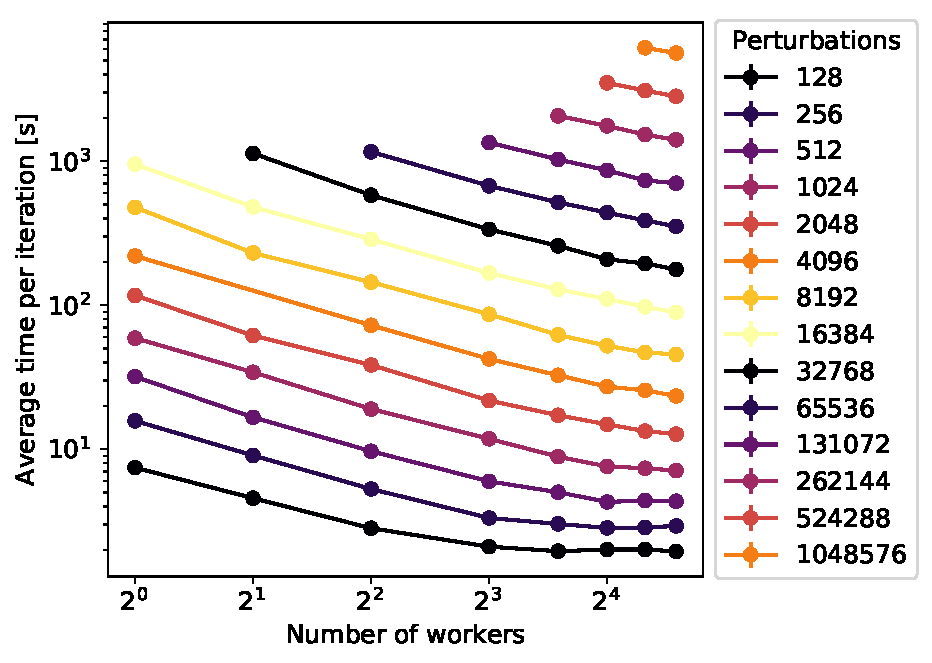
\includegraphics[height=5.6cm]{graphics/E005-sca-analysis/E005-scaling-02.pdf}
        \caption{}
        \label{fig: Theory: E005-scaling-supervised-02}
    \end{subfigure}
    \hfill
    \begin{subfigure}[b]{0.473\textwidth}
        \centering
        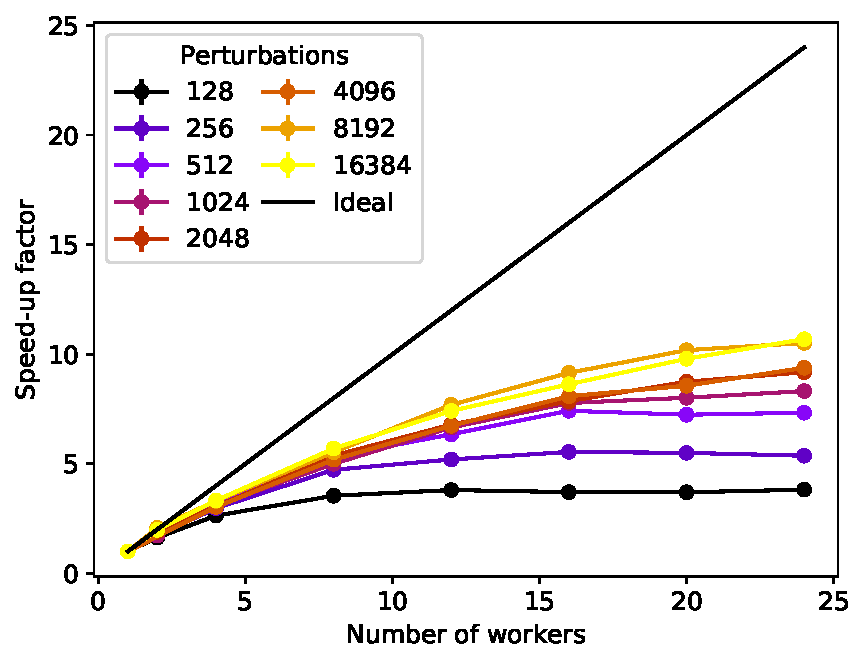
\includegraphics[height=5.6cm]{graphics/E005-sca-analysis/E005-scaling-04.pdf}
        \caption{}
        \label{fig: Theory: E005-scaling-supervised-04}
    \end{subfigure}
    \caption{
        Computational scaling in the supervised setting for different numbers of \glspl{CPU} and perturbations. Each observation is the average over 100 iterations with associated standard deviation (too small to discern).
        \subref{fig: Theory: E005-scaling-supervised-02} The average time spent per iteration in seconds.
        \subref{fig: Theory: E005-scaling-supervised-04} The observed speedup.
    }
    \label{fig: Theory: E005-scaling-supervised}
\end{figure}
This section presents the computational scaling of the \gls{VO} method used to train the \gls{MNIST} architecture described above when using a several \glspl{CPU} and varying the number of perturbations. 
Each setting of number of perturbations was run for 100 iterations and evaluated on a mini-batch of 200 images.
%Each perturbation was evaluated on a mini-batch of 200 images and each iteration of the algorithm evaluates some number of perturbations and was timed. 
The mean time and variance were computed from the 100 iterations run for each combination of number of \glspl{CPU} and perturbations.

\autoref{fig: Theory: E005-scaling-supervised-02} shows the average time spent per iteration as a function of the number of \glspl{CPU} used for various numbers of perturbations. The scaling can be seen to be fairly good for a high enough number of perturbations. Since the evaluation of every perturbation is a single forward pass through the network, the fitness evaluation is quite fast and slower function evaluations would give better scaling. \autoref{fig: Theory: E005-scaling-supervised-04} shows the measured speedup as a function of the number \glspl{CPU} for different perturbations. %This is a popular plot for presenting parallel performance and illustrates Amdahl's law \cite{Amdahl1967}. 
It is evident that speedup quickly drops off from the ideal although an order of magnitude speedup is observed for 24 \glspl{CPU}.

Obviously, \gls{VO} is an inefficient choice for optimizing differentiable \glspl{NN} in the supervised setting. Backpropagation excels at this task while also allowing for efficient batch parallelization on \glspl{GPU}.
%This points out the inefficiency of applying \gls{VO} to cases with relatively low cost fitness evaluations. Higher parallel
%Furthermore, this forward pass can be significantly sped up by using \glspl{GPU}.

\subsection{Scaling on a reinforcement learning problem}
\begin{figure}[tbp!]
    \begin{subfigure}[b]{0.504\textwidth}
        \centering
        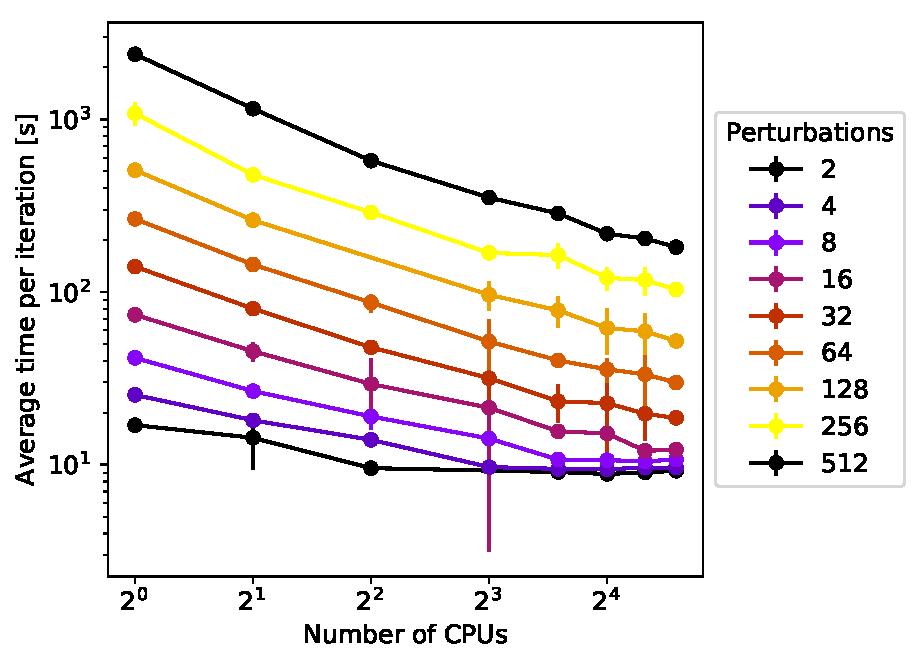
\includegraphics[height=5.7cm]{graphics/E011-sca-analysis/E011-scaling-02.pdf}
        \caption{}
        \label{fig: Theory: E011-scaling-supervised-02}
    \end{subfigure}
    \hfill
    \begin{subfigure}[b]{0.486\textwidth}
        \centering
        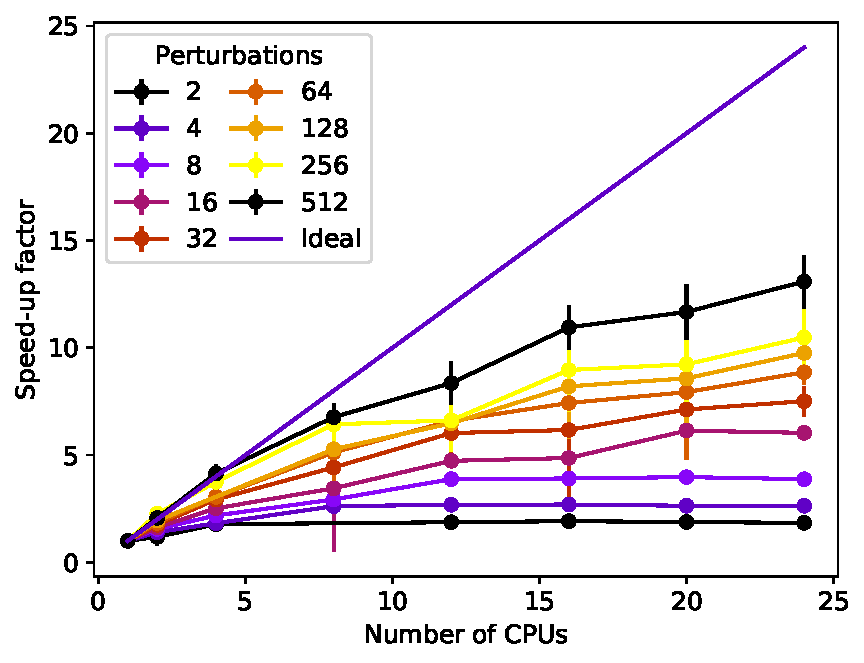
\includegraphics[height=5.7cm]{graphics/E011-sca-analysis/E011-scaling-04.pdf}
        \caption{}
        \label{fig: Theory: E011-scaling-supervised-04}
    \end{subfigure}
    \caption{
        Computational scaling in the reinforcement learning setting for different numbers of \glspl{CPU} and perturbations. Each observation is the average over 100 iterations with associated standard deviation.
        \subref{fig: Theory: E011-scaling-supervised-02} The average time spent per iteration in seconds.
        \subref{fig: Theory: E011-scaling-supervised-04} The observed speedup.
    }
    \label{fig: Theory: E011-scaling-supervised}
\end{figure}

This section presents the results of running the same scaling experiment as before but here on the Atari-2600 game Freeway. The used network is the DQN from \cite{Mnih2015} and preprocessing is as described above. Each episode was limited to 1000 frames (episode horizon) and 100 episodes were simulated for each combination of number of \glspl{CPU} and perturbations. Freeway was chosen since it has a fixed episode duration allowing the use of untrained policies in the experiment. This removes the dependency of the scaling on the quality of the policy.

The results are presented in the same form as for the supervised case in \autoref{fig: Theory: E011-scaling-supervised}. The scaling is somewhat better than for the supervised case and it is achieved for much lower numbers of perturbations as a result of the much more expensive fitness evaluation. For 512 perturbations, increasing the number of \glspl{CPU} from 1 to 4 provides an almost monomial decrease in the time spent per iteration. This is as observed in \cite{Salimans2017} although the computational resources expended for experimentation were much greater than here. Conclusively, reinforcement learning is much more well suited for the \gls{VO} method supervised learning.
%Here, the fitness function evaluation relies on simulation of some often complex environment and the required forward passes of the policy network are inherently sequential.
%!TEX root = ../Thesis.tex


%!TEX root = ../Thesis.tex

\section{Effect of model augmentations and safe mutation}\label{sec: Experimental work: Effects of common model and algorithm augmentations}

\begin{figure}[tbp!]
    \begin{subfigure}[b]{0.49\textwidth}
        \centering
        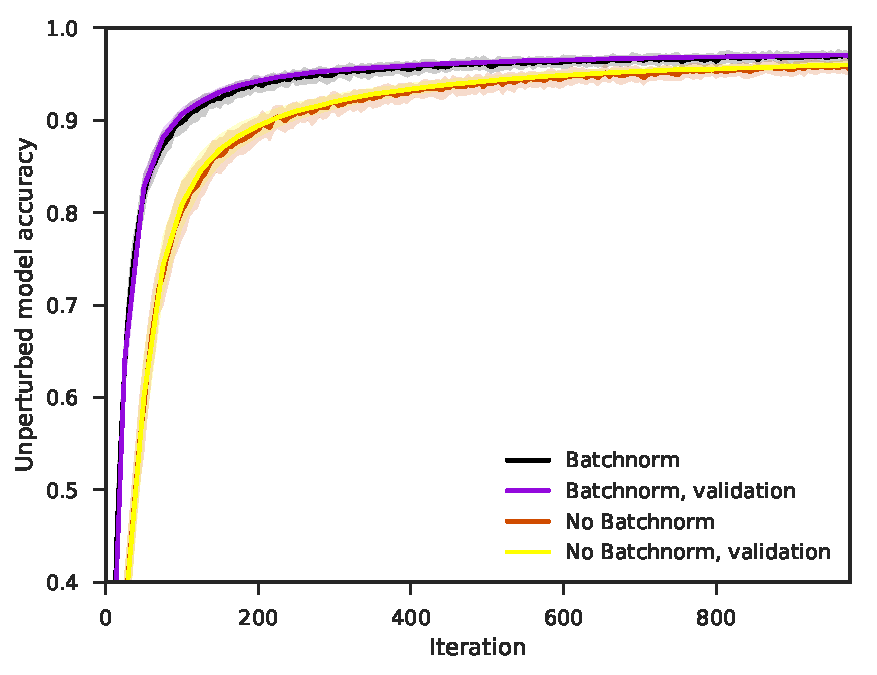
\includegraphics[height=5.8cm]{graphics/E020-bn-analysis/accuracy_unp-all-series-mean-sd.pdf}
        \caption{}
        \label{fig: Theory: E020-bn-analysis/accuracy_unp-all-series-mean-sd}
    \end{subfigure}
    \hfill
    \begin{subfigure}[b]{0.49\textwidth}
        \centering
        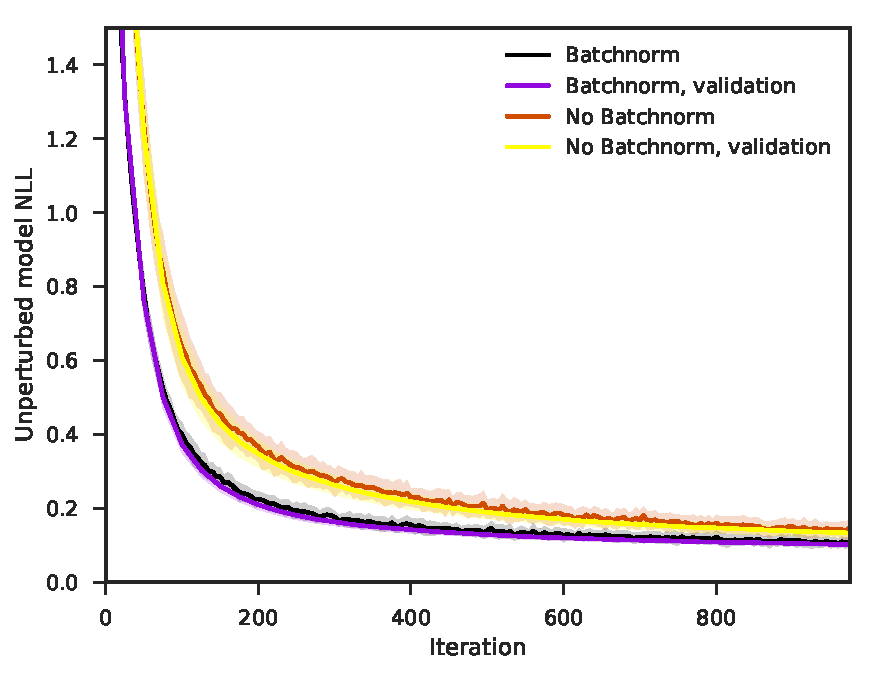
\includegraphics[height=5.8cm]{graphics/E020-bn-analysis/return_unp-all-series-mean-sd.pdf}
        \caption{}
        \label{fig: Theory: E020-bn-analysis/return_unp-all-series-mean-sd}
    \end{subfigure}
    \caption{
        Results of experiments with batch normalization for the unperturbed model.
        \subref{fig: Theory: E020-bn-analysis/accuracy_unp-all-series-mean-sd} Training and validation set classification accuracy.
        \subref{fig: Theory: E020-bn-analysis/return_unp-all-series-mean-sd} Training and validation set \gls{NLL} loss.
        Batch normalization is effective at improving the optimization of the \gls{NN}.
    }
    \label{fig: Theory: E020-bn-analysis}
\end{figure}
This section explores the effects of some common augmentation techniques for \gls{NN} models along with the effects of safe mutation in the \gls{VO} algorithm. The experiments investigate whether the \gls{VO} gradient benefits from the same model improvements as algorithms based on conventional backpropagated gradients do.

The algorithm is isotropic Gaussian \gls{VO} a with fixed variance of $0.05$ similar to \cite{Salimans2017} but uses safe mutation.
%The experiments in this section were performed with the \gls{VO} method listed in \autoref{alg: Canonical variational optimization} using an isotopic Gaussian search distribution but with a fixed $\sigma$ of $0.05$. This algorithm is thus similar to the one used in \cite{Salimans2017} but uses safe mutation.
The experiments were run with 100 perturbations using \gls{SGD} with a momentum of $0.9$ and $L^2$ norm regularization of $0.001$ on all optimized parameters. A learning rate of $0.05$ was used. If nothing else is noted, antithetic sampling and the signed gradient (sum) version of safe mutation were used, batch normalization layers were included in the model and the method of common random numbers was not applied.

The setting is supervised and the data set is \gls{MNIST} for all experiments. The network used is the one for \gls{MNIST} (\autoref{lst: Network models: MNIST with batch normalization}) along with a variant without batch normalization (\autoref{lst: Network models: MNIST without batch normalization}) and a variant without batch normalization and with dropout (\autoref{lst: Network models: MNIST with dropout}).
Each experiment is run for 1000 iterations on mini-batches of 1000 examples for 30 different random seeds. Each experiment shows two plots. The \textbf{(a)} plot shows the classification accuracy for the unperturbed model with each series averaged over the 30 runs at every iteration. The \textbf{(b)} plot shows the \gls{NLL} loss. Both metrics are evaluated on the training set and the test (validation\footnote{The validation set is in fact the remaining part of the data set leaving no data for testing. However, the validation set is not used for fitting any hyperparameters an can as such be regarded a test set as well.}) set during training. The shaded bands indicate one standard deviation among the runs.

Some of these experiments were also run using the Adam optimizer. These plots can be seen in \autoref{app: Effects of common model and algorithm augmentations (Adam optimizer)}. The only difference is the choice of optimizer. The hyperparameter settings for Adam are as recommended in the original paper except for the learning rate which is as for \gls{SGD}. It generally proved to be more difficult to obtain good training characteristics using the Adam optimizer which is hypothesized to be due to the relatively high gradient variance resulting in poor second order moment estimates.


\iffalse
\subsection{Glorot initialization}\label{sec: Experimental work: Glorot initialization}
This section analyzes the results of comparing the default PyTorch initialization scheme with the Glorot initialization scheme \cite{Glorot2010}. \autoref{fig: Theory: E020-init-analysis} shows that initializing the convolutional and linear layers using the Glorot scheme on the \gls{MNIST} network does not yield a signficantly faster learning or better final accuracy compared to the default PyTorch initialization.  In both cases, the learning curves and accuracy curves are almost coincident and within each others standard deviation bands.

That Glorot initialization shows no immediate improvement for the training may here be due to the relatively small network used as well as the simplicity of the problem. Larger networks trained on more challenging data sets may gain more from specialized initialization schemes. Finally, the original paper only applied the scheme to \gls{FNN} without convolutional layers \cite{Glorot2010} which may also influence its effect.

\todo[inline]{WARNING! The default PyTorch initialization is Glorot for linear layers so there really is little difference....}

\begin{figure}[tbp!]
    \begin{subfigure}[b]{0.49\textwidth}
        \centering
        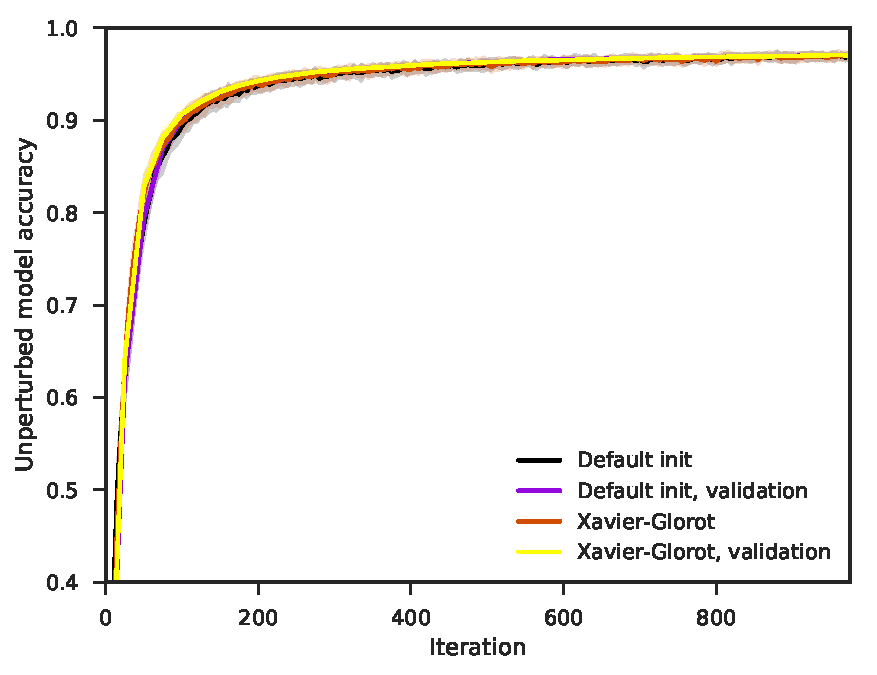
\includegraphics[height=5.8cm]{graphics/E020-init-analysis/accuracy_unp-all-series-mean-sd.pdf}
        \caption{}
        \label{fig: Theory: E020-init-analysis/accuracy_unp-all-series-mean-sd}
    \end{subfigure}
    \hfill
    \begin{subfigure}[b]{0.49\textwidth}
        \centering
        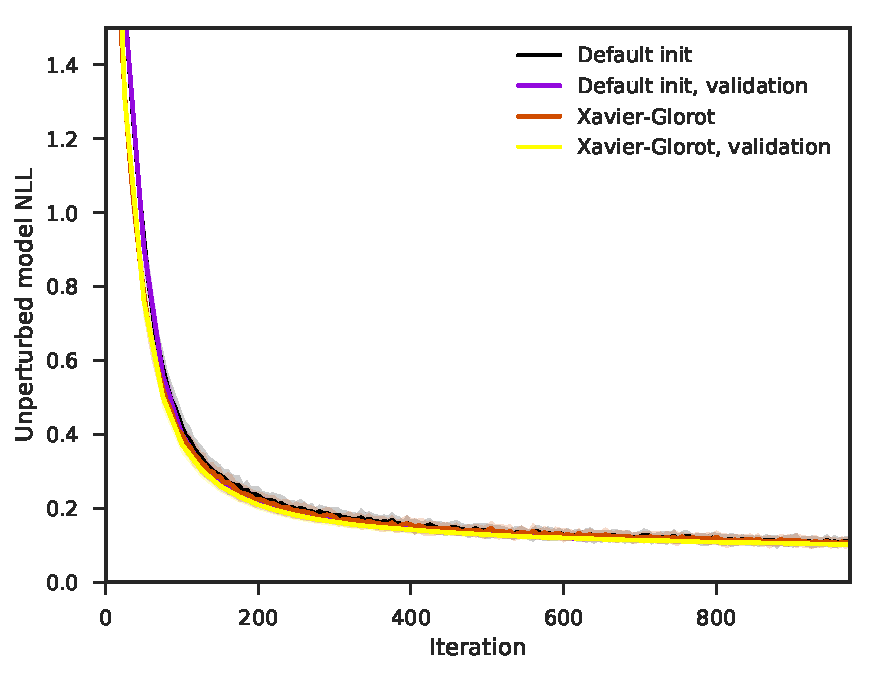
\includegraphics[height=5.8cm]{graphics/E020-init-analysis/return_unp-all-series-mean-sd.pdf}
        \caption{}
        \label{fig: Theory: E020-init-analysis/return_unp-all-series-mean-sd}
    \end{subfigure}
    \caption{
        Results of experiments with initialization scheme for the unperturbed model.
        \subref{fig: Theory: E020-init-analysis/accuracy_unp-all-series-mean-sd} Training and validation set classification accuracy.
        \subref{fig: Theory: E020-init-analysis/return_unp-all-series-mean-sd} Training and validation set \gls{NLL} loss.
    }
    \label{fig: Theory: E020-init-analysis}
\end{figure}
\fi





\subsection{Batch normalization}\label{sec: Experimental work: Batch normalization}
Here, versions of the \gls{MNIST} network with and without batch normalization layers were compared. The positive effect of batch normalization layers between convolution and fully connected layers in the network is evident from \autoref{fig: Theory: E020-bn-analysis}. The network with batch normalization has a significantly steeper loss curve, reaching low losses and high accuracies faster than the network without batch normalization.
It seems the networks asymptote the same final accuracy and loss suggesting that the network without batch normalization is in this case capable of reaching the same level of accuracy as the one with batch normalization, given enough time.
This is in line with the expectated effect of batch normalization as presented in \autoref{chp: Neural networks}. As such, batch normalization can be said to work as expected also with the \gls{VO} gradient which is estimated without the use of backpropagation.



\subsection{Dropout}\label{sec: Experimental work: Dropout}
\begin{figure}[tbp!]
    \begin{subfigure}[b]{0.49\textwidth}
        \centering
        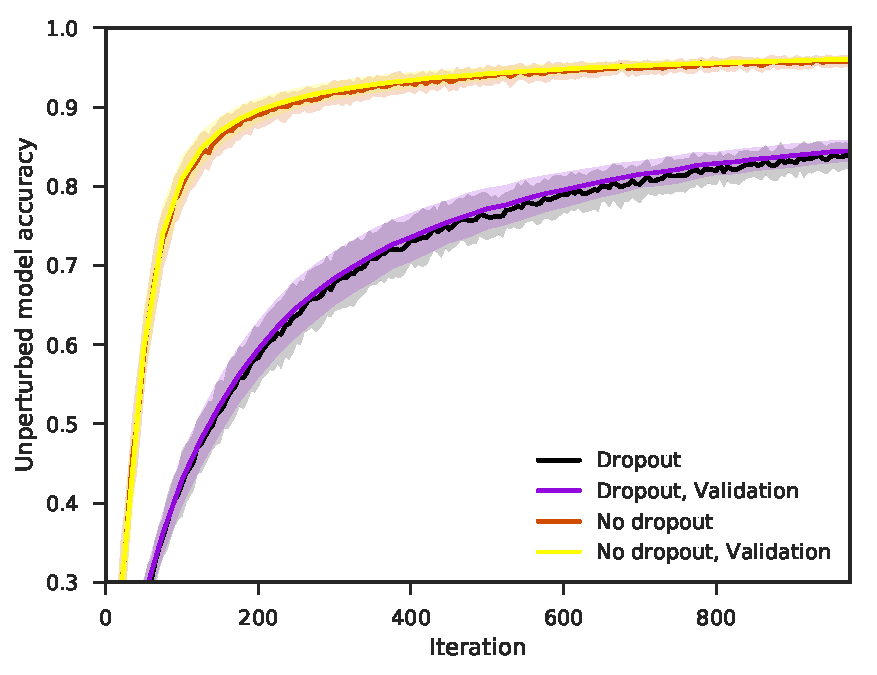
\includegraphics[height=5.8cm]{graphics/E024-DO-SGD-analysis/accuracy_unp-all-series-mean-sd.pdf}
        \caption{}
        \label{fig: Theory: E024-DO-SGD-analysis/accuracy_unp-all-series-mean-sd}
    \end{subfigure}
    \hfill
    \begin{subfigure}[b]{0.49\textwidth}
        \centering
        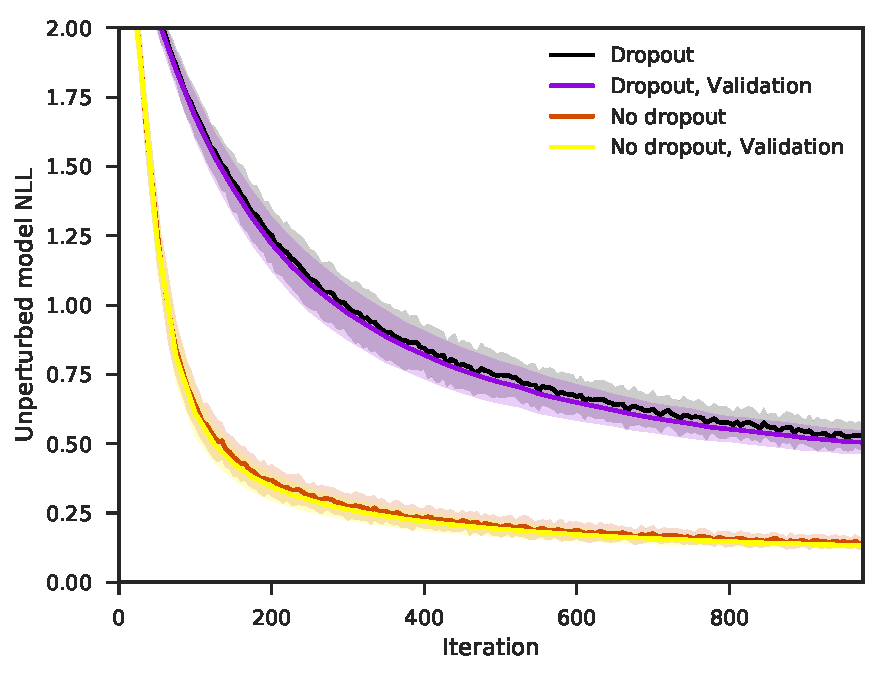
\includegraphics[height=5.8cm]{graphics/E024-DO-SGD-analysis/return_unp-all-series-mean-sd.pdf}
        \caption{}
        \label{fig: Theory: E024-DO-SGD-analysis/return_unp-all-series-mean-sd}
    \end{subfigure}
    \caption{
        Results of experiments with dropout for the unperturbed model.
        \subref{fig: Theory: E024-DO-SGD-analysis/accuracy_unp-all-series-mean-sd} Training and validation set classification accuracy.
        \subref{fig: Theory: E024-DO-SGD-analysis/return_unp-all-series-mean-sd} Training and validation set \gls{NLL} loss. Dropout drastically reduces ease of training probably due to a small network with relatively low capacity and the regularizing effect of optimizing the smoothing \gls{VO} objective.
    }
    \label{fig: Theory: E024-DO-SGD-analysis}
\end{figure}
This section examines the effect of applying dropout to the \gls{MNIST} network. The compared networks are those in \autoref{lst: Network models: MNIST without batch normalization} and \autoref{lst: Network models: MNIST with dropout}, i.e. the network with dropout is compared to a network without dropout. Neither of the networks use batch normalization.

The results of the experiment are shown in \autoref{fig: Theory: E024-DO-SGD-analysis}. The use of dropout results in slower learning and attainment of significantly inferior loss and classification accuracy withing the 1000 iterations. This effect of using dropout is expected to some degree since for the relatively small network used, randomly zeroing weights can drastically reduce model capacity.
Additionally, the \gls{MNIST} network without dropout showed no signs of overfitting in other experiments using the stochastic gradient estimate. As such, dropout was not expected to be able to radically improve performance. 

The fact that no overfitting occurs for this model may be linked to the smoothing of the objective function imposed by using the variational objective. This is most likely a different perspective on the fact that \gls{VO} with a fixed variance optimizes for the average loss of the entire population of perturbations \cite{Lehman2017}. It seems probable that this assists in avoiding overfitting. This observation is also in line with the examples of \autoref{fig: Theory: var-opt-conv-ES-himmelblau}, \ref{fig: Theory: var-opt-conv-VO-R-himmelblau} and \ref{fig: Theory: var-opt-conv-VO-N-himmelblau} where the algorithm with fixed $\sigma$ cannot fully converge on the minimum, and in some sense, thus cannot not overfit it.

\subsection{Safe mutation}
\begin{figure}[tbp!]
    \begin{subfigure}[b]{0.49\textwidth}
        \centering
        \includegraphics[height=5.8cm]{graphics/E021-SM-analysis/accuracy_unp-all-series-mean-sd.pdf}
        \caption{}
        \label{fig: Theory: E021-SM-analysis/accuracy_unp-all-series-mean-sd}
    \end{subfigure}
    \hfill
    \begin{subfigure}[b]{0.49\textwidth}
        \centering
        \includegraphics[height=5.8cm]{graphics/E021-SM-analysis/return_unp-all-series-mean-sd.pdf}
        \caption{}
        \label{fig: Theory: E021-SM-analysis/return_unp-all-series-mean-sd}
    \end{subfigure}
    \caption{
        Results of experiments with safe mutation (SM-G-SUM) for the unperturbed model.
        \subref{fig: Theory: E021-SM-analysis/accuracy_unp-all-series-mean-sd} Training and validation set classification accuracy.
        \subref{fig: Theory: E021-SM-analysis/return_unp-all-series-mean-sd} Training and validation set \gls{NLL} loss.
        Scaling perturbations according to network parameter sensitivities results in more stable training.
    }
    \label{fig: Theory: E021-SM-analysis}
\end{figure}
This section compares runs with and without the signed gradient (sum) version of safe mutation \cite{Lehman2017a}.

The results are shown in \autoref{fig: Theory: E021-SM-analysis}. Considering the loss curves, not using safe mutation results in much higher variance among runs with different seeds and yields an over run average loss that is much higher compared to runs using safe mutation. Considering the classification accuracies, the difference between runs with and without safe mutation is smaller although the same trends are observed: Over run variance is higher without safe mutation than it is with and runs without safe mutation reach lower classification accuracies on average. This, along with the high loss, indicates that the variants without safe mutation end up in relatively poor areas of the loss surfaces.

It should be noted that it cannot be ruled out that a lower learning rate exists that allows better performance without safe mutation than what is observed here. For instance, the results presented in \cite{Salimans2017} did not use safe mutation. In this case, the use of safe mutation effectively allows using a higher learning rate which must be expected to result in faster convergence.

\newpage
%!TEX root = ../Thesis.tex

\section{Methods for variance reduction}
This section explores the effects of different variance reduction methods. If nothing else is noted, the training details are as described in \autoref{sec: Experimental work: Effects of common model and algorithm augmentations}.

\subsection{Gradient momentum}\label{sec: Experimental work: Effect of momentum}
Due to the potentially high variance of the \gls{VO} gradient, the use of momentum (see \autoref{sec: Neural networks training: Optimization: SGD with momentum}) can have a positive effect on the convergence speed and training time of \gls{VO}. Three levels of momentum were run for thirty random seeds each. The momentums were $0$, $0.1$ and $0.9$. The results can be seen in \autoref{fig: Theory: E030-MOM-S-analysis}. 
A small benefit can be noted from using a momentum of $0.1$ while using $0.9$ has a large impact on the convergence speed.
It is evident that the \gls{VO} gradient benefits from including momentum.

A momentum of $0.99$ was also included in this experiment but resulted in the algorithm not converging. Instead, the training achieved losses of about $0.6$, oscillating up and down presumably due to the gradient being too dependent on past values to adequately adapt to the loss surface. It is plausible that an optimal value of the momentum for this problem resides somewhere between $0.99$ and $0.1$ but no attempt will be made at finding this value.

When adapting the variance, the effect of momentum on the variance was also examined and found to occasionally be detrimental, especially in the \gls{RL} setting. At times, the gradient associated with the variance would spike at a single iteration, preceded and followed by much smaller gradients. Momentum would then continue to increase the variance for many iterations following the spike resulting in a large variance giving detrimentally large perturbations. Lowering the variance learning rate results in the variance practically not adapting during training. Using dampened momentum aids in suppressing these spikes and is discussed further in \autoref{sec: Experimental work: Effect of adapting the variance}. Alternatively, not using momentum on the variance gradient gives little weight to these spikes and the trend of decreasing variance persists through training as wanted.

\begin{figure}[tbp!]
    \begin{subfigure}[b]{0.49\textwidth}
        \centering
        \includegraphics[height=5.8cm]{graphics/E030-MOM-S-analysis/accuracy_unp-all-series-mean-sd.pdf}
        \caption{}
        \label{fig: Theory: E030-MOM-S-analysis/accuracy_unp-all-series-mean-sd}
    \end{subfigure}
    \hfill
    \begin{subfigure}[b]{0.49\textwidth}
        \centering
        \includegraphics[height=5.8cm]{graphics/E030-MOM-S-analysis/return_unp-all-series-mean-sd.pdf}
        \caption{}
        \label{fig: Theory: E030-MOM-S-analysis/return_unp-all-series-mean-sd}
    \end{subfigure}
    \caption{
        Results of experiments using \gls{SGD} with momentum on the \gls{VO} gradient for the unperturbed model run on \gls{MNIST}.
        \subref{fig: Theory: E030-MOM-S-analysis/accuracy_unp-all-series-mean-sd} Training and validation set classification accuracy.
        \subref{fig: Theory: E030-MOM-S-analysis/return_unp-all-series-mean-sd} Training and validation set \gls{NLL} loss.
        Gradient momentum is effective at reducing the gradient variance and results in faster convergence.
    }
    \label{fig: Theory: E030-MOM-S-analysis}
\end{figure}


\subsection{Antithetic sampling}\label{sec: Experimental work: Antithetic sampling}
In this section, the improvement by using antithetic sampling is experimentally validated. The \gls{MNIST} network was trained using 100 perturbations with antithetic sampling (50 unique, 50 mirrored), 100 perturbations without antithetic sampling and 50 perturbations without antithetic sampling. 

The runs using 100 perturbations with antithetic sampling compares to the runs using 100 perturbations without antithetic sampling in the way that both estimate the gradient from 100 perturbations. From this comparison it can be assessed whether the antithetic samples carry more information than the regular uninformed samples.

The grounds for comparison of runs using 50 perturbations without and 100 perturbations with antithetic sampling is that both of these versions perturb an 50-dimensional subspace of the network parameter space at every iteration of \glsfirst{VO}.
Additionally, the computational complexity of sampling is half as high when using antithetic sampling.
Obviously, the time complexity of the sampling operation is negligible compared to the fitness evaluation so comparison in this basis is not entirely fair.

The results are shown in \autoref{fig: Theory: E022-AS-analysis}. It is evident that using antithetic sampling results in a significant improvement when comparing to both runs with 50 and 100 perturbations. As opposed to the effect seen when including batch normalization, the loss curves initially rise with approximately the same slope but do not asymptote the same value. Thus, the benefit from using antithetic sampling is not faster training but rather the location of a better local minimum and thus better final performance. This is almost certainly due to a reduction in the gradient estimate variance. 

\begin{figure}[tbp!]
    \begin{subfigure}[b]{0.49\textwidth}
        \centering
        \includegraphics[height=5.8cm]{graphics/E022-AS-analysis/accuracy_unp-all-series-mean-sd.pdf}
        \caption{}
        \label{fig: Theory: E022-AS-analysis/accuracy_unp-all-series-mean-sd}
    \end{subfigure}
    \hfill
    \begin{subfigure}[b]{0.49\textwidth}
        \centering
        \includegraphics[height=5.8cm]{graphics/E022-AS-analysis/return_unp-all-series-mean-sd.pdf}
        \caption{}
        \label{fig: Theory: E022-AS-analysis/return_unp-all-series-mean-sd}
    \end{subfigure}
    \caption{
        Results of experiments with antithetic sampling for the unperturbed model.
        \subref{fig: Theory: E022-AS-analysis/accuracy_unp-all-series-mean-sd} Training and validation set classification accuracy.
        \subref{fig: Theory: E022-AS-analysis/return_unp-all-series-mean-sd} Training and validation set \gls{NLL} loss.
    }
    \label{fig: Theory: E022-AS-analysis}
\end{figure}

\subsection{Importance mixing}
This section presents results of using importance mixing. This comparison is made in spite of the importance weight collapse and the numerical problems associated with it. In practice some weights become infinite which leads to some reuse of some perturbations. 

\autoref{fig: Theory: E025-IS-analysis} compares a run with importance mixing $(\alpha=0.01)$ and a run without $(\alpha=1.0)$. The \gls{NLL} when using importance mixing is slightly higher than when not. This observation is present in the resulting classification accuracy as well. This detrimental effect must be concluded to stem from the collapse of the importance weights as previously discussed.

\begin{figure}[tbp!]
    \begin{subfigure}[b]{0.49\textwidth}
        \centering
        \includegraphics[height=5.8cm]{graphics/E025-IS-analysis/accuracy_unp-all-series-mean-sd.pdf}
        \caption{}
        \label{fig: Theory: E025-IS-analysis/accuracy_unp-all-series-mean-sd}
    \end{subfigure}
    \hfill
    \begin{subfigure}[b]{0.49\textwidth}
        \centering
        \includegraphics[height=5.8cm]{graphics/E025-IS-analysis/return_unp-all-series-mean-sd.pdf}
        \caption{}
        \label{fig: Theory: E025-IS-analysis/return_unp-all-series-mean-sd}
    \end{subfigure}
    \caption{
        Results of experiments with importance mixing for the unperturbed model.
        \subref{fig: Theory: E025-IS-analysis/accuracy_unp-all-series-mean-sd} Training and validation set classification accuracy.
        \subref{fig: Theory: E025-IS-analysis/return_unp-all-series-mean-sd} Training and validation set \gls{NLL} loss.
    }
    \label{fig: Theory: E025-IS-analysis}
\end{figure}

For comparison, \autoref{fig: Theory: E026-IS-analysis} presents results runs where importance mixing has been replaced by random reuse of perturbations. In the runs with importance mixing, about 10 of the 100 perturbations where effectively reused at each iteration. Therefore, the experiment with random reuse reused 10 perturbations randomly at each iteration. It can be observed that the effect of randomly reusing perturbations is smaller than that of importance mixing, although it remains detrimental compared to reusing no perturbations.

\begin{figure}[tbp!]
    \begin{subfigure}[b]{0.49\textwidth}
        \centering
        \includegraphics[height=5.8cm]{graphics/E026-IS-analysis/accuracy_unp-all-series-mean-sd.pdf}
        \caption{}
        \label{fig: Theory: E026-IS-analysis/accuracy_unp-all-series-mean-sd}
    \end{subfigure}
    \hfill
    \begin{subfigure}[b]{0.49\textwidth}
        \centering
        \includegraphics[height=5.8cm]{graphics/E026-IS-analysis/return_unp-all-series-mean-sd.pdf}
        \caption{}
        \label{fig: Theory: E026-IS-analysis/return_unp-all-series-mean-sd}
    \end{subfigure}
    \caption{
        Results of experiments with random resampling for the unperturbed model.
        \subref{fig: Theory: E026-IS-analysis/accuracy_unp-all-series-mean-sd} Training and validation set classification accuracy.
        \subref{fig: Theory: E026-IS-analysis/return_unp-all-series-mean-sd} Training and validation set \gls{NLL} loss.
    }
    \label{fig: Theory: E026-IS-analysis}
\end{figure}

One can note that randomly reusing perturbations is likely to break to assumption that the set of perturbations follows the search distribution, i.e. the Gaussian in this case. Since the gradient estimators rely on this assumption, the detrimental effect of random reuse of perturbations is expected. Importance mixing is designed to maintain the distribution of the perturbations but due to the collapse of the importance weights this is not the case in practice.






% \subsection{Adaptation sampling}
% \todo[inline]{Run the experiment on using adaptation sampling on \gls{MNIST} model}
% \todo[inline]{Discuss experimental results of adaptation sampling}





\subsection{Common random numbers}
This section presents results using the method of \gls{CRN}. The \gls{MNIST} network was trained using 100 perturbations with and without \gls{CRN} resulting in the training curves illustrated in \autoref{fig: Theory: E027-CRN-S-analysis}. \gls{CRN} was also tested in the \gls{RL} setting with resulting learning curves seen in \autoref{fig: Theory: E028-CRN-R-analysis}. The \gls{RL} runs were made using 40 perturbations for computational feasibility.

There is a small and almost insignificant benefit to using \gls{CRN} in the case of supervised learning on \gls{MNIST}. It can be seen that using \gls{CRN}, the training and validation accuracy and loss slightly outperform those of runs that did not use \gls{CRN} on average but within one standard deviation.

The method was also tested in the \gls{RL} setting with $45$ episodes simulated for each of the shared and random seeds versions.
The results are seen for Freeway in \autoref{fig: Theory: E028-CRN-R1-analysis/return_unp-all-series-mean-sd} and  Seaquest in \autoref{fig: Theory: E028-CRN-R2-analysis/return_unp-all-series-mean-sd}. The average population reward is plotted versus iteration number. 
The picture is similar to that of supervised learning with no significant improvement to be seen by using shared seeds for the simulations. 
As such, the method of \gls{CRN} cannot be concluded to improve on the \gls{VO} gradient estimate.

\begin{figure}[tbp!]
    \begin{subfigure}[b]{0.49\textwidth}
        \centering
        \includegraphics[height=5.7cm]{graphics/E027-CRN-S-analysis/accuracy_unp-all-series-mean-sd.pdf}
        \caption{}
        \label{fig: Theory: E027-CRN-S-analysis/accuracy_unp-all-series-mean-sd}
    \end{subfigure}
    \hfill
    \begin{subfigure}[b]{0.49\textwidth}
        \centering
        \includegraphics[height=5.7cm]{graphics/E027-CRN-S-analysis/return_unp-all-series-mean-sd.pdf}
        \caption{}
        \label{fig: Theory: E027-CRN-S-analysis/return_unp-all-series-mean-sd}
    \end{subfigure}
    \caption{
        Results of experiments with \glsfirst{CRN} for the unperturbed model run on \gls{MNIST}.
        \subref{fig: Theory: E027-CRN-S-analysis/accuracy_unp-all-series-mean-sd} Training and validation set classification accuracy.
        \subref{fig: Theory: E027-CRN-S-analysis/return_unp-all-series-mean-sd} Training and validation set \gls{NLL} loss.
    }
    \label{fig: Theory: E027-CRN-S-analysis}
\end{figure}
\begin{figure}[tbp!]
    \begin{subfigure}[b]{0.49\textwidth}
        \centering
        \includegraphics[height=5.8cm]{graphics/E028-CRN-R1-analysis/return_avg-all-series-mean-sd.pdf}
        \caption{}
        \label{fig: Theory: E028-CRN-R1-analysis/return_unp-all-series-mean-sd}
    \end{subfigure}
    \hfill
    \begin{subfigure}[b]{0.49\textwidth}
        \centering
        \includegraphics[height=5.8cm]{graphics/E028-CRN-R2-analysis/return_avg-all-series-mean-sd.pdf}
        \caption{}
        \label{fig: Theory: E028-CRN-R2-analysis/return_unp-all-series-mean-sd}
    \end{subfigure}
    \caption{
        Results of experiments with \glsfirst{CRN} for the population average on \subref{fig: Theory: E028-CRN-R1-analysis/return_unp-all-series-mean-sd} Freeway and \subref{fig: Theory: E028-CRN-R2-analysis/return_unp-all-series-mean-sd} Seaquest. The average reward of the population is plotted as a function of \gls{VO} iterations.
    }
    \label{fig: Theory: E028-CRN-R-analysis}
\end{figure}



%!TEX root = ../Thesis.tex

\section{Effect of adapting the variance}\label{sec: Experimental work: Effect of adapting the variance}
Until now, all experiments have been run with an isotropic Gaussian with fixed variance similarly to \cite{Salimans2017}. Here, different variants of the Gaussian search distribution with adaptive variance will be examined.
The examined variants are the isotropic Gaussian, the layer-wise separable Gaussian and the parameter-wise separable Gaussian. For the layer-wise separable Gaussian, a single variance parameter is used for each weight/kernel matrix and bias vector in the model.
Hyperparameters are otherwise as in \autoref{sec: Experimental work: Effects of common model and algorithm augmentations}.

For these experiments, a momentum of $0.9$ has been used on the parameter gradient as well as the adapted variance gradient while the variance gradient is also dampened by $0.9$. Dampening the variance gradient makes sure it does not spike as discussed in \autoref{sec: Experimental work: Effect of momentum}. Dampened momentum on the variance gradient results in much smoother updates to the variance than applying no momentum or non-dampened momentum. Learning rates of $2$ and $4$ have been used for the isotropic and separable Gaussian variances, respectively.


\subsection{Adapting the variance}
\autoref{fig: Theory: E029-VO-S5-MD-analysis} shows the results of running the \gls{VO} algorithm on the MNIST network with the different search distributions. 
\autoref{fig: Theory: E029-VO-S5-MD-analysis/accuracy_val-all-series-mean-sd} and \ref{fig: Theory: E029-VO-S5-MD-analysis/return_val-all-series-mean-sd} respectively show the validation set accuracy and \gls{NLL} loss for the different search distributions.
The most notable difference between the variations is that when the variance is adapted, the isotropic Gaussian gives somewhat unstable learning, in that it gives quite different results solely dependent on random seed.
This can be seen not to be the case when adapting a layer- or parameter-wise separable Gaussians. 

Despite this, the convergence rate and the median final \gls{NLL} loss and accuracy are not improved when using these adaptive search distributions compared to using the fixed isotropic Gaussian. 
Considering the single best and worst performing models on the validation set, it can be noted that these are all obtained by the separable versions. As such, adapting the variance seems to encourage more extensive exploration of the loss landscape but with risk of landing in both a slightly better and slightly worse minimum than would have been reached with a fixed variance.

It should be noted that these observations hold for many different learning rates for the variance parameter(s).

\begin{figure}[tbp!]
    \begin{subfigure}[b]{0.49\textwidth}
        \centering
        \includegraphics[height=5.8cm]{graphics/E029-VO-S5-MD-analysis/accuracy_val-all-series-mean-sd.pdf}
        \caption{}
        \label{fig: Theory: E029-VO-S5-MD-analysis/accuracy_val-all-series-mean-sd}
    \end{subfigure}
    \hfill
    \begin{subfigure}[b]{0.49\textwidth}
        \centering
        \includegraphics[height=5.8cm]{graphics/E029-VO-S5-MD-analysis/return_val-all-series-mean-sd.pdf}
        \caption{}
        \label{fig: Theory: E029-VO-S5-MD-analysis/return_val-all-series-mean-sd}
    \end{subfigure}
    \begin{subfigure}[b]{0.49\textwidth}
        \centering
        \includegraphics[height=5.3cm]{graphics/E029-VO-S5-MD-analysis/accuracy-final-distribution-boxplot-grouped.pdf}
        \caption{}
        \label{fig: Theory: E029-VO-S5-MD-analysis/accuracy-final-distribution-boxplot-grouped}
    \end{subfigure}
    \hfill
    \begin{subfigure}[b]{0.49\textwidth}
        \centering
        \includegraphics[height=5.3cm]{graphics/E029-VO-S5-MD-analysis/return-final-distribution-boxplot-grouped.pdf}
        \caption{}
        \label{fig: Theory: E029-VO-S5-MD-analysis/return-final-distribution-boxplot-grouped}
    \end{subfigure}
    \caption{
        Results of experiments with different \gls{VO} algorithms. The model variations are the fixed variance strategy of \cite{Salimans2017} and \gls{VO} with adjusted variance using an isotropic Gaussian and respectively a layer-wise and per-weight separable Gaussian. Contrary to \cite{Salimans2017}, safe mutation is applied.
        Plotted versus the iteration number, \subref{fig: Theory: E029-VO-S5-MD-analysis/accuracy_val-all-series-mean-sd} shows the validation set classification accuracy and \subref{fig: Theory: E029-VO-S5-MD-analysis/return_val-all-series-mean-sd} the validation set \gls{NLL} loss. 
        Difference in performance between the algorithms is very small and within one standard deviation with the adapted isotropic having high between-run variance.
        In \subref{fig: Theory: E029-VO-S5-MD-analysis/accuracy-final-distribution-boxplot-grouped} and \subref{fig: Theory: E029-VO-S5-MD-analysis/return-final-distribution-boxplot-grouped} the final distribution of the classification accuracy and \gls{NLL} loss from \subref{fig: Theory: E029-VO-S5-MD-analysis/accuracy_val-all-series-mean-sd} and \subref{fig: Theory: E029-VO-S5-MD-analysis/return_val-all-series-mean-sd} are shown. It can be noted that adapting the variance in the isotropic Gaussian search distribution results a much wider span of the final \gls{NLL} loss. Additionally, a small group of runs has an even higher final \gls{NLL} loss than the main body of runs. This is not observed for the other versions.
        %These seem to hint at a potential better final performance by adapting the variance of a layer-wise separable Gaussian search distribution.
        %which is more flexible than an isotropic Gaussian but has fewer parameters and is easier to estimate than a separable Gaussian with per-weight variances.
    }
    \label{fig: Theory: E029-VO-S5-MD-analysis}
\end{figure}


% \begin{figure}[tbp!]
%     \begin{subfigure}[b]{0.49\textwidth}
%         \centering
%         \includegraphics[height=5.8cm]{graphics/E029-VO-S3-analysis-1500/accuracy_val-all-series-mean-sd.pdf}
%         \caption{}
%         \label{fig: Theory: E029-VO-S3-analysis-1500/accuracy_val-all-series-mean-sd}
%     \end{subfigure}
%     \hfill
%     \begin{subfigure}[b]{0.49\textwidth}
%         \centering
%         \includegraphics[height=5.8cm]{graphics/E029-VO-S3-analysis-1500/return_val-all-series-mean-sd.pdf}
%         \caption{}
%         \label{fig: Theory: E029-VO-S3-analysis-1500/return_val-all-series-mean-sd}
%     \end{subfigure}
%     \begin{subfigure}[b]{0.49\textwidth}
%         \centering
%         \includegraphics[height=5.3cm]{graphics/E029-VO-S3-analysis-1500/accuracy-final-distribution-boxplot-grouped.pdf}
%         \caption{}
%         \label{fig: Theory: E029-VO-S3-analysis-1500/accuracy-final-distribution-boxplot-grouped}
%     \end{subfigure}
%     \hfill
%     \begin{subfigure}[b]{0.49\textwidth}
%         \centering
%         \includegraphics[height=5.3cm]{graphics/E029-VO-S3-analysis-1500/return-final-distribution-boxplot-grouped.pdf}
%         \caption{}
%         \label{fig: Theory: E029-VO-S3-analysis-1500/return-final-distribution-boxplot-grouped}
%     \end{subfigure}
%     \caption{
%         Results of experiments with different \gls{VO} algorithms. The model variations are the fixed variance strategy of \cite{Salimans2017} and \gls{VO} with adjusted variance using an isotropic Gaussian and respectively a layer-wise and per-weight separable Gaussian. Contrary to \cite{Salimans2017}, safe mutation is applied.
%         Plotted versus the iteration number \subref{fig: Theory: E029-VO-S3-analysis-1500/accuracy_val-all-series-mean-sd} shows the validation set classification accuracy and \subref{fig: Theory: E029-VO-S3-analysis-1500/return_val-all-series-mean-sd} the validation set \gls{NLL} loss. 
%         Difference in performance between the algorithms is very small and certainly insignificant.
%         In \subref{fig: Theory: E029-VO-S3-analysis-1500/accuracy-final-distribution-boxplot-grouped} and \subref{fig: Theory: E029-VO-S3-analysis-1500/return-final-distribution-boxplot-grouped} the final distribution of the classification accuracy and \gls{NLL} loss from \subref{fig: Theory: E029-VO-S3-analysis-1500/accuracy_val-all-series-mean-sd} and \subref{fig: Theory: E029-VO-S3-analysis-1500/return_val-all-series-mean-sd} are shown.
%         %These seem to hint at a potential better final performance by adapting the variance of a layer-wise separable Gaussian search distribution.
%         %which is more flexible than an isotropic Gaussian but has fewer parameters and is easier to estimate than a separable Gaussian with per-weight variances.
%     }
%     \label{fig: Theory: E029-VO-S3-analysis-1500}
% \end{figure}


% \begin{figure}[tbp!]
%     \begin{subfigure}[b]{0.49\textwidth}
%         \centering
%         \includegraphics[height=5.8cm]{graphics/E029-VO-S2-analysis/accuracy_val-all-series-mean-sd.pdf}
%         \caption{}
%         \label{fig: Theory: E029-VO-S2-analysis/accuracy_val-all-series-mean-sd}
%     \end{subfigure}
%     \hfill
%     \begin{subfigure}[b]{0.49\textwidth}
%         \centering
%         \includegraphics[height=5.8cm]{graphics/E029-VO-S2-analysis/return_val-all-series-mean-sd.pdf}
%         \caption{}
%         \label{fig: Theory: E029-VO-S2-analysis/return_val-all-series-mean-sd}
%     \end{subfigure}
%     \begin{subfigure}[b]{0.49\textwidth}
%         \centering
%         \includegraphics[height=5.2cm]{graphics/E029-VO-S2-analysis/accuracy_val-final-distribution-boxplot.pdf}
%         \caption{}
%         \label{fig: Theory: E029-VO-S2-analysis/accuracy_val-final-distribution-boxplot}
%     \end{subfigure}
%     \hfill
%     \begin{subfigure}[b]{0.49\textwidth}
%         \centering
%         \includegraphics[height=5.2cm]{graphics/E029-VO-S2-analysis/return_val-final-distribution-boxplot.pdf}
%         \caption{}
%         \label{fig: Theory: E029-VO-S2-analysis/return_val-final-distribution-boxplot}
%     \end{subfigure}
%     \caption{
%         Results of experiments with different \gls{VO} algorithms. The plots all show the validation \gls{NLL} or the validation classification accuracy of the unperturbed model. The model variations are the fixed variance strategy of \cite{Salimans2017} and \gls{VO} with adjusted variance using an isotropic Gaussian and respectively a layer-wise and per-weight separable Gaussian.
%         Plotted versus the iteration number \subref{fig: Theory: E029-VO-S2-analysis/accuracy_val-all-series-mean-sd} shows the validation set classification accuracy and \subref{fig: Theory: E029-VO-S2-analysis/return_val-all-series-mean-sd} the validation set \gls{NLL} loss. Difference in performance between the algorithms is very small and certainly insignificant.
%         In \subref{fig: Theory: E029-VO-S2-analysis/accuracy_val-final-distribution-boxplot} and \subref{fig: Theory: E029-VO-S2-analysis/return_val-final-distribution-boxplot} the final distribution of the classification accuracy and \gls{NLL} loss from \subref{fig: Theory: E029-VO-S2-analysis/accuracy_val-all-series-mean-sd} and \subref{fig: Theory: E029-VO-S2-analysis/return_val-all-series-mean-sd} are shown. These seem to hint at a potential better final performance by adapting the variance of a layer-wise separable Gaussian search distribution.
%         %which is more flexible than an isotropic Gaussian but has fewer parameters and is easier to estimate than a separable Gaussian with per-weight variances.
%     }
%     \label{fig: Theory: E029-VO-S2-analysis}
% \end{figure}







\subsection{The gradient norm}
This section examines the interaction between adapting the variance and the norm of the \gls{VO} gradient and the parameter vector in order to shed more light on the effect of adapting the variance. It does so based on single runs of the training, but it should be noted that the observations hold generally for additional runs with different random seeds.

Consider the gradient and parameter norms when using an isotropic Gaussian search distribution. 
As can be seen from the derived \gls{VO} gradient estimators in \eqref{eq: Theory: Variational optimization multivariate isotropic gaussian gradient estimators}, the gradient is scaled by the variance.
In case the variance is fixed, this is obviously a constant scaling factor.
However, when adapting the variance, this effectively scales the term computed by the sum differently at each iteration. It is evident that the variance then has a direct adaptive effect on the gradient norm and thus affects the iteration step size. The effect that the variance has through multiplication on the perturbation and indirectly through the value of the objective function is harder to determine. Since the perturbations are from a standard Gaussian, multiplying them by $\sigma$ does not change their expectation. Additionally, it is theoretically possible for the objective function to both increase and decrease in value for any size of the perturbation. However, very large perturbations must be expected to result in catastrophic forgetting in the perturbed networks as any learned filters etc. are washed out with noise.

\begin{figure}[tbp!]
    \begin{subfigure}[b]{0.49\textwidth}
        \centering
        \includegraphics[height=5.5cm]{graphics/E031-NORM-analysis/isotropic-fixed-1-param-and-grad-and-variance-norm.pdf}
        \caption{}
        \label{fig: Theory: E031-NORM-analysis/isotropic-fixed-1-param-and-grad-and-variance-norm}
    \end{subfigure}
    \hfill
    \begin{subfigure}[b]{0.49\textwidth}
        \centering
        \includegraphics[height=5.5cm]{graphics/E031-NORM-analysis/isotropic-adapted-1-param-and-grad-and-variance-norm.pdf}
        \caption{}
        \label{fig: Theory: E031-NORM-analysis/isotropic-adapted-1-param-and-grad-and-variance-norm}
    \end{subfigure}
    \caption{
        2-norms of the \gls{NN} parameter vector and \gls{VO} gradient for an isotropic Gaussian search distribution with the variance overlayed (multiplied by 100 for scale). In \subref{fig: Theory: E031-NORM-analysis/isotropic-fixed-1-param-and-grad-and-variance-norm} and \subref{fig: Theory: E031-NORM-analysis/isotropic-adapted-1-param-and-grad-and-variance-norm}, the fixed and adapted variance versions are shown, respectively. A centered $50$ sample moving average is computed for the gradient. It is clear that adapting the variance directly and significantly influences the norm of the gradient and in turn also the norm of the parameter vector.
    }
    \label{fig: Theory: E031-NORM-analysis-isotropic}
\end{figure}
The gradient and parameter norms for fixed and adapted variance isotropic Gaussians are plotted in \autoref{fig: Theory: E031-NORM-analysis-isotropic} for a single run of the \gls{MNIST} network (\autoref{lst: Network models: MNIST with batch normalization}). The variance is overlaid in the plots as well. 
A fixed variance (\ref{fig: Theory: E031-NORM-analysis/isotropic-fixed-1-param-and-grad-and-variance-norm}) results in a gradient that rapidly reaches a constant level. The parameter norm increases fairly steadily as a result, but seems to plateau when a minimum is found\footnote{The learning curves are similar to the ones in \autoref{fig: Theory: E029-VO-S5-MD-analysis}}. Interestingly enough, the gradient does not go to zero as the minimum is reached but remains relatively high. This is in-line with the rarity of local minima and the prevalence of saddle points as previously mentioned.
It should be noted that the small amount of $L^2$ regularization adds to decrease the parameter norm. By adapting the variance (\ref{fig: Theory: E031-NORM-analysis/isotropic-adapted-1-param-and-grad-and-variance-norm}), the gradient is also adapted: As the variance decreases so does the gradient norm and in turn the parameter norm as well. The effect of the variance on the gradient norm is similar to that of adaptively decreasing the learning rate during training in the way that increasingly smaller steps are taken as training progresses. By inspecting the results presented in \autoref{fig: Theory: E029-VO-S5-MD-analysis}, it was found that the small poorly performing group of runs that used the adapted isotropic Gaussian had a variance that generally increased rather than decreased throughout training. This then directly resulted in larger gradients and in turn divergence.

\begin{figure}[tbp!]
    \begin{subfigure}[b]{0.49\textwidth}
        \centering
        \includegraphics[height=5.6cm]{graphics/E031-NORM-analysis/separable-layer-5-param-and-grad-norm.pdf}
        \caption{}
        \label{fig: Theory: E031-NORM-analysis/separable-layer-5-param-and-grad-norm}
    \end{subfigure}
    \hfill
    \begin{subfigure}[b]{0.49\textwidth}
        \centering
        \includegraphics[height=5.6cm]{graphics/E031-NORM-analysis/separable-layer-5-variance.pdf}
        \caption{}
        \label{fig: Theory: E031-NORM-analysis/separable-layer-5-variance}
    \end{subfigure}
    \caption{
        \subref{fig: Theory: E031-NORM-analysis/separable-layer-5-param-and-grad-norm} 2-norms of the \gls{NN} parameter vector and \gls{VO} gradient for a layer-wise separable Gaussian search distribution with the variances plotted separately in \subref{fig: Theory: E031-NORM-analysis/separable-layer-5-variance}. Most variances tend to zero while a few increase. The gradient norm feels the combined effect but generally increases.
    }
    \label{fig: Theory: E031-NORM-analysis-layer-separable}
\end{figure}
\begin{table}[!tbp]
    \centering
    \begin{tabular}{llcc}
\toprule
\# & Layer  & weight/kernel & bias\\
\midrule
1 & Convolutional         &  0  &  1\\
2 & Batch normalization   &  2  &  3\\
3 & Convolutional         &  4  &  5\\
4 & Batch normalization   &  6  &  7\\
5 & Fully connected       &  8  &  9\\
6 & Batch normalization   &  10  &  11\\
7 & Fully connected       &  12  &  13\\
\bottomrule
    \end{tabular}
    \caption{Labels of the variances of the layer-wise separable Gaussian in \autoref{fig: Theory: E031-NORM-analysis-layer-separable} used on the \gls{MNIST} model in \autoref{lst: Network models: MNIST with batch normalization}. The labels are divided into those for the weight/kernel and those for the bias.}
    \label{tab: Experimental work: Adapting the variance}
\end{table}

For the layer-wise separable Gaussians, \autoref{fig: Theory: E031-NORM-analysis-layer-separable} shows the results.
Here, the variances are plotted separately for clarity. 
The variances are labelled incrementally by their layer in the model as described by \autoref{tab: Experimental work: Adapting the variance}. This search distribution often sees many of the variances go toward zero while a few increase.
As for the isotropic case the gradient norm is influenced, but now depends on all the variances. As such it is slightly more smooth but also does not trend as clearly to zero.
One can note that there is some tendency for the variances of earlier layers to decrease more than for later layers. Specifically, the three variances that increase the most are for the \nth{7}, \nth{6} and \nth{5} layer. This can be speculated to be due to the features of earlier layers being learned sooner during training than features of later layers. This might then result in flatter regions of the loss surface in the respective dimensions and thus decreasing variances.

\begin{figure}[tbp!]
    \begin{subfigure}[b]{0.49\textwidth}
        \centering
        \includegraphics[height=5.6cm]{graphics/E031-NORM-analysis/separable-parameter-1-param-and-grad-norm.pdf}
        \caption{}
        \label{fig: Theory: E031-NORM-analysis/separable-parameter-1-param-and-grad-norm}
    \end{subfigure}
    \hfill
    \begin{subfigure}[b]{0.49\textwidth}
        \centering
        \includegraphics[height=5.6cm]{graphics/E031-NORM-analysis/separable-parameter-1-variance.pdf}
        \caption{}
        \label{fig: Theory: E031-NORM-analysis/separable-parameter-1-variance}
    \end{subfigure}
    \caption{
        \subref{fig: Theory: E031-NORM-analysis/separable-parameter-1-param-and-grad-norm} 2-norms of the \gls{NN} parameter vector and \gls{VO} gradient for a parameter-wise separable Gaussian search distribution with the maximal, minimal, average and median variances plotted separately in \subref{fig: Theory: E031-NORM-analysis/separable-parameter-1-variance}.
    }
    \label{fig: Theory: E031-NORM-analysis-parameter-separable}
\end{figure}
The variances of the parameter-wise separable Gaussian behave similar to the variances of the layer-wise but in a more extreme way and are shown in \autoref{fig: Theory: E031-NORM-analysis-parameter-separable}. The maximal and minimal variances change by two orders of magnitude while the median and average variances remain close to the initial value of $0.5$. The effect on the gradient norm is smaller but there is a tendency for it to increase compared to the fixed variance isotropic Gaussian in \autoref{fig: Theory: E031-NORM-analysis/isotropic-fixed-1-param-and-grad-and-variance-norm}. 
That the parameter-wise variances tend to both increase and decrease by potentially large amounts while the average and median remain approximately at the initial value may indicate that the behaviour is similar to a random walk. 
This behaviour may be due to the fact that many more variance gradients need to be estimated at each iteration while using the same number of perturbations. Additionally, the gradient of the variance of an isotropic Gaussian is estimated by computing the sum of squares of all elements of each perturbation vector. This holds as well for each variance of a layer-wise separable Gaussian considering only the elements used for each layer. In the parameter-wise case however, a single contribution is made from each element of a perturbation vector.
As such, the reason for the random walk behaviour of the variances may be attributable to a poor estimate of their gradients due to a number of effective samples that is too low.


\subsection{Discussion}
The trends in the values of the adapted variances of the separable Gaussians seem to indicate that different layers/parameters have different optimal variances for their perturbations at different times during training. This might help explain why adapting the variance for an isotropic Gaussian sometimes results in divergence while this does not happen for separable Gaussians. When using an isotropic Gaussian, the variance may not be able to appropriately adapt to a wide range of optimal perturbation sizes. Some parameters requiring low variances may then be perturbed with relatively high variance noise and risk losing learned patterns. It should be noted that this is speculative since no experiments have been performed to validate these hypotheses.

The difficulty of drawing benefit from adapting the variance of the search distribution may be partially attributable to the complex geometry of the high dimensional loss surfaces of \glspl{NN}. As previously mentioned, saddle points are exponentially more prevalent than local minima in \gls{NN} loss surfaces while a monotonically decreasing minimization path exists on the loss surface.
The \gls{VO} adapted variance attempts to zero in on a local minimum. It does so by decreasing the variance in regions of high convex curvature and increasing it in regions of low concave curvature.
While the variance is expected to go to zero at a minimum, this is not necessarily the case at a saddle point since only some dimensions exhibit convex curvature.
This is especially obvious in the case of an isotropic Gaussian since this distribution is inherently unable to parameterize differences in the variance between dimensions.
The separable Gaussians allow more such flexibility. This may be a dynamic that adds to the results observed.
Additionally, the monotonically decreasing nature of some paths along the loss surface may encourage a somewhat constant level of the variance, at least in the isotropic case.


\iffalse
Adapting sigma separable per layer seems more stable than both isotropic and per weight. May strike good compromise between flexibility and not too many parameters

How does adapting sigma relate to the shape of the loss surface?

Very steep --> decrease

Very flat --> increase

What if we never reach an area of low gradients?

How about decoupling variance size and learning rate?

\begin{enumerate}
    % \item We may already have established that natural gradient is better so maybe no need for that experiment
    % \item Vanilla ES (VO with single fixed sigma (isotropic)) with importance mixing [include batch normalization, antithetic sampling, fitness shaping and policy network weight decay for comparability]
    % \item VO with single sigma optimization (isotropic) (VO-ISO)
    % \item VO with per layer sigma optimization (separable) (VO-SEP)
    % \item VO with per weight sigma optimization (separable) (VO-SEP)
    \item VO with per layer sigma optimization (full) (VO-COV)
    \item VO with per weight sigma optimization (low rank approx for different $k$) (VO-COV)
    % \item Effect of momentum on sigma gradient (effect of optimizer examined earlier)
    % \item Baseline: back-propagated stochastic gradient descent comparison for \gls{MNIST}
\end{enumerate}

\fi








% \begin{figure}[tbp!]
%     \begin{subfigure}[b]{0.49\textwidth}
%         \centering
%         \includegraphics[height=5.6cm]{graphics/E031-NORM-analysis/separable-layer-5-param-and-grad-norm.pdf}
%         \caption{}
%         \label{fig: Theory: E031-NORM-analysis/separable-layer-5-param-and-grad-norm}
%     \end{subfigure}
%     \hfill
%     \begin{subfigure}[b]{0.49\textwidth}
%         \centering
%         \includegraphics[height=5.6cm]{graphics/E031-NORM-analysis/separable-parameter-1-param-and-grad-norm.pdf}
%         \caption{}
%         \label{fig: Theory: E031-NORM-analysis/separable-parameter-1-param-and-grad-norm}
%     \end{subfigure}
%     \begin{subfigure}[b]{0.49\textwidth}
%         \centering
%         \includegraphics[height=5.8cm]{graphics/E031-NORM-analysis/separable-layer-5-variance.pdf}
%         \caption{}
%         \label{fig: Theory: E031-NORM-analysis/separable-layer-5-variance}
%     \end{subfigure}
%     \hfill
%     \begin{subfigure}[b]{0.49\textwidth}
%         \centering
%         \includegraphics[height=5.8cm]{graphics/E031-NORM-analysis/separable-parameter-1-variance.pdf}
%         \caption{}
%         \label{fig: Theory: E031-NORM-analysis/separable-parameter-1-variance}
%     \end{subfigure}
%     \caption{
%         Results of experiments using \gls{SGD} with momentum on the \gls{VO} gradient for the unperturbed model run on \gls{MNIST}.
%         \subref{fig: Theory: E031-NORM-analysis/isotropic-fixed-1-param-and-grad-and-variance-norm}
%         \subref{fig: Theory: E031-NORM-analysis/isotropic-adapted-1-param-and-grad-and-variance-norm} 
%     }
%     \label{fig: Theory: E031-NORM-analysis}
% \end{figure}

% \begin{figure}[tbp!]
%     \begin{subfigure}[b]{0.49\textwidth}
%         \centering
%         \includegraphics[height=5.8cm]{graphics/E030-MOM-S-analysis/accuracy_unp-all-series-mean-sd.pdf}
%         \caption{}
%         \label{fig: Theory: E030-MOM-S-analysis/accuracy_unp-all-series-mean-sd}
%     \end{subfigure}
%     \hfill
%     \begin{subfigure}[b]{0.49\textwidth}
%         \centering
%         \includegraphics[height=5.8cm]{graphics/E030-MOM-S-analysis/return_unp-all-series-mean-sd.pdf}
%         \caption{}
%         \label{fig: Theory: E030-MOM-S-analysis/return_unp-all-series-mean-sd}
%     \end{subfigure}
%     \caption{
%         Results of experiments using \gls{SGD} with momentum on the \gls{VO} gradient for the unperturbed model run on \gls{MNIST}.
%         \subref{fig: Theory: E030-MOM-S-analysis/accuracy_unp-all-series-mean-sd} Training and validation set classification accuracy.
%         \subref{fig: Theory: E030-MOM-S-analysis/return_unp-all-series-mean-sd} Training and validation set \gls{NLL} loss.
%     }
%     \label{fig: Theory: E030-MOM-S-analysis}
% \end{figure}








%!TEX root = ../Thesis.tex

\chapter{Future work}\label{chp: Future work}
\chapterquote{I believe that at the end of the century the use of words and general educated opinion will have altered so much that one will be able to speak of machines thinking without expecting to be contradicted.}{Turing, Alan (1950) \cite{Turing1950}}


\section{Variations on regular Monte Carlo}
This chapter describes potential avenues of future work. An obvious area of interest is variations on the regular Monte Carlo estimation procedure. This thesis has for instance considered antithetic sampling and common random numbers but many others exist.

Quasi-Monte Carlo methods are a variation on regular Monte Carlo methods that use low-discrepancy (deterministic) sequences rather than pseudo-random sequences which can speed up convergence in many cases including high dimensions although the benefit is greater the smoother the function and lower the dimension \cite{Morokoff1995}. It is fairly straightforward to implement such a low-discrepancy sequence in place of a random sampling but it is somewhat unclear how gradients should be computed from it given the formalism of search distributions. Randomized quasi-Monte Carlo methods which add a pseudo-random sequence to the low-discrepancy sequence may be a potential solution \cite{LEcuyer2016}.
 
As discussed in the thesis, the reuse of information gathered from previous samples seems to be promising as indicated e.g. by the effectiveness of gradient momentum. In Monte Carlo methods, stratified sampling reduces variance by sampling in so-called strata which are pre-defined regions of the search space. In high-dimensional problems, this approach becomes infeasible due to the exponentially large number of required strata. Adaptive or recurrent stratified sampling \cite{Carpentier2012} attempts to cope with this by allocating strata adaptively during optimization according to the areas of the objective that exhibit the most variation. A major problem with these stratified approaches is the requirement for the number of samples to scale with the dimension, which is high in an \gls{NN}. The adaptive stratified sampling can however be shown to be at least as efficient as regular Monte Carlo in all cases \cite{Carpentier2012}.

Although these methods may be able to improve performance they do not exploit the special structure of the problem. Approaches that do this in some way are discussed below.

\section{Exploiting problem structure}
Although a theoretically substantiated argument for the viability of the local reparameterization trick presented in \autoref{sec: Theory: Local reparameterization for variance reduction} has been made, the practical effectiveness of this approach remains unknown. In future work, it should be implemented and subjected to experimental evaluation. 

The utility function presented in \autoref{sec: Theory: Performance and robustness improving techniques: Fitness rank transform} is a central element in the \gls{VO} algorithm but its selection is largely based on heuristics. 
It serves to remove the dependency on the size of the objective function and computes fixed size utilities that describe the relative fitness of the samples. In doing so it may however discard valuable information on the amount by which some samples were better or worse than others. 
To move away from the heuristic definition of fitness transformations, a potential approach could be to examine learnable fitness transformations by use of computationally inexpensive \gls{ML} methods. Another improvement to the utility function could be the subtraction of baselines as done outside of deep learning \cite{Yi2009} similarly to how actor-critic methods achieve a variance reduction \cite{}

Staying with the idea of applying \gls{ML} to augment the algorithm, previously observed pairs of sampled parameters and associated fitnesses could potentially be utilized to predict new high performing samples. This could be achieved by using regression models or models for sequence modelling, e.g. a Markov model, given the sequential nature of the algorithm.

%!TEX root = ../Thesis.tex

\chapter{Conclusion}\label{chp: Conclusion}
\chapterquote{We have shown that for the model described, autonomous learning is possible.}{Block, Knight and Rosenblatt (1962) \cite{Block1962}}

This thesis has considered \glsfirst{VO} as an alternative method for computing the gradients of a potentially nondifferentiable \glsfirst{NN} with potentially nondifferentiable loss by adapting a search distribution during training and perturbing in the parameter space. 

First, \glsfirst{ML} was introduced leading to the description of unsupervised and supervised learning along with \glsfirst{RL}. Then, deep learning was introduced along with the different basic \gls{NN} versions and it was shown how to train them using backpropagation. Finally, a small \gls{NN} toolbox was implemented in Python.

The main part of the thesis considered \gls{VO}. Initially, the gradient estimator of \cite{Salimans2017} was derived using a Taylor expansion. Its bias and variance were evaluated and an interpretation of the estimated gradient as sample covariances was presented.
The \gls{VO} upper bound was then formally derived and its properties were discussed. The similarity of \gls{VO} to policy gradients within \gls{DRL} was discussed. 
A discussion on \gls{VO} in relation to search space dimensionality concluded that \gls{VO} effectively selects a low-dimensional subspace of the parameter space of the trained \gls{NN} implicitly and randomly when a parameter perturbation vector is sampled.
The estimators for isotropic and separable Gaussian search distributions were derived and used centrally in the thesis. Finally, the special hill-climber version of \gls{VO} based on a single perturbation sampled from a Cauchy distribution was briefly presented.

The natural gradient was derived as the optimal search direction for \gls{VO} by constraining the \glsfirst{KL} divergence between the previous and updated search distributions to be constant at each iteration. The natural gradient was then shown to be superior to the regular gradient by a simple example.
Sensitivity rescaled perturbations were also presented and applied to \gls{VO} enabling higher learning rates and more stable learning. 
Antithetic sampling for variance reduction was derived for the \gls{VO} gradient Monte Carlo estimator and shown experimentally to improve learning significantly. 
Common random numbers was shown not to improve learning. 
A novel method for variance reduction based on the so-called local reparameterization trick and applicable to cases where the objective function is composed of a sum of individual terms was derived and presented. It exploits the structure of a \glsfirst{FNN} to also reduce the amount of computation required for a forward pass by perturbing in the activation space and propagating a distribution over activations. 

Compared to the estimator presented in \cite{Salimans2017}, the \gls{VO} framework allows for adapting the entire search distribution including the variance of a Gaussian. The effect of adapting the variance of an isotropic Gaussian and per-layer and per-parameter separable Gaussians was evaluated and found to be insignificant. Possible reasons for this were discussed in relation to the geometry of the loss surface including the rarity of local minima, prevalence of saddle points and monotonically decreasing paths which may make adapting the variance difficult.


\iffalse
Introduction
- Neural networks
- Types
- Backpropagation derived
- Optimization algorithms and techniques along with regularization and initialization schemes presented
- Neural network toolbox implemented


Theory
- Variational optimization derived 
- Natural gradient
- Performance and robustness
- Methods for variance reduction


Experiments
- Common model augmentations (Batchnorm, dropout, ) were shown to have the expected effects also when using the \gls{VO} gradient
- Momentum was effective at improving rate of convergence by reducing variance through exponential averaging 
- Antithetic sampling was effective at reducing gradient variance and thus improve rate of convergence as well as quality of attained minimum
- Importance mixing and random reuse proved detrimental
- Common random numbers proved no benefit
- Variations on algorithm (effect of adapting variance)
  - Tried without momentum, with momentum without dampening and with momentum plus dampening
  - Apparently not much to gain
  - Difficulty in adapting variance may be related to loss surface geometry
  - Random walk nature of parameter-wise separable may be due to poor variance gradient estimate from lack of information



\fi

\appendix
%!TEX root = ../Thesis.tex

\chapter{Implementations}\label{app: implementations of algorithms}
This appendix provides references to the programming code developed in this thesis and gives brief descriptions of the code.

\section{Variational optimization}
The implementations made of \gls{VO} for this thesis can be accessed at
\begin{center}
    \url{https://github.com/JakobHavtorn/es-rl}. 
\end{center}
This code is divided into different submodules (folders)
\begin{itemize}
    \item \texttt{data-analysis}: Several scripts for analyzing the experimental data of different experiments labelled by the template \texttt{EXXX-ABC} where \texttt{XXX} denotes the experiment number and \texttt{ABC} denotes some descriptive label or shorthand. All plots in the experimental section were created by these scripts and the associated data.
    \item \texttt{es}: The main folder for algorithmic development. Has a set of python code files containing different parts of the code.
        \begin{itemize}
            \item \texttt{algorithms.py}: The main algorithmic development file. Contains each algorithm implemented as a class.
                \begin{itemize}
                    \item The abstract \texttt{Algorithm} base class is the parent class for all algorithms.
                    \item The \texttt{StochasticGradientEstimation} class holds general methods for the algorithms that rely on stochastic gradient estimation, i.e. \gls{VO}.
                    \item The \texttt{ES} class is the algorithm used in \cite{Salimans2017} with fixed $\sigma$ in an isotropic Gaussian search distribution.
                    \item The \texttt{sES} uses a separable Gaussian search distribution with a variance either per parameter or per layer and has the ability to adapt the variance using \gls{VO}.
                    \item A single variance can also be chosen corresponding to an isotropic Gaussian search distribution.
                    \item \texttt{sES} also has a natural gradients version in \texttt{sNES}.
                \end{itemize}
            \item \texttt{envs.py}: Contains wrappers for the OpenAI Gym \gls{RL} environments. The only used wrapper is the \texttt{AtariPreProcessorMnih2015} class which performs the preprocessing defined in \autoref{sec: Experimental section: Preprocessing of Atari environments} in its \texttt{\_observation} method.
            \item \texttt{eval\_funs.py}: Defines objective functions for the supervised, \texttt{supervised\_eval}, and \gls{RL}, \texttt{gym\_rollout}, settings. For the supervised setting, the a batch of examples are forward propagated and the \gls{NLL} loss is computed for the predictions. The \gls{RL} setting is evaluated by performing a single rollout of the policy encoded by the model. The file also contains methods for testing and a file for rendering the \gls{RL} environment for visualizing a learned policy.
            \item \texttt{models.py}: Defines a series of \gls{NN} models using PyTorch. ALl models are subclasses of the \texttt{AbstractESModel} module.
            The model used for supervised MNIST training is \texttt{MNISTNet} and its variations \texttt{MNISTNetDropout} and \texttt{MNISTNetNoBN}. For \gls{RL}, the \texttt{DQN} is used for Atari and \texttt{ClassicalControlFNN} for classical control problems such as CartPole.
        \end{itemize}
    \item \texttt{experiments}: Has the \texttt{main.py} file which is the entry point for all executed experiments. Also holds downloaded data as well as data from executed experiments (not included in repository due to size).
    \item \texttt{hpc}: Contains scripts for setting up the used virtual environment on the DTU HPC cluster as well as scripts for submitting the experiment jobs.
    \item \texttt{msc}: Contains a number of miscellaneous files such as examples and small experiments not directly related to \gls{VO} algorithms.
    \item \texttt{tests}: Holds a couple of tests written for multiprocessing and sensitivity computation.
    \item \texttt{utils}: Has several files defining some utlities used for plotting, data analysis, uploading to dropbox etc.
\end{itemize}
This code is relatively voluminous and is characterized by sequential experimentation and development over a long period of time. No claim is made that this code satisfies all standards for good software development, nor was this the goal of the code.

\section{Neural network toolbox}
The on-the-side neural network package can be accessed at
\begin{center}
    \url{https://github.com/JakobHavtorn/nn}.    
\end{center}
This code is also divided into different submodules (folders)
\begin{itemize}
    \item \texttt{examples}: This folder contains examples of code used to train different \glspl{NN} on data. The models are defined in \texttt{models.py}, the data from \texttt{torchvision}\footnote{\texttt{torchvision} is part of PyTorch and contains among other things datasets for computer vision and data loader classes.} is loaded using the method from \texttt{loaders.py}. Current examples are \texttt{mnist\_fnn.py} and \texttt{mnist\_cnn.py}.
    \item \texttt{nn}: This folder holds the main network modules. The names of the contained files are self-descriptive; for instance, the affine (linear) transformation of the \gls{FNN} is defined as a class in \texttt{linear.py}. All modules are subclasses of the \texttt{Module} base class which defines common behaviour.
    \item \texttt{optim}: This folder holds code defining the optimizers that can be used to train the models. All optimizers are subclasses of the \texttt{Optimizer} base class.
    \item \texttt{utils}: Contains some utilities for the package most importantly the \texttt{Solver} class in \texttt{solver.py} which can train a classifier. \texttt{utils} also includes a progress bar and a method for onehot encoding a target label.
\end{itemize}
Compared to the \gls{VO} code, this code is well-structured and in this way it serves as proof that the author is indeed capable of developing well-structured code.

\include{appendices/A01-Models}
\include{appendices/A03-EffectsAdam}
%!TEX root = ../Thesis.tex

\chapter{Weighted Mann-Whitney U-test}\label{app: Weighted Mann-Whitney U-test)}
This appendix defines the weighted Mann-Whitney as it is introduced in \cite{Schaul2011a} for use in adaptation sampling. 

\section{Regular Mann-Whitney U-test}
The regular Mann-Whitney U-test seeks to determine if it is equally likely that a random sample from the set $S=\{s_i\}_{i=1}^{n}$ will be less than or greater than a random sample from a second set $S′=\{s'_i\}_{i=1}^{n'}$ \cite{Mann1947}. To this end, the so-called U-test statistic is computed
\begin{equation}
    U = \sum_{s_i > s_j'} 1 + \sum_{s_i=s_j'} \frac{1}{2},\quad \forall i,j
\end{equation}
For large samples, $U$ is approximately normally distributed and a standardized statistic can be computed from the estimated mean and standard deviation of $U$. Let
\begin{gather}
    \mu = \frac{nn'}{2}\\
    \sigma = \sqrt{\frac{nn'(n+n'+1)}{12}}
\end{gather}
respectively be the mean and standard deviation estimates of $U$. The standardized statistic is then
\begin{equation}
    z = \frac{U-\mu}{\sigma}
\end{equation}
The two samples are different with confidence $\rho$ if either
\begin{equation}
    \begin{cases}
        z > 1-\rho, & S \text{ has larger values}\\
        z < \rho, & S' \text{ has larger values.}
    \end{cases}
\end{equation}


\section{Weighted Mann-Whitney U-test}
The generalization provided by \cite{Schaul2011a} introduces weights associated with each of samples in the two sets. Specifically, the sets are now
\begin{equation}
    S = \{(w_i,s_i\}_{i=1}^{n}, \quad
    S' = \{(w_i',s_i'\}_{i=1}^{n}
\end{equation}
for positive weights $w_i, w'_i\geq0$. The Mann-Whitney test is then generalized by interpreting these weights as fractional occurrence counts. 
The weighted U-test statistic then becomes
\begin{equation}
    U = \sum_{s_i > s_j'} w_i w_j' + \sum_{s_i=s_j'} \frac{1}{2} w_i w'_j, \quad \forall i,j.
\end{equation}
The number of samples in each set must then be corrected according to the interpretation of the weights
\begin{equation}
    m = \sum_{i=1}^n w_i, \quad
    m' = \sum_{i=1}^{n'} w_i',
\end{equation}
and $\mu$ and $\sigma$ computed with $m$ and $m'$ rather than $n$ and $n'$.

It can be noted that for unit weights, the weighted Mann-Whitney test corresponds to the regular Mann-Whitney test. Additionally, it can be seen that an integer weighted sample, $(w_i,s_i)$ with $w\in\mathbb{N}$, can be replaced by $w_i$ occurrences of the same sample with unit weight.
%!TEX root = ../Thesis.tex

\chapter{Regular and symmetrized Kullback-Leibler divergence for Gaussian}\label{app: Regular and symmetrized Kullback-Leibler divergence for univariate Gaussian}
This appendix derives the regular and the symmetrized \gls{KL} divergence for a pair of univariate Gaussians. Throughout this appendix, let $p(x)=\mathcal{N}(x|\mu_1,\sigma_1^2)$ and $q(x)=\mathcal{N}(x|\mu_2,\sigma_2^2)$.

\section{KL divergence}
The \gls{KL} divergence is defined in \eqref{eq: Theory: Definition of KL divergence} and can be written as
\begin{equation}
    D_\text{KL}(p||q) = \int \pa{\log p(x) - \log q(x)}p(x)\,\text{d}x
\end{equation}
where now the univariate case is considered. It follows that 
\begin{align}
    D_\text{KL}(p||q)
    &= \int_{-\infty}^{\infty} \pa{-\frac{1}{2}\log 2\pi\sigma_2^2-\frac{1}{2}\pfrac{x-\mu_2}{\sigma_2}^2 + \frac{1}{2}\log 2\pi\sigma_1^2+\frac{1}{2}\pfrac{x-\mu_1}{\sigma_1}^2}p(x)\,\text{d}x\\
    &= \int_{-\infty}^{\infty} \pa{\log\pfrac{\sigma_2}{\sigma_1} + \frac{1}{2}\pa{\pfrac{x-\mu_2}{\sigma_2}^2 - \pfrac{x-\mu_1}{\sigma_1}^2}}p(x)\,\text{d}x\\
    &= \text{E}\bra{\log\pfrac{\sigma_2}{\sigma_1} + \frac{1}{2}\pa{\pfrac{x-\mu_2}{\sigma_2}^2 - \pfrac{x-\mu_1}{\sigma_1}^2}}_{x\sim p(x)}\\
    &= \log\pfrac{\sigma_2}{\sigma_1} + \frac{1}{2\sigma_2^2}\text{E}\bra{\pa{x-\mu_2}^2}_{x\sim p(x)} -  \frac{1}{2\sigma_1^2}\text{E}\bra{\pa{x-\mu_1}^2}_{x\sim p(x)}\\
    &= \log\pfrac{\sigma_2}{\sigma_1} + \frac{1}{2\sigma_2^2}\text{E}\bra{\pa{x-\mu_2}^2}_{x\sim p(x)} - \frac{1}{2}
\end{align}
Now, the expectation of $\pa{x-\mu_2}^2$ can be written in terms of the known quantities $\sigma_1, \mu_1$ and $\mu_2$ by force
\begin{align}
    \text{E}\bra{\pa{x-\mu_2}^2} &= \text{E}\bra{\pa{x-\mu_1+\mu_1-\mu_2}^2}\\
    &= \text{E}\bra{\pa{x-\mu_1}^2+\pa{\mu_1-\mu_2}^2+2\pa{x-\mu_1}\pa{\mu_1-\mu_2}}\\
    &= \sigma_1^2+\pa{\mu_1-\mu_2}^2.
\end{align}
Then
\begin{equation}
    D_\text{KL}(p||q) = \log\pfrac{\sigma_2}{\sigma_1} + \frac{\sigma_1^2+\pa{\mu_1-\mu_2}^2}{2\sigma_2^2} - \frac{1}{2}.
\end{equation}


\section{Symmetrized KL divergence}
The symmetrized \gls{KL} divergence can be computed by use of its definition and the result for the regular \gls{KL} divergence as follows.
\begin{align}
    D_\text{KL}(p,q)
    &= D_\text{KL}(p||q) + D_\text{KL}(q||p)\\
    &= \log\pfrac{\sigma_2}{\sigma_1} + \frac{\sigma_1^2+\pa{\mu_1-\mu_2}^2}{2\sigma_2^2} - \frac{1}{2} + \log\pfrac{\sigma_1}{\sigma_2} + \frac{\sigma_2^2+\pa{\mu_2-\mu_1}^2}{2\sigma_1^2} - \frac{1}{2}\\
    &= \log\pfrac{\sigma_2}{\sigma_1} + \log\pfrac{\sigma_1}{\sigma_2} + \frac{\sigma_1^2}{2\sigma_2^2} + \frac{\sigma_2^2}{2\sigma_1^2} + \pa{\mu_1-\mu_2}^2\pa{\frac{1}{2\sigma_1^2}+\frac{1}{2\sigma_2^2}} - 1\\
    &= \frac{\sigma_1^2}{2\sigma_2^2} + \frac{\sigma_2^2}{2\sigma_1^2} + \pa{\mu_1-\mu_2}^2\pa{\frac{1}{2\sigma_1^2}+\frac{1}{2\sigma_2^2}} - 1\\
    &= \pa{\sigma_1^2+\sigma_2^2}\pa{\frac{1}{2\sigma_1^2}+\frac{1}{2\sigma_2^2}} + \frac{\sigma_2^2}{2\sigma_1^2} + \pa{\mu_1-\mu_2}^2\pa{\frac{1}{2\sigma_1^2}+\frac{1}{2\sigma_2^2}}\\
    &= \frac{1}{2}\pa{\pa{\sigma_1^2+\sigma_2^2}+\pa{\mu_1-\mu_2}^2}\pa{\frac{1}{2\sigma_1^2}+\frac{1}{2\sigma_2^2}}
\end{align}
 
%!TEX root = ../Thesis.tex

\chapter{Interpretation of Boxplots}\label{app: Appendix: Boxplot interpretation}

\begin{figure}[H]
    \centering
    \includegraphics[width=0.8\textwidth]{graphics/boxplot/Boxplot_vs_PDF.pdf}
    \caption{
        Interpretation of boxplots. This figures illustrates how to interpret the boxplots shown in this thesis. Note that the median, first and second quartiles and the interquartile range (IQR) are defined in relation to the boxplot and put into the perspective of normally distributed data. Obviously, not all data is normal which can for instance result in non-symmetric boxplots. Figure due to \url{https://en.wikipedia.org/wiki/Interquartile_range}.
    }
    \label{fig: Appendix: boxplot interpretation}
\end{figure}

%!TEX root = ../Thesis.tex

\chapter{Variance of isotropic Gaussian estimator}\label{app: Appendix: Variance of isotropic Gaussian estimator}

The variance of the isotropic Gaussian gradient estimator is
\begin{equation}
    \text{Var}\left[\nabla_\x f(\x)\right]
    \approx \text{Var}\left[\frac{1}{N\sigma}\sum_{n=1}^N f(\x+\sigma\epsilonb_n)\epsilonb_n\right]
    = \frac{1}{N\sigma^2}\text{Var}\bra{f(\x+\sigma\epsilonb)\epsilonb} \ . 
\end{equation}
By Taylor expansion for small $\epsilonb$ or $\sigma$, $f(\x+\sigma\epsilonb) \approx f(\x) + \sigma\epsilonb\transpose\nabla_\x f(\x)$ and
\begin{align}
    \text{Var}\left[\nabla_\x f(\x)\right]
    &\approx \frac{1}{N\sigma^2}\text{Var}\bra{f(\x)\epsilonb + \sigma\epsilonb\epsilonb\transpose \nabla_\x f(\x)} \nonumber\\
    &= \frac{1}{N\sigma^2}\pa{f(\x)^2\I + \sigma^2(d+1)\nabla_\x f(\x)\nabla_\x f(\x)^\text{T}}\nonumber\\
    &= \frac{1}{N\sigma^2}f(\x)^2 + \frac{d+1}{N}\nabla_\x f(\x)\nabla_\x f(\x)^\text{T}
\end{align}
where it has been used that 
\begin{align}
    \text{Var}\bra{\epsilonb\epsilonb\transpose}
    &= \text{E}\bra{\epsilonb\epsilonb\transpose\epsilonb\transpose\epsilonb} - \text{E}\bra{\epsilonb\epsilonb\transpose}\text{E}\bra{\epsilonb\epsilonb\transpose}^\text{T}\nonumber\\
    &= \text{E}\bra{\epsilonb\epsilonb\transpose\epsilonb\transpose\epsilonb} - \I
\end{align}
and $\text{E}\bra{\epsilonb\epsilonb\transpose\epsilonb\transpose\epsilonb}$ has been determined by simulation. 

To perform this simulation, $\epsilonb$ is drawn as a $d$ dimensional standard Gaussian distributed vector. In $\epsilonb\epsilonb\transpose\epsilonb\transpose\epsilonb$ the dimensions are
\begin{equation}
    \pa{d\times1}\times\pa{1\times d}\times\pa{1\times d}\times\pa{d\times1} \ .
\end{equation}
First, $\epsilonb\epsilonb\transpose$ is computed to form a $d\times d$ matrix after which $\epsilonb\transpose\epsilonb$ is computed to form a scalar. In dimensions, this is 
\begin{equation}
    \pa{d\times d} \times 1
\end{equation}
which is effectively a third order tensor, as expected for the covariance of a random matrix.
Then $\epsilonb\epsilonb\transpose$ is multiplied by that scalar to give the wanted quantity $\epsilonb\epsilonb\transpose\epsilonb\transpose\epsilonb$. This is repeated a high number of times and the mean of the result is computed to give the simulated result of $\text{E}\bra{\epsilonb\epsilonb\transpose\epsilonb\transpose\epsilonb}$. To uncover the dependency on $d$, this process is then repeated for $d\in\bra{1,\dots, 10}$. The result is 
\begin{equation}
    \text{E}\bra{\epsilonb\epsilonb\transpose\epsilonb\transpose\epsilonb} = (d+2)\I
\end{equation}
such that 
\begin{equation}
    \text{Var}\bra{\epsilonb\epsilonb\transpose} = (d+2)\I - \I = (d+1)\I
\end{equation}
and the covariance matrix is diagonal.

% A code sample for this is seen below

% \begin{lstlisting}
% import numpy as np


% for d in range(10):
%     repeats = 100000
%     quad_eps_prod = np.zeros((d, d, repeats))
%     dot_prod = np.zeros(repeats)

%     for i in range(repeats):
%         eps = np.random.randn(d)
%         dot_prod[i] = eps @ eps
%         quad_eps_prod[:, :, i] = np.outer(eps, eps) * dot_prod[i]
        
%     dot_prod_mean = np.mean(dot_prod)
%     quad_eps_prod_mean = np.mean(quad_eps_prod, axis=2)
%     print(d, quad_eps_prod_mean)
%     print(d, dot_prod_mean)

% \end{lstlisting}

\backmatter
\printbibliography

\end{document}
